% =============================================================================
% Informe final — Tarea 1 de Hidrología (UNAL Medellín, semestre 202602)
% Clasificación hidroclimática mensual del Río Maipo en El Manzano (CAMELS-CL 5710001)
%
% Compilar desde la carpeta documentos/:
%     pdflatex informe_final_tarea1.tex   (dos veces, para el índice y las referencias)
% Las figuras se leen de ../figuras/ y todas las cifras provienen de las tablas
% figuras/tabla_*.csv generadas por los scripts de scripts/ (ver Anexo A).
% =============================================================================
\documentclass[11pt,a4paper]{article}

% ==========================================
% PAQUETES PRINCIPALES
% ==========================================
\usepackage[utf8]{inputenc}
\usepackage[T1]{fontenc}
\usepackage{lmodern}
\usepackage[spanish,es-tabla,es-nodecimaldot,es-noshorthands]{babel}
\usepackage[margin=2.2cm, top=2.5cm, bottom=2.5cm]{geometry}
\usepackage{amsmath,amssymb,amsfonts}
\usepackage{xcolor}
\usepackage{tocloft}
\usepackage{graphicx}
\usepackage{subcaption}
\usepackage{tcolorbox}
\tcbuselibrary{skins,breakable}
\usepackage{fancyhdr}
\usepackage{titlesec}
\usepackage{booktabs}
\usepackage{tabularx}
\usepackage{longtable}
\usepackage{array}
\usepackage{multirow}
\usepackage{float}
\usepackage{caption}
\usepackage{enumitem}
\usepackage{tikz}
\usetikzlibrary{shapes.geometric, positioning, fit, calc, backgrounds, arrows.meta}
\usepackage[numbers,sort&compress]{natbib}
\usepackage{xurl}
\usepackage{hyperref}
\hypersetup{
    colorlinks=true,
    linkcolor=mainpurple,
    citecolor=mainpurple,
    urlcolor=mainpurple
}
\graphicspath{{../figuras/}}
\captionsetup{font=small,labelfont={bf,color=mainpurple}}
\setlist{itemsep=2pt,topsep=4pt}
\setlength{\parskip}{3pt}

% Rutas de archivos del repositorio (permite guiones bajos y cortes de línea)
\newcommand{\archivo}[1]{\nolinkurl{#1}}

% 1. Nombre del título a "Índice" (compatibilidad con babel)
\addto\captionsspanish{\renewcommand{\contentsname}{Índice}}

% 2. Título en color púrpura y línea horizontal divisoria debajo
\renewcommand{\cfttoctitlefont}{\Large\bfseries\color{mainpurple}}
\renewcommand{\cftaftertoctitle}{\\[-0.3em]{\color{mainpurple}\rule{\linewidth}{0.6pt}}\vspace{0.2cm}}

% 3. Formato del número (agrega un punto al final: "1." y "1.1.")
\renewcommand{\cftsecaftersnum}{.}
\renewcommand{\cftsubsecaftersnum}{.}

% 4. Estilo de SECCIONES (texto y página en negrita, sin puntos guía)
\renewcommand{\cftsecfont}{\bfseries\color{mainpurple}}
\renewcommand{\cftsecpagefont}{\bfseries\color{mainpurple}}
\renewcommand{\cftsecleader}{\hfill}

% 5. Estilo de SUBSECCIONES (texto, puntos guía y página en color púrpura)
\renewcommand{\cftsubsecfont}{\color{mainpurple}}
\renewcommand{\cftsubsecpagefont}{\color{mainpurple}}
\renewcommand{\cftsubsecleader}{\color{mainpurple}\cftdotfill{\cftsubsecdotsep}}
\renewcommand{\cftsubsecdotsep}{3.5}

% ==========================================
% PALETA DE COLORES
% ==========================================
\definecolor{mainpurple}{RGB}{88, 52, 130}
\definecolor{bgpurple}{RGB}{246, 244, 250}
\definecolor{borderpurple}{RGB}{185, 170, 215}
\definecolor{darktext}{RGB}{35, 35, 35}
\definecolor{snowblue}{RGB}{214, 232, 245}
\definecolor{soilbrown}{RGB}{236, 222, 200}
\definecolor{riverteal}{RGB}{205, 236, 230}
\definecolor{alertred}{RGB}{178, 34, 52}

% ==========================================
% ENCABEZADOS Y PIES DE PÁGINA (FANCYHDR)
% ==========================================
\pagestyle{fancy}
\fancyhf{}
\lhead{\small\color{mainpurple}\bfseries Hidrología · Tarea 1 · Río Maipo en El Manzano}
\rhead{\small\color{gray} UNAL Medellín \quad 2026-02}
\rfoot{\thepage}
\renewcommand{\headrulewidth}{0.5pt}
\renewcommand{\footrulewidth}{0pt}
\setlength{\headheight}{14pt}

% ==========================================
% ESTILO DE SECCIONES Y TÍTULOS
% ==========================================
\titleformat{\section}
  {\color{mainpurple}\Large\bfseries}
  {\thesection.}{0.5em}{}
\titleformat{\subsection}
  {\color{mainpurple!90!black}\large\bfseries}
  {\thesubsection.}{0.5em}{}
\titleformat{\subsubsection}
  {\color{mainpurple!80!black}\normalsize\bfseries}
  {\thesubsubsection.}{0.5em}{}
\setcounter{secnumdepth}{3}

% ==========================================
% CAJAS DESTACADAS (TCOLORBOX)
% ==========================================
\newtcolorbox{purplebox}[1][]{
  enhanced, breakable,
  colback=bgpurple,
  colframe=mainpurple,
  coltitle=white,
  fonttitle=\bfseries,
  arc=2.5mm,
  boxrule=0.8pt,
  top=2.5mm, bottom=2.5mm, left=3.5mm, right=3.5mm,
  #1
}

\newtcolorbox{equationbox}[1]{
  enhanced,
  colback=bgpurple,
  colframe=borderpurple,
  coltitle=mainpurple,
  fonttitle=\bfseries\small,
  attach boxed title to top left={xshift=3mm, yshift=-2mm},
  boxed title style={colback=bgpurple, colframe=borderpurple, arc=1mm},
  arc=2mm,
  boxrule=0.7pt,
  top=4mm, bottom=2.5mm, left=3mm, right=3mm,
  title=#1
}

% Caja de la secuencia de razonamiento exigida por la guía
% (resultado, mecanismo, evidencia, alternativa).
\newtcolorbox{razonamiento}[1]{
  enhanced, breakable,
  colback=white,
  colframe=borderpurple,
  borderline west={3pt}{0pt}{mainpurple},
  coltitle=mainpurple,
  fonttitle=\bfseries\small,
  title=#1,
  arc=1.5mm, boxrule=0.6pt,
  top=1.5mm, bottom=1.5mm, left=3mm, right=3mm,
  fontupper=\small
}

% Notación
\newcommand{\PL}{P_L}
\newcommand{\PI}{P_I}
\newcommand{\Qm}{Q}

\begin{document}
\sloppy

% --- ENCABEZADO INSTITUCIONAL ---
\begin{center}
    {\bfseries\small UNIVERSIDAD NACIONAL DE COLOMBIA --- SEDE MEDELLÍN}\\[0.1cm]
    {\small FACULTAD DE MINAS}\\[0.1cm]
    {\small CURSO DE HIDROLOGÍA · SEMESTRE 202602}\\[0.4cm]

    {\Large\bfseries\color{mainpurple} Clasificación hidroclimática mensual del Río Maipo en El Manzano (Chile central):\\[0.1cm] distribución, relaciones lluvia--caudal, tendencias, escalas dominantes y conexiones con el clima global}\\[0.3cm]
\end{center}

\noindent
\begin{tabular}{@{}l@{\;}p{0.80\textwidth}}
    \textbf{Autores:} & Mateo Arango Cortés\footnotemark[1] · Bryan Alexander Salazar Castañeda\footnotemark[2] \\ & Santiago Ortega Ruiz\footnotemark[3] · Tomás Gómez Zuleta\footnotemark[4] \\
    \textbf{Curso:} & Hidrología --- Tarea 1 \\
    \textbf{Profesor:} & Carlos David Hoyos \\
    \textbf{Cuenca:} & Río Maipo en El Manzano, estación DGA 5710001 (CAMELS-CL), 4839~km$^2$ \\
    \textbf{Repositorio:} & código, datos y productos en la estructura \archivo{scripts/}, \archivo{datos/}, \archivo{figuras/} y \archivo{documentos/} del paquete entregado \\
    \textbf{Fecha:} & Octubre de 2026
\end{tabular}
\footnotetext[1]{Mateo Arango Cortés --- c.c. 1018231944 --- \href{mailto:marangoco@unal.edu.co}{marangoco@unal.edu.co}}
\footnotetext[2]{Bryan Alexander Salazar Castañeda --- c.c. 1038866217 --- \href{mailto:brsalazarc@unal.edu.co}{brsalazarc@unal.edu.co}}
\footnotetext[3]{Santiago Ortega Ruiz --- c.c. 1120097548 --- \href{mailto:sortegaru@unal.edu.co}{sortegaru@unal.edu.co}}
\footnotetext[4]{Tomás Gómez Zuleta --- c.c. 1038866012 --- \href{mailto:togomezz@unal.edu.co}{togomezz@unal.edu.co}}
\setcounter{footnote}{4}

\vspace{0.3cm}
\begin{quote}
\small\itshape
\textbf{Resumen.} Se construyó una clasificación hidroclimática mensual de la cuenca alta del Río Maipo (4839~km$^2$, 872--6550~m s.n.m.) con 40 años de precipitación de referencia CR2MET ($\PL$), caudal observado de la DGA ($\Qm$), precipitación satelital IMERG Final ($\PI$) y temperatura CR2MET de la propia base ($T$), contrastada con ERA5-Land. La cuenca tiene un régimen \emph{nival de montaña mediterránea}: el 78\,\% de los años la lluvia máxima cae entre mayo y agosto, mientras el caudal máximo ocurre en noviembre--enero en los 32 años hidrológicos completos; entre junio y agosto la isoterma de 0~$^\circ$C baja hasta unos 2900--3100~m y deja bajo cero más de la mitad de la cuenca, con unos seis meses de desfase sostenidos por el almacenamiento de nieve, hielo y agua subterránea ($R/P\approx0.88$; espectro rojo del caudal, $r_1=0.83$). IMERG reproduce el ciclo de la referencia ($r=0.89$) pero subestima los meses más lluviosos (sesgo $-52$~mm/mes en el cuartil superior). Un modelo de anomalías con rezago de 6--7 meses reduce el error del caudal frente a la climatología en tres bloques de validación cronológica. El caudal disminuye en los doce meses ($-18$~m$^3$/s por década; $p<0.001$ con errores robustos a la autocorrelación), en proporción a la caída de la lluvia invernal de la megasequía, con un cambio de nivel hacia 2007--2010 que no se distingue de una tendencia gradual. Fuera del ciclo anual no hay periodicidades significativas frente a un ruido rojo. La lluvia invernal se asocia de forma robusta con baja presión y vaguada frente a Chile central ($|r|\approx0.5$--0.7), y el caudal con El Niño durante todo el año a través de la memoria nival; esta última asociación se debilitó después de 2000. El informe documenta procedencia, control de calidad, decisiones e incertidumbres, y cada cifra remite a los scripts y tablas del paquete.
\end{quote}

\vspace{0.2cm}

% Generar el índice estilizado
\tableofcontents

\newpage
% =============================================================================
\section{Introducción}
% =============================================================================

\subsection{Pregunta y motivación}

La tarea plantea una pregunta general: ¿cómo se distribuyen la precipitación y el caudal en una cuenca, cómo cambian en el tiempo y qué procesos físicos explican su régimen y su relación con el clima regional y global? Para responderla elegimos la cuenca del Río Maipo en El Manzano, en los Andes de Chile central. La elección tiene tres justificaciones. Primero, la cuenca abastece buena parte del agua de Santiago, de modo que su régimen tiene relevancia práctica. Segundo, combina un clima mediterráneo, con lluvia de invierno y verano seco, con una cordillera que supera los 6500~m, por lo que el agua llega en una estación y sale por el río en otra; ese desfase obliga a explicar el almacenamiento. Tercero, el registro incluye la megasequía de Chile central, iniciada en 2010 \citep{Garreaud2017,Garreaud2020}, lo que permite estudiar cambios de largo plazo con datos observados.

La cuenca pertenece a CAMELS-CL \citep{AlvarezGarreton2018}, que proporciona caudal diario observado por la Dirección General de Aguas (DGA), forzantes meteorológicos promediados en la cuenca y atributos físicos. El registro común de precipitación y caudal usado aquí abarca de enero de 1980 a abril de 2020 (más de 40 años, por encima del mínimo de 25 años exigido) y cumple el límite de datos faltantes (Sección~\ref{sec:qc}).

\subsection{La cuenca: ficha y contexto físico}
\label{sec:ficha}

La Tabla~\ref{tab:ficha} resume los rasgos que usamos después para explicar los resultados; no se listan atributos que no se interpretan. Las Figuras~\ref{fig:mapas} y \ref{fig:hipso} muestran la ubicación, la topografía y la distribución de áreas por altura.

\begin{table}[H]
\centering\footnotesize
\caption{Ficha de la cuenca. Fuente principal: atributos CAMELS-CL \citep{AlvarezGarreton2018} copiados en \archivo{figuras/tabla_1_10_ficha_cuenca.csv} por \archivo{scripts/20_p1_4_auditoria_diaria.py}. Los índices climáticos de CAMELS-CL se calculan con CR2MET para 1979--2010.}
\label{tab:ficha}
\begin{tabularx}{\textwidth}{>{\raggedright\arraybackslash}p{3.0cm}>{\raggedright\arraybackslash}p{5.9cm}>{\raggedright\arraybackslash}X}
\toprule
Rasgo & Valor & Por qué importa en este informe \\
\midrule
Estación de salida & Río Maipo en El Manzano, DGA 5710001; 33.594$^\circ$S, 70.379$^\circ$W; 875~m s.n.m. & Caudal observado; registro DGA desde 1946 \\
Área de drenaje & 4839.0~km$^2$ (atributo CAMELS-CL, usada en todos los cálculos); 4844~km$^2$ calculada sobre el polígono & Cumple el rango 100--10\,000~km$^2$; la diferencia (0.1\,\%) es despreciable \\
Extensión & 33.05--34.29$^\circ$S; 69.77--70.44$^\circ$W & $\approx47$ celdas IMERG de 0.1$^\circ$ y media celda ERA5 de 1$^\circ$ \\
Elevación & mín. 872, media 3181, mediana 3226, máx. 6550~m s.n.m.; 60\,\% del área sobre 3000~m y 17\,\% sobre 4000~m & Gran parte de la precipitación invernal cae como nieve \\
Pendiente media & 27.6\,\% & Relieve abrupto, respuesta rápida de laderas \\
Fracción de precipitación como nieve & 0.71 (atributo CAMELS-CL, días con $T<0$~$^\circ$C); 0.46--0.78 según nuestro cálculo con la isoterma de 0~$^\circ$C (Sección~\ref{sec:isoterma}) & Control del almacenamiento estacional \\
Glaciares / nieve y hielo & 7.2\,\% / 3.1\,\% del área & Aporte de fusión glaciar en verano y en años secos \citep{Ayala2020} \\
Cobertura dominante & suelo desnudo y roca 69.5\,\%; pastizal 13.0\,\%; matorral 11.5\,\%; humedales y agua 2.2\,\%; bosque 0.2\,\%; urbano 0.1\,\% & Vegetación escasa: baja transpiración; cambios de cobertura poco probables como causa de tendencias \\
Geología & rocas volcánicas ácidas (27.7\,\%) y piroclásticas (24.5\,\%) & Rocas fracturadas y depósitos que pueden almacenar agua subterránea \\
Precipitación media (CR2MET) & 2.47~mm/día $\approx$ 900~mm/año & Lámina de entrada de referencia \\
ETP media (Hargreaves) & 1.84~mm/día $\approx$ 670~mm/año & Demanda atmosférica \\
Índice de aridez ETP/P & 0.75 (CR2MET); 1.12 (CHIRPS); 1.41 (MSWEP) & La clase de aridez depende del producto de lluvia \\
Estacionalidad de P (CAMELS) & $-1.12$ (P en la estación fría) & Régimen mediterráneo: P y energía desfasadas \\
Coeficiente de escorrentía & 0.90 (CR2MET, 1979--2010) & Pocas pérdidas o lluvia subestimada en altura \\
Índice de flujo base & 0.81 & Fuerte componente lenta (nieve, hielo, agua subterránea) \\
Fecha media de mitad del caudal & día 236 desde el 1 de abril ($\approx$ 23 de noviembre) & Caudal anual centrado en primavera--verano \\
Intervención & presa grande en la cuenca (\texttt{dam\_index}~=~1); derechos consuntivos superficiales de 24.4~m$^3$/s, el 19.9\,\% del caudal medio & Regulación (embalse El Yeso) y extracciones como hipótesis alternativa \\
\bottomrule
\end{tabularx}
\end{table}

La cuenca se ubica en la vertiente occidental de los Andes, a barlovento de los vientos del oeste que traen los frentes de invierno desde el Pacífico. A 33--34$^\circ$S, el anticiclón subtropical del Pacífico Sur bloquea esos frentes en verano y se debilita o se desplaza al norte en invierno, cuando la precipitación frontal y su intensificación orográfica alcanzan Chile central \citep{FalveyGarreaud2007,Viale2011,Garreaud2009}. Con una elevación media de 3181~m, la mayor parte de esa precipitación se acumula como nieve, y los glaciares de cabecera aportan agua durante el verano \citep{Ayala2020}. El embalse El Yeso, en la subcuenca del río Yeso, regula parte del caudal para el abastecimiento de Santiago; CAMELS-CL lo refleja en el índice de presas y en un grado de intervención por derechos de agua de casi el 20\,\% del caudal medio. No contamos con registros de su operación ni de las extracciones, lo que limita la interpretación de las tendencias (Sección~\ref{sec:p36}).

\begin{figure}[H]
\centering
\begin{subfigure}[b]{0.50\textwidth}
\centering
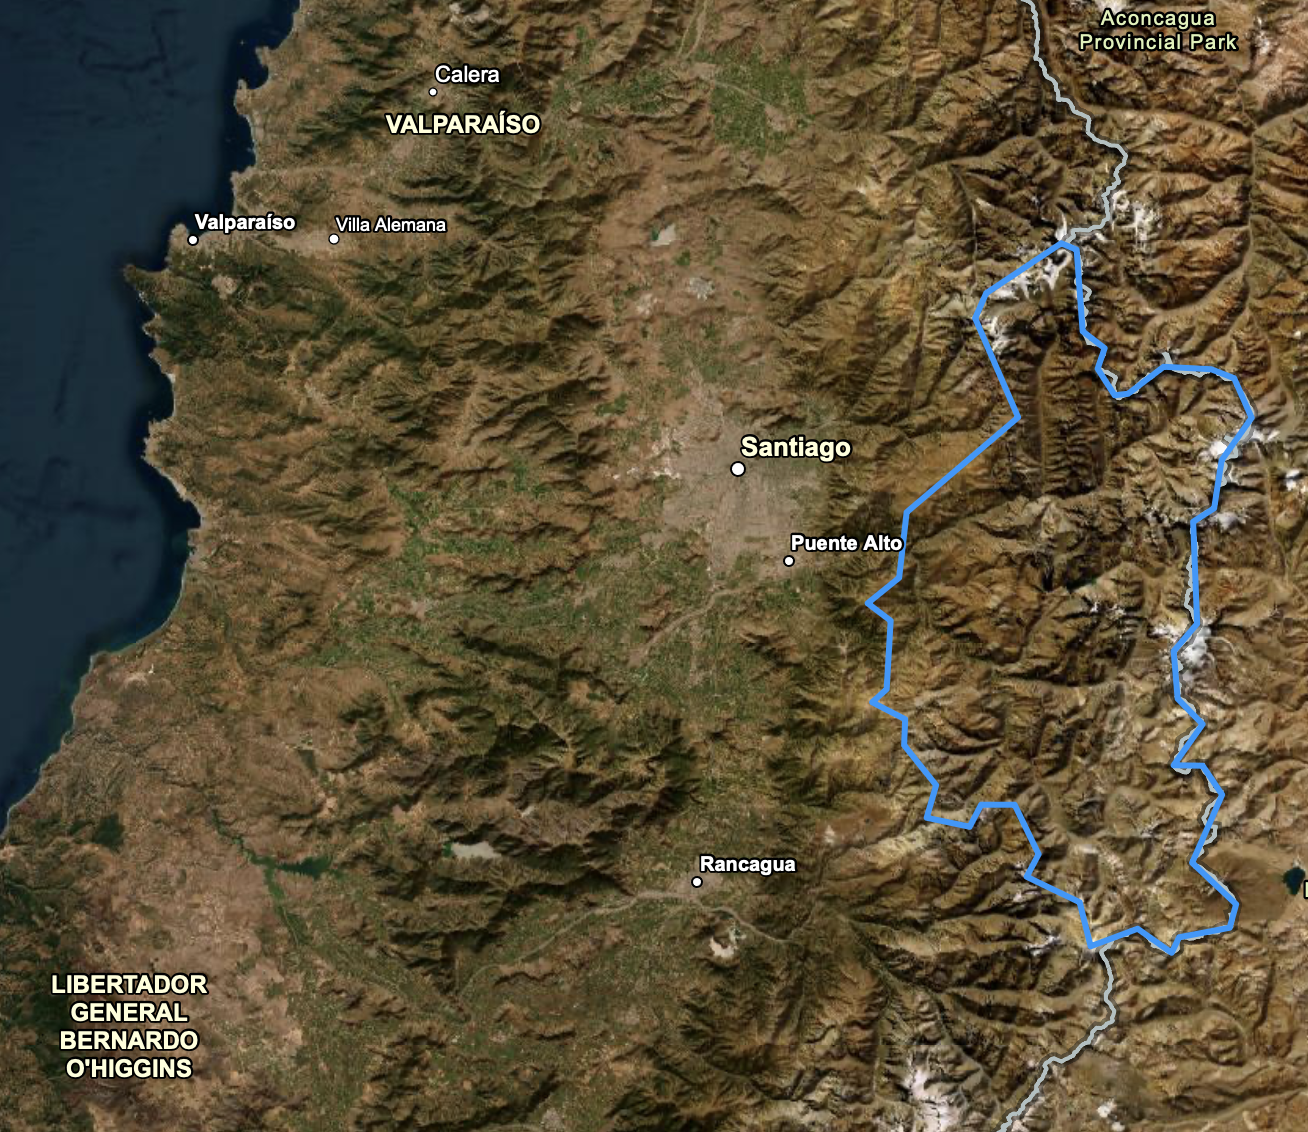
\includegraphics[width=\textwidth]{UbicaciónEspacialConDetalle.png}
\caption{Ubicación en Chile central (polígono azul), al este de Santiago.}
\end{subfigure}\hfill
\begin{subfigure}[b]{0.46\textwidth}
\centering
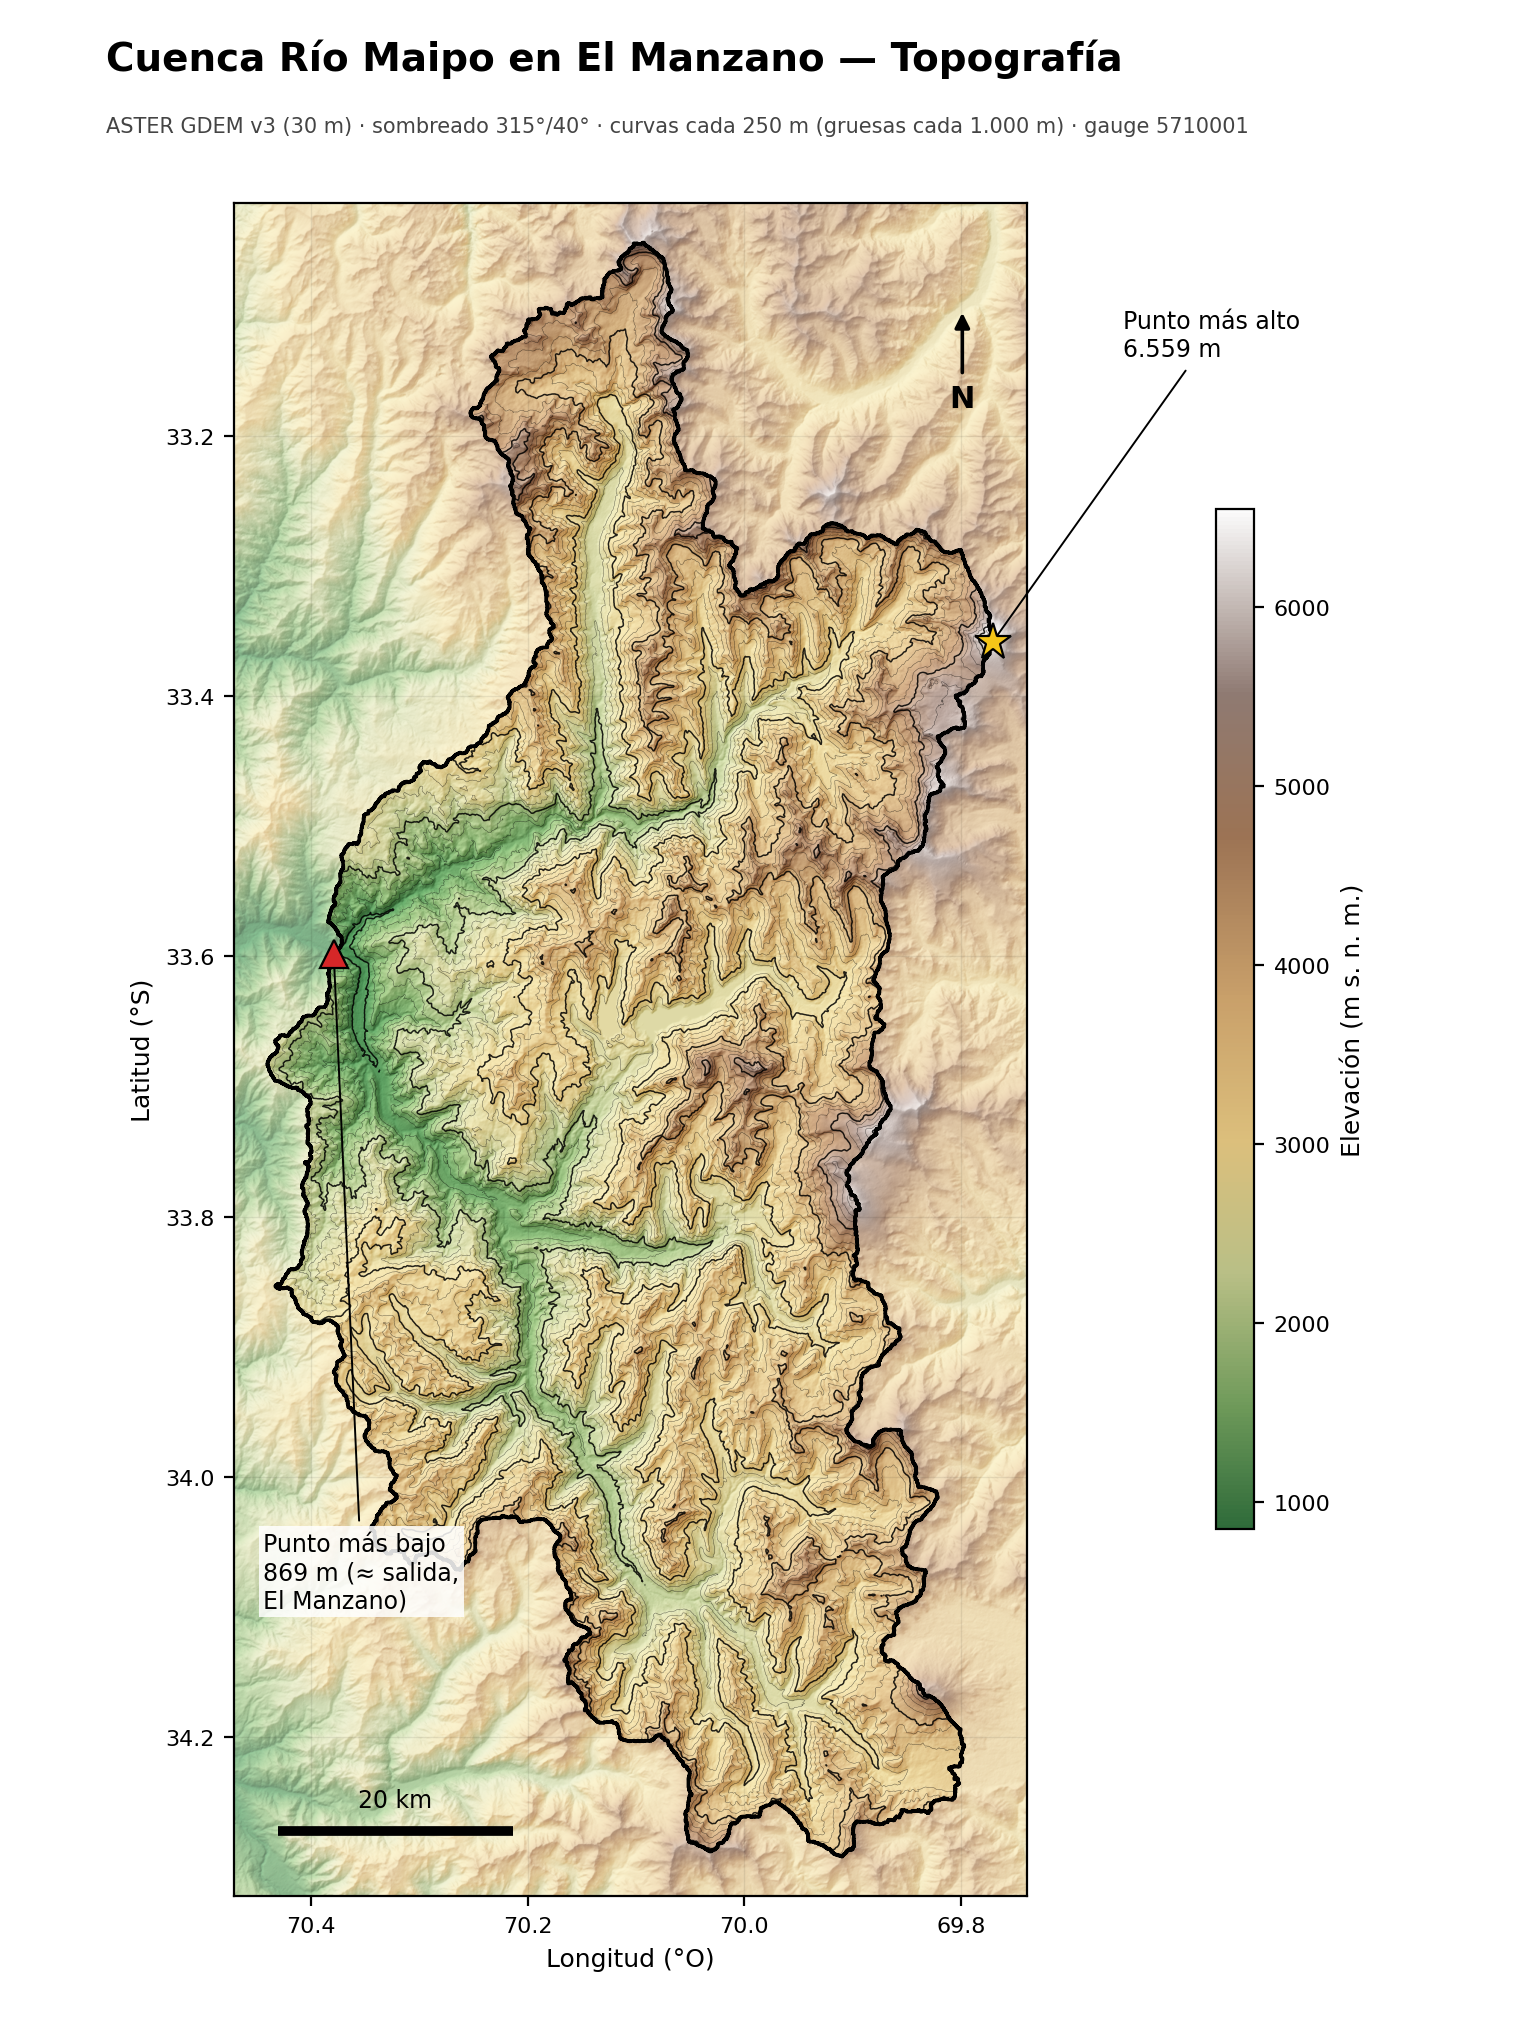
\includegraphics[width=\textwidth]{mapa_topografico_Maipo.png}
\caption{Topografía (ASTER GDEM v3, 30~m), salida y punto más alto.}
\end{subfigure}
\caption{Ubicación y relieve de la cuenca del Río Maipo en El Manzano. La delimitación es el polígono oficial de CAMELS-CL (\archivo{datos/camels_cl_5710001/polygon/polygon.shp}), trazado a partir de la topografía hasta la salida corregida de la estación DGA \citep{AlvarezGarreton2018}. El panel (a) es una captura del visor de NASA Earthdata Search (\url{https://search.earthdata.nasa.gov}) tomada durante la descarga del modelo de elevación. El panel (b) lo genera \archivo{scripts/22_p1_0_topografia_cuenca.py} a partir de ASTER GDEM v3 \citep{ASTERGDEM}.}
\label{fig:mapas}
\end{figure}

\begin{figure}[H]
\centering
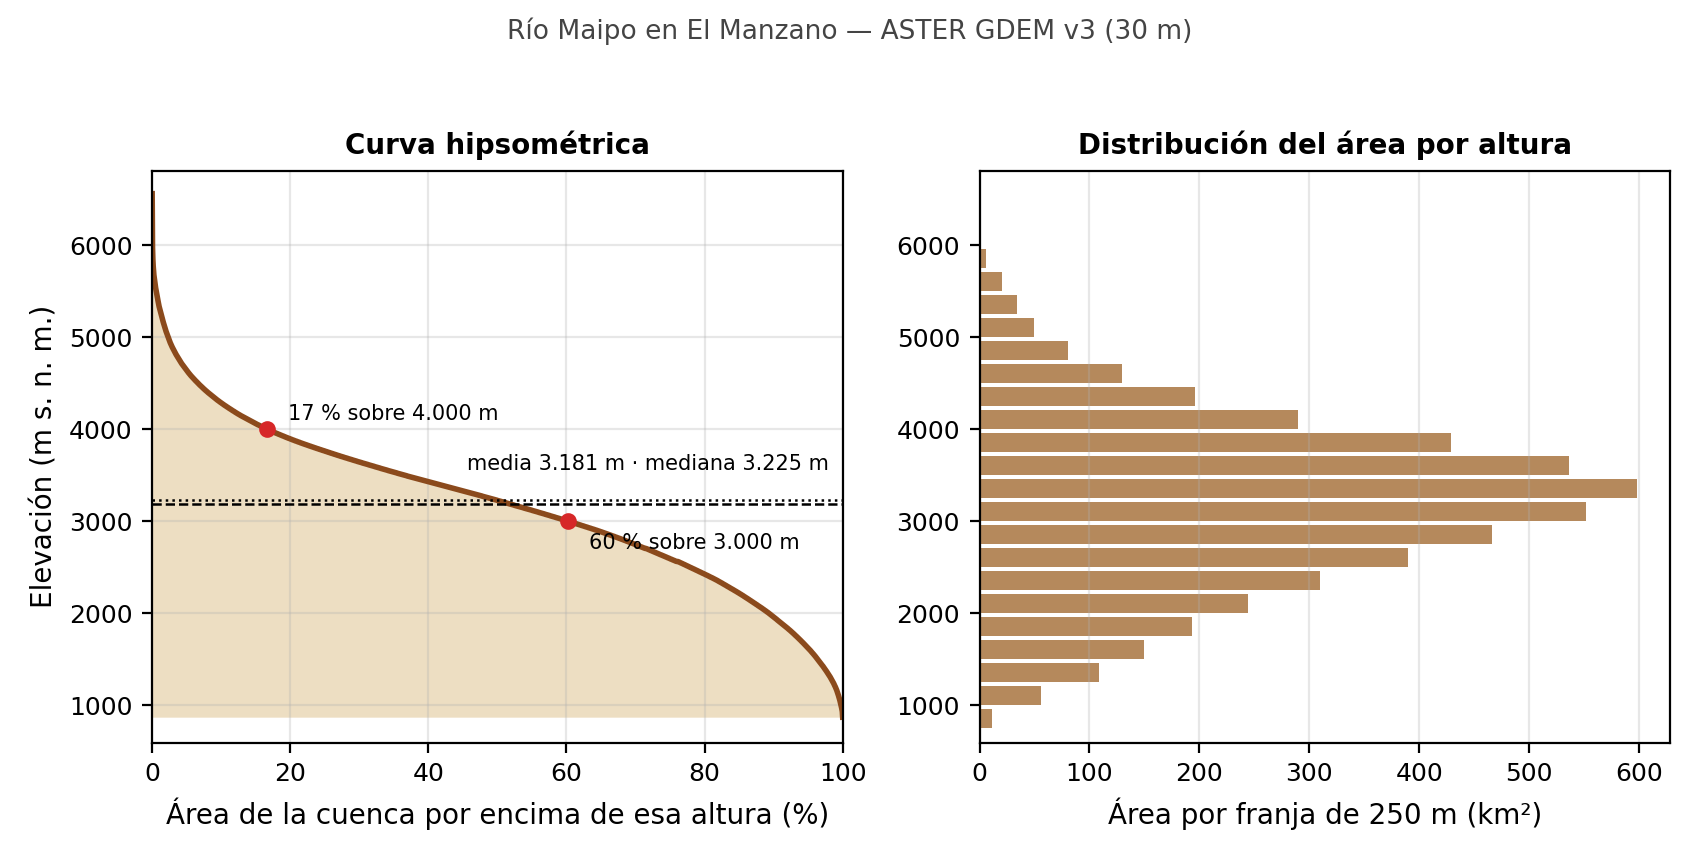
\includegraphics[width=0.86\textwidth]{curva_hipsometrica_Maipo.png}
\caption{Curva hipsométrica y distribución del área por franjas de 250~m, calculadas con el área real de cada píxel de ASTER GDEM v3 dentro del polígono CAMELS-CL \citep{ASTERGDEM} (\archivo{scripts/22_p1_0_topografia_cuenca.py}; \archivo{figuras/tabla_1_12_hipsometria.csv}). El 60\,\% del área está sobre 3000~m y el 17\,\% sobre 4000~m; la máxima superficie se encuentra entre 3250 y 3500~m.}
\label{fig:hipso}
\end{figure}

\subsection{Hipótesis inicial y objetivos}
\label{sec:hipotesis}

Con la ficha y una primera lectura de las series formulamos la \textbf{hipótesis inicial}: \emph{el Maipo en El Manzano es una cuenca de régimen nival, cuya precipitación llega casi solo en invierno con los sistemas frontales y se almacena como nieve, de modo que el caudal alcanza su máximo en primavera--verano con varios meses de retraso; por ese almacenamiento, el caudal integra la variabilidad de la lluvia de uno o más inviernos y debería responder a los modos climáticos que modulan la lluvia invernal, como ENSO}. Los objetivos fueron:

\begin{enumerate}
\item Describir la distribución, la calidad y el ciclo anual de $\PL$, $\PI$, $\Qm$ y $T$, y proponer una clasificación con criterios explícitos (punto 1).
\item Cuantificar las relaciones entre las dos precipitaciones y entre precipitación y caudal, y evaluar fuera del ajuste si existen modelos útiles (punto 2).
\item Detectar y cuantificar tendencias, su forma (gradual o salto) y su robustez, y evaluar sus posibles causas (punto 3).
\item Identificar las escalas temporales dominantes mediante análisis de Fourier (punto 4).
\item Identificar las regiones oceánicas y los patrones atmosféricos asociados con la lluvia y el caudal, mes a mes (punto 5).
\item Integrar todo en un esquema conceptual y revisar la hipótesis inicial (Secciones~\ref{sec:sintesis} y \ref{sec:conclusiones}).
\end{enumerate}

A lo largo del informe distinguimos tres niveles de afirmación: \emph{resultados observados} (cifras calculadas con su incertidumbre), \emph{productos de reanálisis o grillados} (que no son observaciones directas) e \emph{hipótesis de interpretación} (mecanismos que proponemos y contrastamos). Cada resultado sigue la secuencia que pide la guía: resultado, mecanismo, evidencia y alternativas.
% =============================================================================
\section{Metodología}
\label{sec:metodologia}
% =============================================================================

\subsection{Fuentes de datos y periodos}
\label{sec:datos}

La Tabla~\ref{tab:fuentes} resume las fuentes. Todos los análisis de los puntos 1 a 5 parten de un único archivo maestro, \archivo{datos/datos_mensuales_maipo.csv} (484 filas mensuales, 1980-01 a 2020-04). Lo construye \archivo{03_integrar_datos.py} a partir de dos archivos que también se entregan: \archivo{datos/datos_mensuales_procesados.csv}, que \archivo{01_preparar_datos.py} agrega desde los datos diarios de CAMELS-CL con el criterio de completitud de la Sección~\ref{sec:qc}, y \archivo{datos/datos_satelitales_imerg_era5.csv}, con IMERG y ERA5-Land extraídos en Google Earth Engine por \archivo{02_descargar_satelite.py}. La unión de fuentes es externa (\emph{outer join}): el registro local de 40 años no se recorta a la cobertura satelital y las celdas sin dato quedan como faltantes.

\begin{table}[H]
\centering\footnotesize
\caption{Fuentes, procesamiento y cobertura de las variables. ``Válidos'' cuenta meses con dato en el CSV maestro.}
\label{tab:fuentes}
\begin{tabularx}{\textwidth}{>{\raggedright\arraybackslash}p{1.9cm}>{\raggedright\arraybackslash}X>{\raggedright\arraybackslash}p{3.3cm}>{\raggedright\arraybackslash}p{2.6cm}}
\toprule
Variable (columna) & Producto, versión y procesamiento & Resolución y unidades & Periodo y válidos \\
\midrule
$\PL$ \texttt{P\_local\_mm} & CR2MET diario promediado en la cuenca, distribuido por CAMELS-CL \citep{AlvarezGarreton2018}. Suma mensual solo con el 100\,\% de los días válidos. CR2MET es un producto grillado que combina estaciones y reanálisis: no es una observación local independiente & Promedio areal; mm/día $\rightarrow$ mm/mes & 1980-01 a 2020-04; 484 de 484 \\
$\Qm$ \texttt{Caudal\_m3s} & Caudal medio diario observado en la estación DGA 5710001 (CAMELS-CL). Media mensual con $\geq80$\,\% de días válidos & Puntual en la salida; m$^3$/s & 1980-01 a 2020-04; 463 de 484 \\
$R$ \texttt{Q\_lamina\_mm} & Lámina equivalente $R_m=86.4\,n_m\,Q_m/A$ & mm/mes & Igual que $\Qm$ \\
$\PI$ \texttt{P\_IMERG\_mm} & GPM IMERG Final mensual, colección \texttt{NASA/GPM\_L3/IMERG\_MONTHLY\_V06} de Google Earth Engine \citep{IMERGV06,Huffman2020}; media de la cuenca con \texttt{reduceRegion} y conversión de mm/h a mm/mes multiplicando por las horas del mes & 0.1$^\circ$ ($\approx$103~km$^2$ por celda, $\approx$47 celdas en la cuenca) & 2000-06 a 2020-03; 238 \\
$T$ \texttt{Temp\_C} & Temperatura de la base, como pide la guía: media de $T_{\max}$ y $T_{\min}$ diarias CR2MET de CAMELS-CL, $\geq80$\,\% de días por mes (\archivo{01_preparar_datos.py}) & Promedio areal; $^\circ$C & 1980-01 a 2020-04; 484 \\
$T_{\mathrm{E5L}}$ \texttt{Temp\_ERA5L\_C} (contraste) & ERA5-Land mensual (\texttt{ECMWF/ERA5\_LAND/MONTHLY\_AGGR}), temperatura del aire a 2~m \citep{MunozSabater2021}; media de la cuenca y $T[^\circ\mathrm{C}]=T[\mathrm{K}]-273.15$ & 0.1$^\circ$; $^\circ$C & 2000-06 a 2020-03; 238 \\
SST, PNM, Z500 (punto 5) & ERA5 mensual de niveles únicos y de presión \citep{Hersbach2020,ERA5single,ERA5pressure}, descargado del Copernicus Climate Data Store con \archivo{scripts/15_p5_1_descargar_campos_era5.py} & 1$^\circ$ global (nativa 0.25$^\circ$); $^\circ$C, hPa, m & 1979-01 a 2020-12; sin faltantes \\
SST de contraste (punto 5) & NOAA ERSST v5 \citep{Huang2017}, reconstrucción in situ, descargada de NOAA PSL por \archivo{scripts/24_p5_3_contraste_ersst.py} & 2$^\circ$ global; $^\circ$C & 1979-01 a 2020-12 \\
\bottomrule
\end{tabularx}
\end{table}

\paragraph{Versión de IMERG.} El script 02 selecciona la colección V06. Una etiqueta ``V07'' en registros antiguos del equipo fue un error documental, corregido en la bitácora. No se conservó el archivo intermedio ni el identificador de la exportación de Earth Engine, por lo que denominamos la serie ``V06 según la configuración del script''. IMERG Final incorpora información mensual de pluviómetros y CR2MET usa estaciones: las dos precipitaciones pueden compartir información y no son fuentes completamente independientes \citep{Huffman2020,AlvarezGarreton2018}.

\paragraph{Periodos.} Usamos dos ventanas, como pide el punto 3.1: (i) el \emph{registro completo} de cada variable para preguntas de largo plazo (40 años para $\PL$, $\Qm$ y $T$; 20 años para $\PI$ y $T_{\mathrm{E5L}}$) y (ii) el \emph{periodo común} 2000-06 a 2020-03 (238 meses), el único en el que coexisten todas las fuentes, para compararlas. Las dos temperaturas nunca se unen en una sola serie. Cada análisis reporta su periodo y su número de pares válidos.

\subsection{Agregación mensual, control de calidad y faltantes}
\label{sec:qc}

\paragraph{Agregación.} Con $P_d$ en mm/día y $Q_d$ en m$^3$/s, para el mes $m$ con $n_m$ días:
\begin{equation}
P_m=\sum_{d\in m}P_d,\qquad Q_m=\frac{1}{n_m}\sum_{d\in m}Q_d,\qquad R_m=\frac{86.4}{A}\sum_{d\in m}Q_d=\frac{86.4\,n_m}{A}\,Q_m\ \text{[mm/mes]},
\label{eq:agregacion}
\end{equation}
con $A$ en km$^2$. El factor 86.4 convierte m$^3$/s acumulados durante un día sobre $A$~km$^2$ en milímetros. Usamos $A=4839.047$~km$^2$, el atributo \texttt{area\_km2} de CAMELS-CL, que el script 01 lee del archivo de atributos; es la misma área en todo el informe, el dashboard y las figuras. Comprobamos la conversión a mano para mayo de 1980: $\Qm=117.197$~m$^3$/s, $n=31$, y $86.4\times31\times117.197/4839.047=64.868$~mm, idéntico al CSV. La temperatura mensual es la media de los días del mes de $(T_{\max}+T_{\min})/2$.

\paragraph{Completitud diaria.} La guía admite como máximo un 10\,\% de días faltantes por variable en el periodo común, calculado antes de cualquier relleno. Con los archivos diarios de CAMELS-CL (\archivo{datos/camels_cl_5710001/}) y \archivo{scripts/20_p1_4_auditoria_diaria.py} obtuvimos, entre el 1 de enero de 1980 y el 30 de abril de 2020 (14\,731 días esperados):
\begin{itemize}
\item \textbf{Caudal:} 644 días faltantes (\textbf{4.37\,\%}), en 33 vacíos. Los más largos son 2015-03-23 a 2015-12-12 (265 días), 1987-11-04 a 1988-05-26 (205 días) y 1993-05-04 a 1993-06-03 (31 días). Catorce meses no tienen ningún dato y quedan como faltantes en el CSV (1987-12 a 1988-04, 1990-11 y 2015-04 a 2015-11).
\item \textbf{Precipitación y temperatura CR2MET:} 0 días faltantes.
\end{itemize}
Las tres variables cumplen el límite del 10\,\%. La Figura~\ref{fig:dispdiaria} muestra la distribución temporal de los días válidos.

\begin{figure}[H]
\centering
\begin{subfigure}[b]{0.47\textwidth}
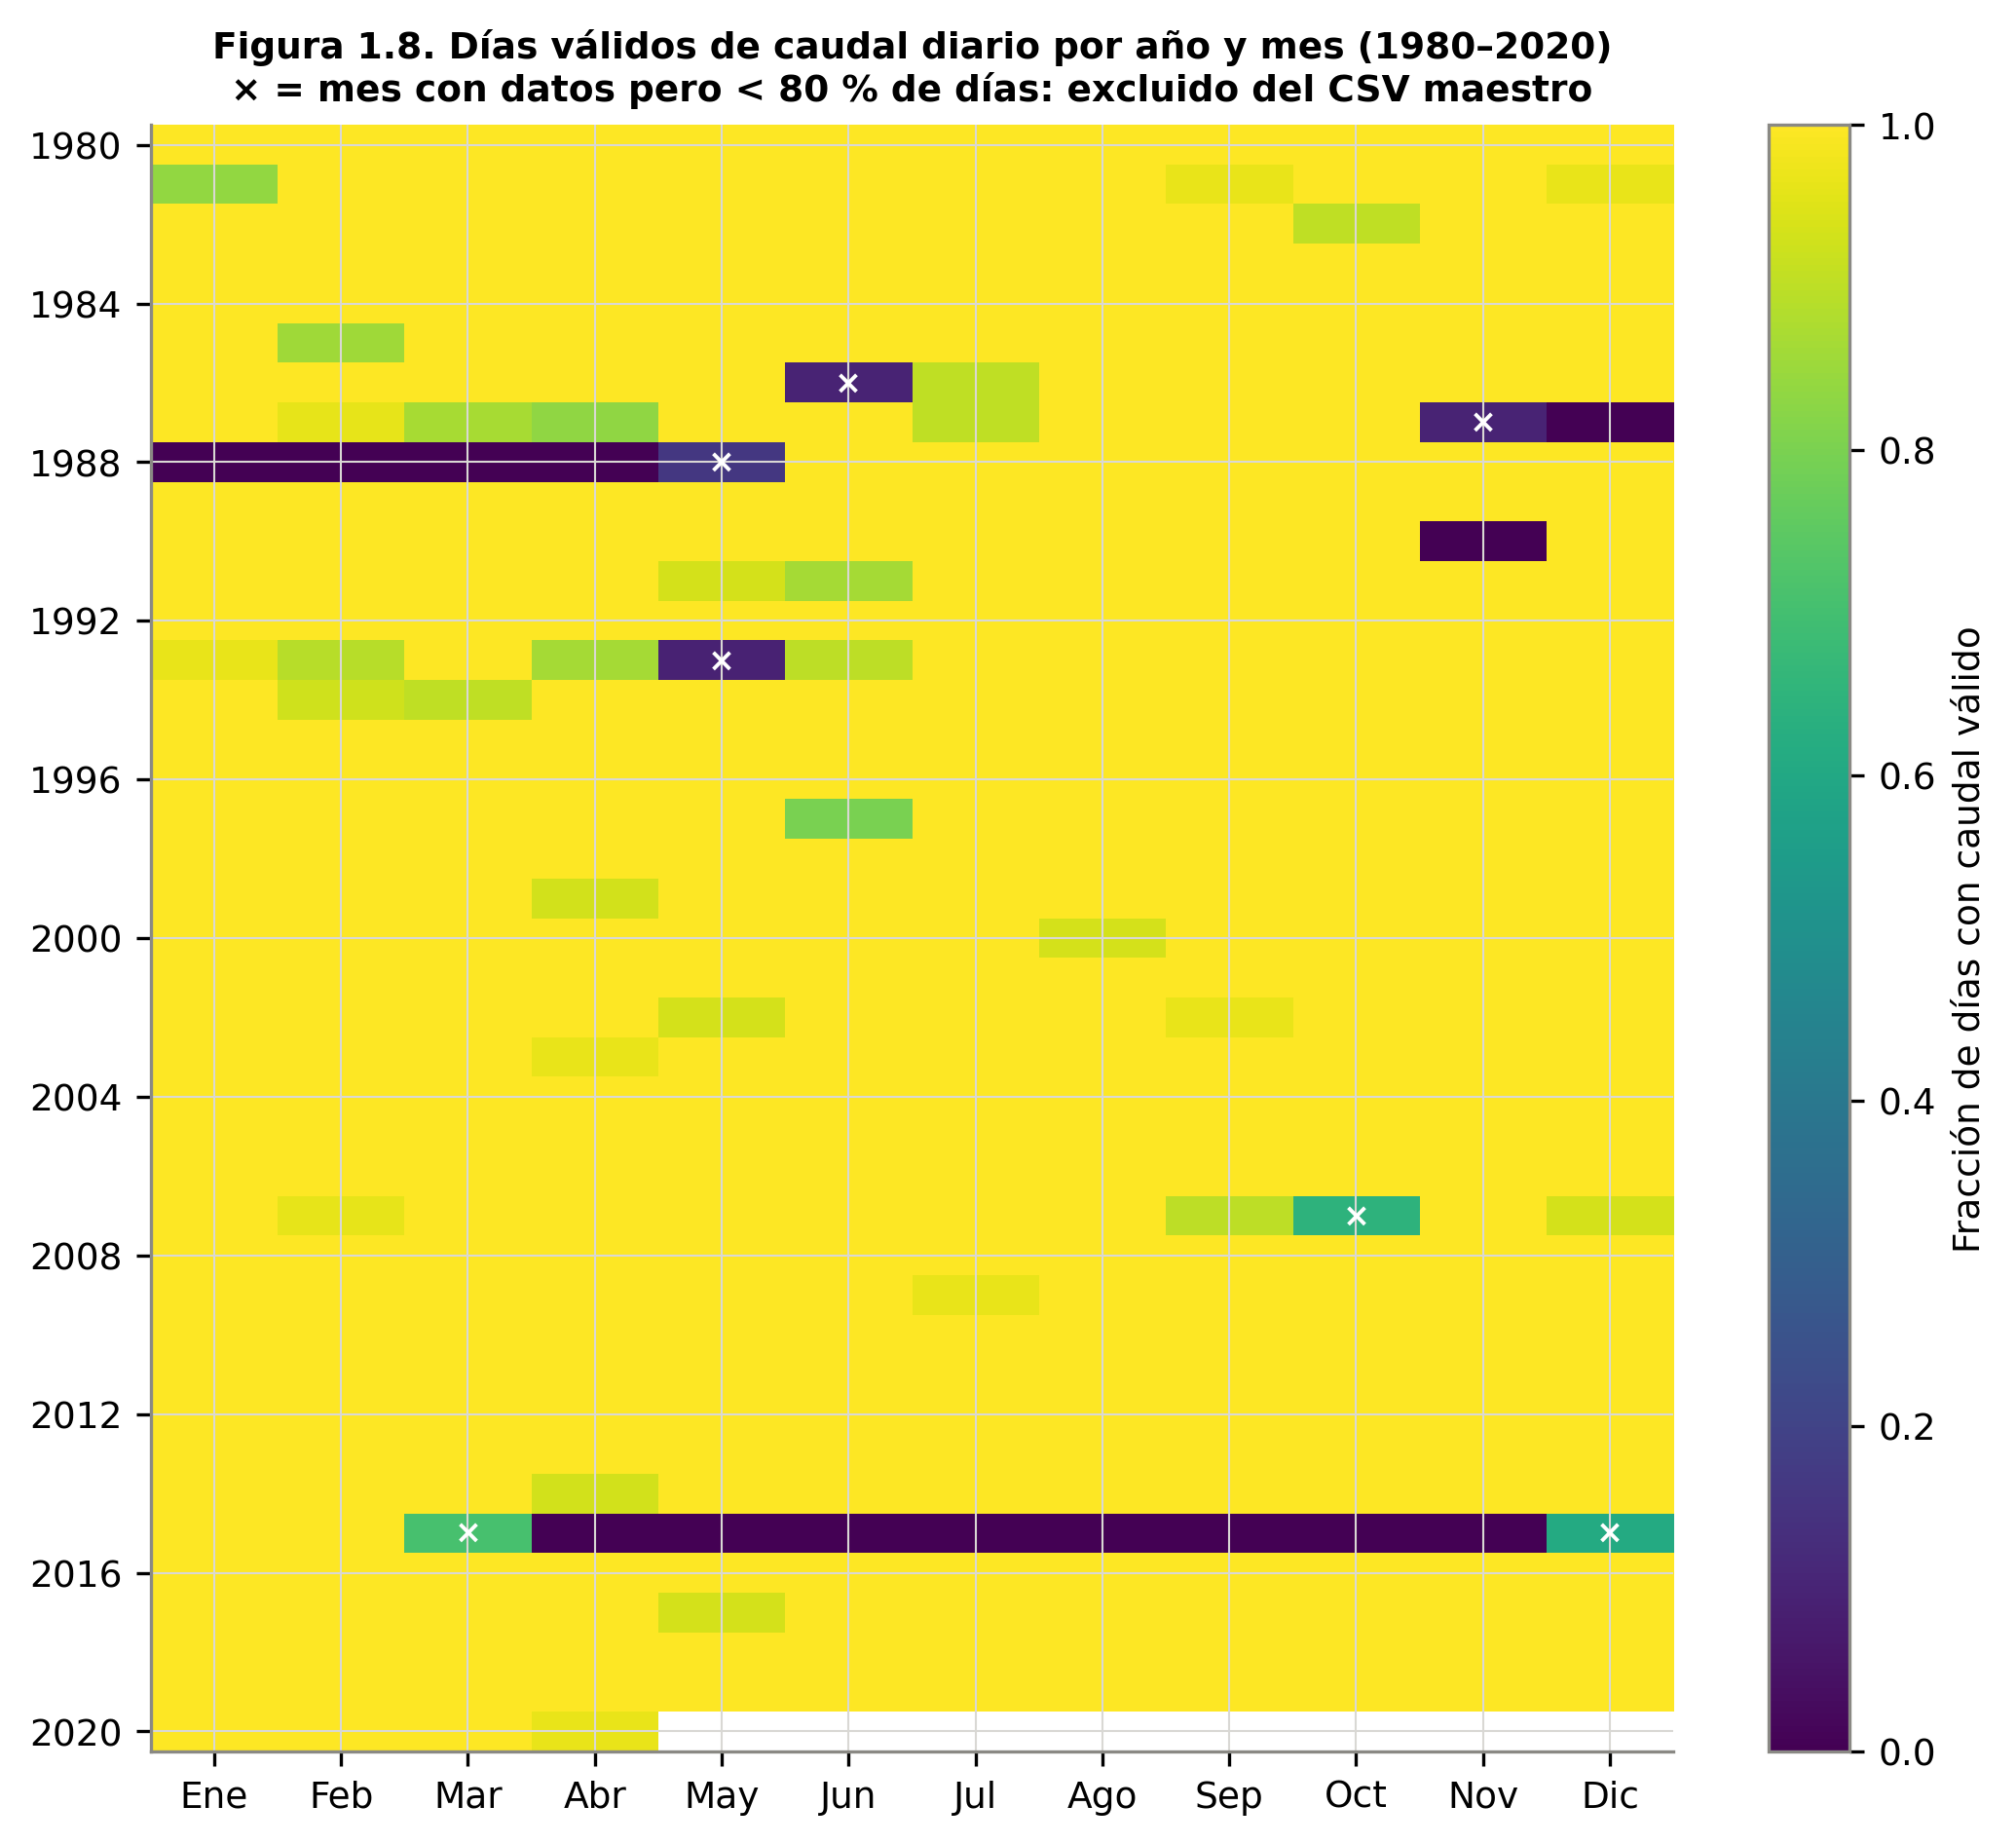
\includegraphics[width=\textwidth]{figura_1_8_disponibilidad_diaria.png}
\caption{Fracción de días válidos de caudal por año y mes; $\times$: excluido por $<80$\,\%.}
\end{subfigure}\hfill
\begin{subfigure}[b]{0.50\textwidth}
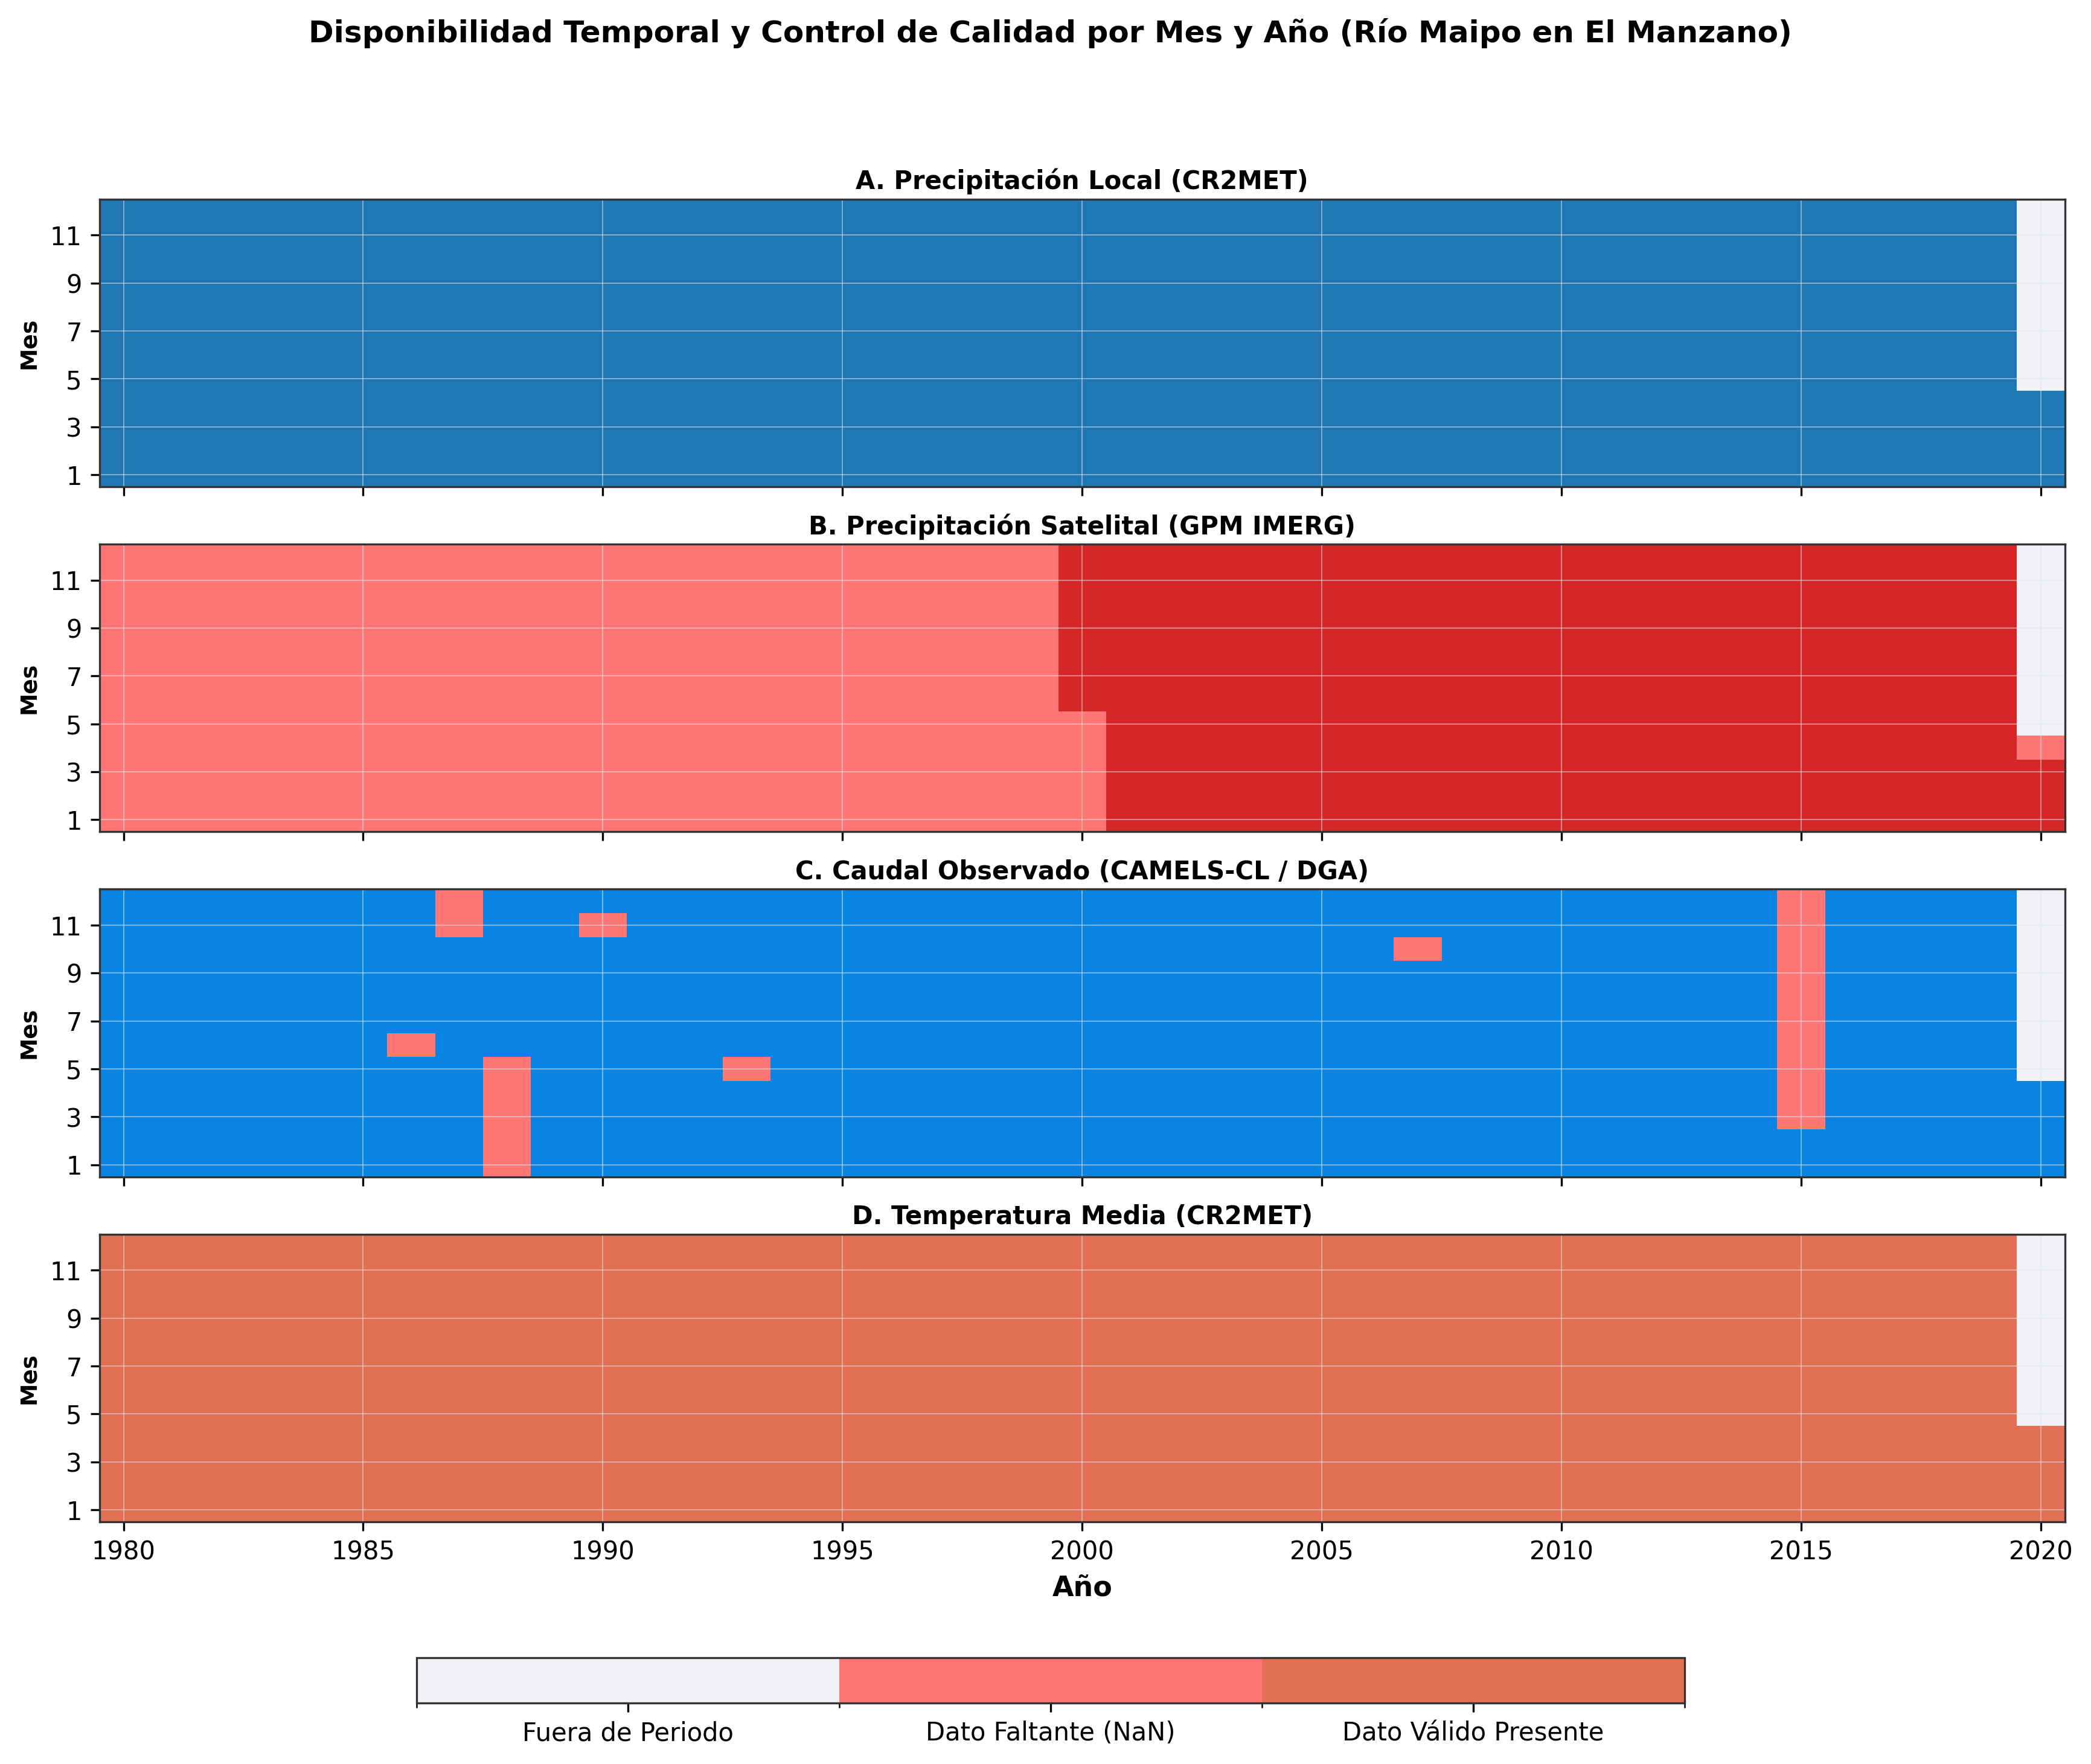
\includegraphics[width=\textwidth]{figura_1_4_disponibilidad_temporal_heatmap.png}
\caption{Meses retenidos en el CSV maestro por variable.}
\end{subfigure}
\caption{Disponibilidad de datos. (a) Días válidos de caudal diario; las cruces marcan meses con datos pero menos del 80\,\% de los días, que se excluyen (\archivo{scripts/20_p1_4_auditoria_diaria.py}). (b) Disponibilidad mensual de las cuatro variables en el archivo maestro (\archivo{scripts/07_rol_a_explorador.py}).}
\label{fig:dispdiaria}
\end{figure}

\paragraph{Criterio de completitud, aplicado en todo el análisis.} Un acumulado mensual de precipitación solo se calcula si están los 100\,\% de los días; una media mensual de caudal o de temperatura exige al menos el 80\,\% de los días del mes. Con un 80\,\% (24--25 días) la media mensual de un caudal persistente apenas cambia, mientras que con menos días un evento corto puede dominar el promedio. El criterio no excluye ningún mes de precipitación ni de temperatura. En el caudal excluye 21 meses: 14 sin ningún dato (1987-12 a 1988-04, 1990-11 y 2015-04 a 2015-11) y 7 con datos parciales, 1986-06 (3 días), 1987-11 (3), 1988-05 (5), 1993-05 (3), 2007-10 (20), 2015-03 (22) y 2015-12 (19) (\archivo{figuras/tabla_1_7_disponibilidad_diaria_mensual.csv}). El caso más importante es \textbf{mayo de 1993}: la media de los días disponibles (306.6~m$^3$/s) promedia solo el 1, 2 y 3 de mayo, y el 3 de mayo registró 722~m$^3$/s durante la crecida de una tormenta cálida, de modo que no representa la media de mayo. Una primera versión del CSV maestro calculaba el caudal sin mínimo de días y cortaba la serie diaria el 1 de abril de 2020; la Tabla~\ref{tab:sens_completitud} compara ambas versiones para los resultados principales.

\begin{table}[H]
\centering\small
\caption{Efecto del criterio de completitud sobre los resultados del caudal (\archivo{figuras/tabla_1_9_sensibilidad_completitud_Q.csv}). Tendencias sobre anomalías mensuales con la referencia 2000-06/2020-03 y las mismas funciones de \archivo{scripts/rol_c_comun.py}.}
\label{tab:sens_completitud}
\resizebox{\textwidth}{!}{\begin{tabular}{lrr}
\toprule
Resultado & Sin mínimo de días (versión anterior) & Criterio $\geq80$\,\% (CSV maestro final) \\
\midrule
Meses válidos & 470 & 463 \\
Media (m$^3$/s) & 112.4 & 111.8 \\
Máximo (m$^3$/s, fecha) & 592.8 (1983-01) & 592.8 (1983-01) \\
OLS sobre anomalías, IC 95\,\% HAC (m$^3$/s por década) & $-18.2$ [$-26.1$, $-10.3$] & $-18.0$ [$-26.0$, $-10.0$] \\
Theil--Sen (m$^3$/s por década), $p$ Mann--Kendall de Hamed--Rao & $-14.9$, $p<0.001$ & $-14.8$, $p<0.001$ \\
Cambio de Pettitt en la anomalía anual & 2007 ($p=0.014$) & 2007 ($p=0.014$) \\
\bottomrule
\end{tabular}}
\end{table}

Las conclusiones del caudal no cambian, pero el criterio elimina artefactos puntuales: el valor espurio de mayo de 1993 y su anomalía estandarizada de 16.5 desaparecen, y el máximo de caudal cae en noviembre--enero en todos los años completos (Sección~\ref{sec:clim}).

\paragraph{Otras comprobaciones.} El script \archivo{07_rol_a_explorador.py} verificó la regularidad de las fechas (0 duplicados), la ausencia de valores negativos y la consistencia de unidades (\archivo{figuras/tabla_1_3_control_calidad.csv}). Los ceros de precipitación (4 meses de $\PL$) son meses secos, no faltantes; las temperaturas negativas son físicamente posibles en una cuenca cuya altura media es de 3181~m. Ningún valor extremo se eliminó por quedar fuera de los bigotes de un diagrama de caja; los extremos se revisaron contra la serie diaria y el contexto meteorológico (Sección~\ref{sec:p1}). Los valores faltantes nunca se rellenan con ceros. La única imputación del informe es la interpolación de la anomalía de los 21 meses de caudal excluidos, solo para el análisis espectral, marcada y evaluada por separado (Sección~\ref{sec:met_p4}).

\subsection{Representatividad espacial}

La cuenca tiene unos 4840~km$^2$, frente a celdas de 0.1$^\circ$ ($\approx$11.1~km~$\times$~9.3~km~$\approx$~103~km$^2$ a 33.7$^\circ$S) en IMERG y ERA5-Land: la cuenca contiene unas 47 celdas, suficientes para un promedio areal. \texttt{reduceRegion} con \texttt{ee.Reducer.mean} pondera cada píxel por la fracción de su área dentro del polígono, lo que trata los bordes de forma proporcional; no se usó el píxel de la estación de salida. La resolución efectiva de IMERG es más gruesa que la malla y no resuelve los gradientes orográficos de pequeña escala, una fuente reconocida de error en los Andes \citep{Zambrano2017,Rojas2021}. La temperatura CR2MET es un promedio areal de un producto de 0.05$^\circ$ que corrige por altura; la de ERA5-Land representa la altura del terreno suavizado de cada celda del modelo, y su nivel difiere del de CR2MET en 5.6~$^\circ$C (Sección~\ref{sec:temp}). En el punto 5 los campos de 1$^\circ$ ($\approx$10\,000~km$^2$ por celda) solo se usan para patrones de gran escala.

\subsection{Climatología de referencia y anomalías}
\label{sec:anomalias}

Para cada variable $X_t$ con mes calendario $j(t)$ definimos
\begin{equation}
a_t = X_t-\mu_{j(t)},\qquad z_t=\frac{X_t-\mu_{j(t)}}{s_{j(t)}},
\label{eq:anomalias}
\end{equation}
donde $\mu_j$ y $s_j$ (desviación estándar muestral) se calculan sobre la \textbf{referencia fija 2000-06 a 2020-03}, con 19--20 años válidos por mes. Elegimos esta referencia porque es la única ventana común a las cuatro variables, lo que permite comparar fuentes con la misma climatología, y la usamos de forma idéntica en los puntos 2 a 5. No usamos una media única para todos los meses ni climatologías móviles. Ningún $s_j$ es nulo. La referencia cae en un periodo seco, lo que hace que los años ochenta aparezcan como anomalías positivas grandes; esa elección no altera las pendientes, porque restar una constante por mes no cambia la tendencia. Estandarizar no garantiza normalidad ni equivale a calcular un índice SPI.

\subsection{Métodos de cada punto}

\subsubsection{Punto 1: distribución y climatología}
Para cada variable calculamos meses válidos, media, mediana, desviación estándar, extremos, cuartiles, rango intercuartílico y percentiles 5, 10, 90 y 95 (interpolación lineal, convención de \texttt{numpy}), tanto en el registro completo como en el periodo común. Los histogramas de $\PL$ y $\PI$ usan los mismos 238 meses y las mismas clases (25 intervalos de 26.4~mm/mes) en frecuencia relativa. La climatología de doce meses se calcula en el periodo común con los mismos pares de meses válidos para las dos precipitaciones. Medimos la estacionalidad con el índice de Walsh y Lawler \citep{WalshLawler1981},
\begin{equation}
SI=\frac{1}{\bar R}\sum_{j=1}^{12}\left|\bar x_j-\frac{\bar R}{12}\right|,
\end{equation}
donde $\bar x_j$ es la media del mes $j$ y $\bar R$ el total anual medio. Comparamos dos subperiodos (1980--1999 y 2000--2020) y, por año hidrológico (abril--marzo), registramos el mes de máximo de $\PL$ y de $\Qm$ (\archivo{figuras/tabla_1_11_picos_y_totales_por_anio.csv}). Scripts: \archivo{07_rol_a_explorador.py} y \archivo{20_p1_4_auditoria_diaria.py}.

\subsubsection{Punto 2: relaciones y modelos}
Con pares completos para cada relación calculamos Pearson y Spearman. Para la concordancia de $\PI$ con $\PL$ definimos el error $e_t=P_{I,t}-P_{L,t}$, y con él el sesgo medio, el MAE, el RMSE y $\mathrm{PBIAS}=100\sum e_t/\sum P_{L,t}$ \citep{Willmott1981,HossainHuffman2008,Gupta2009}. Exploramos rezagos $k=0,\ldots,12$ meses entre $P(t-k)$ y $\Qm(t)$, sin usar lluvia futura, en series originales y en anomalías. Los modelos candidatos fueron:
\begin{align}
\text{lluvia:}\quad &\hat P_{L,t}=\max(0,\beta_0+\beta_1P_{I,t}) \ \ \text{o una forma log-lineal con corrección \emph{smearing}};\\
\text{caudal:}\quad &\hat Q_t=\bar Q_{j(t),\mathrm{aj}}+\alpha+\beta\,\big[P_{t-k}-\bar P_{j(t-k),\mathrm{aj}}\big],
\label{eq:modeloq}
\end{align}
comparados con referencias sencillas: IMERG sin corregir para la lluvia y la climatología mensual del caudal para el caudal. La evaluación usa tres bloques cronológicos externos no solapados (2010--2012, 2013--2015 y 2016--2020-03). En cada bloque, el modelo, el rezago $k$, los parámetros y las climatologías se seleccionan y estiman solo con los datos anteriores al bloque, con una ventana interna de tres años para elegir el rezago \citep{Klemes1986,Roberts2017,Bergmeir2018}. Scripts: \archivo{04_analisis_precipitacion.py}, \archivo{05_anomalias_rezagos.py} y \archivo{06_modelos_validacion_temporal.py}.

\subsubsection{Punto 3: tendencias}
\label{sec:met_p3}
Evaluamos dos escalas: la secuencia de todos los meses y doce subseries por mes calendario, en las tres representaciones $X$, $a$ y $z$, con el año decimal de las fechas reales como variable temporal. Usamos tres familias de métodos:
\begin{enumerate}
\item \textbf{OLS} $X_t=\beta_0+\beta_1t+\varepsilon_t$ (y sus equivalentes para $a$ y $z$), más un ajuste con efectos fijos de mes para $X$. Como los residuos están autocorrelacionados y son heterocedásticos, la inferencia usa errores HAC de Newey--West \citep{NeweyWest1987} con $\lfloor4(n/100)^{2/9}\rfloor$ rezagos. Diagnosticamos los residuos con Durbin--Watson, Ljung--Box, Breusch--Pagan y Shapiro--Wilk.
\item \textbf{Tendencia monotónica no paramétrica}: Mann--Kendall \citep{Mann1945,Kendall1975} con pendiente de Theil--Sen \citep{Sen1968}. Para la serie original con ciclo anual usamos Kendall estacional y Sen estacional \citep{Hirsch1982}, con valor $p$ por remuestreo de bloques de tres años completos (2000 réplicas). Para $a$, $z$ y las subseries mensuales usamos la corrección de varianza por autocorrelación de Hamed y Rao \citep{HamedRao1998}, acotada para que no reduzca nunca la varianza. Este es el método MK3 del estudio recomendado por la guía, que también usa bootstrap por bloques y la prueba de Pettitt \citep{Amirthanathan2023}.
\item \textbf{Evolución no lineal}: LOESS robusto \citep{Cleveland1979}, con ventana de unos 10 años en la escala global (banda del 95\,\% por bootstrap de bloques de 24 meses) y de unos 15 años mes a mes. Lo tratamos como curva exploratoria, sin inferencia formal, y evaluamos ventanas de 6, 10 y 20 años.
\end{enumerate}
Expresamos las pendientes por década en las unidades de cada representación; en precipitación son cambios del acumulado mensual (mm/mes por década), no del total anual. Fijamos $\alpha=0.05$ y controlamos la tasa de falsos descubrimientos (FDR) de Benjamini--Hochberg \citep{BH1995} en dos familias: 48 pruebas mensuales por método (12 meses $\times$ 4 variables) y 12 pruebas globales. Para la robustez quitamos los años extremos, recorrimos todas las ventanas de inicio y fin de al menos 15 años y comparamos una tendencia lineal con un escalón en el año de cambio de Pettitt \citep{Pettitt1979} mediante el AIC. Scripts: \archivo{09_p3_2_anomalias.py} a \archivo{12_p3_5_incertidumbre_robustez.py}, con funciones comunes en \archivo{rol_c_comun.py}.

\subsubsection{Punto 4: análisis espectral}
\label{sec:met_p4}
Usamos tramos de años hidrológicos completos para que el ciclo anual quepa un número entero de veces: el registro completo de 1980-04 a 2020-03 ($N=480$; $\PL$, $\Qm$ y $T$) y el periodo común de 2001-04 a 2020-03 ($N=228$; las cuatro variables). La densidad espectral unilateral,
\begin{equation}
P(f_k)=\frac{2\,\Delta t}{\sum_n w_n^2}\left|\sum_{n=0}^{N-1} w_n\,x_n\,e^{-i2\pi kn/N}\right|^2,\qquad f_k=\frac{k}{N\Delta t},\quad \Delta f=\frac{1}{N\Delta t},
\end{equation}
con $\Delta t=1$ mes, cumple $\sum_kP(f_k)\Delta f=\mathrm{var}(x)$ (Parseval, verificado). La frecuencia de Nyquist es 0.5 ciclos/mes. Comparamos tres estimadores: periodograma sin ventana (boxcar), periodograma con ventana Hann (estimador principal) y Welch con segmentos Hann de 120 meses solapados al 50\,\% \citep{Welch1967,Harris1978}. No se rellenó con ceros. Analizamos tres transformaciones: la serie centrada (C, conserva el ciclo anual), las anomalías (A) y las anomalías sin la tendencia lineal del punto 3 (AD). Los 21 meses de caudal excluidos (Sección~\ref{sec:qc}) se rellenaron interpolando la anomalía; el efecto se evaluó con el tramo continuo más largo sin vacíos, que el script detecta automáticamente (1993-06 a 2007-09, $N=172$), y con un periodograma de Lomb--Scargle sobre los datos sin rellenar \citep{Lomb1976,Scargle1982}. La hipótesis nula de las anomalías es un ruido rojo AR(1) con el $r_1$ y la varianza de cada serie \citep{Gilman1963,Torrence1998}. Con 1000 simulaciones procesadas con el mismo estimador obtuvimos umbrales del 95\,\% puntuales y globales; el umbral global corrige la búsqueda entre todas las frecuencias. Scripts: \archivo{13_p4_1_preparacion_espectral.py} y \archivo{14_p4_2_espectros_interpretacion.py}.

\subsubsection{Punto 5: mapas de correlación}
Elegimos la SST y dos campos atmosféricos por su papel en la cadena que lleva la lluvia invernal a la cuenca: la presión al nivel del mar (PNM), que describe el anticiclón subtropical que bloquea o deja pasar los frentes, y la altura geopotencial de 500~hPa (Z500), que identifica vaguadas y bajas segregadas en la tropósfera media. ERA5 entrega geopotencial $\Phi$ (m$^2$\,s$^{-2}$); usamos la altura geopotencial $Z=\Phi/g_0$ con $g_0=9.80665$~m\,s$^{-2}$. En 500~hPa no hay celdas bajo la superficie sobre la región. La SST se enmascara sobre tierra y bajo hielo marino ($\leq-1.6$~$^\circ$C). Para cada mes calendario $j$ de la cuenca y cada celda:
\begin{equation}
r_j(\lambda,\phi;\ell)=\operatorname{corr}_{\{t:\,j(t)=j\}}\big[a_X(t),\,a_Y(\lambda,\phi,t-\ell)\big],
\end{equation}
es decir, la correlación entre todos los meses $j$ de la cuenca y el campo $\ell$ meses antes ($\ell>0$: el campo antecede; enero con $\ell=1$ se empareja con diciembre del año anterior). Las anomalías de los campos usan la misma referencia fija. Exigimos al menos 15 años por celda. La significancia se evalúa con una prueba $t$ con tamaño efectivo $n_{\mathrm{eff}}=n(1-r_{1x}r_{1y})/(1+r_{1x}r_{1y})$ \citep{Bretherton1999} y FDR con $\alpha_{\mathrm{FDR}}=0.10$ por mapa \citep{Wilks2016}. Para la robustez comparamos mapas sin tendencia en ambas series, sin los tres años extremos, de $\PL$ frente a IMERG y de dos subperiodos, mediante correlaciones de patrón en el Pacífico. Además definimos \emph{a priori} tres índices: Niño 3.4 (SST, 5$^\circ$S--5$^\circ$N, 170$^\circ$--120$^\circ$W) \citep{Trenberth1997}, PNM del Pacífico sureste (30--40$^\circ$S, 75--90$^\circ$W) y Z500 de Chile central (30--40$^\circ$S, 70--85$^\circ$W). Scripts: \archivo{15_p5_1_descargar_campos_era5.py} a \archivo{19_p5_4_interpretacion.py}, con funciones comunes en \archivo{p5_comun.py}.
% =============================================================================
\section{Resultados y discusión física}
\label{sec:resultados}
% =============================================================================

\subsection{Punto 1. Series mensuales: exploración y validación}
\label{sec:p1}

\subsubsection{Series cronológicas (1.1 y 1.2)}

La Figura~\ref{fig:series} muestra las cinco series en paneles alineados, con el mismo eje temporal y los vacíos visibles. A simple vista, la precipitación llega en pulsos invernales muy desiguales entre años: 1982, 1984, 1987, 1997, 2000, 2002 y 2005--2006 tienen meses de más de 400~mm. El caudal, en cambio, dibuja un ciclo regular con un máximo por año. Los años húmedos dejan un caudal alto en el verano siguiente: el máximo de enero de 1983 (592.8~m$^3$/s) sigue al junio de 1982 (705~mm). La década de 2010 muestra un descenso persistente de ambos, con mínimos en 2019. La temperatura CR2MET oscila entre $-5.1$ y $+13.4$~$^\circ$C; ERA5-Land sigue el mismo ciclo, pero unos 5.6~$^\circ$C más fría. IMERG sigue la forma de la precipitación de referencia en el periodo común, pero con picos más bajos.

\begin{figure}[H]
\centering
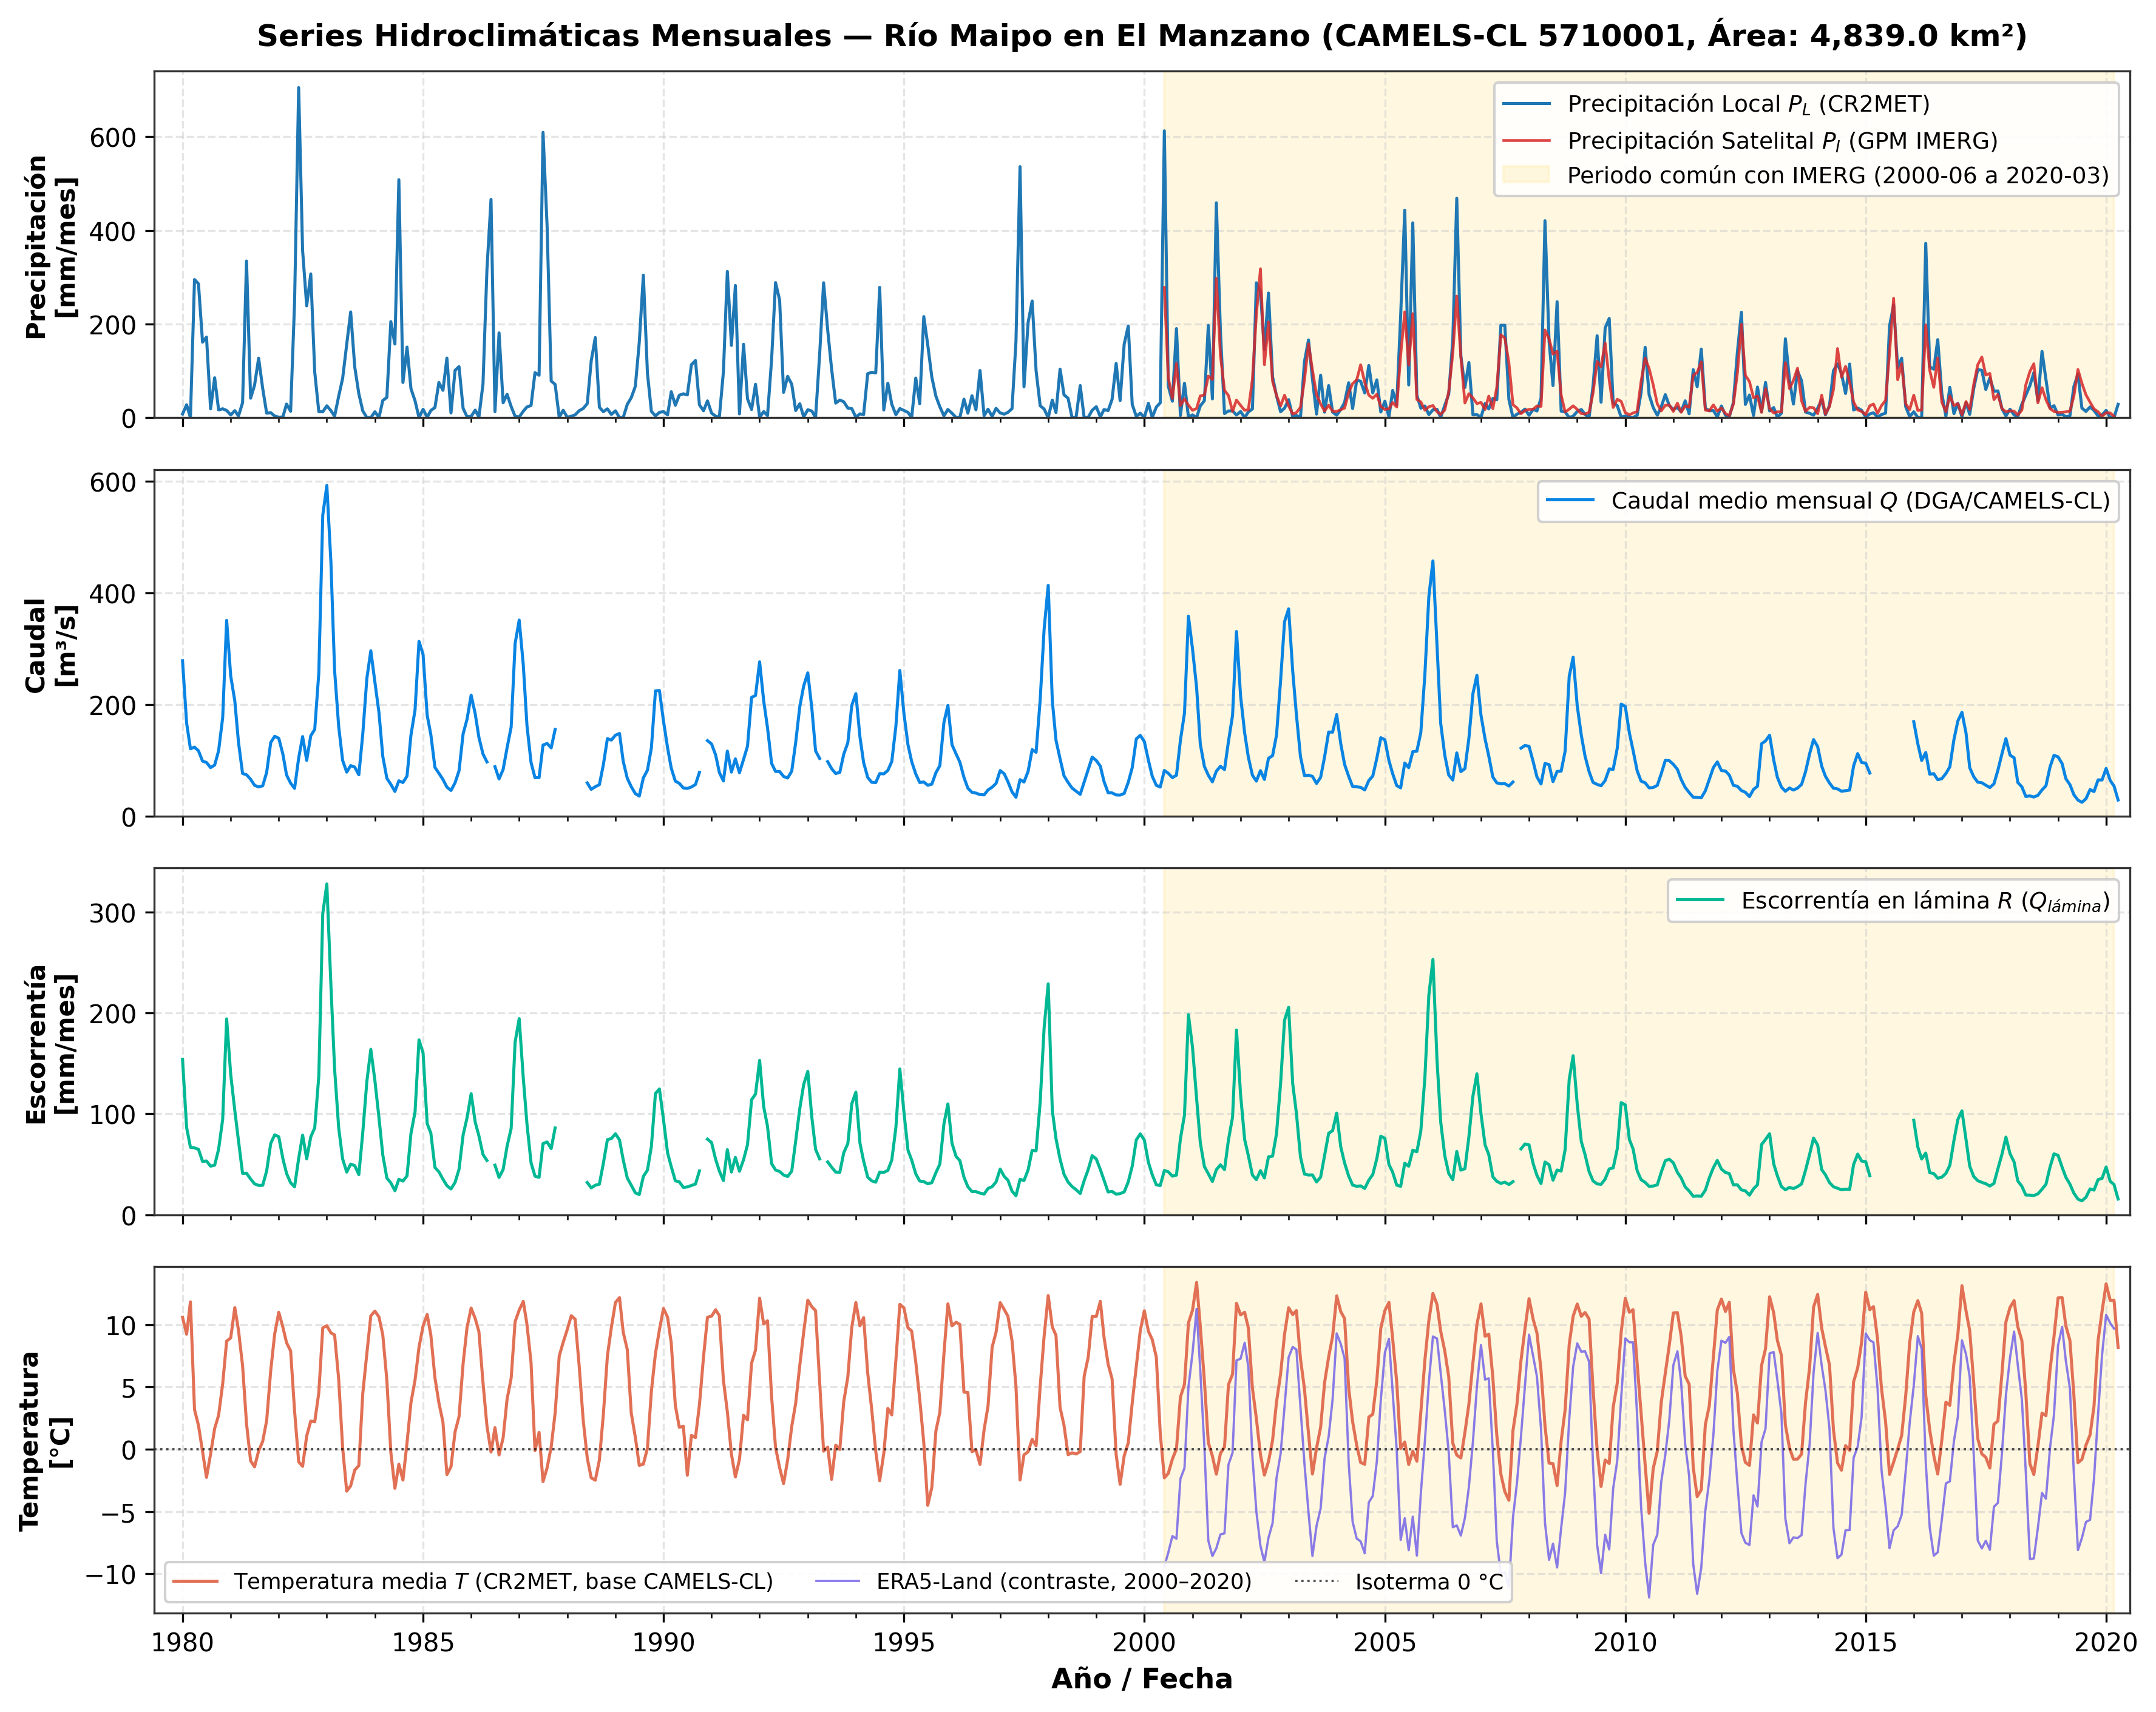
\includegraphics[width=0.95\textwidth]{figura_1_1_series_cronologicas.png}
\caption{Series mensuales de precipitación de referencia ($\PL$, CR2MET) e IMERG ($\PI$), caudal ($\Qm$), lámina de escorrentía ($R$) y temperatura CR2MET ($T$), con ERA5-Land como contraste. Sombreado: periodo común 2000-06 a 2020-03. Los cortes de línea son meses faltantes o excluidos por el criterio de completitud, que no se rellenan. Script \archivo{07_rol_a_explorador.py}.}
\label{fig:series}
\end{figure}

\subsubsection{Distribución de los datos mensuales (1.3)}

\begin{table}[H]
\centering\footnotesize\setlength{\tabcolsep}{3.2pt}
\caption{Estadísticos de las series mensuales (\archivo{figuras/tabla_1_1_distribucion_estadistica.csv}). C: registro completo de cada variable; Co: periodo común 2000-06 a 2020-03. Percentiles por interpolación lineal; los faltantes se excluyen. $\PL$, $\PI$ y $R$ en mm/mes; $\Qm$ en m$^3$/s; $T$ (CR2MET) y $T_{\mathrm{E5L}}$ (ERA5-Land) en $^\circ$C.}
\label{tab:distribucion}
\begin{tabular}{llrrrrrrrrrrrrr}
\toprule
Var. & & $n$ & Media & Mediana & DE & Mín. & P5 & P10 & Q1 & Q3 & P90 & P95 & Máx. & Asim. \\
\midrule
$\PL$ & C & 484 & 67.88 & 25.88 & 101.12 & 0.00 & 0.42 & 1.49 & 9.64 & 84.58 & 186.28 & 281.76 & 705.04 & 2.81 \\
$\PL$ & Co & 238 & 62.79 & 25.56 & 92.29 & 0.00 & 0.61 & 1.97 & 8.53 & 78.47 & 167.20 & 227.39 & 612.67 & 2.87 \\
$\PI$ & Co & 238 & 57.29 & 32.76 & 58.70 & 2.83 & 8.42 & 11.33 & 16.54 & 80.52 & 131.02 & 178.46 & 318.05 & 1.89 \\
$\Qm$ & C & 463 & 111.83 & 86.92 & 77.72 & 24.81 & 41.70 & 49.06 & 60.97 & 135.63 & 207.17 & 261.13 & 592.84 & 2.32 \\
$\Qm$ & Co & 227 & 102.62 & 81.57 & 69.61 & 24.81 & 39.67 & 47.05 & 58.44 & 119.95 & 182.01 & 251.90 & 457.58 & 2.28 \\
$R$ & C & 463 & 60.70 & 47.11 & 42.36 & 13.73 & 22.89 & 26.69 & 33.42 & 73.78 & 110.95 & 144.29 & 328.14 & 2.38 \\
$T$ & C & 484 & 4.93 & 4.98 & 4.84 & $-5.14$ & $-2.08$ & $-1.22$ & 0.24 & 9.55 & 11.18 & 11.79 & 13.39 & $-0.03$ \\
$T_{\mathrm{E5L}}$ & Co & 238 & $-0.52$ & $-1.04$ & 6.36 & $-11.89$ & $-8.90$ & $-8.15$ & $-6.49$ & 5.67 & 8.51 & 9.02 & 11.27 & 0.17 \\
\bottomrule
\end{tabular}
\end{table}

\begin{figure}[H]
\centering
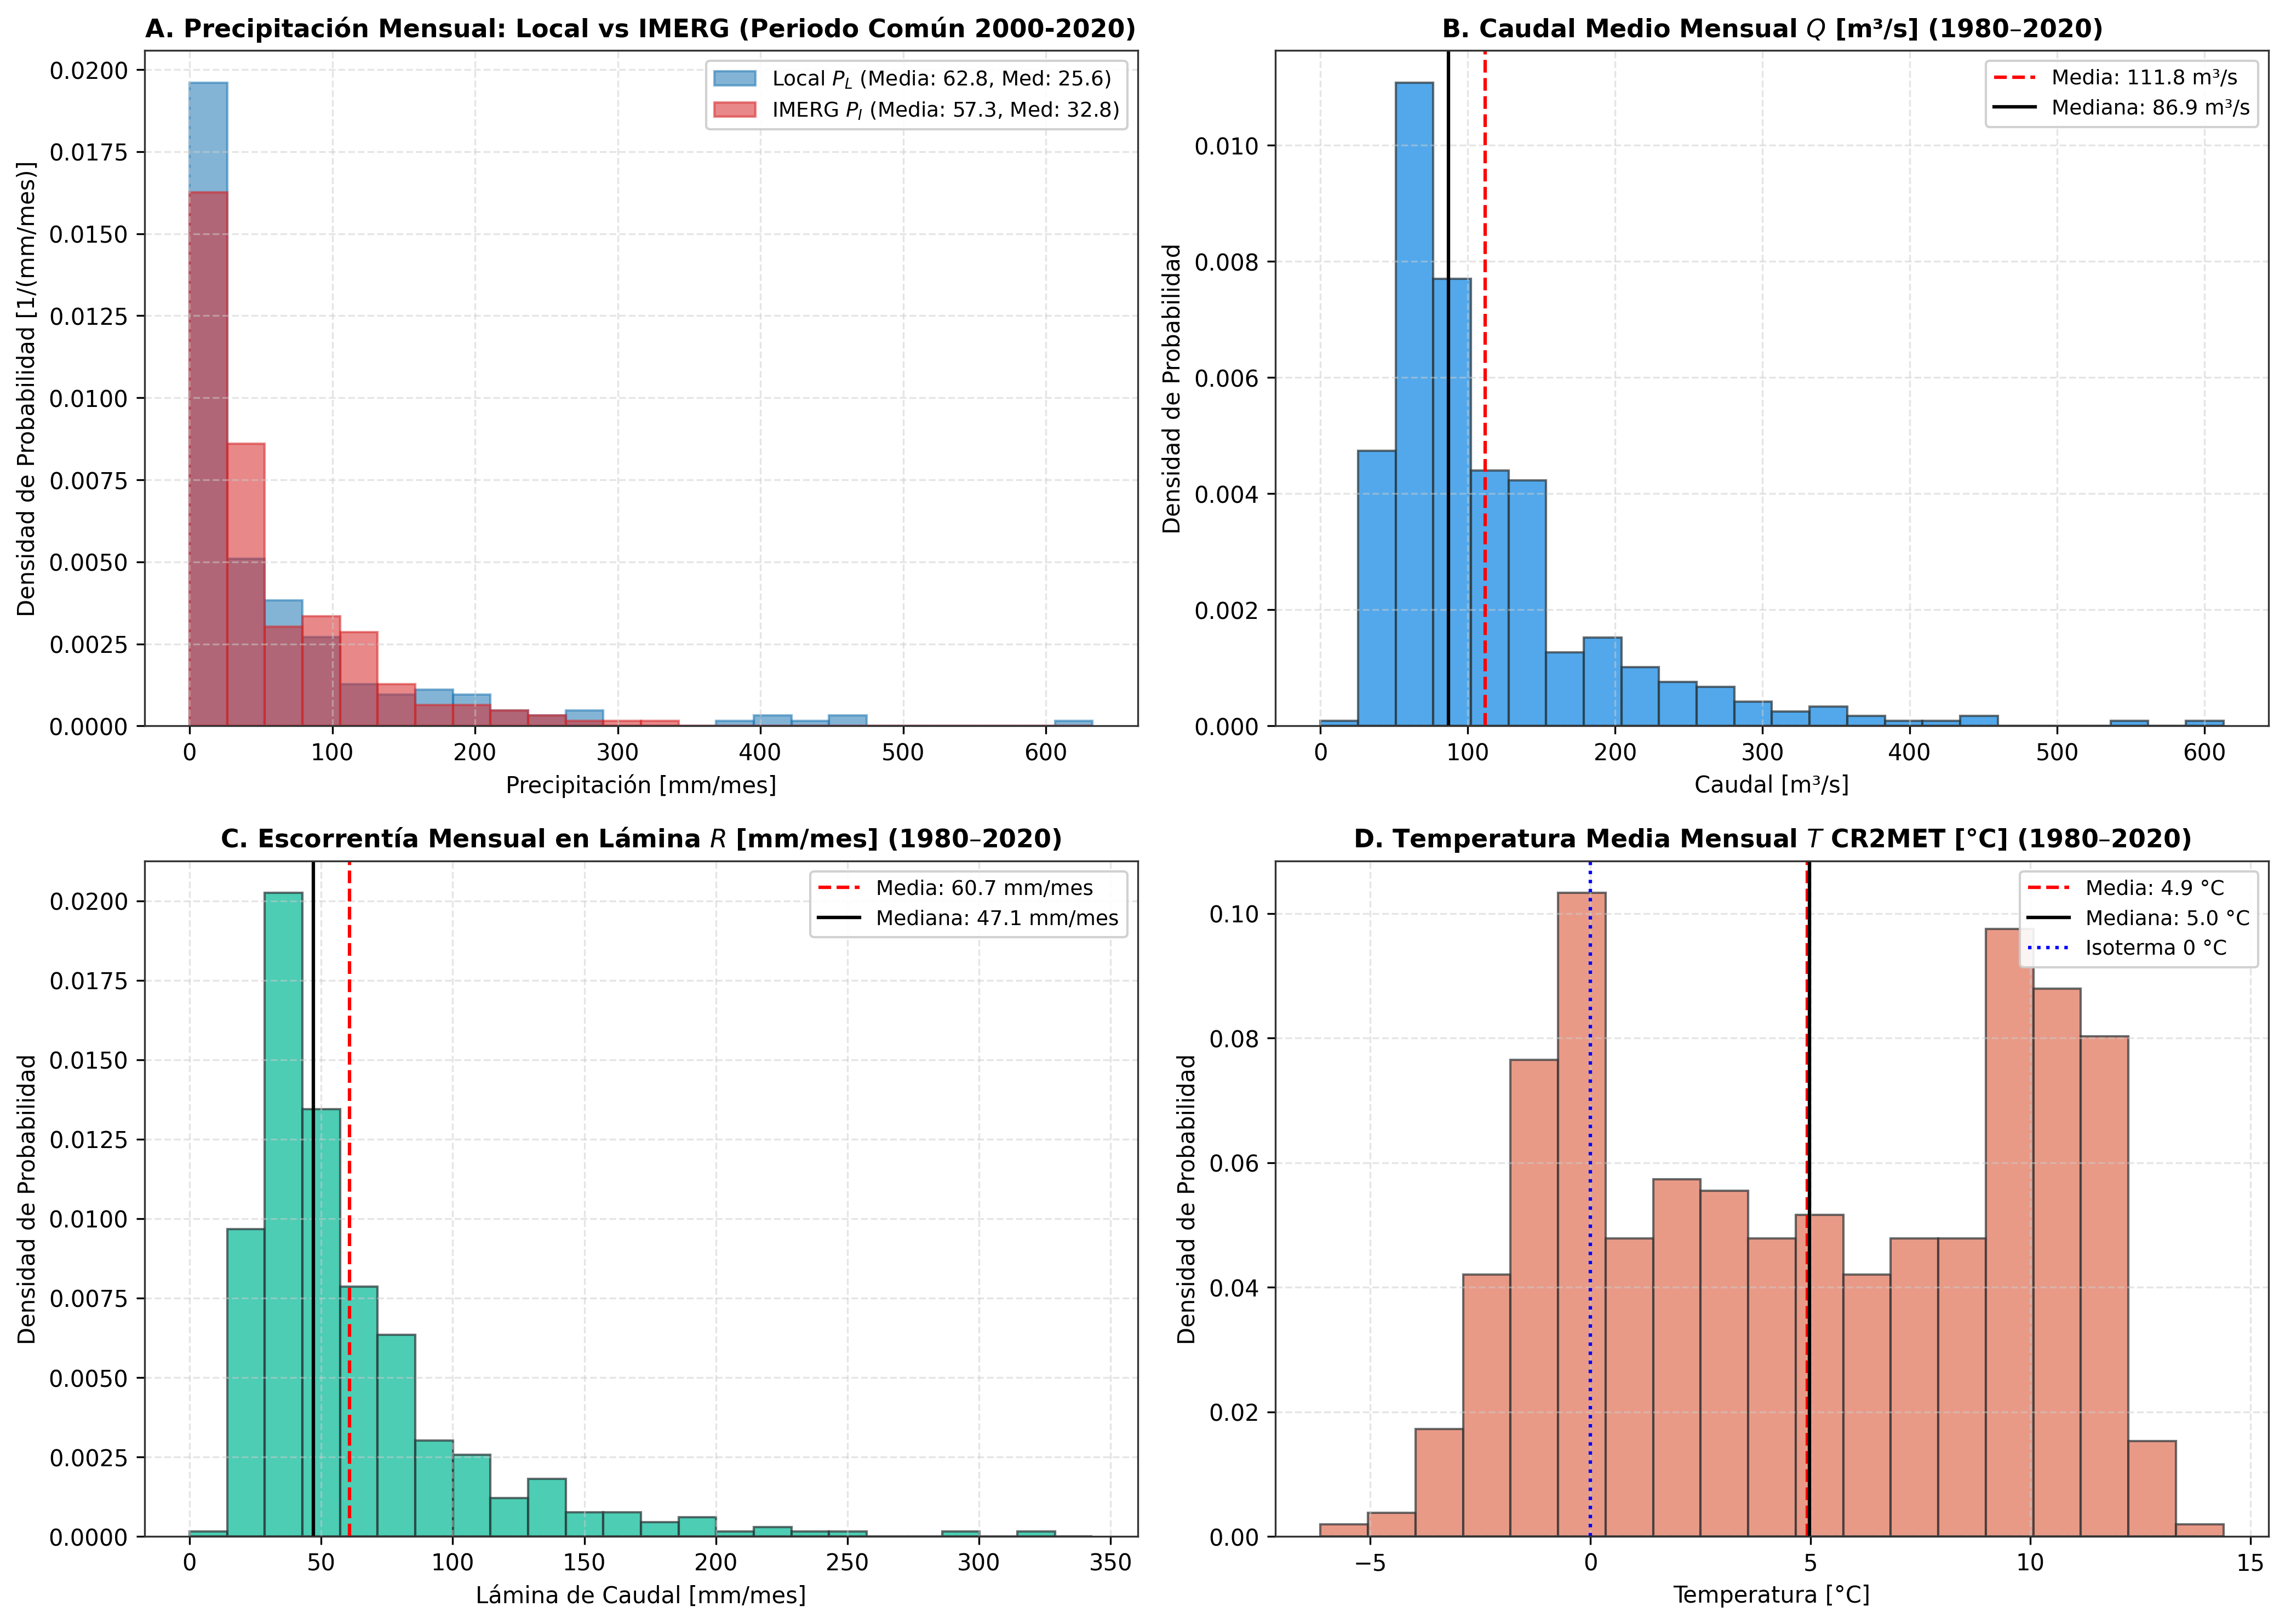
\includegraphics[width=0.95\textwidth]{figura_1_2_histogramas_distribucion.png}
\caption{Histogramas de las variables mensuales. $\PL$ y $\PI$ se comparan con los mismos 238 meses comunes y las mismas clases, en frecuencia relativa. Script \archivo{07_rol_a_explorador.py}.}
\label{fig:hist}
\end{figure}

La precipitación es muy asimétrica (Tabla~\ref{tab:distribucion}, Figuras~\ref{fig:hist} y \ref{fig:cajas}): la media de $\PL$ (68~mm/mes) casi triplica la mediana (26~mm/mes), la asimetría es $+2.8$ y el 5\,\% de los meses supera los 282~mm. Los histogramas mezclan meses de todas las estaciones, de modo que esa forma refleja sobre todo el contraste entre un verano casi seco y unos pocos meses invernales muy lluviosos, no la variabilidad entre años de un mismo mes (Sección~\ref{sec:clim}). La mediana representa mejor el mes típico; la media está dominada por los extremos invernales. Solo cuatro meses tienen $\PL=0$ (0.8\,\%) y ninguno es un dato ausente.

Las dos precipitaciones difieren en las colas. En los mismos 238 meses, IMERG tiene menor dispersión (DE de 58.7 frente a 92.3~mm/mes), menor asimetría (1.89 frente a 2.87), ningún mes seco (mínimo de 2.8~mm) y un máximo de 318~mm frente a 613~mm de $\PL$. IMERG atenúa los dos extremos: sobreestima los meses secos y subestima los muy lluviosos, comportamiento documentado en terrenos complejos de Chile \citep{Zambrano2017,SotoAlvarez2020,Rojas2021}. El caudal también es asimétrico (asimetría de 2.3), pero su mínimo nunca baja de 24.8~m$^3$/s: el río nunca se seca, lo que ya sugiere un aporte de almacenamiento. La temperatura es casi simétrica (asimetría de $-0.03$), con una media de 4.9~$^\circ$C en CR2MET y de $-0.5$~$^\circ$C en ERA5-Land: el nivel depende del producto, no la forma de la distribución (Sección~\ref{sec:temp}).

\subsubsection{Meses extremos y control de calidad (1.3 y 1.4)}

\begin{table}[H]
\centering\footnotesize
\caption{Meses extremos y su revisión (\archivo{figuras/tabla_1_2_meses_extremos.csv}, \archivo{figuras/tabla_1_7_disponibilidad_diaria_mensual.csv}).}
\label{tab:extremos}
\begin{tabularx}{\textwidth}{llr>{\raggedright\arraybackslash}X}
\toprule
Variable & Fecha & Valor & Revisión y decisión \\
\midrule
$\PL$ máx. & 1982-06 & 705.0~mm & Invierno de El Niño 1982--83, el más lluvioso del registro; coherente con el caudal récord del verano siguiente. Se conserva \\
$\PL$ máx. & 2000-06 & 612.7~mm & IMERG registra 278~mm el mismo mes: es el mayor error del periodo común (punto 2). Episodio plausible; se conserva \\
$\PL$ máx. & 1987-07 & 609.4~mm & Invierno de El Niño 1987; se conserva \\
$\Qm$ máx. & 1983-01 & 592.8~m$^3$/s & Deshielo de la nieve récord de 1982, seis meses después; mes completo (31 días). Se conserva \\
$\Qm$ & 1993-05 & -- & \textbf{Solo 3 días válidos} (1 a 3 de mayo; 722~m$^3$/s el día 3, crecida por tormenta cálida). Episodio real, pero su media (306.6~m$^3$/s) no representa el mes: generaba una anomalía estandarizada de 16.5 y el único año con el máximo de caudal fuera de noviembre--enero. \textbf{Excluido} por el criterio de completitud \\
$\Qm$ mín. & 2019-07 & 24.8~m$^3$/s & Invierno del año más seco del registro (megasequía); mes completo. Se conserva \\
$T$ mín. / máx. & 2010-07 / 2001-02 & $-5.1$ / $13.4$~$^\circ$C & Mismas fechas extremas en ERA5-Land ($-11.9$ / $11.3$~$^\circ$C); plausibles para la altura de la cuenca. Se conservan \\
\bottomrule
\end{tabularx}
\end{table}

Los extremos son coherentes entre variables: los inviernos lluviosos de El Niño (1982, 1987, 1997) aparecen como caudales altos en el verano siguiente, y el año seco de 2019 como el estiaje mínimo. La auditoría diaria aportó la principal corrección del control de calidad: el mayo de 1993, que ahora se excluye. Como advierte la guía, comparar fuentes permite detectar inconsistencias, pero no demuestra cuál es la correcta. Tampoco el residuo $P-R$ equivale a evapotranspiración: varios años secos tienen $R>P$ (Sección~\ref{sec:clim}), lo que refleja liberación de agua almacenada y no un error.

\subsubsection{Climatología, variabilidad y explicación física (1.5)}
\label{sec:clim}

\begin{figure}[H]
\centering
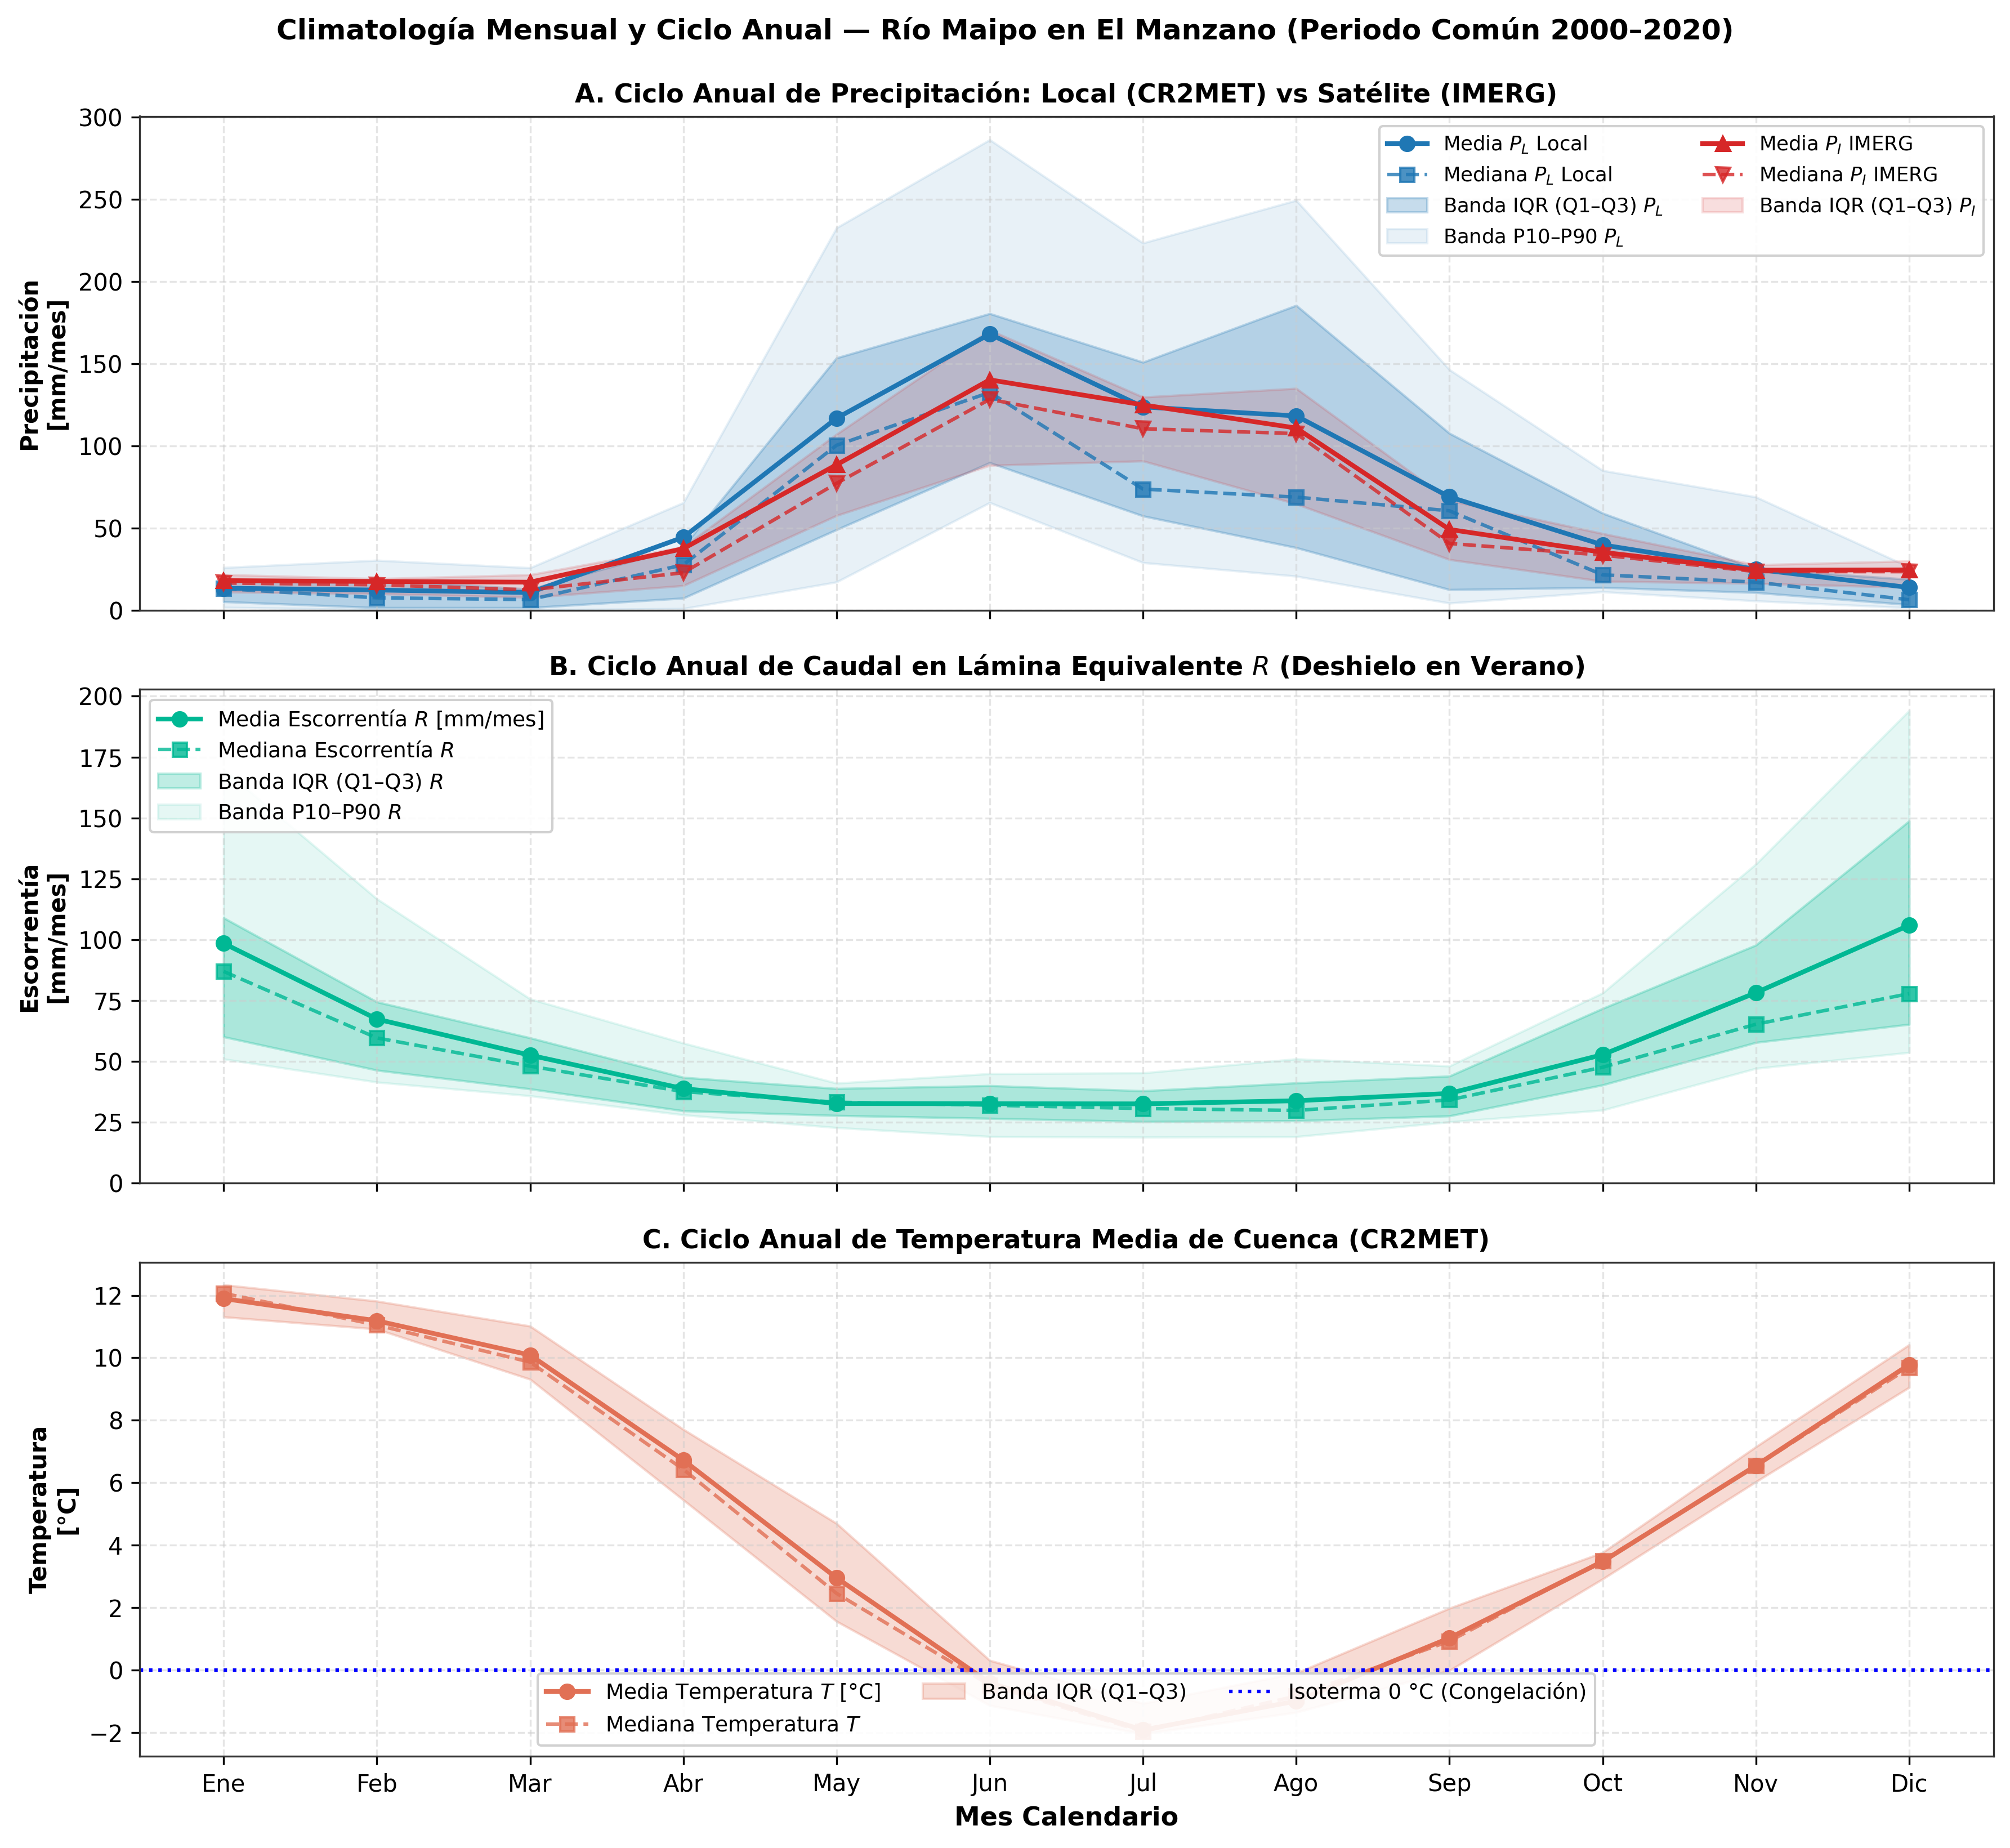
\includegraphics[width=0.92\textwidth]{figura_1_5_ciclo_anual_climatologia.png}
\caption{Ciclo anual en el periodo común 2000-06 a 2020-03: media y mediana con bandas intercuartílicas y P10--P90 de $\PL$ e IMERG (A), de la lámina $R$ (B) y de la temperatura CR2MET (C). Las bandas describen la dispersión entre años, no intervalos de confianza de la media. Script \archivo{07_rol_a_explorador.py}; datos en \archivo{figuras/tabla_1_4_climatologia_mensual.csv}.}
\label{fig:ciclo}
\end{figure}

\begin{table}[H]
\centering\footnotesize\setlength{\tabcolsep}{3.5pt}
\caption{Climatología mensual (media; entre paréntesis, la mediana) en el periodo común 2000-06 a 2020-03, con 18--20 años válidos por mes. Fuente: \archivo{figuras/tabla_1_4_climatologia_mensual.csv}.}
\label{tab:clim}
\resizebox{\textwidth}{!}{\begin{tabular}{lrrrrrrrrrrrr}
\toprule
 & Ene & Feb & Mar & Abr & May & Jun & Jul & Ago & Sep & Oct & Nov & Dic \\
\midrule
$\PL$ [mm] & 13 (13) & 12 (8) & 11 (6) & 44 (28) & 117 (100) & \textbf{168} (133) & 124 (74) & 118 (69) & 69 (61) & 40 (22) & 25 (17) & 14 (6) \\
$\PI$ [mm] & 18 (17) & 17 (15) & 17 (12) & 37 (23) & 89 (77) & \textbf{140} (128) & 125 (110) & 111 (108) & 49 (41) & 35 (34) & 24 (24) & 25 (23) \\
$\Qm$ [m$^3$/s] & 178 (157) & 134 (117) & 95 (87) & 73 (70) & 59 (60) & 61 (60) & \textbf{59} (56) & 61 (54) & 69 (64) & 95 (86) & 146 (122) & \textbf{191} (141) \\
$R$ [mm] & 99 & 67 & 53 & 39 & 33 & 33 & 33 & 34 & 37 & 53 & 78 & 106 \\
$T$ CR2MET [$^\circ$C] & 11.9 & 11.2 & 10.1 & 6.7 & 3.0 & $-0.4$ & $-1.9$ & $-1.0$ & 1.0 & 3.5 & 6.6 & 9.8 \\
$T_{\mathrm{E5L}}$ [$^\circ$C] & 8.3 & 8.5 & 6.9 & 1.8 & $-4.3$ & $-7.8$ & $-8.4$ & $-7.3$ & $-5.7$ & $-2.9$ & 0.3 & 4.4 \\
CV de $\PL$ & 0.79 & 0.98 & 1.33 & 1.85 & 0.90 & 0.84 & 1.03 & 0.92 & 0.92 & 0.91 & 0.95 & 1.24 \\
CV de $\Qm$ & 0.55 & 0.48 & 0.37 & 0.28 & 0.25 & 0.31 & 0.36 & 0.39 & 0.30 & 0.36 & 0.40 & 0.54 \\
\bottomrule
\end{tabular}}
\end{table}

\paragraph{Forma del ciclo (1.5.b).} El ciclo de la precipitación es \textbf{unimodal}, con una estación húmeda de mayo a agosto que concentra el 70\,\% del total anual medio (528 de 755~mm), máximo en junio (168~mm) y mínimo en marzo (11~mm). El índice de Walsh y Lawler es $SI_P=0.745$, en la clase ``estacional'' (0.6--0.8) \citep{WalshLawler1981}. El ciclo del caudal también es unimodal, pero está invertido: máximo en diciembre--enero (191 y 178~m$^3$/s) y mínimo de mayo a agosto (59--61~m$^3$/s), con $SI_R=0.389$, un régimen mucho más uniforme que el de la lluvia. La temperatura media de la cuenca es mínima en julio ($-1.9$~$^\circ$C en CR2MET) y sube con fuerza desde octubre, cuando el caudal empieza a crecer; la Sección~\ref{sec:isoterma} traduce ese ciclo en la parte de la cuenca que está bajo cero. El \textbf{desfase} entre los máximos medios de lluvia (junio) y de caudal (diciembre) es de seis meses. Con las medianas, que reducen el peso de los inviernos extremos, el desfase es el mismo. Los picos medios aparecen en casi todos los años: en los 32 años hidrológicos (abril--marzo) con los doce meses de caudal válidos, el máximo de $\PL$ cae entre mayo y agosto en el 78\,\% de los años (el resto en abril o septiembre) y el máximo de $\Qm$ cae entre noviembre y enero en los 32 años (en diciembre o enero en 31). La única excepción de la versión anterior del CSV, 1993, se debía al mayo incompleto (Tabla~\ref{tab:extremos}).

\paragraph{Variabilidad entre años.} Los coeficientes de variación de $\PL$ son de 0.8 a 1.9, mayores en los meses de transición (abril, diciembre y marzo), donde la media está cerca de cero y el coeficiente se vuelve inestable. Los del caudal son de 0.25 a 0.55, la mitad o menos: la cuenca amortigua la variabilidad de la lluvia. El mes más variable del caudal es diciembre--enero, porque el deshielo depende de la nieve acumulada, que varía mucho de un invierno a otro. Las curvas anuales individuales (Figura~\ref{fig:curvas}) muestran que la forma se repite cada año y que lo que cambia es la amplitud.

\paragraph{Años contrastantes y balance anual.} El año hidrológico más húmedo es 1982--83 ($\PL=2034$~mm, $R=1549$~mm, $R/P=0.76$) y el más seco 2019--20 ($\PL=259$~mm, $R=329$~mm, $R/P=1.27$). En los años húmedos $R/P<1$ (1997: 0.69; 2005: 0.93) y en los secos $R/P>1$ (1996: 1.24; 1998: 1.46; 2019: 1.27), con mediana de 0.89 en 32 años y $R/P>1$ en 8 de ellos (\archivo{figuras/tabla_1_11_picos_y_totales_por_anio.csv}). Que la cuenca entregue más agua de la que recibe en los años secos es una señal física clara: parte del caudal proviene de agua almacenada en años anteriores (nieve remanente, glaciares y agua subterránea), lo que anticipa la memoria hidrológica de los puntos 2 a 4. El coeficiente medio $R/P\approx0.88$ en el periodo común (755 y 663~mm/año) es muy alto para una cuenca de clima mediterráneo semiárido. Admite dos lecturas no excluyentes: pérdidas por evapotranspiración y sublimación pequeñas, porque la precipitación llega cuando hace frío y la cuenca es casi desnuda, o una subestimación de la precipitación de alta montaña por CR2MET, junto con aportes glaciares \citep{Ayala2020,AlvarezGarreton2018}.

\paragraph{Subperiodos (1.5.b).} Entre 1980--1999 y 2000--2020 (Figura~\ref{fig:subper}) la escorrentía disminuye en los doce meses (de $-8$\,\% en junio a $-25$\,\% en enero) y la precipitación cae en los meses de lluvia (abril $-35$\,\%, mayo $-26$\,\%, julio $-27$\,\%, septiembre $-31$\,\%). Sin embargo, la \emph{forma} del régimen se mantiene: los máximos y mínimos no cambian de mes. La clasificación es estable; la diferencia de magnitud se analiza como tendencia en el punto 3, sin atribuirla aquí a una causa.

\paragraph{Procesos (1.5.c).} La estacionalidad de la lluvia la controla la circulación regional. En verano, el anticiclón subtropical del Pacífico Sur está en su posición más austral y bloquea los sistemas frontales. En invierno se debilita y se desplaza hacia el norte, el cinturón de los oestes alcanza los 33--34$^\circ$S y los frentes, a veces asociados con ríos atmosféricos, descargan precipitación reforzada por el ascenso orográfico sobre los Andes \citep{FalveyGarreaud2007,Viale2011,Garreaud2009}. La cuenca transforma ese aporte con tres almacenamientos. (i) La nieve: entre junio y agosto más de la mitad de la cuenca está bajo 0~$^\circ$C y entre el 46 y el 78\,\% de la precipitación cae sobre esa parte (Sección~\ref{sec:isoterma}); el agua se acumula y se libera cuando la isoterma de 0~$^\circ$C sube por encima de la mayor parte de la cuenca en octubre--noviembre \citep{Masiokas2006}. (ii) Los glaciares (7.2\,\% del área), que sostienen el caudal a fines del verano y en años secos \citep{Ayala2020}. (iii) El agua subterránea en rocas volcánicas y depósitos, coherente con un índice de flujo base de 0.81 y un estiaje que nunca baja de 25~m$^3$/s. La evapotranspiración es pequeña porque la energía disponible es máxima en verano, cuando casi no llueve y la cuenca es en su mayoría roca desnuda.

\paragraph{Temperatura de la base frente a ERA5-Land.}
\label{sec:temp}
Como pide la guía, la temperatura del análisis es la de la base (CR2MET, 1980--2020), y ERA5-Land se usa como contraste sin unir las dos series. En los 238 meses comunes los dos productos tienen el mismo ciclo (correlación de 0.99, y de 0.96 en las anomalías), pero ERA5-Land es en promedio 5.6~$^\circ$C más fría ($-0.5$ frente a 5.0~$^\circ$C) y su ciclo es más amplio (16.9 frente a 13.8~$^\circ$C); la media mensual es negativa de mayo a octubre en ERA5-Land y solo de junio a agosto en CR2MET (\archivo{figuras/tabla_3_1_temperatura_cr2met_vs_era5.csv}). La diferencia proviene de cómo cada producto representa la altura y la inversión térmica en terreno complejo: CR2MET combina estaciones y temperatura de superficie satelital a 0.05$^\circ$, y ERA5-Land hereda la topografía suavizada de su malla. Sin estaciones de altura no podemos decidir cuál es correcta, de modo que tratamos la diferencia como incertidumbre y propagamos ambos productos a las conclusiones sobre la nieve.

\paragraph{Isoterma de 0~$^\circ$C y área bajo cero.}
\label{sec:isoterma}
Una media de cuenca bajo o sobre 0~$^\circ$C no dice qué parte de la cuenca acumula nieve, porque la cuenca abarca 5700~m de desnivel. Para conectar la temperatura con la topografía, \archivo{scripts/23_p1_5_isoterma_cero.py} asigna la temperatura media mensual a la elevación media de la hipsometría (3182~m), la extrapola con un gradiente vertical $\Gamma$ y calcula la altura de la isoterma de 0~$^\circ$C, $z_0=\bar z+1000\,T/\Gamma$, y la fracción del área por encima de ella. Usamos $\Gamma=6.5$~$^\circ$C/km (atmósfera estándar) y evaluamos 5.5 y 7.5~$^\circ$C/km. La Figura~\ref{fig:isoterma} muestra el resultado:
\begin{itemize}
\item Con CR2MET, la isoterma baja de unos 4900~m en enero a 2900~m en julio: de junio a agosto queda por debajo de la elevación mediana (3225~m), con el 54--64\,\% del área bajo cero, y en septiembre todavía cubre el 45\,\%. En noviembre sube a 4200~m y deja bajo cero solo el 12\,\% de la cuenca, el mes en que el caudal crece con fuerza. El gradiente apenas cambia estas cifras en invierno; solo en verano mueve la isoterma unos 300~m (\archivo{figuras/tabla_1_13_isoterma_cero_climatologia.csv}).
\item Ponderando por la lluvia mensual, entre el 46\,\% (CR2MET) y el 78\,\% (ERA5-Land) de la precipitación cae sobre área bajo 0~$^\circ$C. El rango contiene la fracción de lluvia de días con temperatura media de la cuenca bajo cero (60\,\% con CR2MET diario) y el atributo de CAMELS-CL (71\,\%). Como el realce orográfico concentra más lluvia en altura, el valor con lluvia uniforme es un límite inferior (\archivo{figuras/tabla_1_14_isoterma_cero_resumen.csv}).
\item La isoterma invernal (mayo--septiembre) sube 18~m por década en 1980--2019 (IC 95\,\% HAC [$-6$, 43]; $p=0.13$): coherente con el calentamiento de 0.18~$^\circ$C por década (Sección~\ref{sec:p3}), pero sin significancia frente a una variabilidad entre años de $\pm$200~m.
\end{itemize}
El cálculo supone un gradiente uniforme y no representa inversiones térmicas ni la orientación de las laderas; es una aproximación de primer orden, pero muestra que el régimen nival se sostiene con cualquiera de los dos productos de temperatura.

\begin{figure}[H]
\centering
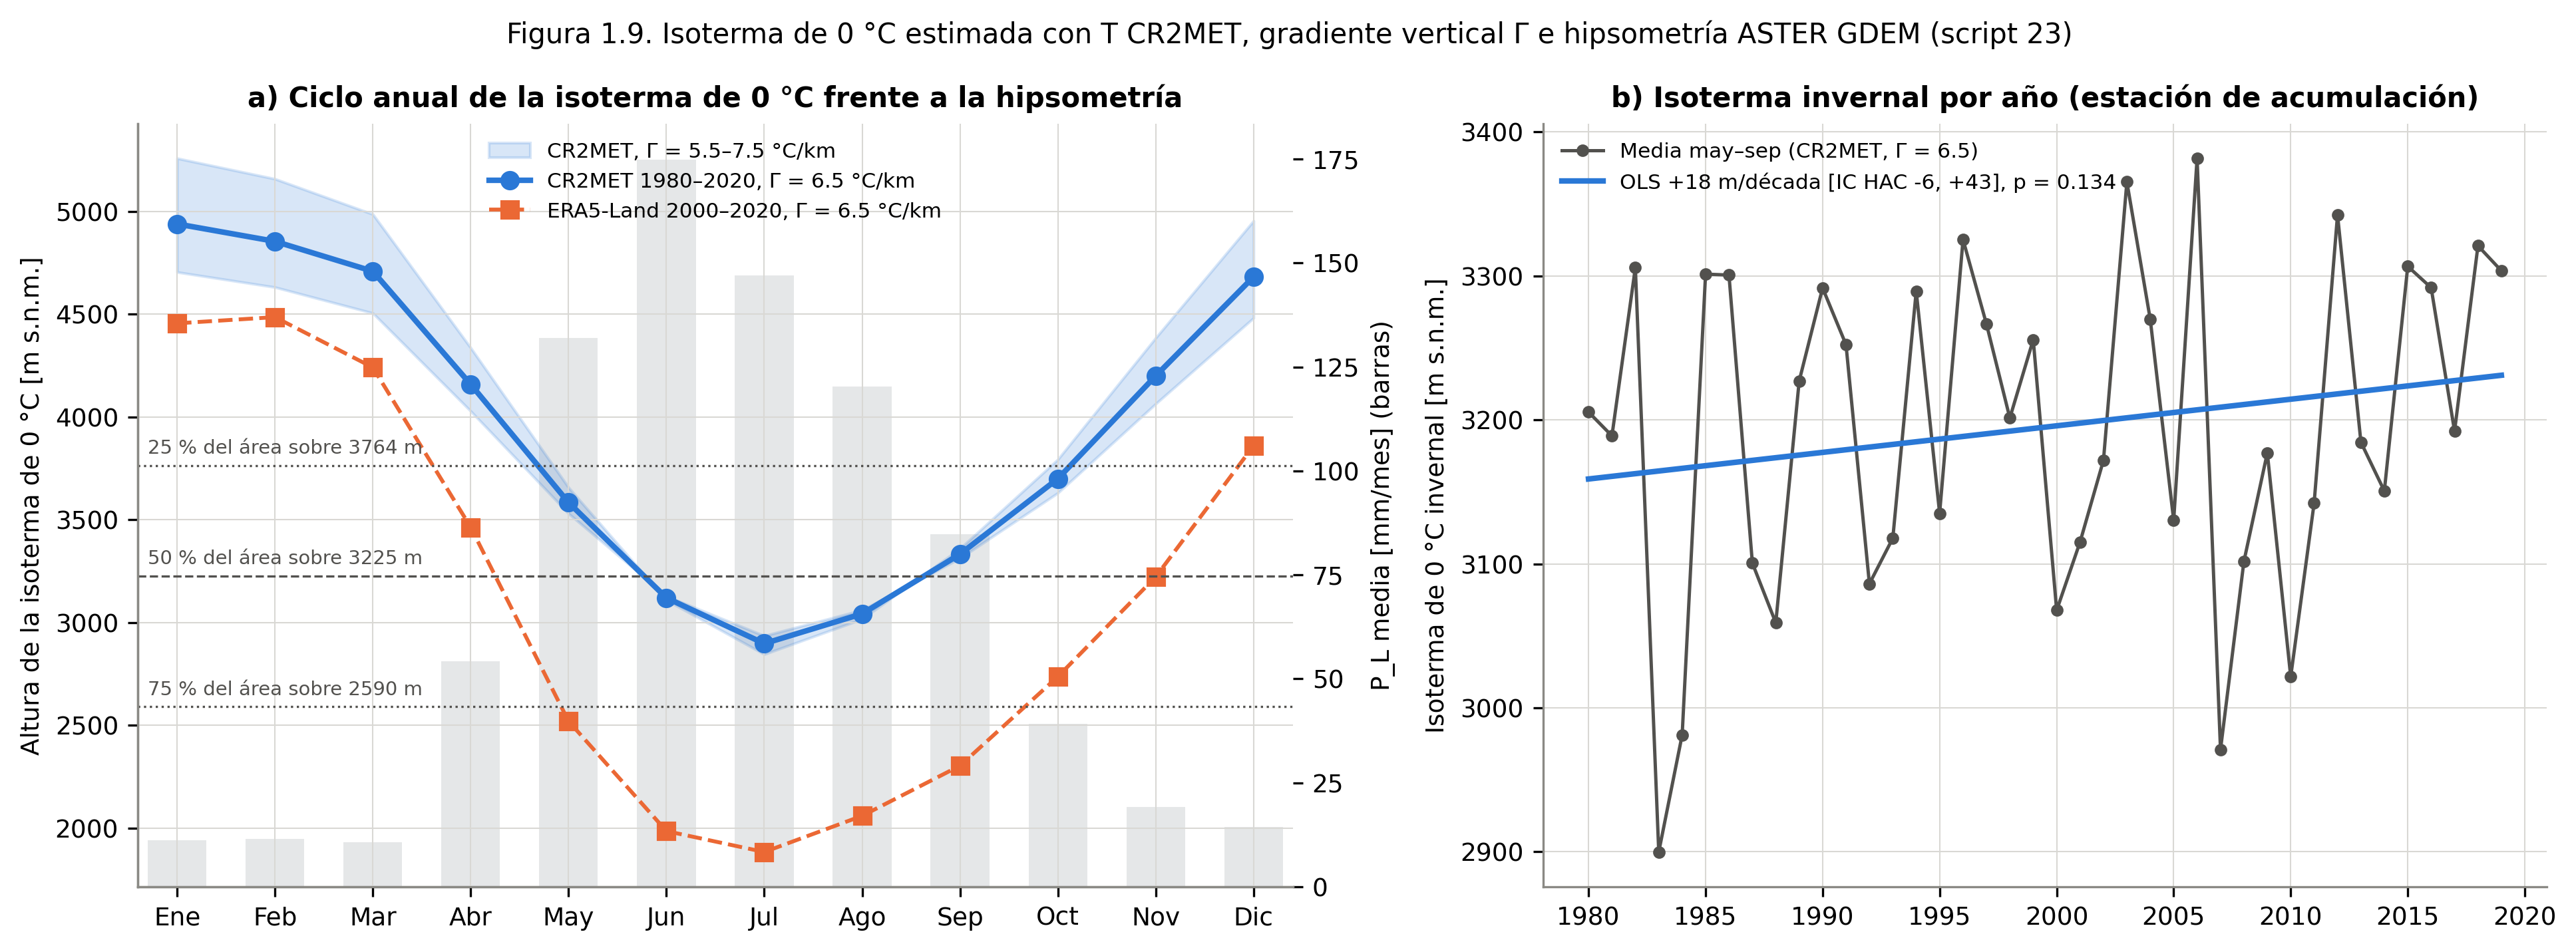
\includegraphics[width=\textwidth]{figura_1_9_isoterma_cero.png}
\caption{(a) Ciclo anual de la altura de la isoterma de 0~$^\circ$C estimada con la temperatura CR2MET (banda: $\Gamma$ de 5.5 a 7.5~$^\circ$C/km) y con ERA5-Land, frente a las elevaciones que dejan por encima el 25, 50 y 75\,\% del área; barras: $\PL$ media. (b) Isoterma media de mayo a septiembre por año y su tendencia OLS. Script \archivo{23_p1_5_isoterma_cero.py}.}
\label{fig:isoterma}
\end{figure}

\begin{purplebox}[title={Clasificación hidroclimática mensual (síntesis del punto 1)}]
\textbf{Régimen nival de montaña mediterránea, con almacenamiento estacional e interanual.} Criterios explícitos:
\begin{enumerate}[leftmargin=*]
\item \emph{Estacionalidad de la entrada}: precipitación unimodal invernal; mayo--agosto concentra el 70\,\% del total anual; $SI_P=0.75$ (``estacional''); máximo entre mayo y agosto en el 78\,\% de los años.
\item \emph{Estacionalidad de la salida, desfasada}: caudal unimodal con máximo en noviembre--enero en los 32 años completos y desfase de unos 6 meses respecto de la lluvia.
\item \emph{Fase nival}: de junio a agosto la isoterma de 0~$^\circ$C queda bajo la elevación mediana de la cuenca y entre el 46 y el 78\,\% de la precipitación cae sobre área bajo cero, según el producto de temperatura; 60\,\% del área sobre 3000~m.
\item \emph{Almacenamiento}: $SI_R=0.39$, CV del caudal de la mitad del de la lluvia, flujo base de 0.81, estiaje mínimo de 25~m$^3$/s y $R/P>1$ en 8 de 32 años, todos con lluvia anual bajo la media (1983 sigue al año récord de 1982).
\item \emph{Aridez}: el índice ETP/P de CAMELS-CL va de 0.75 (CR2MET) a 1.41 (MSWEP), por lo que la clase de aridez depende del producto. No asignamos una categoría de aridez; el rasgo robusto es la \emph{asincronía} entre lluvia (invierno) y energía (verano), propia del clima mediterráneo.
\end{enumerate}
\textbf{Hipótesis a contrastar}: (H-a) la lluvia mensual se relacionará con el caudal de varios meses después, no con el simultáneo (punto 2); (H-b) los cambios de la lluvia invernal se transmitirán al caudal de todo el año (punto 3); (H-c) el caudal tendrá un espectro más ``rojo'' que la lluvia (punto 4); (H-d) los modos que modulan la lluvia invernal se reflejarán en el caudal del verano siguiente (punto 5).
\end{purplebox}
\subsection{Punto 2. Relaciones entre series y modelos estadísticos}
\label{sec:p2}

\subsubsection{Diagramas de dispersión (2.1)}

\begin{figure}[H]
\centering
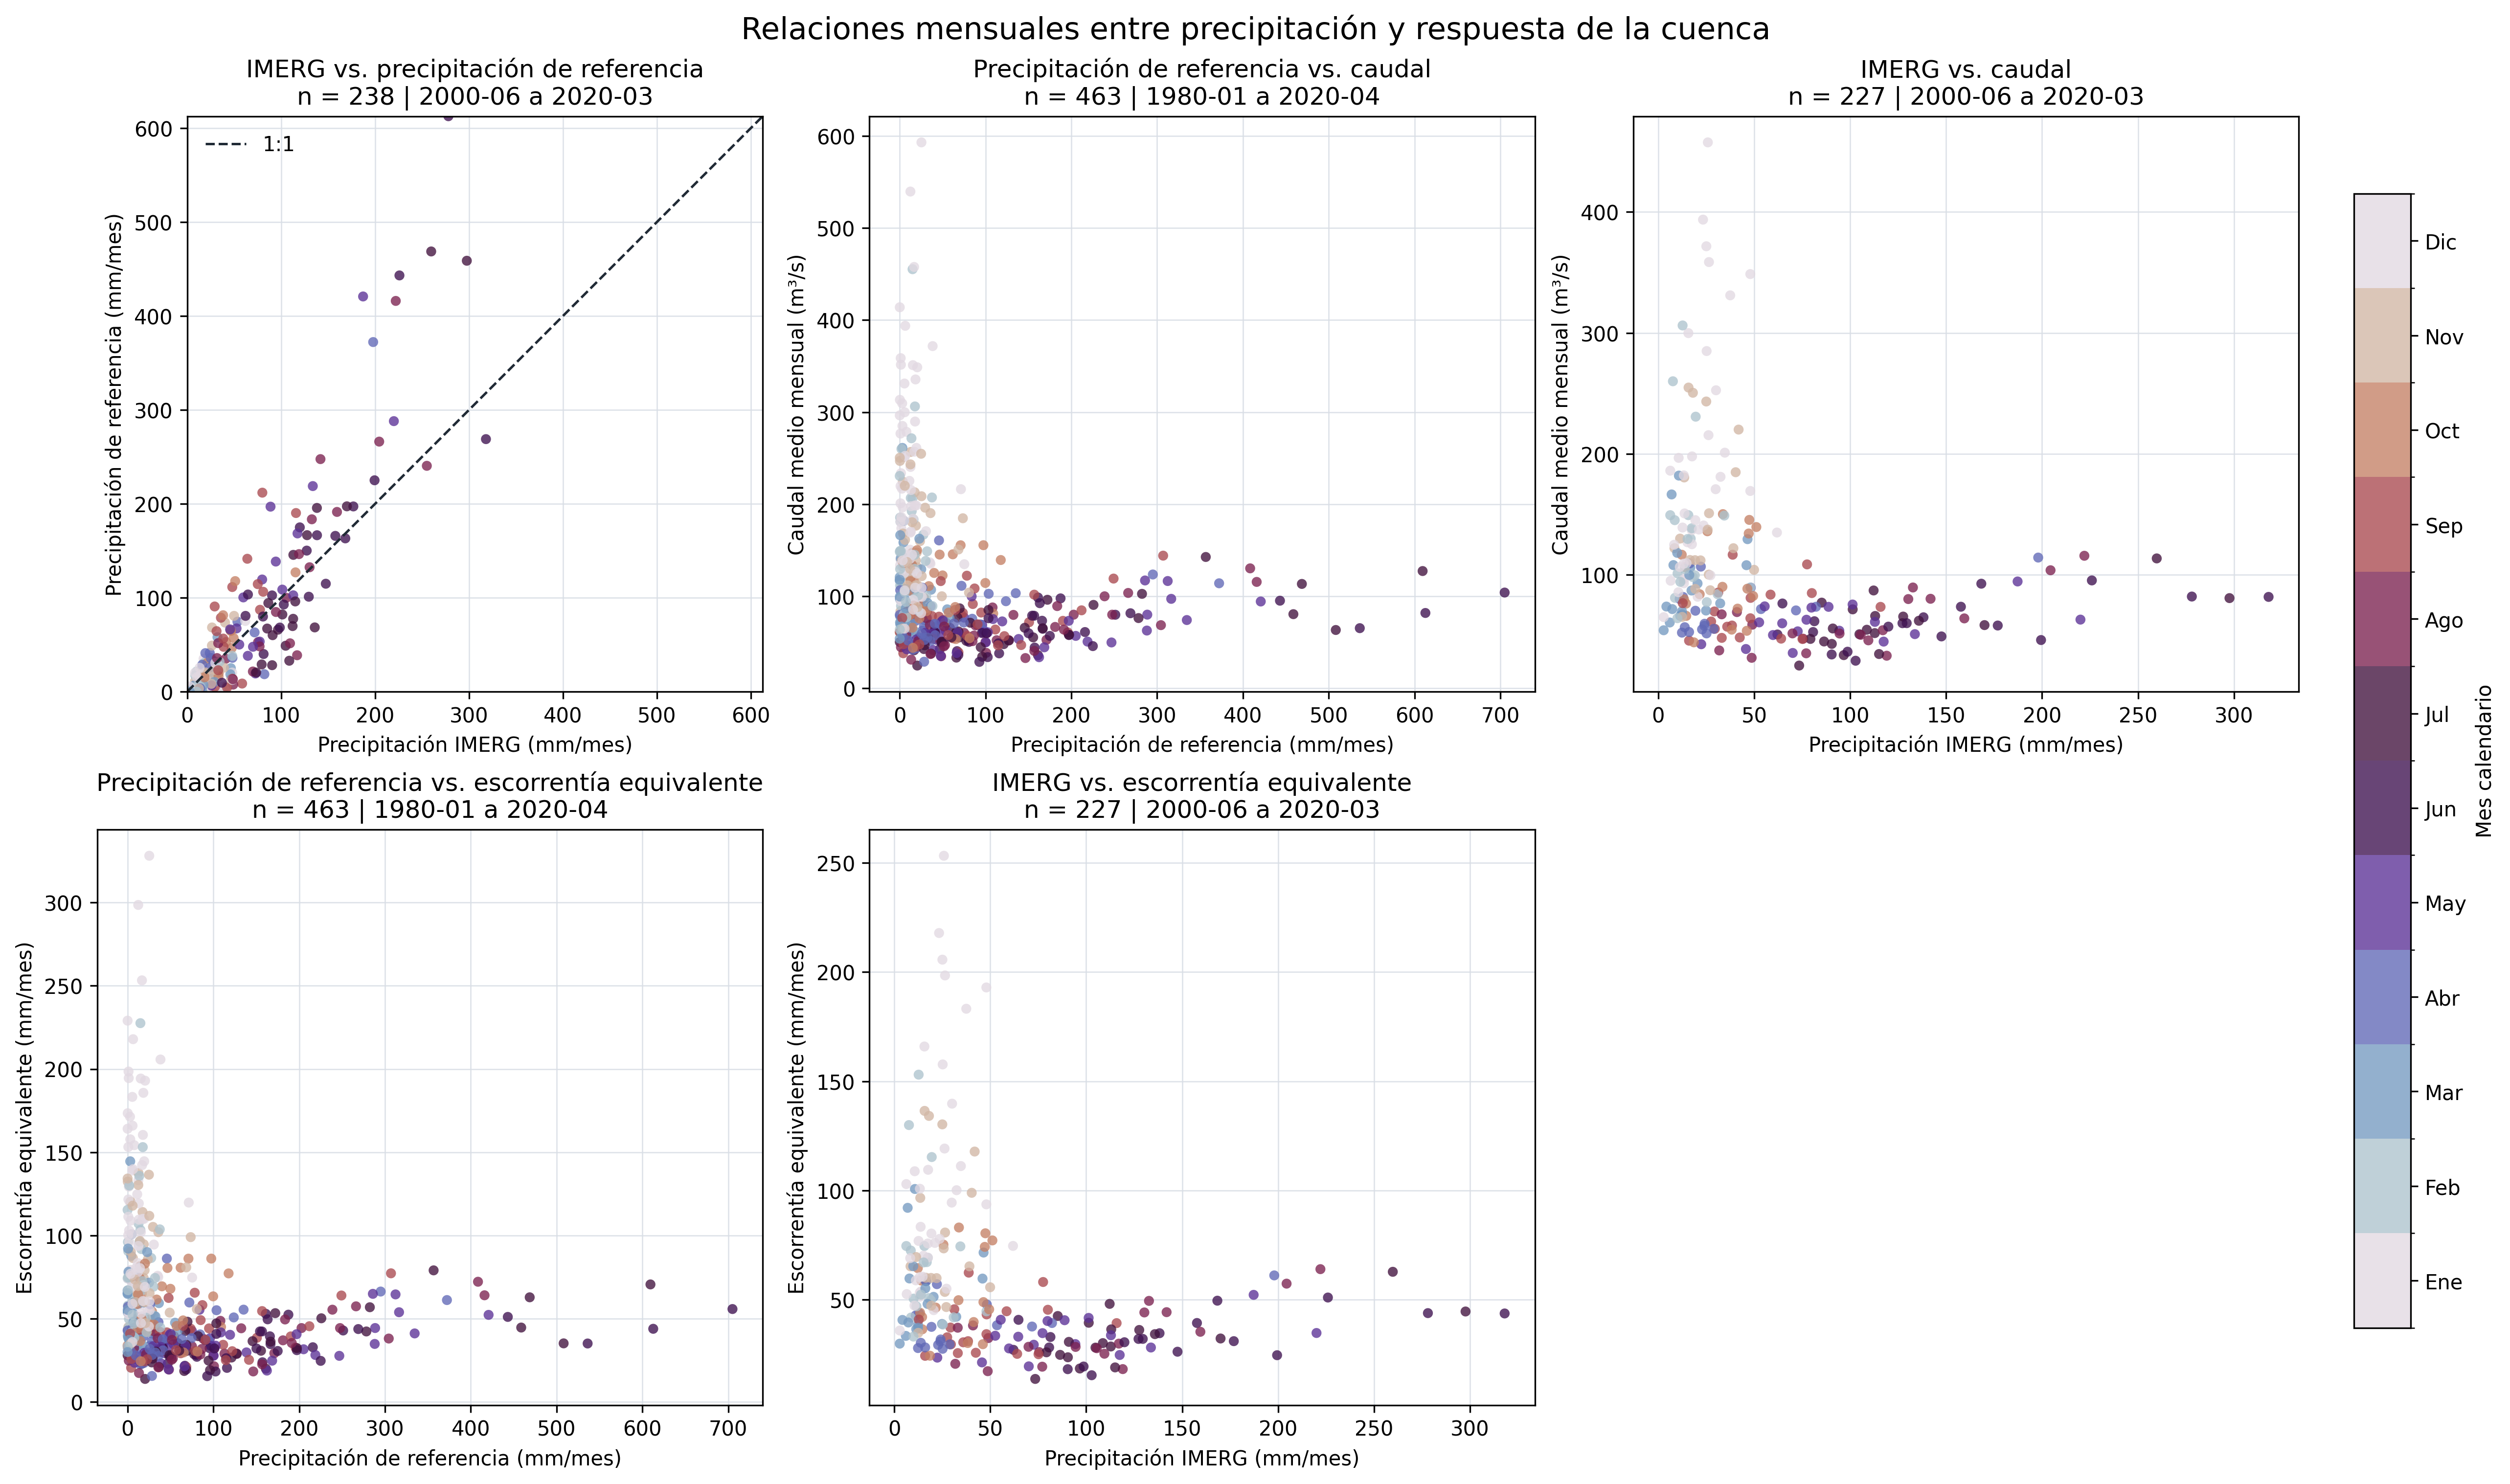
\includegraphics[width=\textwidth]{figura_2_1_relaciones_scatter.png}
\caption{Dispersión mensual de IMERG frente a la precipitación de referencia (con línea 1:1 y ejes comparables), de la precipitación local frente al caudal y de IMERG frente al caudal; colores por mes calendario. Ventanas y tamaños de muestra en cada panel. Script \archivo{04_analisis_precipitacion.py}.}
\label{fig:scatter}
\end{figure}

\begin{table}[H]
\centering\small
\caption{Asociación entre series mensuales con pares completos (\archivo{figuras/tabla_2_1_metricas_relaciones.csv}) y correlación de anomalías sin rezago (\archivo{figuras/tabla_2_2_correlaciones_rezagos.csv}).}
\label{tab:relaciones}
\begin{tabular}{llrrrr}
\toprule
Par & Periodo & $n$ & Pearson $r$ & Spearman $\rho$ & $r$ de anomalías \\
\midrule
$\PI$--$\PL$ & 2000-06 a 2020-03 & 238 & 0.888 & 0.824 & -- \\
$\PL$--$\Qm$ & 1980-01 a 2020-04 & 463 & $-0.217$ & $-0.401$ & 0.140 \\
$\PI$--$\Qm$ & 2000-06 a 2020-03 & 227 & $-0.277$ & $-0.421$ & 0.180 \\
$\PL$--$R$ & 1980-01 a 2020-04 & 463 & $-0.213$ & $-0.395$ & -- \\
$\PI$--$R$ & 2000-06 a 2020-03 & 227 & $-0.270$ & $-0.412$ & -- \\
\bottomrule
\end{tabular}
\end{table}

\paragraph{IMERG frente a la referencia.} En los 238 pares, la asociación es alta ($r=0.888$; $\rho=0.824$), pero la concordancia es imperfecta: sesgo medio $\PI-\PL=-5.50$~mm/mes, MAE de 27.3~mm/mes, RMSE de 48.7~mm/mes y PBIAS de $-8.8$\,\%. El signo medio no describe cada mes: IMERG está por debajo en 103 pares y por encima en 135, y la mediana del error es $+3.9$~mm/mes. El error depende de la estación y de la intensidad (Tabla~\ref{tab:errgrupo}): en verano IMERG sobreestima ($+6.9$~mm/mes) y en invierno subestima ($-11.3$~mm/mes), y en el cuartil más lluvioso el sesgo llega a $-51.9$~mm/mes con un RMSE de 88.5~mm/mes. Los cinco meses con mayor error, todos de invierno (2000-06, 2008-05, 2005-06, 2006-07 y 2005-08, con errores de $-194$ a $-335$~mm/mes), reúnen el 52\,\% del error cuadrático. Sin ellos, Pearson casi no cambia (0.883) pero el RMSE baja a 33.9~mm/mes. Que Spearman sea menor que Pearson indica que el orden de los meses secos concuerda peor que la magnitud de los meses lluviosos, coherente con que IMERG nunca registre cero.

\begin{table}[H]
\centering\small
\caption{Error de IMERG por estación austral y por cuartil de $\PL$ (\archivo{figuras/tabla_2_1_errores_por_grupo.csv}); mm/mes.}
\label{tab:errgrupo}
\begin{tabular}{llrrrr}
\toprule
Grupo & Clase & $n$ & Sesgo & MAE & RMSE \\
\midrule
Estación & Verano (DEF) & 60 & $+6.85$ & 11.26 & 14.20 \\
 & Otoño (MAM) & 58 & $-9.38$ & 26.12 & 47.76 \\
 & Invierno (JJA) & 60 & $-11.33$ & 49.10 & 76.72 \\
 & Primavera (SON) & 60 & $-8.28$ & 22.85 & 33.13 \\
Cuartil de $\PL$ & Q1 (0--8.5) & 60 & $+14.00$ & 14.09 & 17.06 \\
 & Q2 (8.5--25.6) & 59 & $+9.97$ & 13.49 & 20.54 \\
 & Q3 (25.6--78.5) & 59 & $+6.43$ & 22.74 & 29.39 \\
 & Q4 (78.5--612.7) & 60 & $-51.94$ & 58.75 & 88.52 \\
\bottomrule
\end{tabular}
\end{table}

\begin{razonamiento}{Mecanismo y alternativas del error de IMERG}
\textbf{Resultado}: IMERG atenúa los extremos (sobreestima meses secos y subestima los muy lluviosos). \textbf{Mecanismo propuesto}: la precipitación invernal intensa de la cuenca es en gran parte orográfica y cae como nieve sobre terreno complejo; los sensores de microondas y los algoritmos de IMERG tienen dificultades para estimar la precipitación sólida y el realce orográfico de capas poco profundas, y el ajuste con pluviómetros mensuales depende de una red escasa en altura \citep{Rojas2021,Tian2018,Zambrano2017}. \textbf{Alternativa}: CR2MET podría sobreestimar los inviernos extremos, porque también es una estimación. Distinguirlas exigiría pluviómetros de altura independientes o la nieve acumulada. Las dos fuentes comparten información de pluviómetros, por lo que su concordancia no es una validación independiente.
\end{razonamiento}

\paragraph{Precipitación frente a caudal.} En las series originales, la correlación lluvia--caudal es \emph{negativa} ($r=-0.22$; $\rho=-0.40$): el caudal es alto en verano, cuando no llueve, y bajo en invierno, cuando llueve. Es el ciclo anual compartido, en oposición de fase, el que domina la asociación. Al retirar la climatología mensual, la correlación contemporánea se vuelve débilmente positiva (0.14 para $\PL$ y 0.18 para IMERG). Las dos cifras responden preguntas distintas y no se contradicen. El uso de $R$ en lugar de $\Qm$ no cambia la lectura (Tabla~\ref{tab:relaciones}), porque $R$ es una transformación casi lineal de $\Qm$.

\paragraph{Rezagos.} Con lluvia en $t-k$ y caudal en $t$, la correlación de anomalías crece con el rezago hasta un máximo en $k=7$ meses ($r=0.493$ con $\PL$, $n=456$; $r=0.428$ con IMERG, $n=221$) y decae a cero hacia $k=12$ (Figura~\ref{fig:rezagos2}). Es el comportamiento esperado si la lluvia de invierno sale como caudal en primavera--verano. Sin embargo, el máximo surge de una búsqueda entre 13 rezagos en series autocorrelacionadas, por lo que no lo interpretamos como un tiempo físico de deshielo ni le asignamos significancia \citep{PyperPeterman1998}.

\begin{figure}[H]
\centering
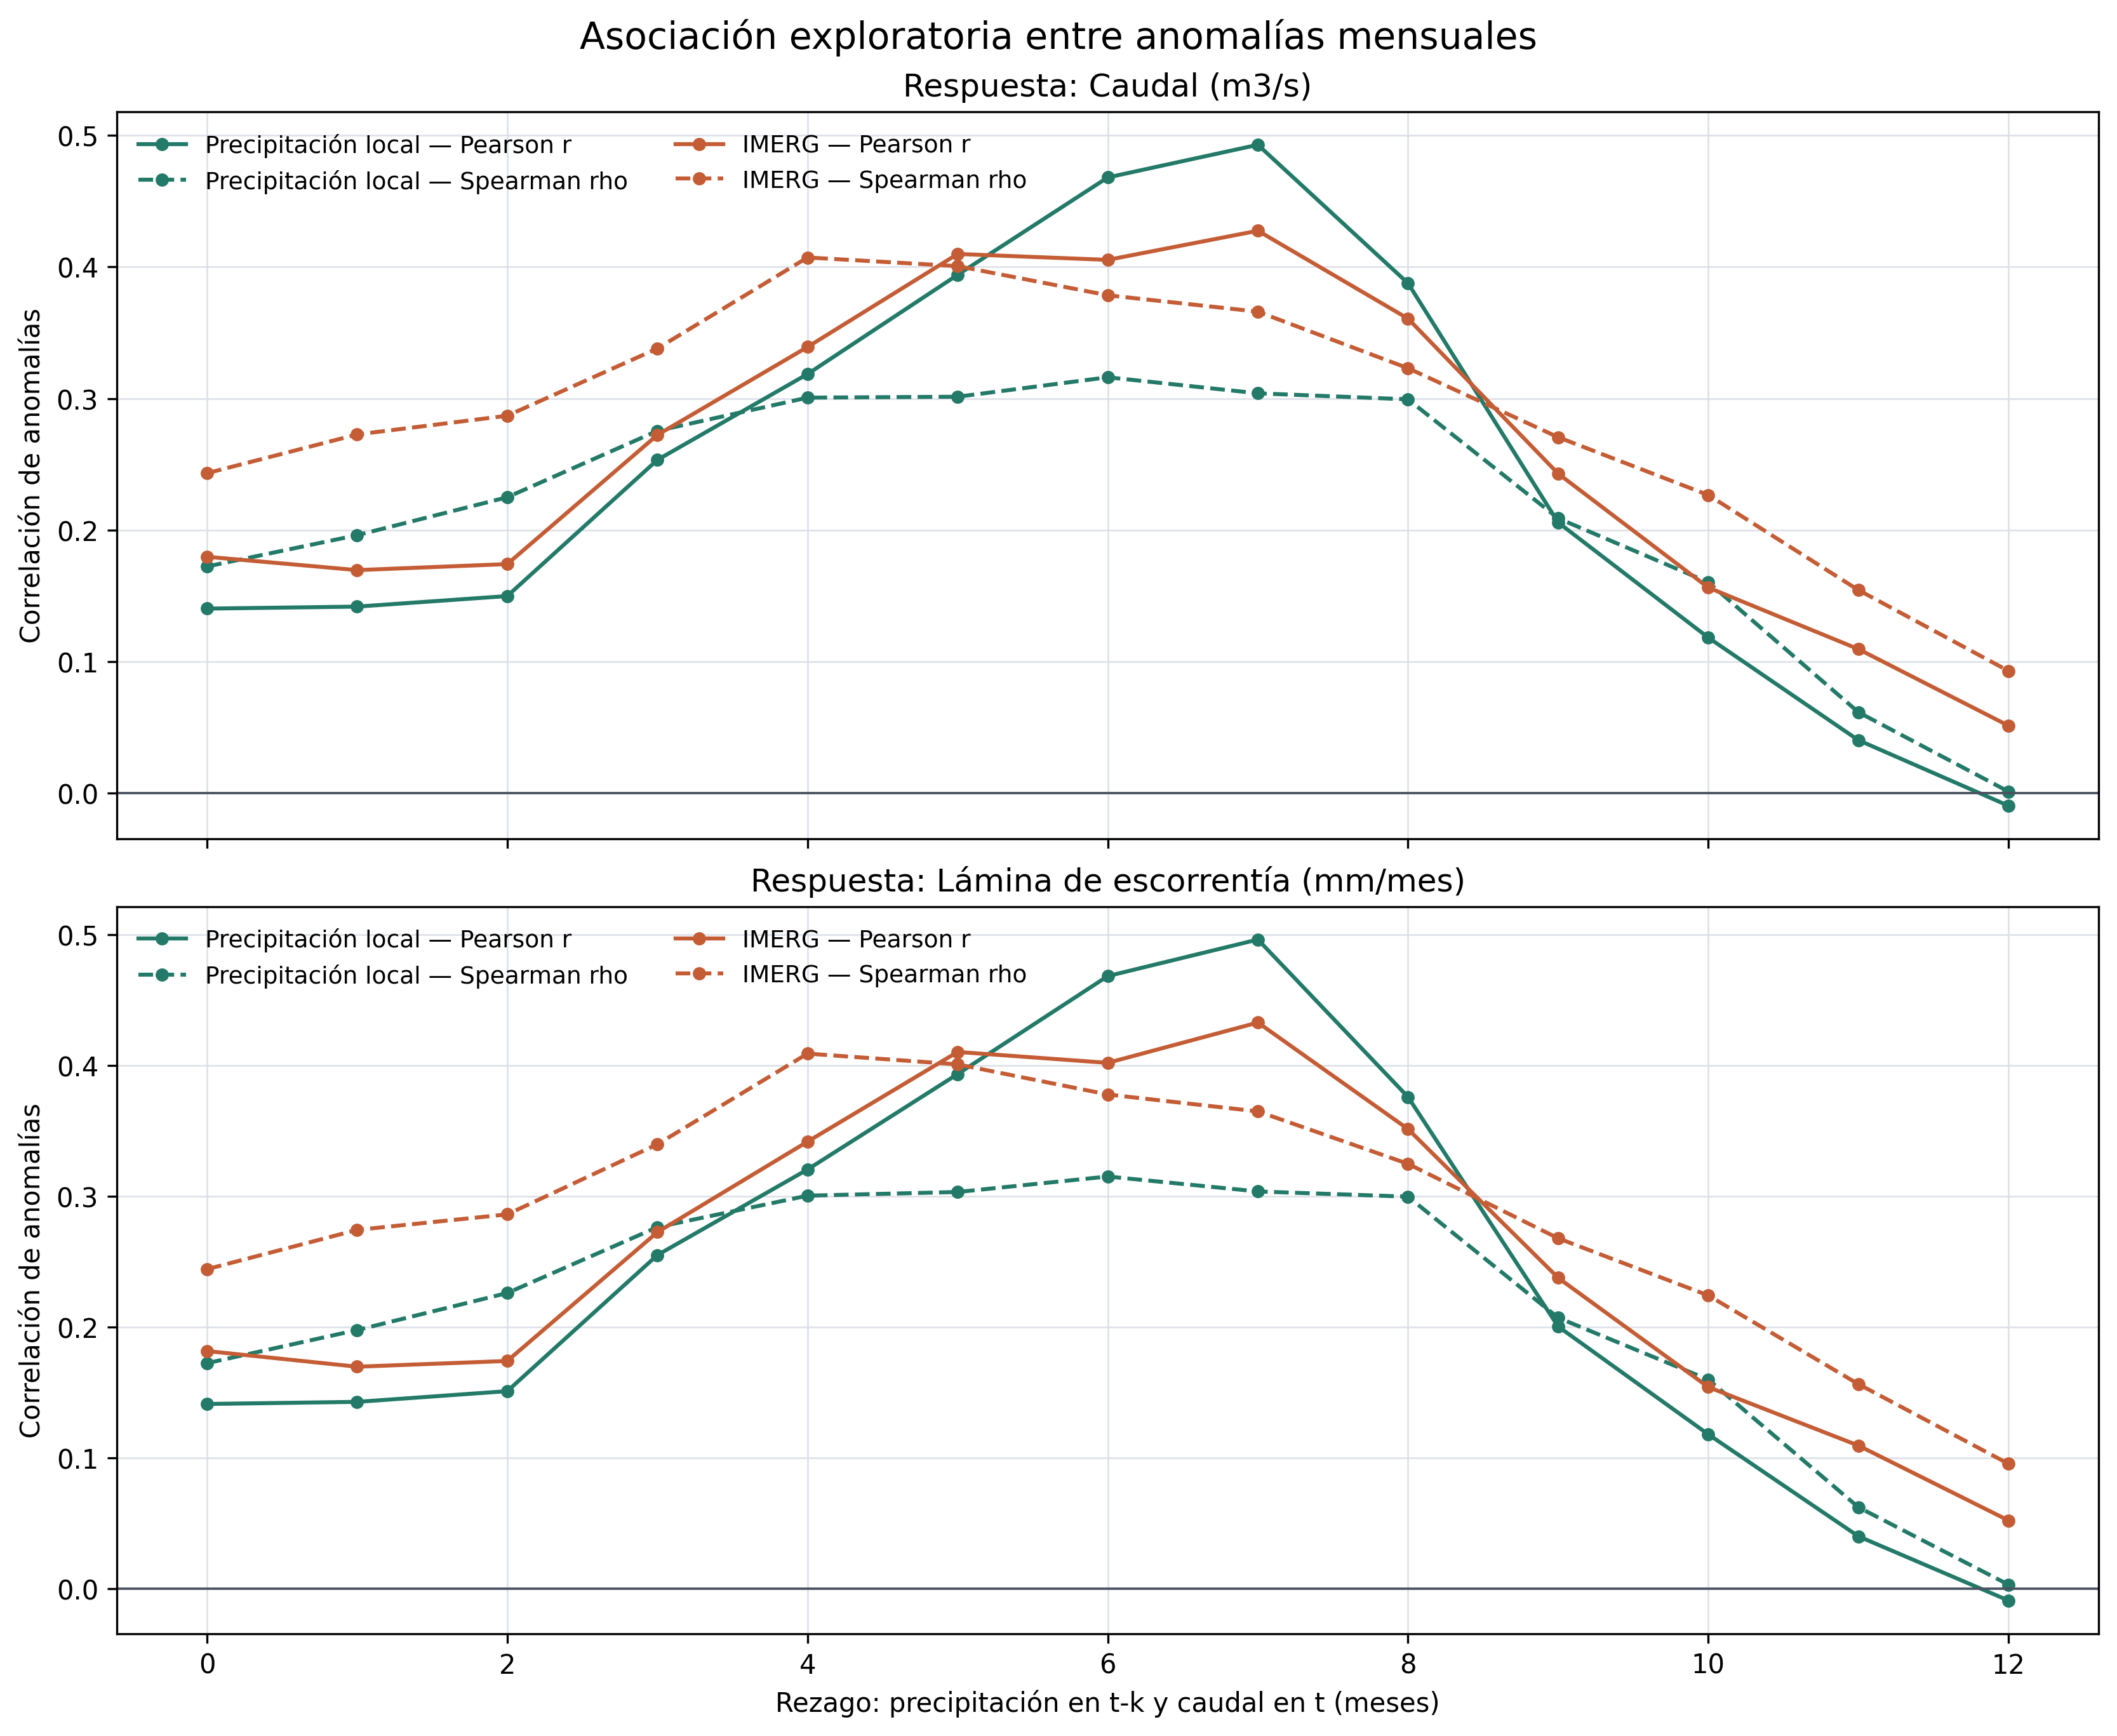
\includegraphics[width=0.78\textwidth]{figura_2_2_correlaciones_rezagos.png}
\caption{Correlación de Pearson y Spearman entre la anomalía de precipitación en $t-k$ y la anomalía de caudal en $t$, para la referencia e IMERG. Exploratorio: no se ajustó por dependencia ni por la búsqueda entre rezagos. Script \archivo{05_anomalias_rezagos.py}.}
\label{fig:rezagos2}
\end{figure}

\subsubsection{Modelos y evaluación fuera del ajuste (2.2 y 2.3)}

\paragraph{Modelos.} Para la lluvia local probamos una corrección lineal de IMERG y otra log-lineal. Para el caudal comparamos la climatología mensual, una regresión contemporánea $\Qm\sim P(t)$ y el modelo de anomalías con rezago (Ecuación~\ref{eq:modeloq}). Este último suma a la climatología del caudal un término proporcional a la anomalía de lluvia $k$ meses antes. Es una relación empírica de predicción: no conserva masa ni representa la evapotranspiración, la nieve o la regulación. Su dominio de aplicación es el de las anomalías observadas en el ajuste, y sus unidades son m$^3$/s para el caudal y mm/mes para la lluvia. Las predicciones de lluvia negativas se truncan a cero; las de caudal nunca fueron negativas.

\begin{table}[H]
\centering\small
\caption{Errores fuera del ajuste en los tres bloques externos (\archivo{figuras/tabla_2_3_metricas_por_bloque.csv} y \archivo{figuras/tabla_2_3_seleccion_modelos_ajuste.csv}). MAE/RMSE en mm/mes para la lluvia y en m$^3$/s para el caudal; $k$ es el rezago elegido dentro del ajuste. Sesgo = predicción $-$ observado.}
\label{tab:bloques}
\begin{tabular}{llrrrrrr}
\toprule
Objetivo & Bloque & $n$ & $k$ & Referencia & Lineal & Anomalía rezagada & Sesgo rezago \\
\midrule
$\PL$ desde $\PI$ & 2010--12 & 36 & -- & 17.3/23.5 & 21.9/31.8 & -- & -- \\
 & 2013--15 & 36 & -- & 19.0/25.1 & 22.5/38.0 & -- & -- \\
 & 2016--20 & 51 & -- & 18.8/32.6 & 20.9/30.7 & -- & -- \\
$\Qm$ desde $\PL$ & 2010--12 & 36 & 6 & 49.9/64.6 & 60.4/65.2 & \textbf{42.2/54.3} & 41.9 \\
 & 2013--15 & 26 & 7 & 48.1/59.3 & 48.8/53.7 & \textbf{38.8/49.5} & 38.7 \\
 & 2016--20 & 51 & 6 & 42.1/54.9 & 51.4/56.7 & \textbf{37.3/46.7} & 34.9 \\
$\Qm$ desde $\PI$ & 2010--12 & 36 & 7 & 49.9/64.6 & 66.2/71.0 & \textbf{44.4/55.9} & 44.4 \\
 & 2013--15 & 26 & 7 & 48.1/59.3 & 46.7/51.0 & \textbf{34.0/46.7} & 34.0 \\
 & 2016--20 & 51 & 7 & 42.1/54.9 & 47.1/52.0 & \textbf{35.9/47.4} & 26.5 \\
\bottomrule
\end{tabular}
\end{table}

\paragraph{Resultados.} (i) Corregir IMERG \emph{no} mejora la estimación de la lluvia local: con las predicciones de los tres bloques agregadas, el MAE sube de 18.4 a 21.7~mm/mes y el RMSE de 28.1 a 33.3~mm/mes. IMERG sin corregir es preferible. (ii) Para el caudal, el modelo de anomalías con rezago reduce el MAE y el RMSE frente a la climatología en los tres bloques y para las dos fuentes de lluvia (agregado con $\PL$: MAE de 46.0 a 39.2~m$^3$/s y RMSE de 59.2 a 49.8~m$^3$/s; con IMERG, MAE de 46.0 a 38.1 y RMSE de 59.2 a 50.1). La regresión contemporánea es peor que la climatología, coherente con la correlación negativa del ciclo anual. (iii) Todos los modelos de caudal tienen un \emph{sesgo positivo} de 26--50~m$^3$/s: entrenados con años más húmedos, sobreestiman el caudal de la megasequía, lo que anticipa la tendencia del punto 3. (iv) El rezago elegido dentro de cada ajuste es estable: 6--7 meses con $\PL$ y 7 meses con IMERG.

\begin{figure}[H]
\centering
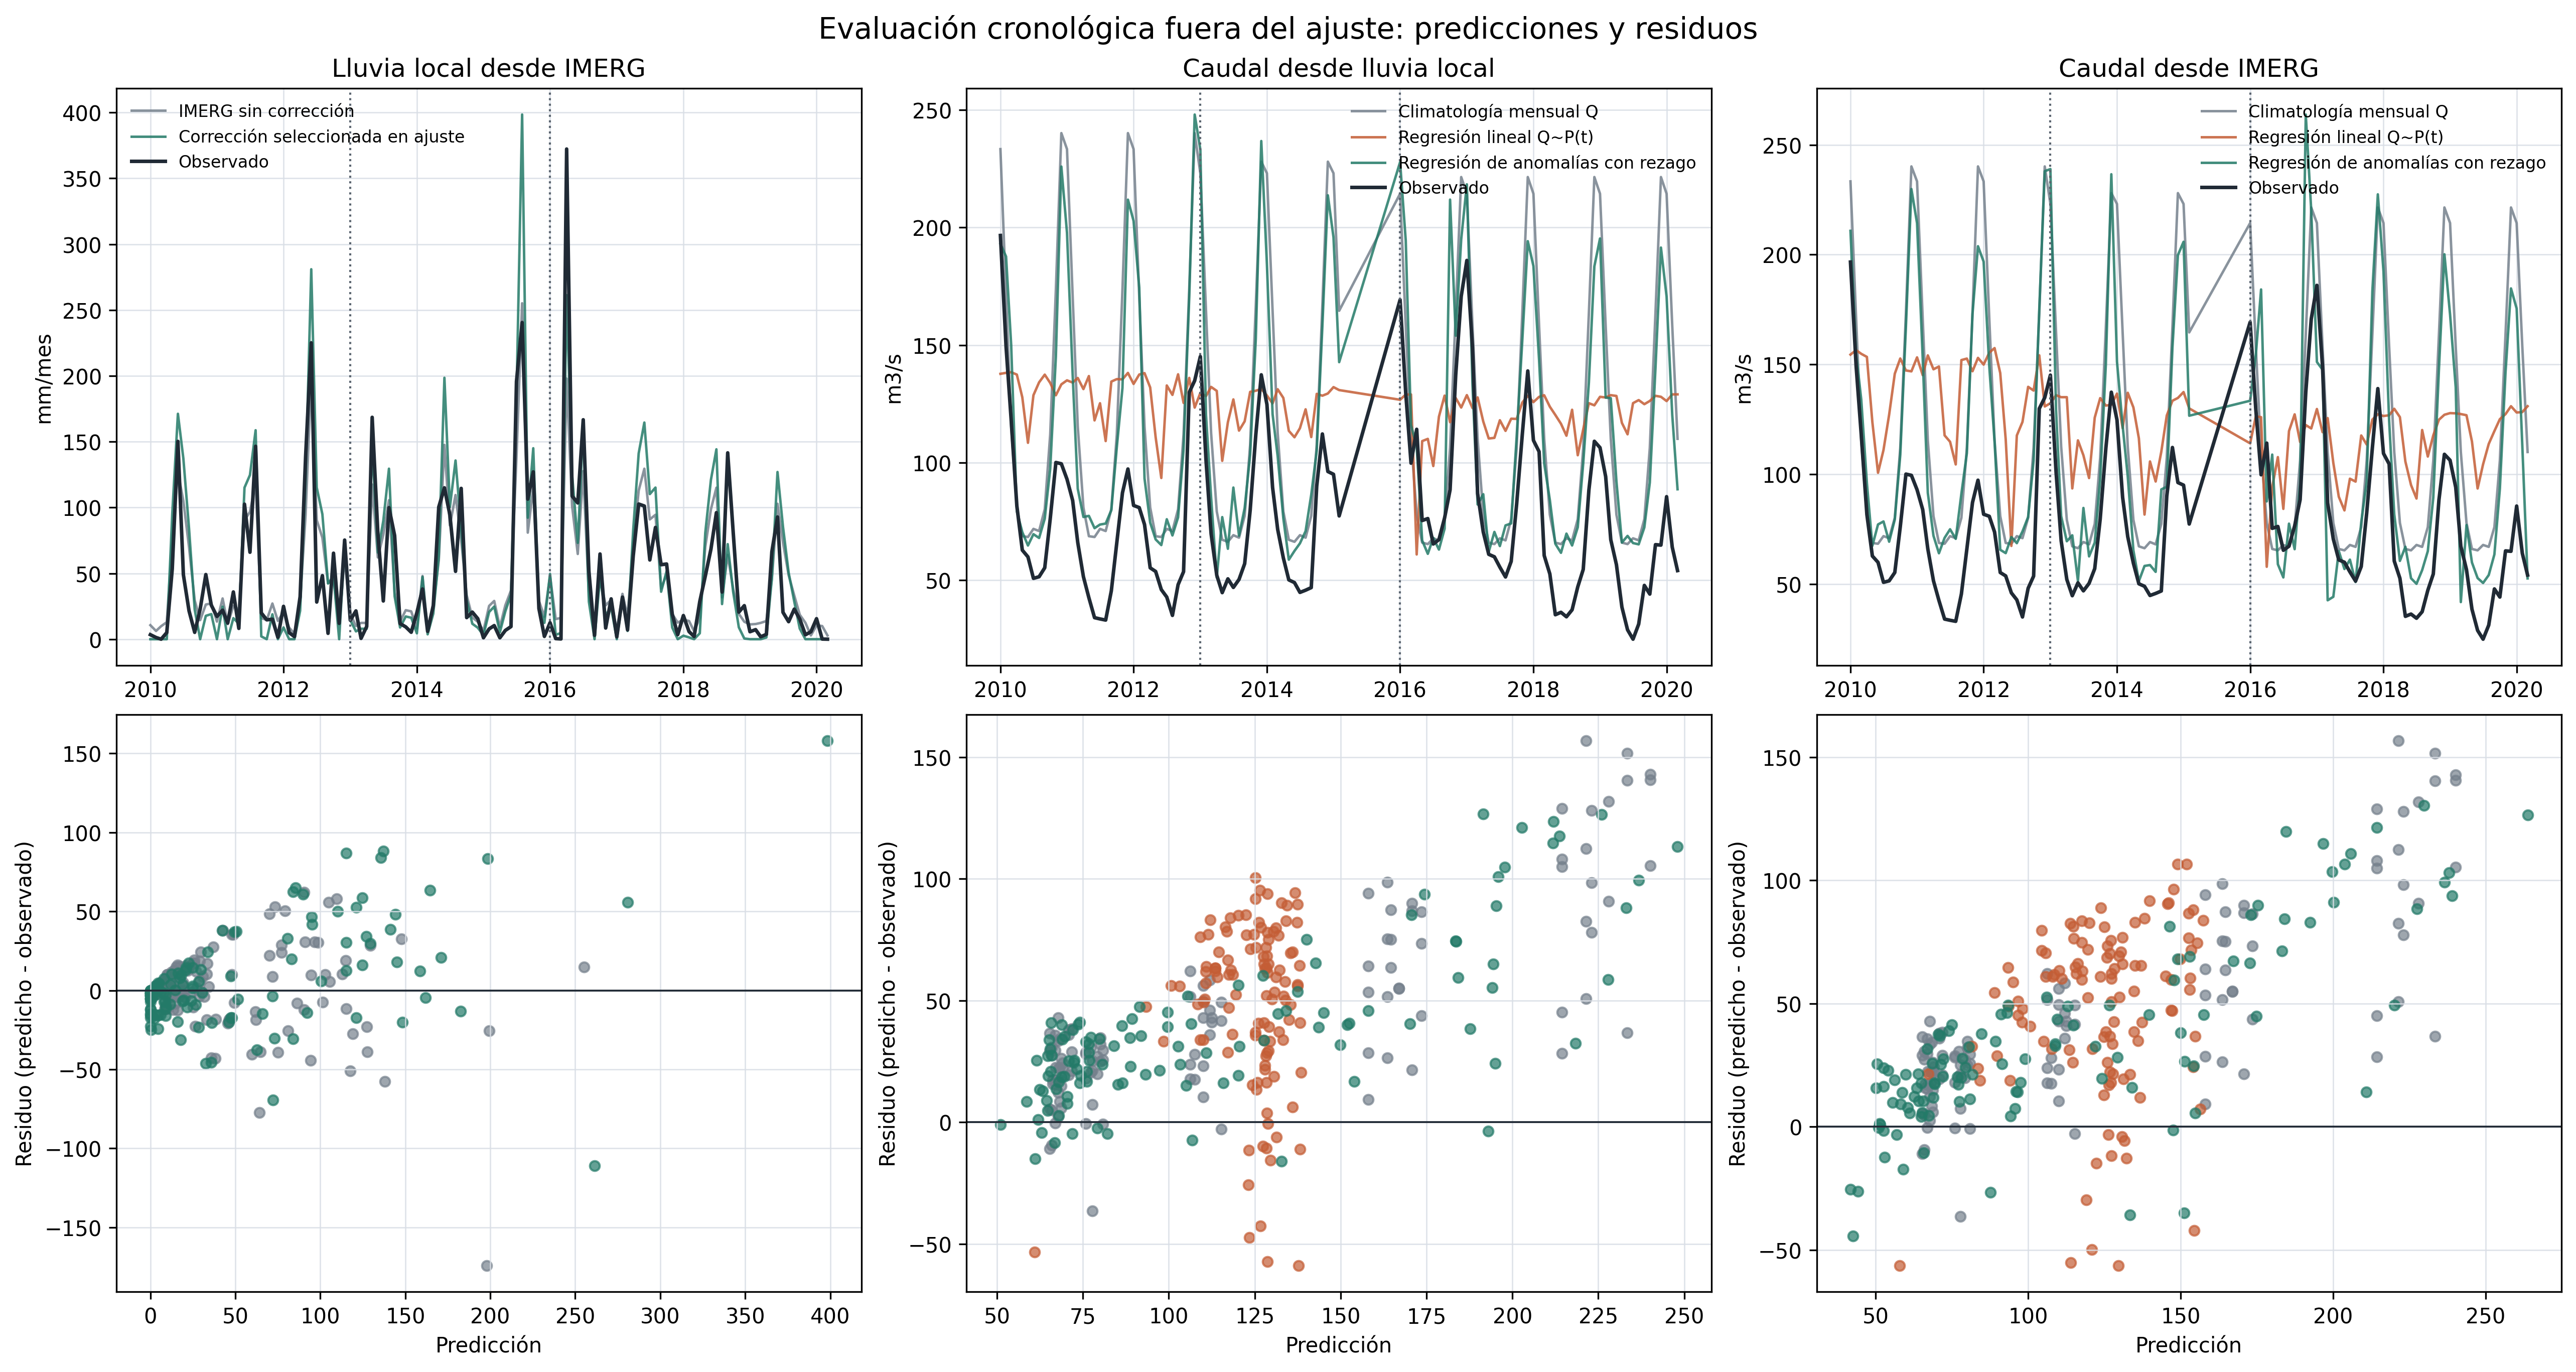
\includegraphics[width=\textwidth]{figura_2_3_validacion_modelos.png}
\caption{Predicciones fuera del ajuste en los tres bloques y residuos frente al valor estimado. Script \archivo{06_modelos_validacion_temporal.py}.}
\label{fig:validacion}
\end{figure}

\paragraph{Diagnóstico.} Los errores del modelo rezagado con $\PL$ se concentran en el deshielo: el MAE es de 44--95~m$^3$/s de octubre a enero y de 17--28~m$^3$/s de marzo a septiembre, casi todo como sesgo positivo (cálculo por mes a partir de \archivo{figuras/tabla_2_3_residuos_por_mes.csv}). Es la estación con mayor varianza entre años y la más afectada por la megasequía. Las mayores sobreestimaciones ocurren en el deshielo de años secos, como diciembre de 2019 (191.5~m$^3$/s predichos frente a 64.8 observados con $\PL$) y diciembre de 2010 (225.9 frente a 99.5). Son errores de eventos concretos, no predicciones físicamente imposibles: quedan dentro del rango histórico del ajuste, pero superan el máximo del bloque evaluado (\archivo{figuras/tabla_2_3_maximos_predichos.csv}). Los bloques no son réplicas independientes, porque el entrenamiento se amplía de un bloque al siguiente.

\begin{purplebox}[title={Conclusión del punto 2}]
\textbf{¿Existe una relación aprovechable?} Sí, para el caudal, y es \emph{retardada}: la anomalía de lluvia de unos 6--7 meses antes mejora la estimación del caudal frente a la climatología en las tres ventanas evaluadas, para las dos fuentes de lluvia. Es la huella estadística del almacenamiento nival (hipótesis H-a del punto 1), aunque el rezago óptimo no es un tiempo físico medido. \textbf{¿Para qué condiciones?} Mejor en primavera--verano, con sesgo positivo persistente durante la megasequía. \textbf{Lluvia local desde IMERG}: la corrección estadística no mejora a IMERG crudo; el producto es útil para el ciclo y la variabilidad, pero subestima los inviernos intensos. Es una evidencia retrospectiva que no garantiza capacidad de pronóstico futuro.
\end{purplebox}
\subsection{Punto 3. Tendencias hidroclimáticas y sus posibles causas}
\label{sec:p3}

\subsubsection{Temperatura, periodos y representaciones (3.1 y 3.2)}

Los periodos, la cobertura y la referencia se describieron en las Secciones~\ref{sec:datos} y \ref{sec:anomalias}. $\PL$, $\Qm$ y $T$ (CR2MET) se analizan en su registro completo de 40 años y $\PI$ en sus 20 años; la temperatura ERA5-Land se usa como contraste en sus 20 años. Las cuatro variables se comparan además en el periodo común, sin rellenar faltantes y sin unir fuentes distintas en una sola serie. La lámina $R$ no se analiza por separado, porque es una transformación casi lineal de $\Qm$ y no aporta evidencia independiente. La Figura~\ref{fig:rep} presenta las tres representaciones. $X$ conserva el ciclo anual y las unidades; $a$ retira el ciclo y conserva las unidades; $z$ es adimensional y da el mismo peso a cada mes. Por eso $z$ amplifica las desviaciones de los meses casi secos: en $\PL$, marzo, abril, julio y diciembre tienen $s_j/\mu_j>1$. Con el criterio de completitud, el mayor $|z|$ del registro es 5.0 (caudal); el valor de 16.5 que producía el mayo de 1993 incompleto desapareció (Sección~\ref{sec:qc}).

\begin{figure}[H]
\centering
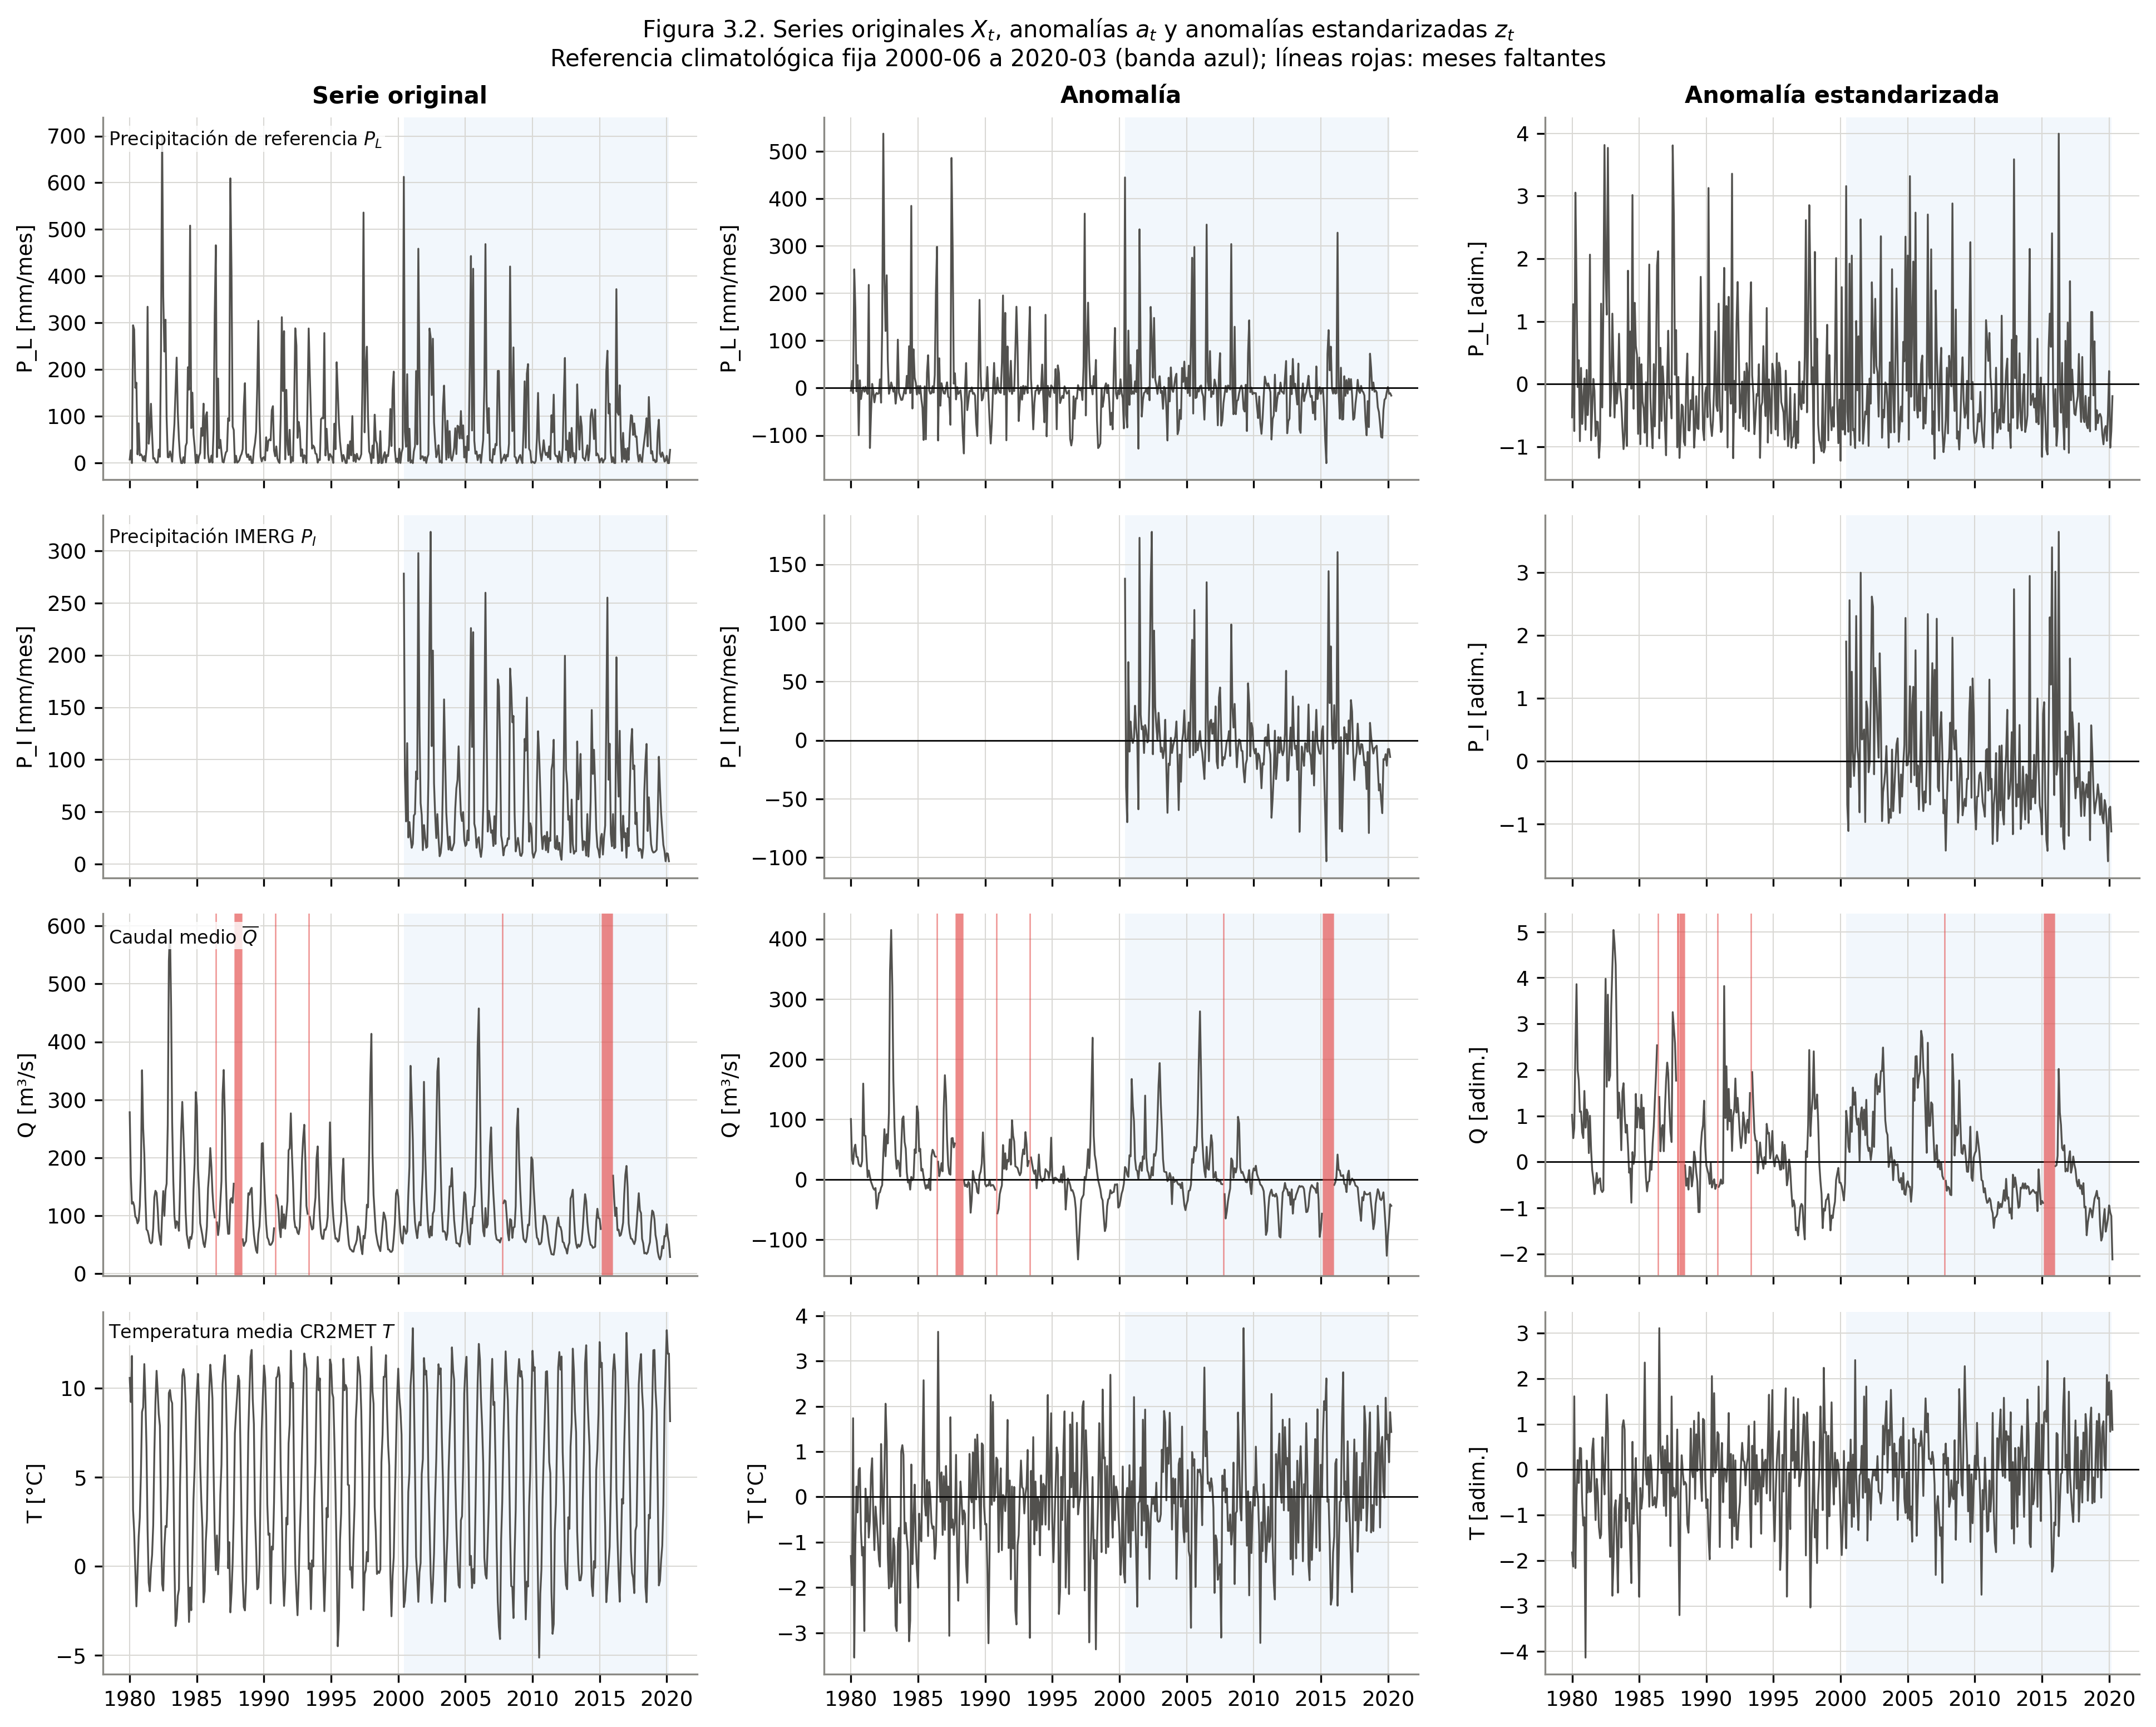
\includegraphics[width=0.95\textwidth]{figura_3_2_representaciones.png}
\caption{Series originales $X_t$, anomalías $a_t$ y anomalías estandarizadas $z_t$. Banda azul: referencia 2000-06 a 2020-03; líneas rojas: meses faltantes, no rellenados. Script \archivo{09_p3_2_anomalias.py}.}
\label{fig:rep}
\end{figure}

\subsubsection{Dos escalas de evaluación (3.3)}

Verificamos numéricamente que, dentro de un mismo mes calendario y con la misma muestra, la pendiente OLS de $a$ es idéntica a la de $X$ y la de $z$ es la de $X$ dividida por $s_j$ (diferencia máxima de $2.1\times10^{-14}$; \archivo{figuras/tabla_3_3_verificacion_invarianza.csv}). Mes a mes, por lo tanto, $X$, $a$ y $z$ \emph{no} son evidencias independientes de tendencia. A escala global sí difieren: OLS sobre $X$ está afectada por la fase del ciclo en los extremos del registro, y $z$ pondera igual meses secos y húmedos. Un ejemplo: la OLS simple de $\PI$ sobre $X$ da $-18.1$~mm/mes por década porque el registro empieza en el invierno lluvioso (junio de 2000) y termina en el verano seco (marzo de 2020); con efectos de mes la pendiente es de $-15.6$, igual a la de las anomalías.

\begin{figure}[H]
\centering
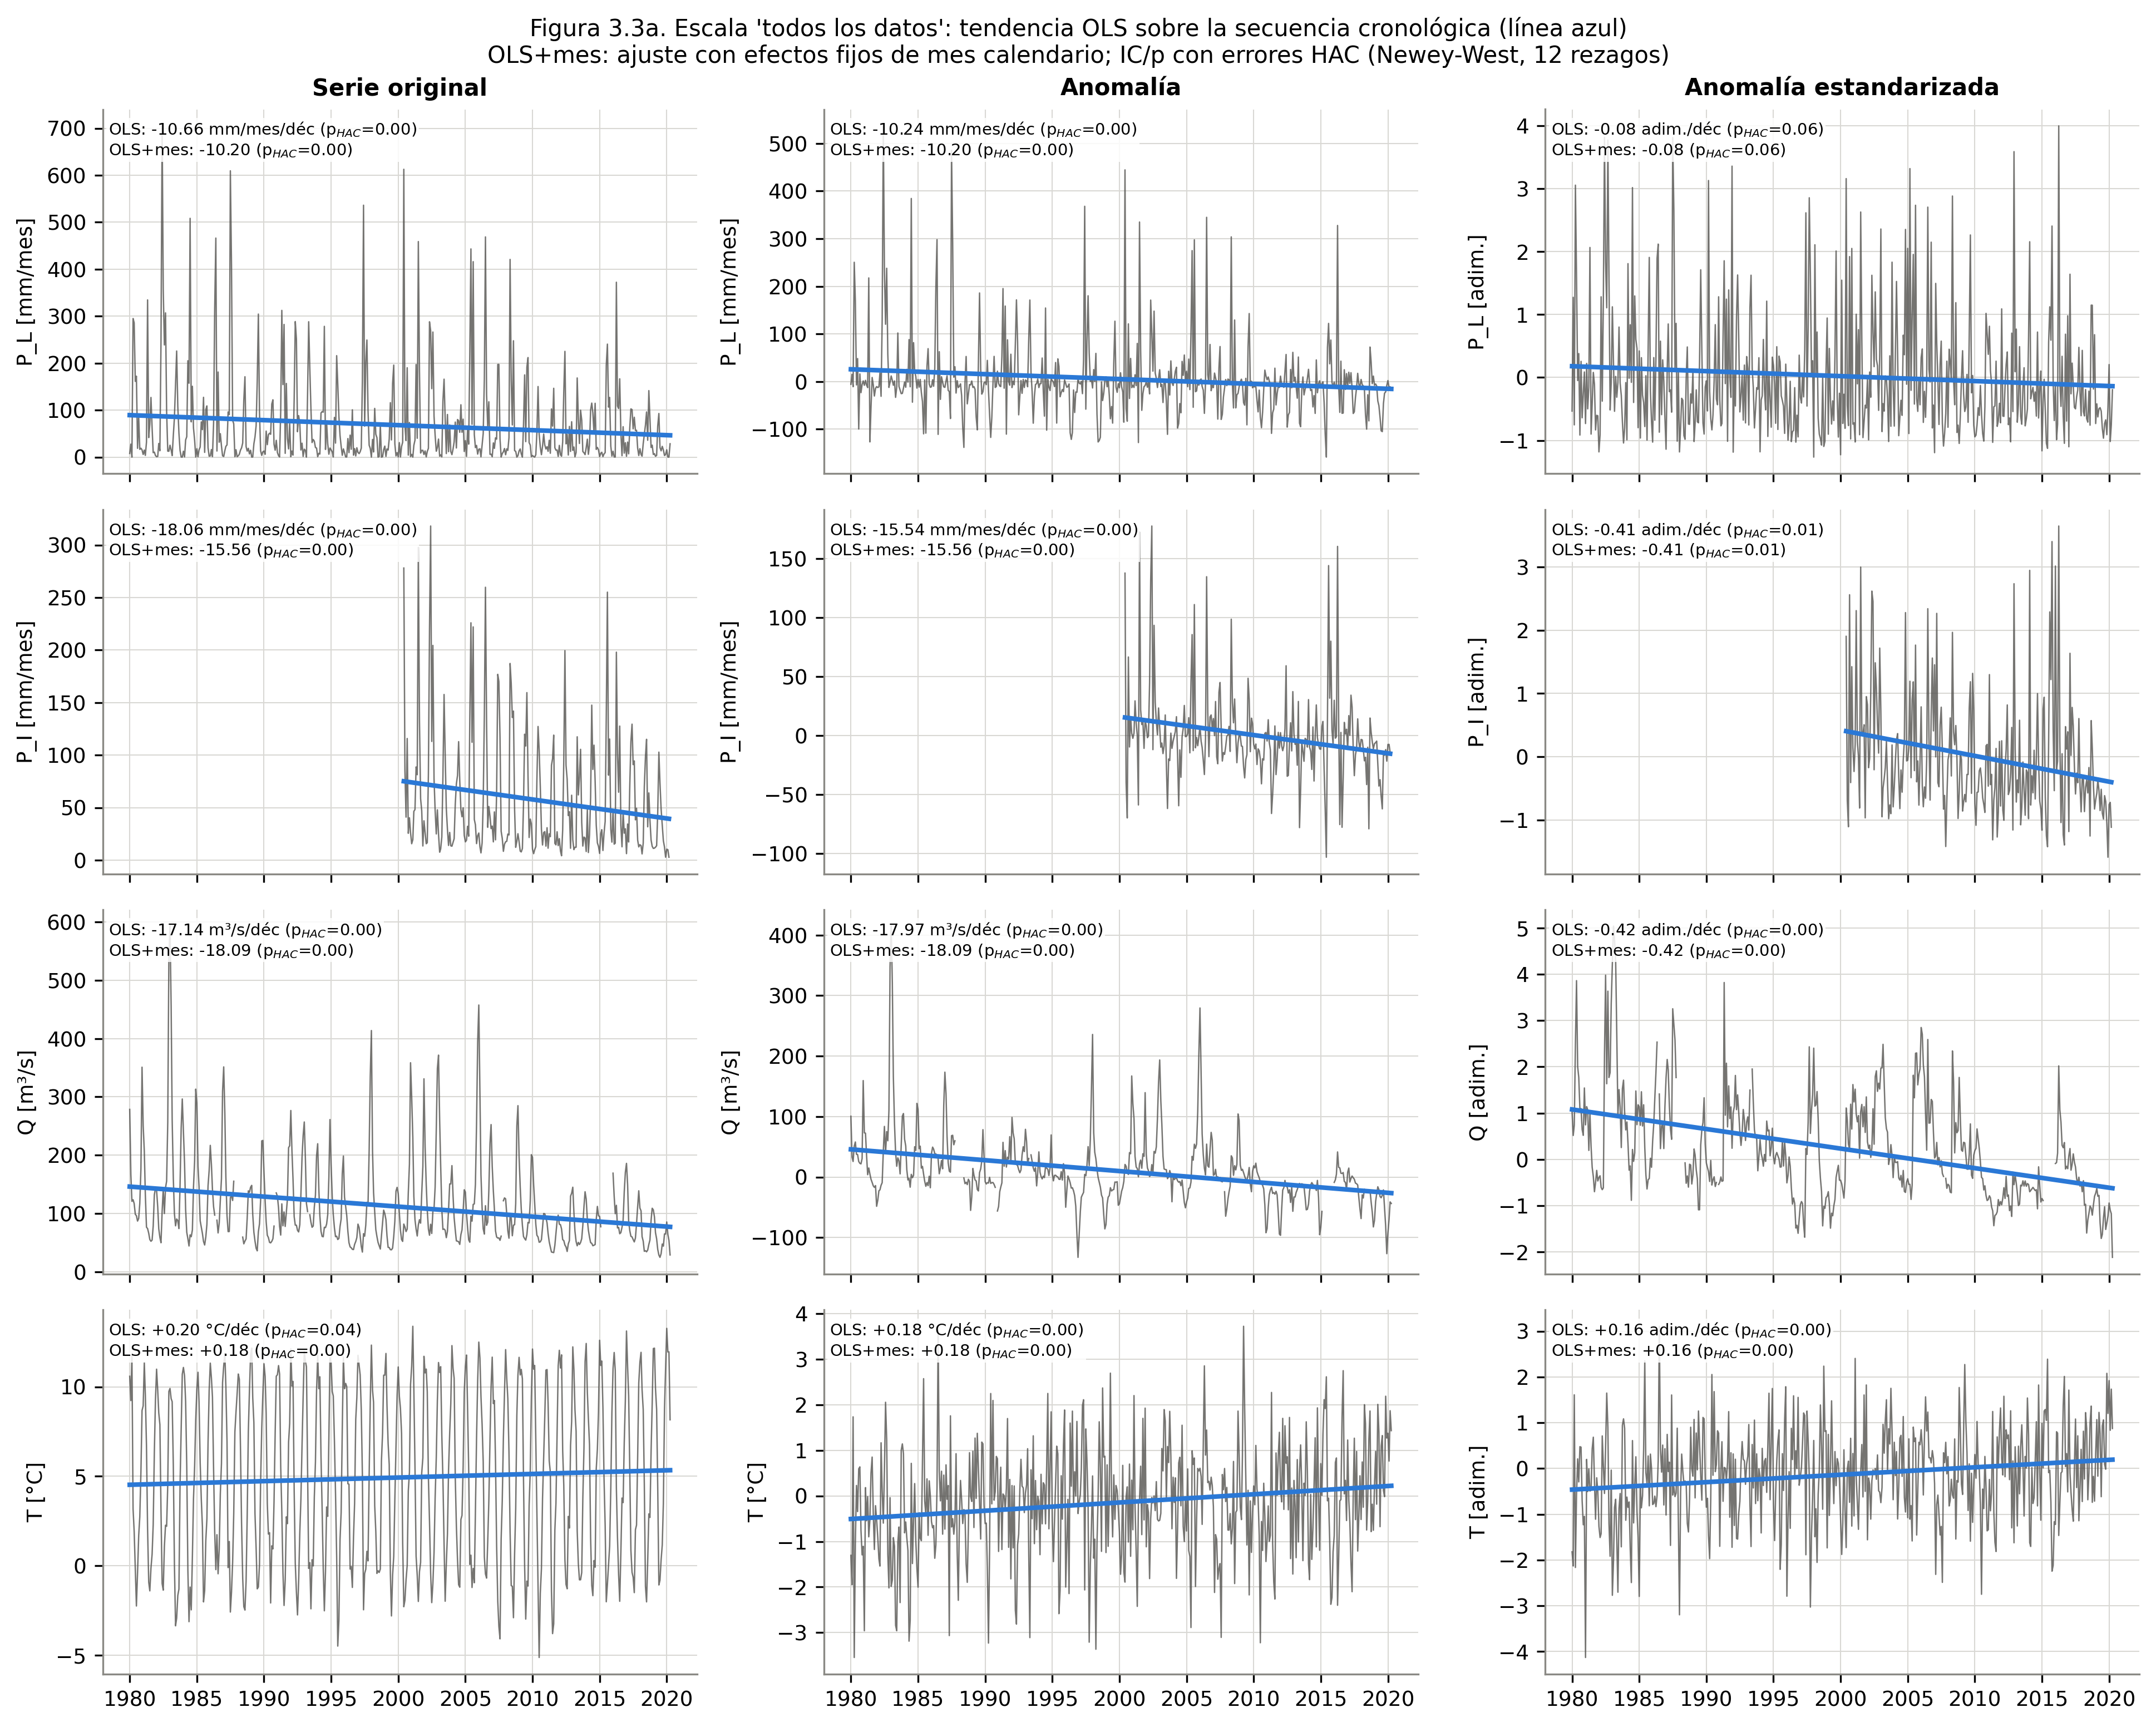
\includegraphics[width=0.95\textwidth]{figura_3_3a_todos_los_datos.png}
\caption{Escala ``todos los datos'': tendencia OLS sobre la secuencia cronológica; en el recuadro, el ajuste con efectos de mes calendario. IC y valores $p$ con errores HAC. Script \archivo{10_p3_3_escalas_temporales.py}.}
\label{fig:global}
\end{figure}

\subsubsection{Métodos y comparación (3.4)}

\begin{table}[H]
\centering\footnotesize
\caption{Comparación de métodos a escala global (\archivo{figuras/tabla_3_5_comparacion_metodos.csv} y \archivo{tabla_3_5_fdr_global.csv}). Pendientes por década, IC del 95\,\%; en precipitación, mm/mes por década del acumulado mensual. $q$: valor ajustado por FDR en la familia global de 12 pruebas.}
\label{tab:metodos}
\resizebox{\textwidth}{!}{\begin{tabular}{llrlrr}
\toprule
Variable (periodo, $n$) & Método & Pendiente & IC 95\,\% & $p$ & $q_{\mathrm{FDR}}$ \\
\midrule
$\PL$ (1980--2020, 484) & OLS sobre $a$ (HAC) & $-10.2$ & [$-17.3$, $-3.2$] & 0.004 & 0.007 \\
 & Theil--Sen sobre $a$ (MK Hamed--Rao) & $-3.3$ & [$-6.8$, $-0.3$] & 0.026 & 0.028 \\
 & Sen estacional sobre $X$ (bootstrap) & $-1.1$ & [$-2.9$, 0.1] & 0.081 & 0.081 \\
 & OLS sobre $z$ [$z$/década] & $-0.08$ & [$-0.16$, 0.00] & 0.062 & -- \\
\midrule
$\PI$ (2000--2020, 238) & OLS sobre $a$ (HAC) & $-15.5$ & [$-26.0$, $-5.1$] & 0.004 & 0.007 \\
 & Theil--Sen sobre $a$ (MK Hamed--Rao) & $-9.3$ & [$-15.9$, $-3.2$] & 0.002 & 0.006 \\
 & Sen estacional sobre $X$ (bootstrap) & $-8.1$ & [$-12.6$, $-4.7$] & 0.013 & 0.016 \\
\midrule
$\Qm$ (1980--2020, 463) & OLS sobre $a$ (HAC) [m$^3$/s/década] & $-18.0$ & [$-26.6$, $-9.3$] & $<0.001$ & 0.001 \\
 & Theil--Sen sobre $a$ (MK Hamed--Rao) & $-14.8$ & [$-22.3$, $-7.6$] & $<0.001$ & 0.001 \\
 & Sen estacional sobre $X$ (bootstrap) & $-12.2$ & [$-14.7$, $-9.7$] & 0.005 & 0.007 \\
 & OLS sobre $z$ [$z$/década] & $-0.42$ & [$-0.61$, $-0.23$] & $<0.001$ & -- \\
\midrule
$T$ CR2MET (1980--2020, 484) & OLS sobre $a$ (HAC) [$^\circ$C/década] & $+0.18$ & [0.07, 0.29] & 0.001 & 0.004 \\
 & Theil--Sen sobre $a$ (MK Hamed--Rao) & $+0.18$ & [0.07, 0.29] & 0.002 & 0.006 \\
 & Sen estacional sobre $X$ (bootstrap) & $+0.18$ & [0.08, 0.27] & 0.006 & 0.008 \\
\midrule
$T$ CR2MET (2000--2020, 238) & OLS sobre $a$ (HAC) [$^\circ$C/década] & $+0.25$ & [$-0.05$, 0.55] & 0.10 & -- \\
$T_{\mathrm{E5L}}$ (2000--2020, 238) & OLS sobre $a$ (HAC) [$^\circ$C/década] & $+0.28$ & [$-0.17$, 0.73] & 0.22 & -- \\
 & Theil--Sen sobre $a$ (MK Hamed--Rao) & $+0.29$ & [$-0.15$, 0.72] & 0.19 & -- \\
\bottomrule
\end{tabular}}
\end{table}

\begin{figure}[H]
\centering
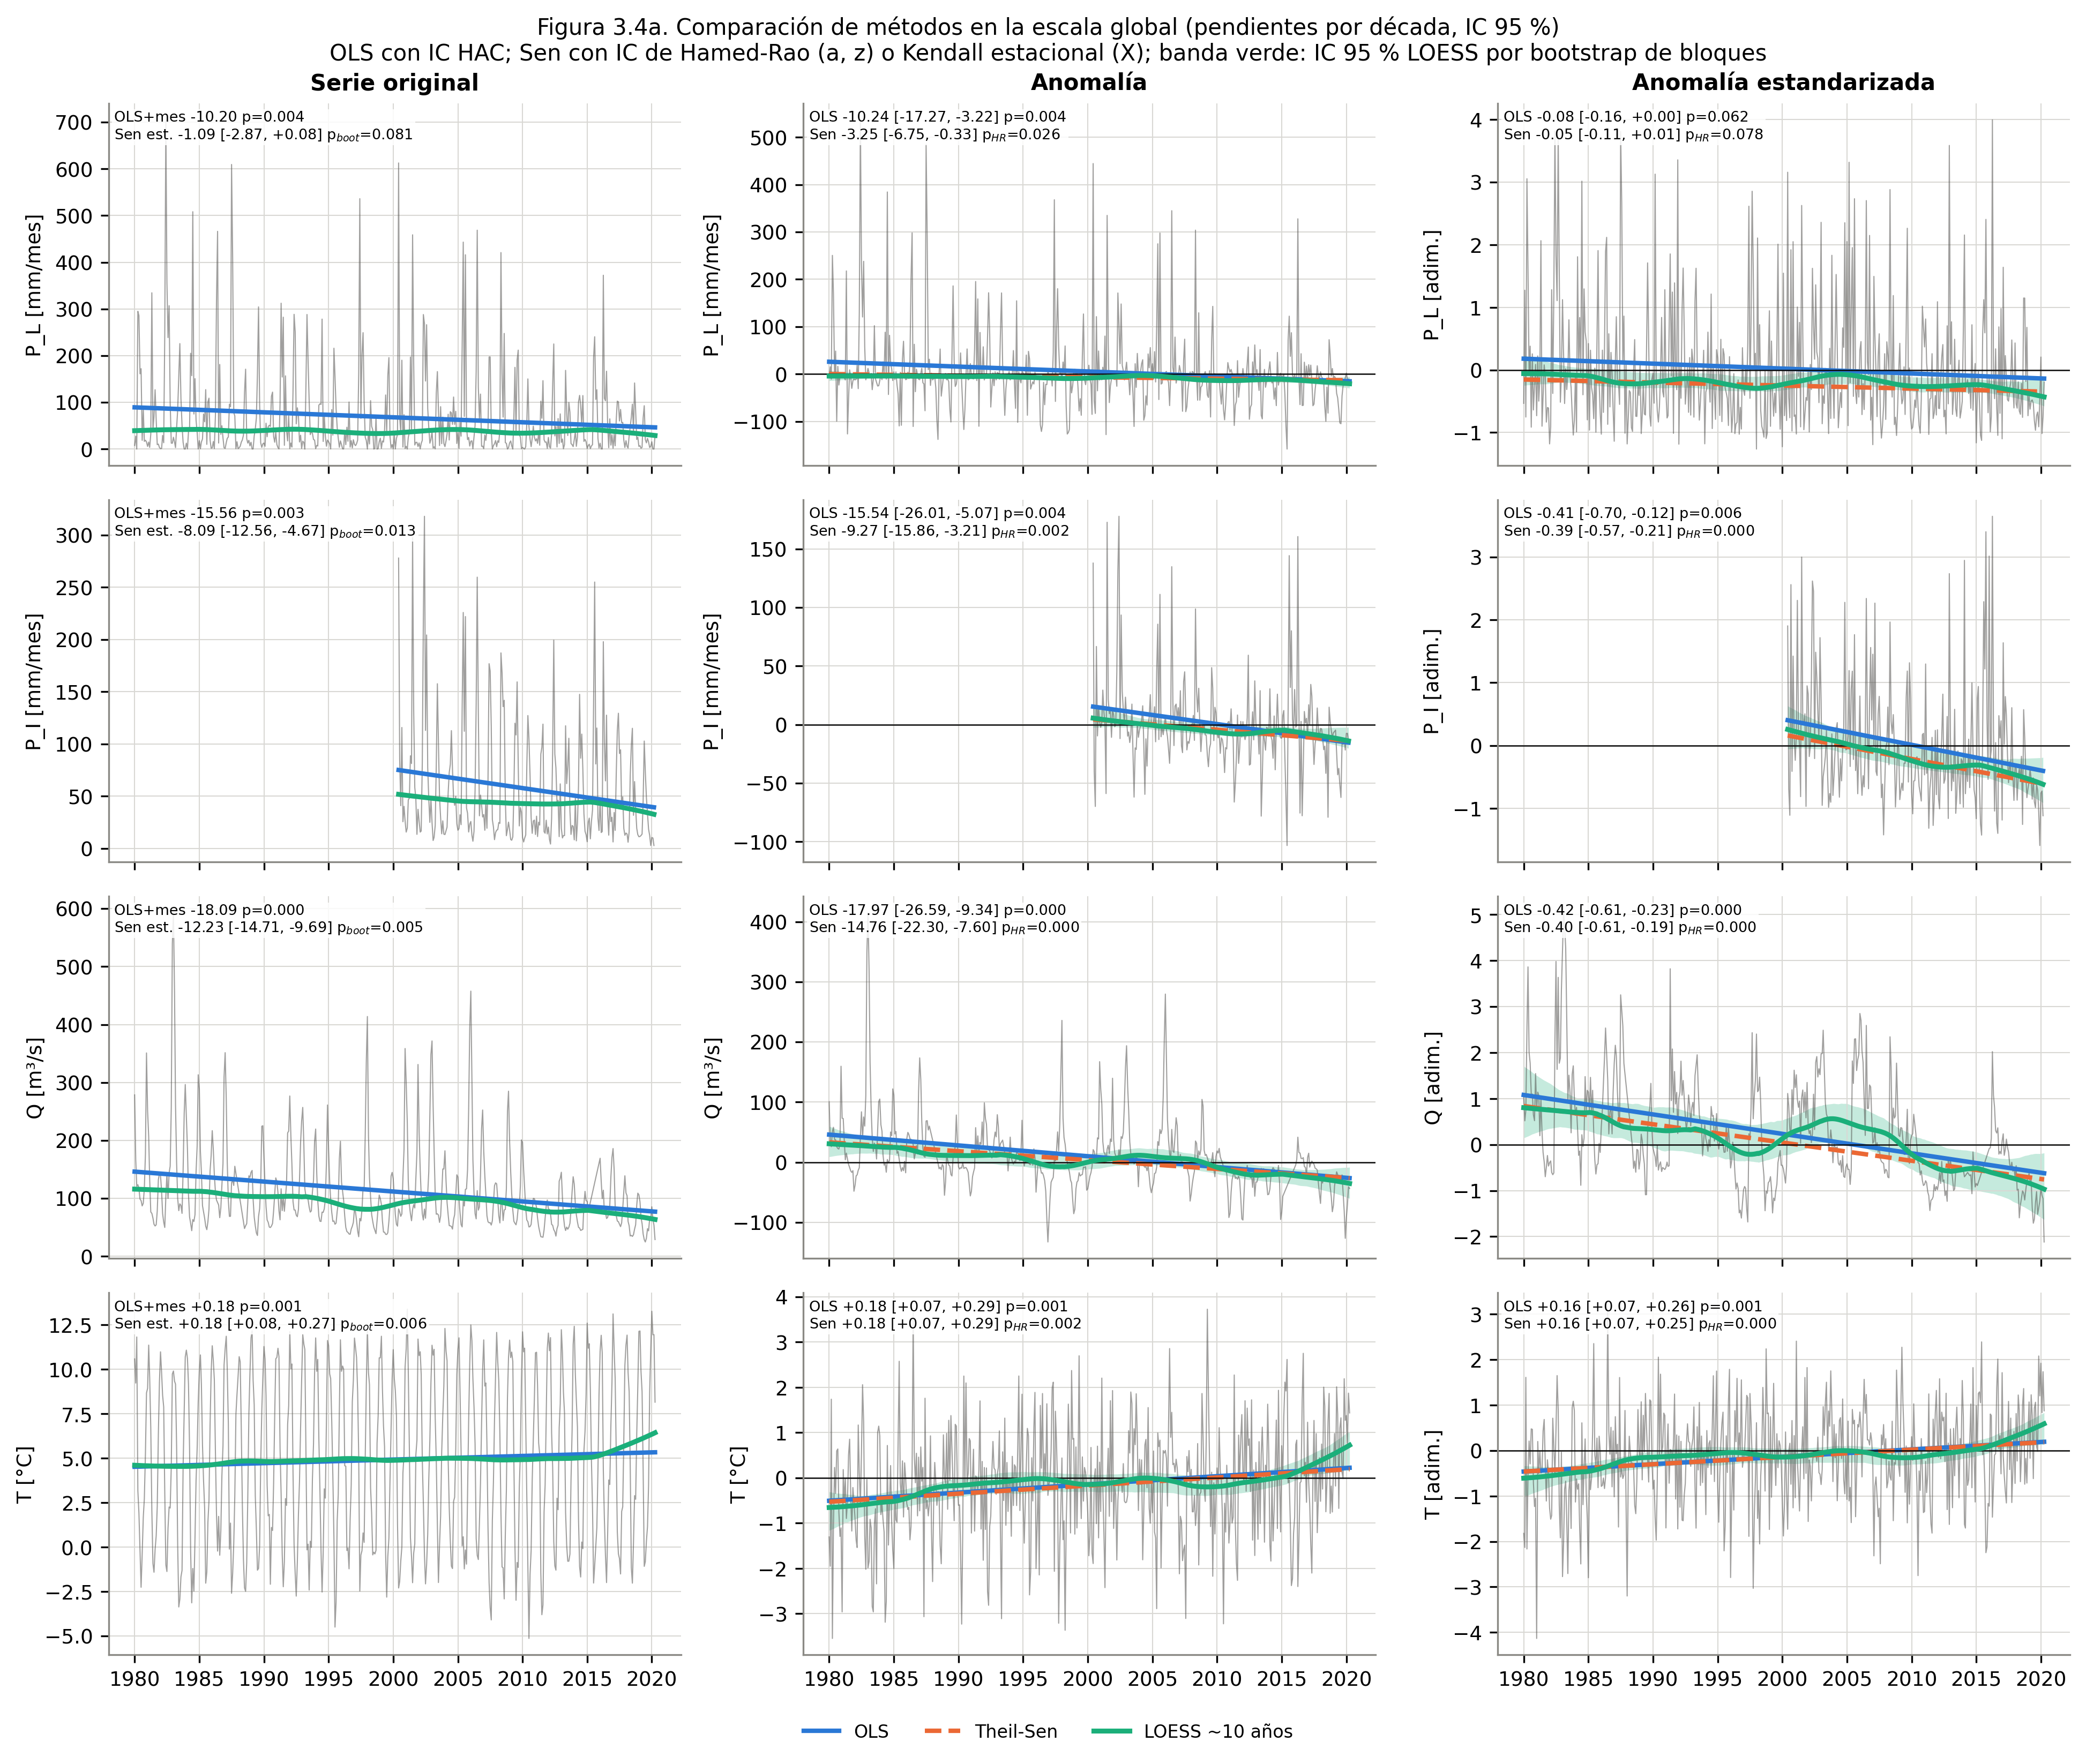
\includegraphics[width=0.95\textwidth]{figura_3_4a_metodos_global.png}
\caption{OLS (azul), Theil--Sen (naranja, discontinua) y LOESS de unos 10 años (verde, con IC del 95\,\% por bootstrap de bloques) en las tres representaciones. Script \archivo{11_p3_4_metodos_tendencia.py}.}
\label{fig:metodos}
\end{figure}

Los residuos de la OLS están autocorrelacionados (Figura~\ref{fig:resid}). En las anomalías del caudal la autocorrelación de rezago 1 es 0.80 y Ljung--Box rechaza la independencia; en $\PL$ es 0.14 y Breusch--Pagan indica heterocedasticidad ($p=0.02$). Por eso la inferencia se apoya en errores HAC y en las variantes corregidas de Mann--Kendall, no en los errores estándar usuales. El factor de Hamed--Rao para las anomalías del caudal es 6.4: la persistencia multiplica por más de seis la varianza del estadístico, y aun así la tendencia es significativa. Las tres familias de métodos difieren por diseño. OLS estima un cambio medio y es sensible a extremos; Theil--Sen estima una pendiente mediana robusta; el Sen estacional compara solo meses iguales y diluye una señal concentrada en pocos meses. LOESS describe la forma sin suponer linealidad.

\subsubsection{Incertidumbre, robustez y presentación (3.5)}

\begin{figure}[H]
\centering
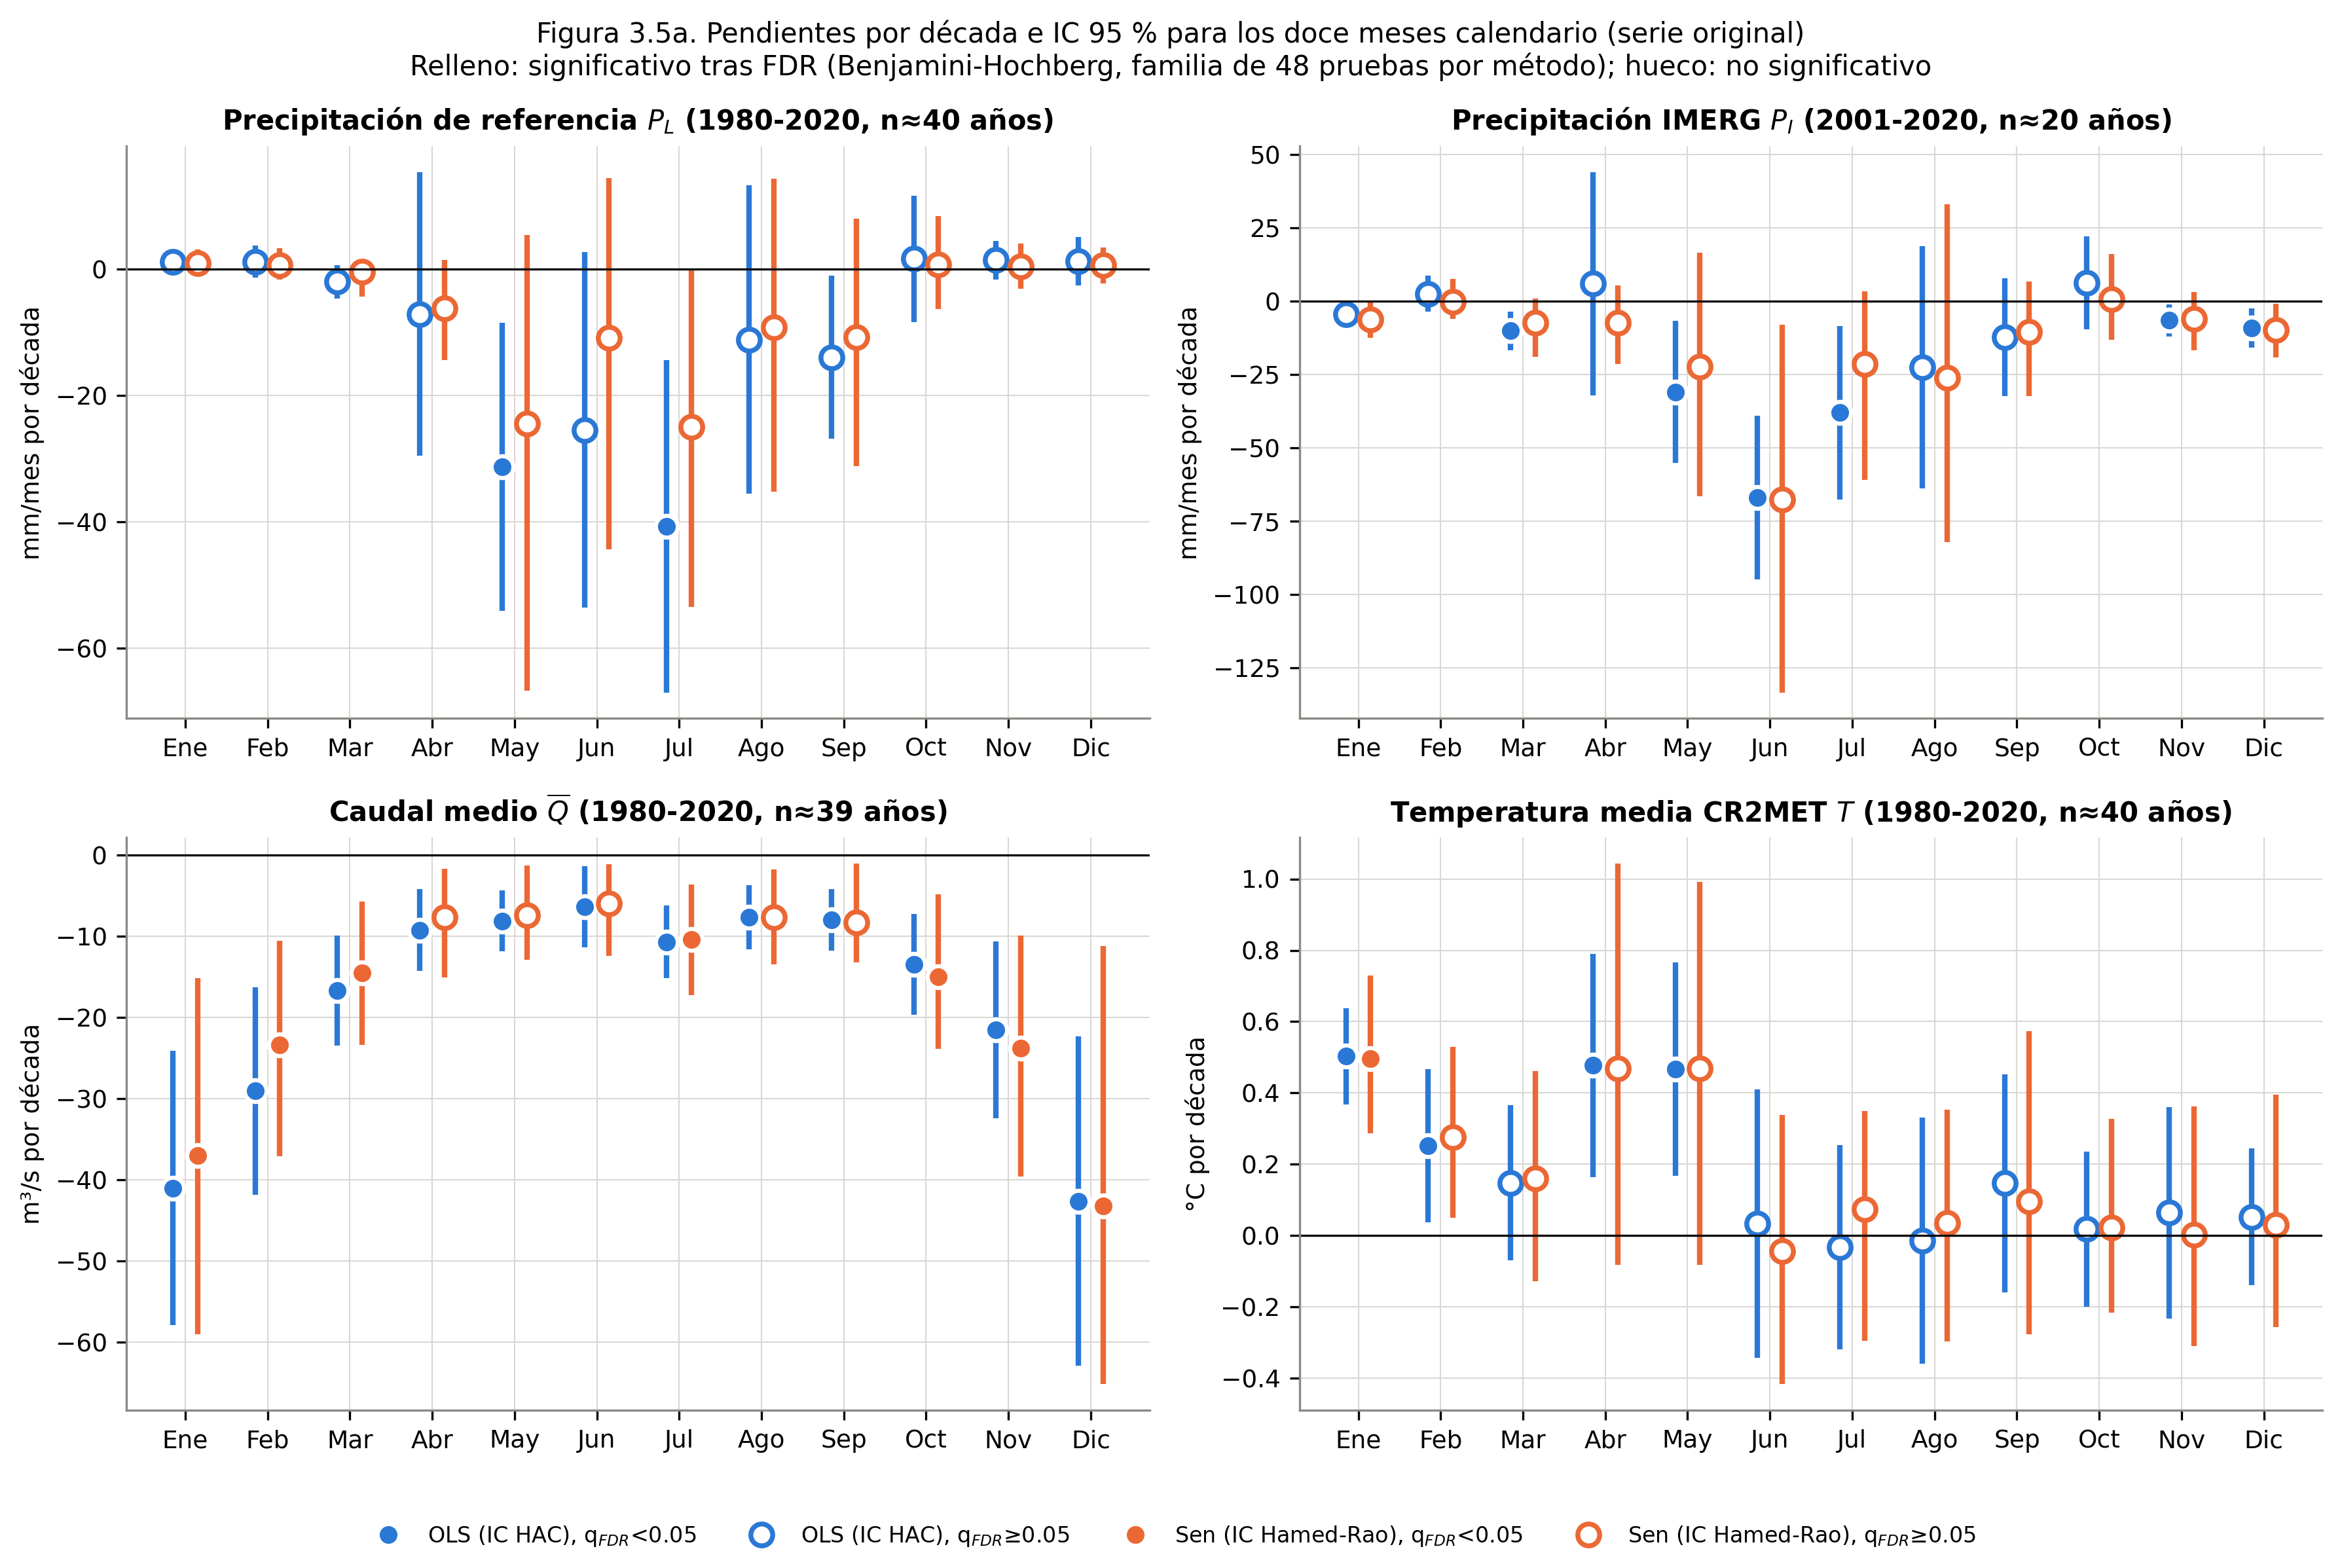
\includegraphics[width=0.95\textwidth]{figura_3_5a_pendientes_mensuales_ic.png}
\caption{Pendientes por década e IC del 95\,\% de los doce meses: OLS con IC HAC y Theil--Sen con IC de Hamed--Rao. Marcador relleno: significativo tras FDR en la familia de 48 pruebas de cada método. Script \archivo{12_p3_5_incertidumbre_robustez.py}.}
\label{fig:pendmes}
\end{figure}

\begin{table}[H]
\centering\footnotesize\setlength{\tabcolsep}{3pt}
\caption{Pendiente OLS por mes calendario (por década; $\PL$, $\Qm$ y $T$ CR2MET en 1980--2020, $\PI$ en 2000--2020) y significancia tras FDR (\archivo{figuras/tabla_3_5_fdr_mensual.csv}). $^{*}$: $q<0.05$ con OLS-HAC; $^{\dagger}$: además $q<0.05$ con Mann--Kendall de Hamed--Rao.}
\label{tab:pendmes}
\begin{tabular}{lrrrrrrrrrrrr}
\toprule
 & Ene & Feb & Mar & Abr & May & Jun & Jul & Ago & Sep & Oct & Nov & Dic \\
\midrule
$\PL$ [mm/mes] & 1.2 & 1.2 & $-2.0$ & $-7.1$ & $-31.3^{*}$ & $-25.4$ & $-40.7^{*}$ & $-11.2$ & $-13.9$ & 1.6 & 1.4 & 1.2 \\
$\PI$ [mm/mes] & $-4.4$ & 2.6 & $-10.1^{*}$ & 6.0 & $-31.0^{*}$ & $-67.0^{*}$ & $-38.0^{*}$ & $-22.5$ & $-12.3$ & 6.3 & $-6.5^{*}$ & $-9.1^{*}$ \\
$\Qm$ [m$^3$/s] & $-41.0^{\dagger}$ & $-29.1^{\dagger}$ & $-16.7^{\dagger}$ & $-9.2^{*}$ & $-8.1^{*}$ & $-6.4^{*}$ & $-10.7^{\dagger}$ & $-7.7^{*}$ & $-8.0^{*}$ & $-13.5^{\dagger}$ & $-21.5^{\dagger}$ & $-42.6^{\dagger}$ \\
$T$ [$^\circ$C] & $0.50^{\dagger}$ & $0.25^{*}$ & 0.15 & $0.48^{*}$ & $0.47^{*}$ & 0.03 & $-0.03$ & $-0.01$ & 0.15 & 0.02 & 0.06 & 0.05 \\
\bottomrule
\end{tabular}
\end{table}

\begin{figure}[H]
\centering
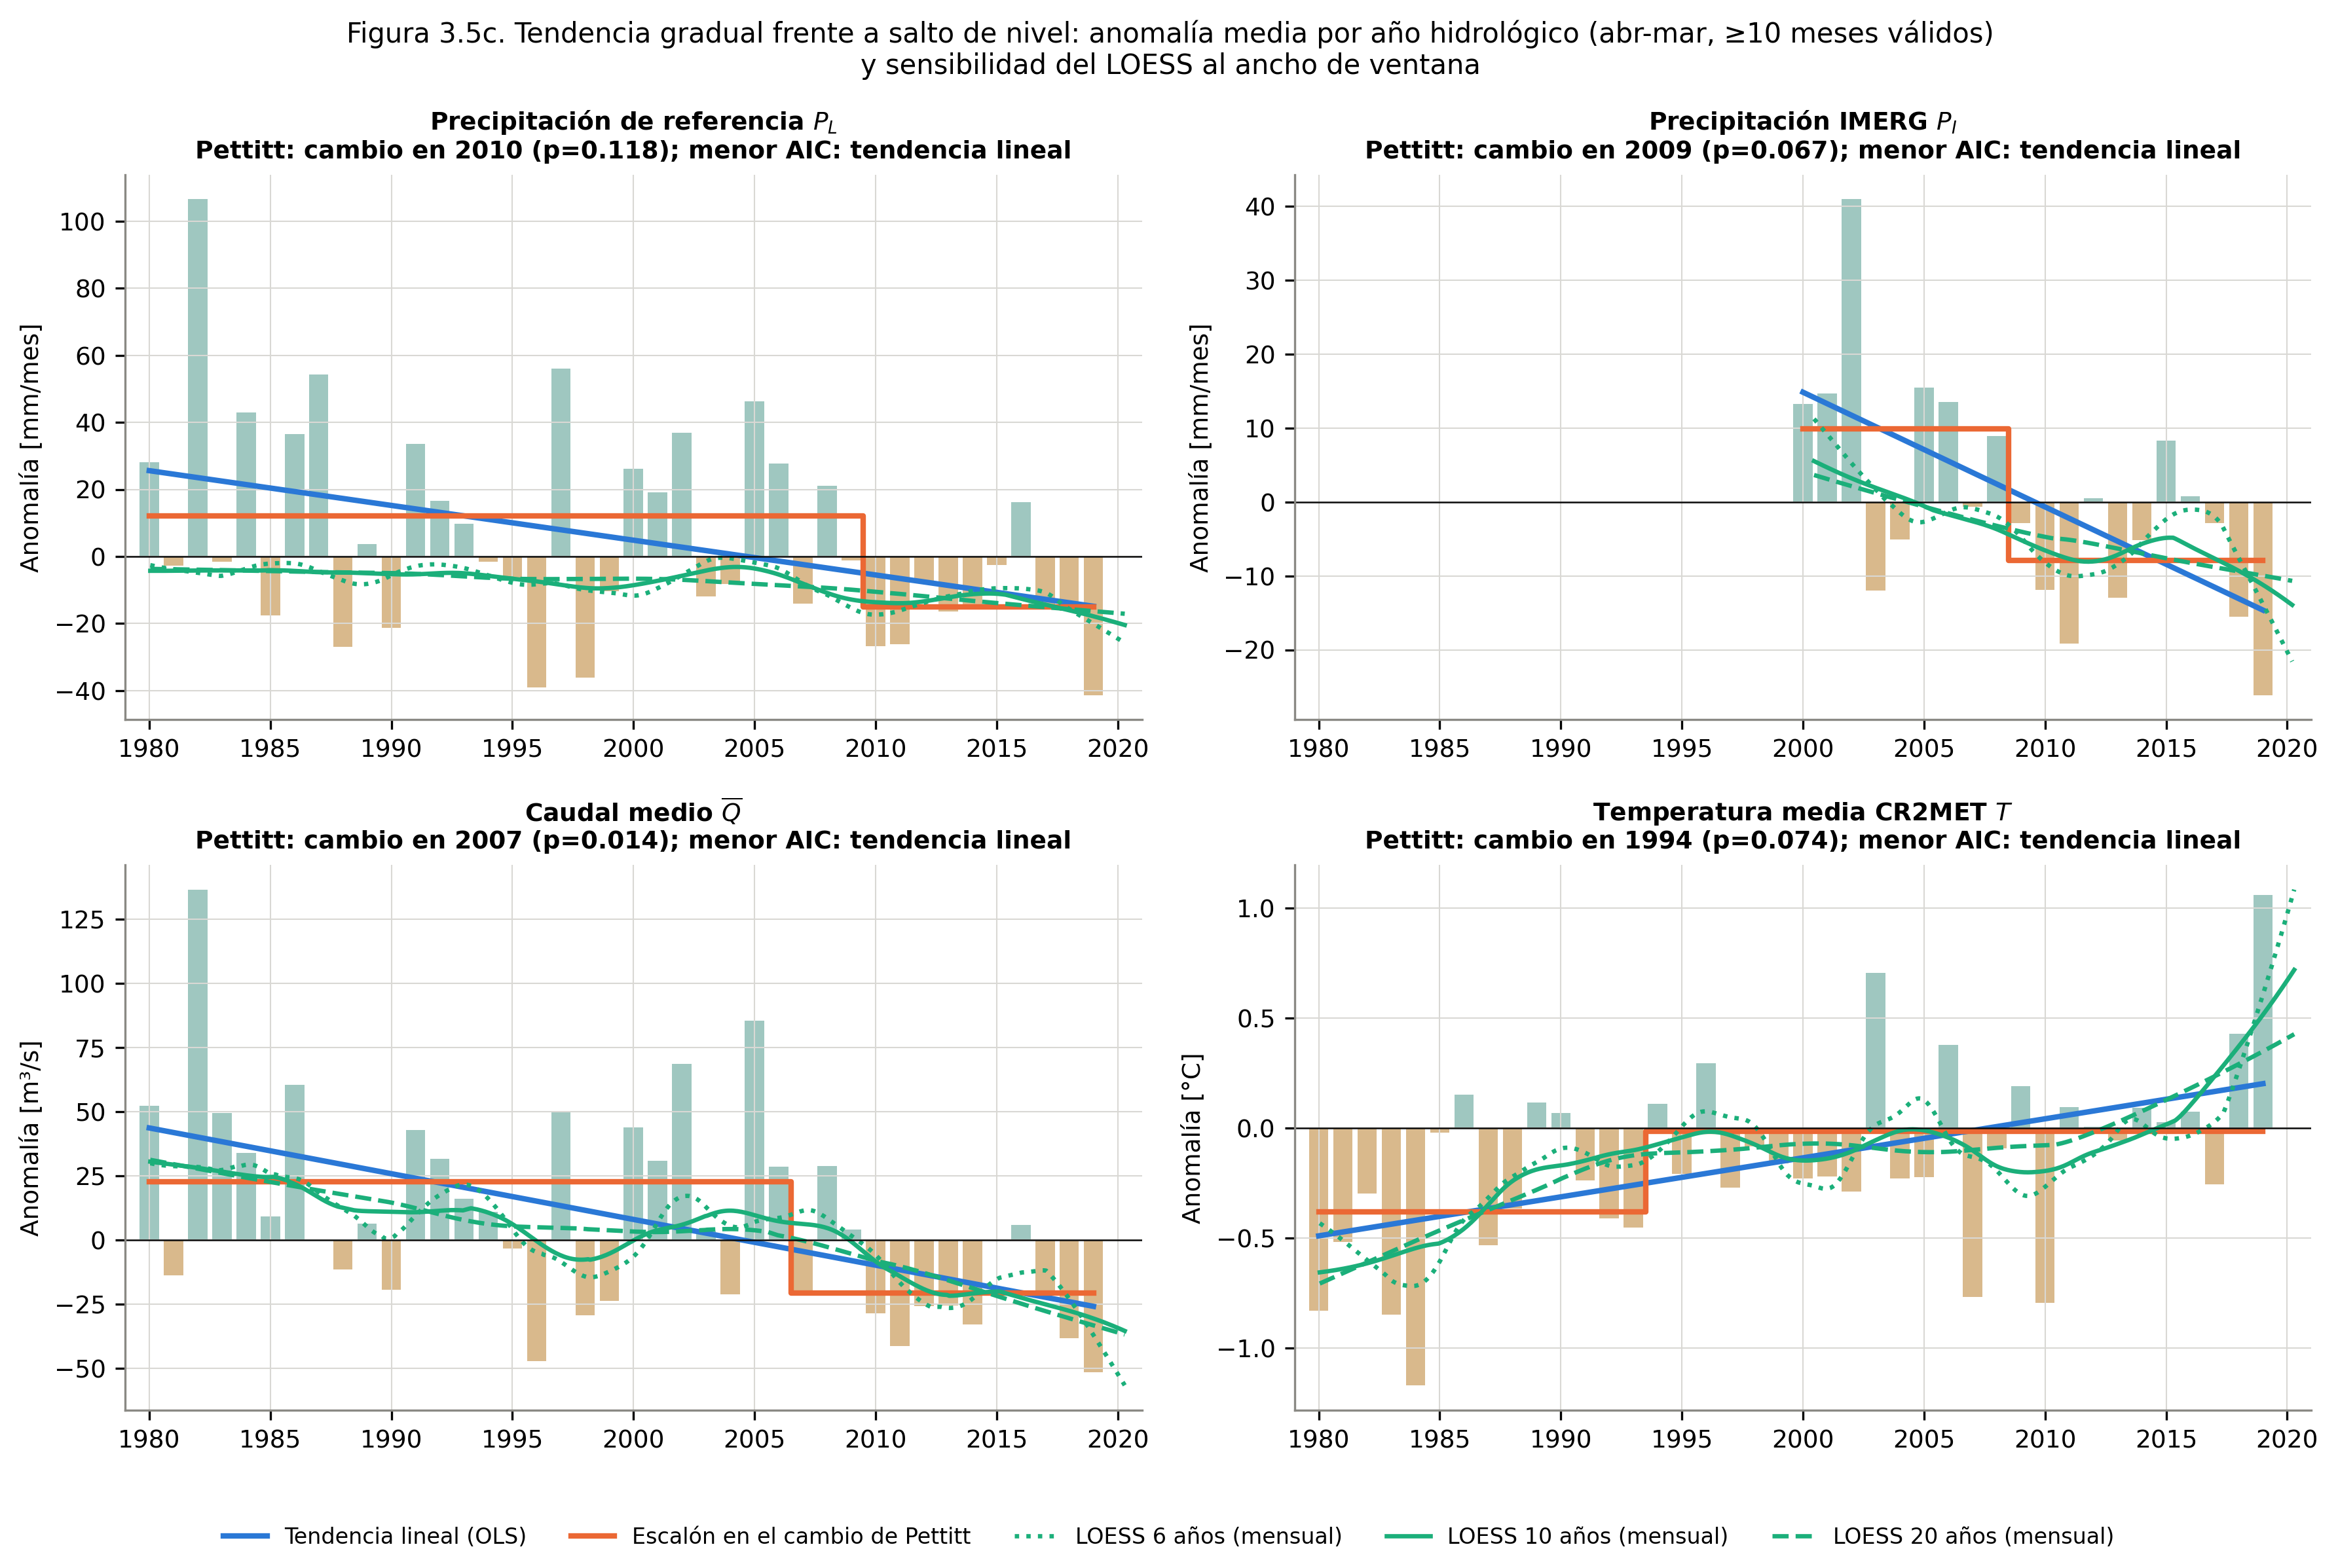
\includegraphics[width=0.9\textwidth]{figura_3_5c_salto_vs_tendencia.png}
\caption{Anomalía media por año hidrológico con tendencia lineal, escalón en el año de cambio de Pettitt y LOESS de 6, 10 y 20 años. El LOESS robusto queda por debajo de la media en los años húmedos porque resta peso a las anomalías extremas de una variable asimétrica.}
\label{fig:salto}
\end{figure}

\paragraph{Resultados estadísticos.}
\begin{enumerate}
\item \textbf{Caudal}: disminuye en los doce meses, con todos los métodos y representaciones. A escala global el descenso es de 12 a 18~m$^3$/s por década, entre 11 y 20\,\% de la media mensual por década. Mes a mes, los mayores descensos absolutos ocurren en diciembre y enero ($-43$ y $-41$~m$^3$/s por década), en pleno deshielo. Tras el FDR, los 12 meses son significativos con OLS-HAC y 7 con Mann--Kendall corregido. Sin los tres años hidrológicos más húmedos la pendiente anual baja de $-17.8$ a $-13.8$~m$^3$/s por década, sin cambiar de signo ni perder significancia. El mayo de 1993 incompleto ya no entra en el análisis; la pendiente de mayo es de $-8.1$~m$^3$/s por década y significativa.
\item \textbf{Precipitación de referencia}: el descenso se concentra en el invierno (mayo $-31$ y julio $-41$~mm/mes por década, un 24--28\,\% de la media mensual). En verano las pendientes son nulas o ligeramente positivas. Tras el FDR solo mayo y julio son significativos con OLS-HAC, y ningún mes con Mann--Kendall. Globalmente, OLS y Sen sobre $a$ son significativos, pero el Sen estacional ($-1.1$, $p=0.08$) y $z$ ($p=0.06$) no lo son, porque dan el mismo peso a los meses secos, que no cambian.
\item \textbf{IMERG}: disminuye de 8 a 16~mm/mes por década en su registro de 20 años, con mayor caída en mayo--julio. Coincide con $\PL$ en el signo, pero no en la magnitud: en el periodo común, $\PL$ cae $-24.3$~mm/mes por década y $\PI$ $-15.5$.
\item \textbf{Temperatura}: la temperatura de la base (CR2MET) aumenta $+0.18$~$^\circ$C por década en 1980--2020 (IC [0.07, 0.29]), con los tres métodos y tras el FDR. Un calentamiento gradual explica mejor la serie que un escalón ($\Delta\mathrm{AIC}=-3.3$ a favor de la tendencia). Mes a mes se concentra en verano y otoño (enero $+0.50$, abril $+0.48$ y mayo $+0.47$~$^\circ$C por década) y es nulo de junio a agosto. En la ventana 2000--2020, CR2MET da $+0.25$ ($p=0.10$) y ERA5-Land $+0.28$ ($p=0.22$): las dos fuentes coinciden, pero 20 años no bastan para detectar la tendencia (\archivo{figuras/tabla_3_1_tendencia_temperatura_cr2met.csv}).
\item \textbf{Forma del cambio}: no es lineal ni homogénea. Hasta 2009 las pendientes de $\PL$ ($-6.4$, $p=0.15$) y $\Qm$ ($-9.3$, $p=0.16$) no son significativas. El LOESS muestra un aumento en 1998--2004 y caídas fuertes en 2004--2013 y 2015--2020. Pettitt sitúa un cambio en 2007 para el caudal ($p=0.014$) y en 2010 para la lluvia ($p=0.12$). La tendencia lineal y el escalón tienen un AIC casi igual ($\Delta\mathrm{AIC}\approx0.2$), de modo que \emph{los datos no permiten distinguir una tendencia gradual de un salto de nivel}. El signo negativo domina el 86\,\% de las ventanas de al menos 15 años en $\PL$ y el 84\,\% en $\Qm$. Las ventanas que empiezan después de 1987 y terminan entre 2002 y 2010 tienen pendiente positiva.
\end{enumerate}
El estudio recomendado por la guía encontró en Australia que la mayoría de los cambios de nivel en caudal se produjeron antes del inicio formal de la ``sequía del milenio'' y combinó MK con corrección de varianza, bootstrap por bloques y Pettitt \citep{Amirthanathan2023}. Nuestro cambio de 2007 en el caudal, anterior al inicio de la megasequía en 2010, muestra una cronología análoga y se obtuvo con los mismos métodos. No aplicamos su variante para persistencia de largo plazo (MK4), que queda como mejora pendiente.

\subsubsection{¿A qué podrían deberse los cambios? (3.6)}
\label{sec:p36}

\paragraph{Contraste entre precipitación, caudal y temperatura.} Las variables no cambian en los mismos meses, pero sí en el mismo periodo, y de forma coherente con el régimen nival. La lluvia baja en los meses de acumulación (mayo--septiembre) y el caudal baja en todos los meses, sobre todo en el deshielo de diciembre a febrero (Figura~\ref{fig:pendmes}). Es la transferencia estacional que cabe esperar si un déficit de nieve invernal reduce el deshielo de primavera y verano \citep{Masiokas2006}. En el tiempo, $\PL$ y $\Qm$ comparten el punto de cambio (2007--2010) y las fases del LOESS, al inicio de la megasequía de Chile central \citep{Garreaud2017,Garreaud2020}.

\paragraph{¿Responde el caudal de manera consistente con la lluvia?} En magnitud, sí (\archivo{scripts/25_p3_6_balance_anual.py}; \archivo{figuras/tabla_3_6_balance_resumen.csv}). En los años hidrológicos con los doce meses válidos, la precipitación media bajó de 919~mm (1980--2009, 24 años) a 555~mm (2010--2019, 8 años), un $-40$\,\%, y la escorrentía bajó de 821 a 479~mm, un $-42$\,\%. La elasticidad aparente es de 1.05, del orden de la de 0.80 que CAMELS-CL estima para 1979--2010. El cociente $R/P$ pasa de 0.95 a 0.91 sin tendencia significativa (Sen de $-0.009$ por década, $p=0.66$). Una regresión anual $R=1.0+0.69P_t+0.19P_{t-1}$ ($R^2=0.92$, 31 años; el término del año previo es significativo, $p<0.001$) deja un residuo medio de $+10$~mm/año antes de 2010 y de $-30$~mm/año después: tras descontar la lluvia del año y la del anterior queda un déficit adicional pequeño. Ese déficit es compatible con el agotamiento progresivo de almacenamientos (nieve remanente y agua subterránea) descrito para cuencas chilenas de memoria larga durante sequías plurianuales \citep{AlvarezGarreton2021}, pero con ocho años posteriores a 2010 no es una prueba.

\paragraph{Evapotranspiración, nieve y deshielo.} Un calentamiento elevaría la línea de nieves, adelantaría el deshielo y aumentaría la sublimación y la evapotranspiración, lo que podría explicar el déficit residual. La temperatura de la base aumenta 0.18~$^\circ$C por década en 40 años, de magnitud comparable a las tendencias andinas documentadas \citep{Falvey2009}, y ERA5-Land concuerda en el periodo común. Pero la distribución estacional del calentamiento importa: es casi nulo de junio a agosto, de modo que la isoterma invernal apenas sube (+18~m por década, no significativo; Sección~\ref{sec:isoterma}) y no hay evidencia de que la acumulación de nieve se haya reducido por temperatura. El calentamiento de abril--mayo y de verano sí puede hacer más líquidas las primeras tormentas del otoño y aumentar la sublimación y la evapotranspiración del deshielo. Es un candidato plausible para el déficit residual después de 2010, pero no la causa principal de la caída del caudal, que sigue a la lluvia.

\paragraph{Rezagos y fuentes de lluvia.} La persistencia del caudal (autocorrelación de 0.80 en las anomalías) hace que un déficit de lluvia afecte varios meses de caudal, y por eso la tendencia del caudal tiene mayor evidencia estadística que la de la lluvia. Entre fuentes, la diferencia $\PI-\PL$ por año hidrológico aumenta $+106$~mm/año por década (Sen; $p=0.06$ con Mann--Kendall corregido y 0.03 con OLS-HAC), y el cociente anual $\PI/\PL$ varía entre 0.67 y 1.44 sin un patrón estable: las dos fuentes coinciden en el signo, pero no en la magnitud.

\paragraph{Contexto de la cuenca.} Aguas arriba de El Manzano existe el embalse El Yeso, que regula el río Yeso para el abastecimiento de agua potable de Santiago, y CAMELS-CL registra derechos consuntivos superficiales equivalentes al 20\,\% del caudal medio. El embalse es anterior al periodo de estudio, por lo que su existencia no genera por sí sola una tendencia; un aumento de las extracciones sí podría acentuarla. También hay centrales hidroeléctricas de pasada, que desvían y restituyen agua; el proyecto Alto Maipo entró en operación después del periodo analizado. La cuenca es de alta montaña, casi sin urbanización (0.1\,\%) ni bosques (0.2\,\%), por lo que es improbable que un cambio de cobertura explique una caída del 40\,\% del caudal. No hay registro documentado de un cambio de la estación que explique el vacío de 2015. El argumento más fuerte contra una causa antrópica local dominante es que el caudal baja en proporción a la lluvia y en todos los meses, no solo en los de operación de un embalse. Sin los registros de extracción y de operación de El Yeso no podemos reconstruir el caudal natural para confirmarlo.

\paragraph{Clima, variabilidad y observación.} El registro empieza en una década húmeda (1980--1987, con los El Niño de 1982 y 1987) y termina en la megasequía (con 2019 como año más seco), lo que maximiza la pendiente. Sin los tres años más húmedos (1982, 1987 y 1997), la tendencia anual de $\PL$ baja de $-10.4$ a $-5.9$~mm/mes por década, y si el registro se corta en 2009 deja de ser significativa. Una fase de variabilidad interdecadal del Pacífico puede producir una tendencia aparente en 40 años: la lluvia invernal de Chile central se asocia con ENSO \citep{Montecinos2003}, y la megasequía se ha atribuido en buena parte a variabilidad natural, con una fracción antropogénica \citep{Boisier2016,Garreaud2020}. Nuestros datos no separan esos componentes. En cuanto a la observación: (i) CR2MET combina estaciones y reanálisis \citep{AlvarezGarreton2018}, y cambios en la red de estaciones o en el forzante podrían alterar su tendencia; (ii) IMERG une la era TRMM (hasta 2014) con la era GPM, lo que podría introducir inhomogeneidades coherentes con la deriva de $\PI-\PL$ \citep{Huffman2020}; (iii) ERA5-Land hereda los cambios del sistema de observación de ERA5 \citep{MunozSabater2021}; (iv) el caudal es la variable observada más directamente, y su tendencia coincide en signo con dos productos de lluvia procesados de forma independiente, aunque comparten pluviómetros.

\begin{table}[H]
\centering\footnotesize
\caption{Hipótesis sobre los cambios detectados y grado de evidencia.}
\label{tab:hipotesis}
\begin{tabularx}{\textwidth}{>{\raggedright\arraybackslash}p{2.3cm}>{\raggedright\arraybackslash}X>{\raggedright\arraybackslash}X>{\raggedright\arraybackslash}X>{\raggedright\arraybackslash}p{2.4cm}}
\toprule
Hipótesis & Mecanismo & Evidencia favorable & Evidencia faltante o contradictoria & Datos necesarios \\
\midrule
H1. Déficit de lluvia invernal (megasequía) & Menos nieve acumulada, menor deshielo, menor caudal en todos los meses & Caída invernal de $\PL$ y $\PI$; caída de $\Qm$ en 12 meses; cambio común en 2007--2010; elasticidad de 1.05 \citep{Garreaud2017,Garreaud2020} & Sin tendencia significativa hasta 2009; la tendencia de $\PL$ no supera el FDR con Sen estacional & Equivalente en agua de nieve; pluviómetros de altura \\
H2. Memoria y agotamiento de almacenamientos & La sequía plurianual vacía la nieve remanente y los acuíferos & Residuo de $-30$~mm/año después de 2010; $P_{t-1}$ significativo en el balance anual; $r_1=0.80$; $R/P>1$ en años secos \citep{AlvarezGarreton2021} & $R/P$ sin tendencia significativa; pocos años después de 2010 & Niveles de pozos; caudal base \\
H3. Calentamiento & Más ETP y sublimación; deshielo temprano; más lluvia y menos nieve & $T$ CR2MET $+0.18$~$^\circ$C por década, robusta a métodos y FDR; concentrada en verano y otoño \citep{Falvey2009} & Nulo en pleno invierno; isoterma invernal sin tendencia significativa; ERA5-Land sin significancia en 20 años & Estaciones de altura; equivalente en agua de nieve; fechas de deshielo \\
H4. Regulación y extracciones & El Yeso y las captaciones reducen el caudal en El Manzano & Intervención documentada (IAI del 20\,\%, presa grande) & Caída proporcional a la lluvia y en todos los meses; embalse anterior al registro & Registros de extracción y operación; caudal natural \\
H5. Variabilidad decadal o artefacto del periodo & Inicio húmedo y final seco del registro & Gran sensibilidad a fechas y extremos \citep{Boisier2016} & Signo negativo en el 84--86\,\% de las ventanas & Registros más largos o reconstrucciones \\
H6. Inhomogeneidad de productos & Cambios en redes, TRMM/GPM o asimilación & Deriva $\PI-\PL$ ($p=0.06$) & El caudal observado confirma el signo & Pluviómetros DGA puntuales \\
\bottomrule
\end{tabularx}
\end{table}

\begin{purplebox}[title={Síntesis del punto 3}]
\begin{itemize}[leftmargin=*]
\item \textbf{¿Qué cambia, cuánto, en qué meses y periodo?} El caudal disminuye entre 12 y 18~m$^3$/s por década en 1980--2020, en los doce meses, con hasta 41~m$^3$/s por década en diciembre--enero. La precipitación de referencia disminuye unos 10~mm/mes por década (OLS), concentrada en mayo--julio. IMERG disminuye en 2000--2020. La temperatura de la base aumenta 0.18~$^\circ$C por década (1980--2020), sobre todo en verano y otoño; ERA5-Land concuerda, sin significancia en sus 20 años.
\item \textbf{¿Lineal, monotónico, no lineal o salto?} Es un descenso no lineal, compatible con una tendencia o con un cambio de nivel hacia 2007--2010; los datos no los distinguen.
\item \textbf{¿Qué tan robusto?} El caudal es robusto frente al método, la representación, los extremos, el criterio de completitud y la fecha inicial, pero no frente a la fecha final: sin 2010--2019 no hay tendencia significativa. La lluvia es robusta en el signo y sensible en la significancia.
\item \textbf{Explicación mejor sustentada}: H1 (déficit de lluvia invernal transmitido por la nieve), modulada por H2. H3 tiene evidencia térmica robusta, pero un calentamiento casi nulo en invierno no explica la caída de la acumulación de nieve; H4 es plausible sin evidencia propia suficiente; y H5 impide extrapolar las pendientes fuera de 1980--2020. Una tendencia estadística no permite atribuir el cambio a una causa, tampoco al cambio climático.
\item \textbf{Tipo de evidencia}: el caudal es una observación directa; $\PL$ es un producto grillado con estaciones; $\PI$ es satelital ajustado con pluviómetros; $T$ proviene de reanálisis o de un producto grillado. H1 a H6 son hipótesis de interpretación.
\end{itemize}
\end{purplebox}
\subsection{Punto 4. Análisis de frecuencias mediante Fourier}
\label{sec:p4}

\subsubsection{Series preparadas y documentación del cálculo (4.1)}

\begin{table}[H]
\centering\footnotesize
\caption{Documentación del cálculo espectral (\archivo{figuras/tabla_4_1_documentacion_espectral.csv}). $\Delta t=1$ mes; Nyquist de 0.5 ciclos/mes (periodo mínimo de 2 meses); periodo máximo representable de $N$ meses, con un solo ciclo observado.}
\label{tab:docesp}
\resizebox{\textwidth}{!}{\begin{tabular}{llrrrrl}
\toprule
Tramo & Variables & $N$ & Ciclos anuales & $\Delta f$ [ciclos/mes] & Meses rellenados & Tendencia retirada en AD \\
\midrule
1980-04 a 2020-03 & $\PL$, $\Qm$, $T$ & 480 & 40 & $2.08\times10^{-3}$ & 21 ($\Qm$) & $-10.5$~mm/mes, $-18.1$~m$^3$/s y $+0.18$~$^\circ$C por década \\
2001-04 a 2020-03 & $\PL$, $\PI$, $\Qm$, $T$ & 228 & 19 & $4.39\times10^{-3}$ & 11 ($\Qm$: 2007-10 y 2015-03 a 2015-12) & por variable en el tramo \\
\bottomrule
\end{tabular}}
\end{table}

La anomalía A se centra en cada tramo, porque la referencia de 2000--2020 no coincide con el tramo de 40 años y su media residual contaminaría las frecuencias más bajas. El estimador principal es el periodograma con ventana Hann: reduce la fuga espectral del pico anual hacia las bandas vecinas a costa de ensanchar el lóbulo principal a unas $2\Delta f$. Welch reduce la varianza del estimador, pero con segmentos de 120 meses no resuelve periodos de más de unos 10 años. El relleno con ceros, que no usamos, solo refinaría el dibujo y no aumentaría la resolución.

\subsubsection{Espectros e interpretación (4.2)}

\begin{figure}[H]
\centering
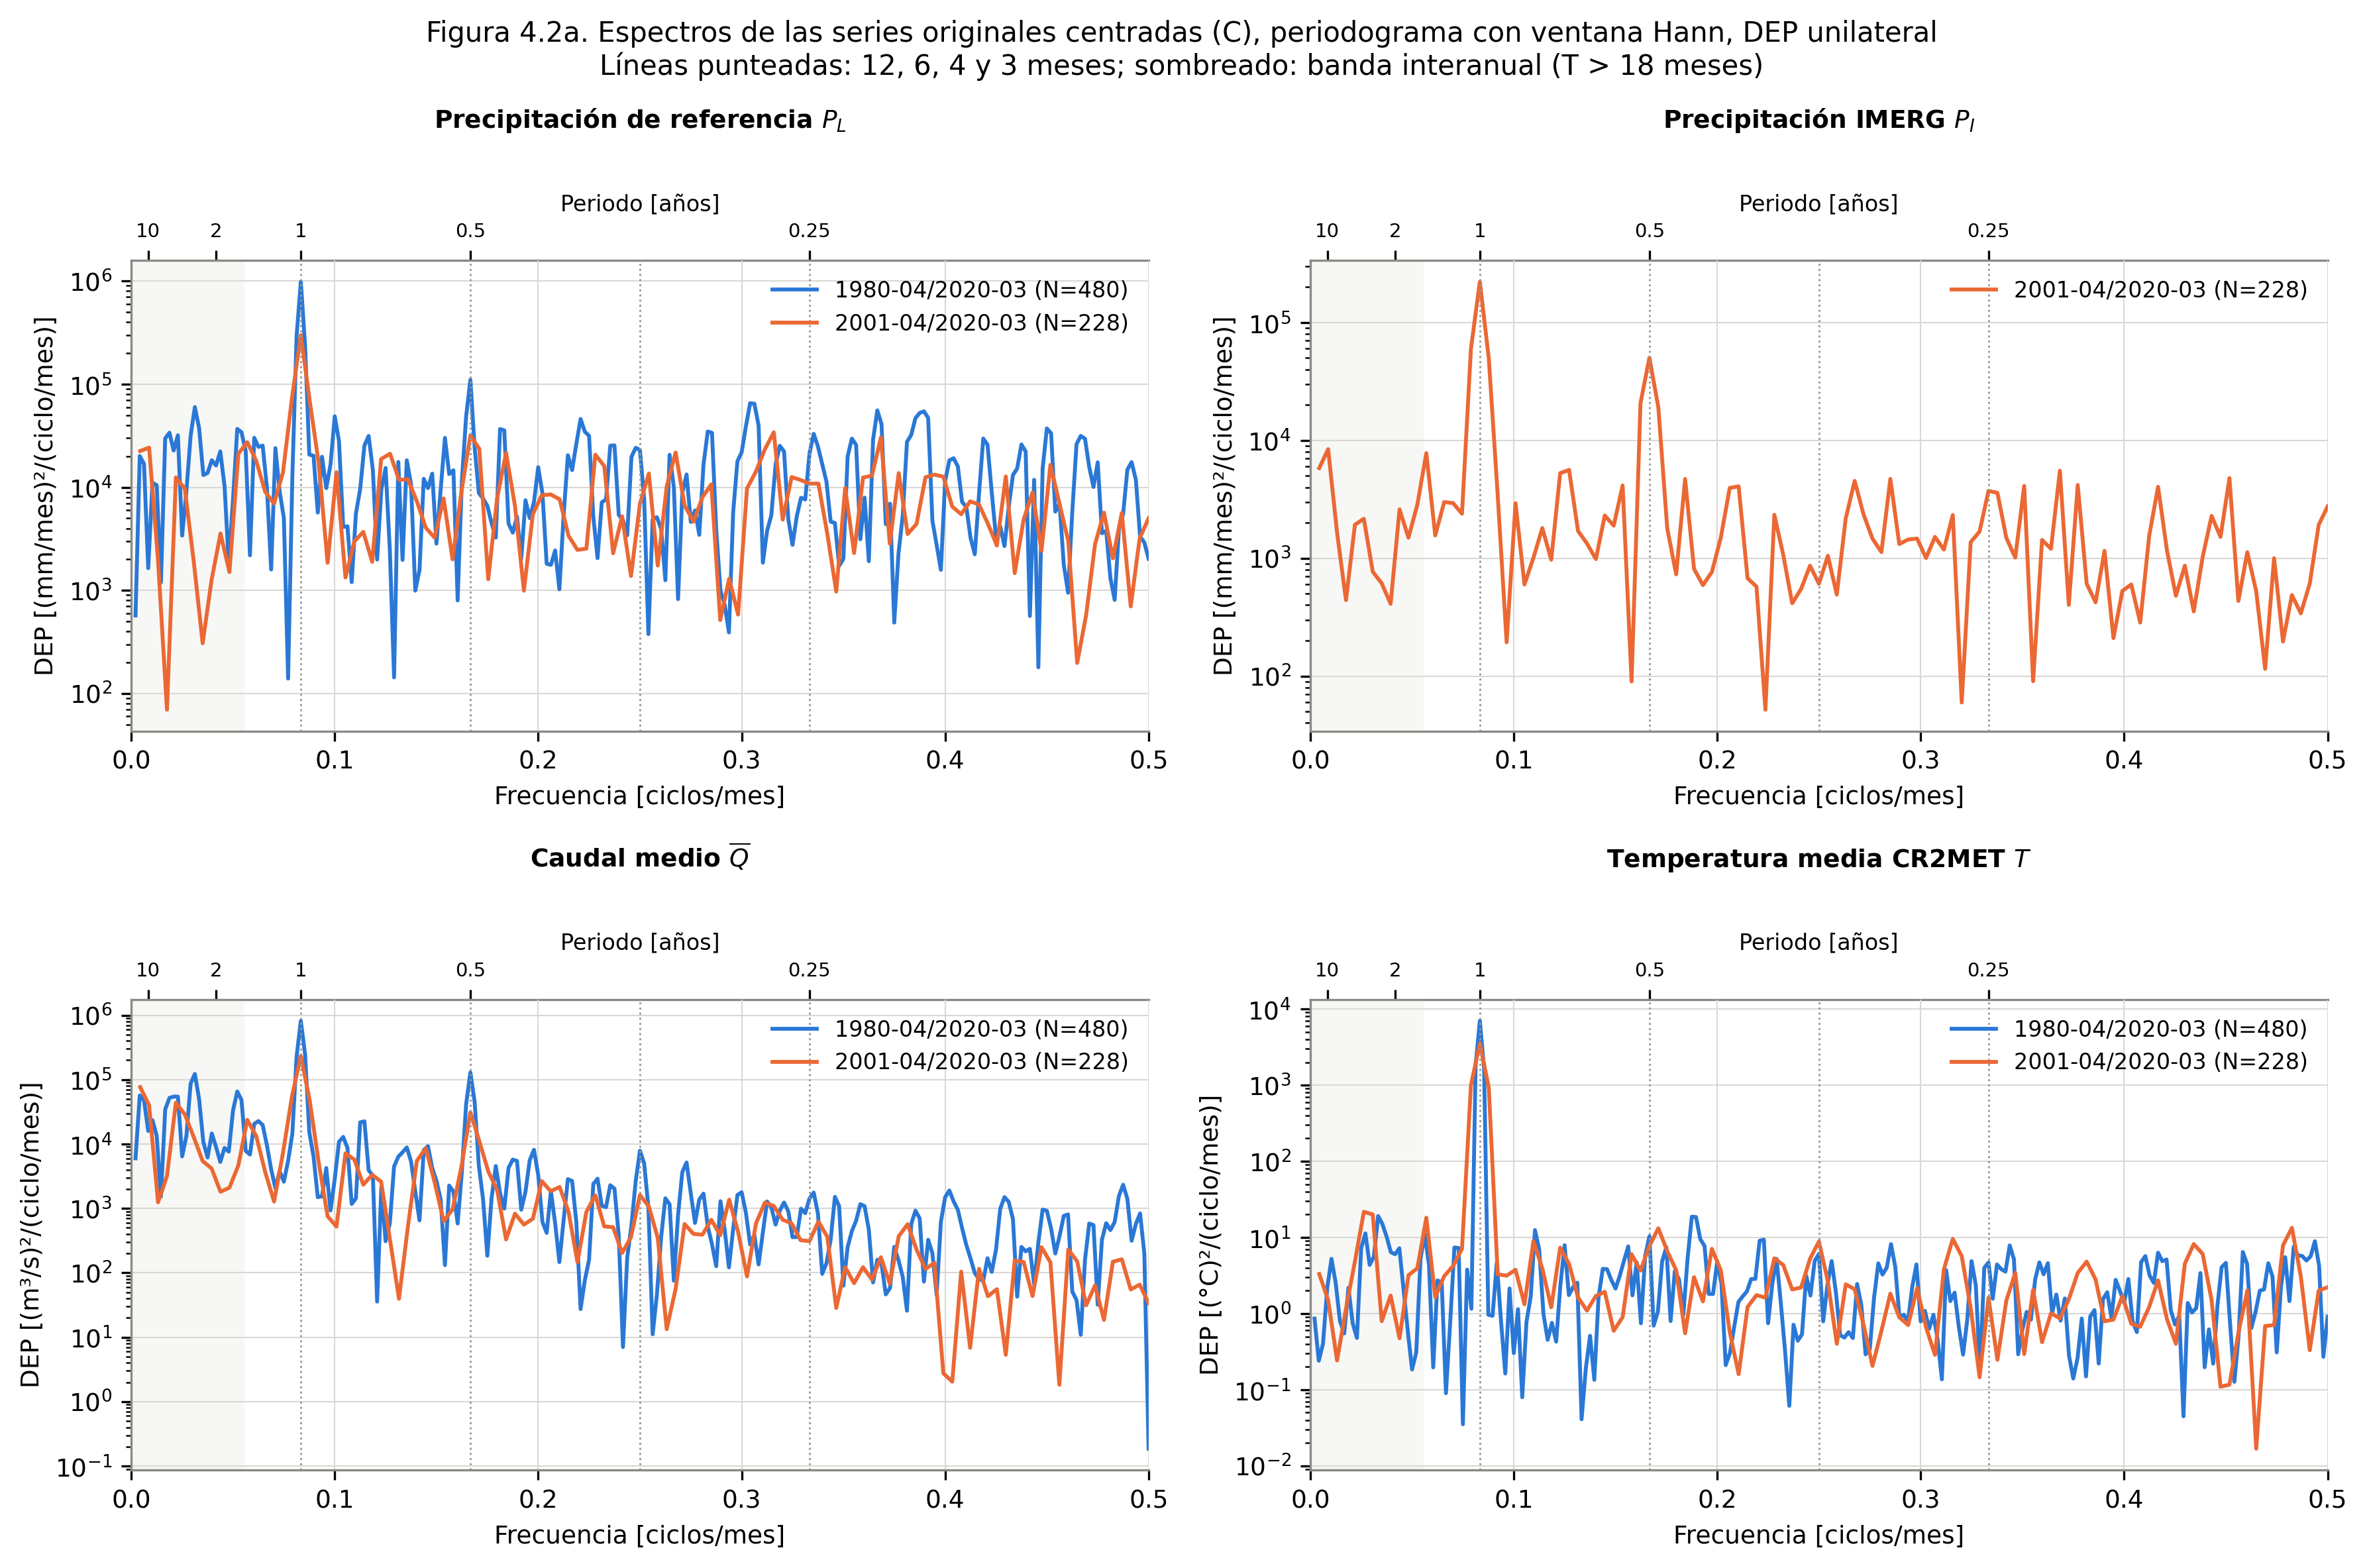
\includegraphics[width=0.92\textwidth]{figura_4_2a_espectros_originales.png}
\caption{Espectros de las series originales centradas (C), periodograma Hann, densidad espectral unilateral en (unidad)$^2$/(ciclo/mes). Eje superior: periodo en años. Líneas punteadas: 12, 6, 4 y 3 meses; sombreado: banda interanual ($T>18$ meses). Script \archivo{14_p4_2_espectros_interpretacion.py}.}
\label{fig:esporig}
\end{figure}

\begin{figure}[H]
\centering
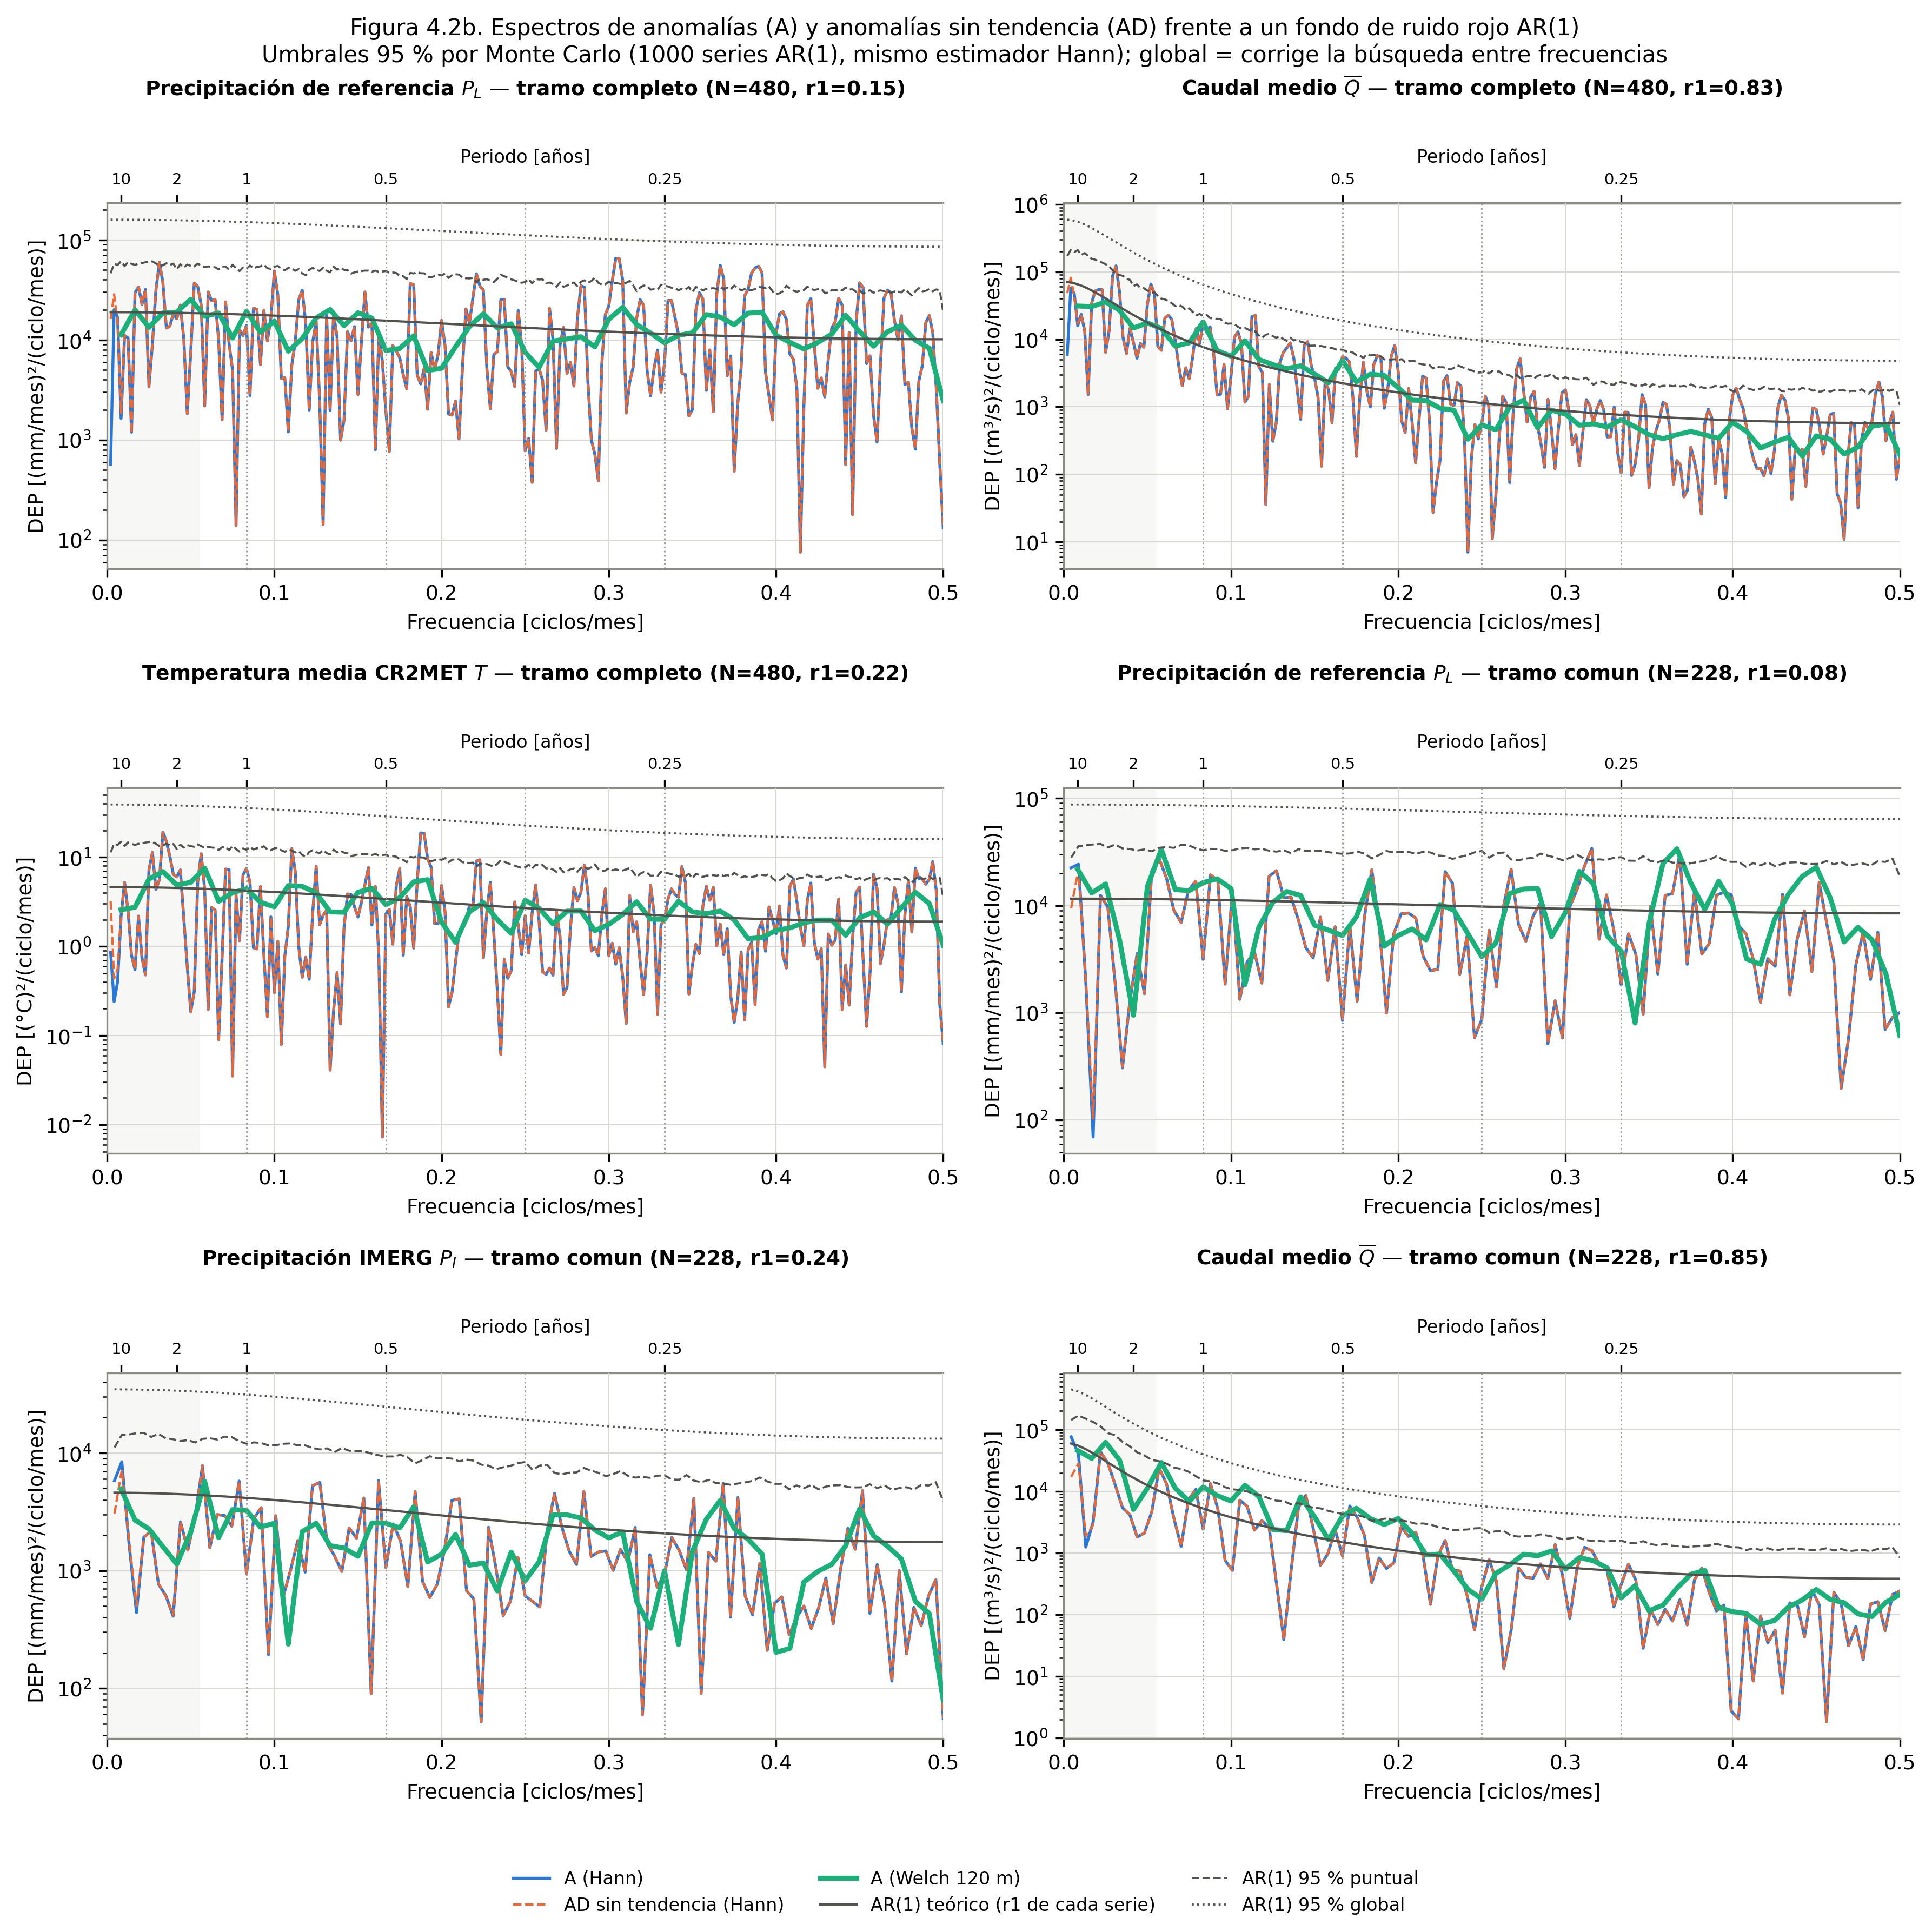
\includegraphics[width=0.92\textwidth]{figura_4_2b_espectros_anomalias_ar1.png}
\caption{Espectros de anomalías (A, azul), anomalías sin tendencia (AD, naranja) y Welch (verde) frente al fondo AR(1) (gris) y sus umbrales del 95\,\% puntual (discontinuo) y global (punteado), obtenidos con 1000 simulaciones.}
\label{fig:espanom}
\end{figure}

\begin{table}[H]
\centering\small
\caption{Fracción de la varianza por banda, periodograma Hann (\archivo{figuras/tabla_4_2_fracciones_banda.csv}). Interanual: periodos de más de 18 meses; anual: 10.5--14 meses; semianual: 5.25--7 meses; resto: frecuencias intraanuales no armónicas.}
\label{tab:bandas}
\begin{tabular}{lllrrrr}
\toprule
Variable & Tramo & Serie & Interanual & Anual & Semianual & Resto \\
\midrule
$\PL$ & 1980--2020 & C & 0.10 & 0.32 & 0.08 & 0.50 \\
$\Qm$ & 1980--2020 & C & 0.30 & 0.47 & 0.10 & 0.13 \\
$T$ & 1980--2020 & C & 0.01 & 0.94 & 0.01 & 0.04 \\
$\PL$ & 2001--2020 & C & 0.07 & 0.34 & 0.08 & 0.51 \\
$\PI$ & 2001--2020 & C & 0.05 & 0.55 & 0.17 & 0.23 \\
$\Qm$ & 2001--2020 & C & 0.30 & 0.47 & 0.09 & 0.14 \\
$T$ & 2001--2020 & C & 0.01 & 0.94 & 0.01 & 0.04 \\
\midrule
$\PL$ & 1980--2020 & A & 0.15 & 0.04 & 0.07 & 0.74 \\
$\Qm$ & 1980--2020 & A & 0.62 & 0.07 & 0.06 & 0.26 \\
$T$ & 1980--2020 & A & 0.17 & 0.06 & 0.15 & 0.62 \\
$\PL$ & 2001--2020 & A & 0.11 & 0.08 & 0.08 & 0.73 \\
$\PI$ & 2001--2020 & A & 0.15 & 0.08 & 0.13 & 0.65 \\
$\Qm$ & 2001--2020 & A & 0.57 & 0.10 & 0.07 & 0.25 \\
$T$ & 2001--2020 & A & 0.19 & 0.06 & 0.13 & 0.62 \\
\bottomrule
\end{tabular}
\end{table}

\begin{table}[H]
\centering\small
\caption{Picos espectrales principales, periodograma Hann (tabla completa en \archivo{figuras/tabla_4_2_picos_espectrales.csv}). El intervalo de periodo corresponde a $f\pm\Delta f$; ``Ciclos'' $=Nf$. AR(1): el pico supera el umbral del 95\,\% puntual (P) o global (G).}
\label{tab:picos}
\resizebox{\textwidth}{!}{\begin{tabular}{llllrrl}
\toprule
Variable & Tramo & Serie & Periodo [meses] & Intervalo & Ciclos & AR(1) \\
\midrule
$\PL$, $\Qm$, $\PI$, $T$ & ambos & C & 12.0 & 11.4--12.7 & 19--40 & no aplica (determinista) \\
$\PL$, $\PI$ & ambos & C & 6.0 & 5.8--6.2 & 38--80 & no aplica (armónico) \\
$\Qm$ & 1980--2020 & C & 240 & 160--480 & 2 & no aplica (tendencia) \\
$\PL$ & 1980--2020 & A & 32.0 & 30.0--34.3 & 15 & P, no G \\
$\Qm$ & 1980--2020 & A & 32.0; 19.2 & 30.0--34.3; 18.5--20.0 & 15; 25 & P, no G \\
$T$ & 1980--2020 & A & 30.0; 9.1; 5.3 & 28.2--32.0; 8.9--9.2; 5.3--5.4 & 16; 53; 90 & P, no G \\
$\Qm$ & 2001--2020 & A & 6.9 & 6.7--7.1 & 33 & P, no G \\
$T$ & 2001--2020 & A & 38.0; 17.5; 2.1 & 32.6--45.6; 16.3--19.0; 2.05--2.09 & 6; 13; 110 & P, no G; P y G en 2.1 \\
\bottomrule
\end{tabular}}
\end{table}

\paragraph{Bandas dominantes en las series originales.} En las cuatro variables domina la banda anual, el único pico inequívoco del análisis: 40 ciclos en el registro completo y varios órdenes de magnitud sobre el fondo. Su peso varía mucho. Reúne el 94\,\% de la varianza en $T$, cuyo ciclo casi sinusoidal sigue a la radiación; el 47\,\% en $\Qm$; el 55\,\% en $\PI$; y solo el 32--34\,\% en $\PL$. La precipitación de referencia concentra la mitad de su varianza en frecuencias intraanuales no armónicas, porque llega en pocos eventos frontales muy irregulares. El pico de 6 meses no indica un segundo proceso: es el armónico de un ciclo anual no sinusoidal, con un invierno lluvioso corto y un verano casi seco. Es más intenso en $\PI$ (17\,\%) que en $\PL$ (8--9\,\%), porque IMERG reproduce un ciclo más regular y menos variabilidad entre eventos, coherente con su subestimación de los extremos (punto 2).

\paragraph{Al retirar la climatología.} Las bandas anual y semianual se reducen al 4--10\,\% de la varianza de las anomalías. Lo que queda refleja que la amplitud del ciclo cambia de un año a otro, no un ciclo determinista. La varianza se redistribuye de forma muy distinta según la variable:
\begin{itemize}
\item $\PL$ y $\PI$ tienen espectros de anomalías casi planos, propios de un ruido casi blanco: $r_1=0.15$ y 0.24, con pendiente log--log de $+0.18$ y $-0.08$ para $f<1/12$. La banda interanual reúne solo el 11--15\,\% de la varianza.
\item $\Qm$ tiene un espectro \emph{rojo}: $r_1=0.83$ (0.85 en el periodo común), pendiente log--log de $-0.33$ a $-0.69$ y 57--62\,\% de la varianza en periodos de más de 18 meses, con poca potencia en altas frecuencias (Figura~\ref{fig:espnorm}).
\item $T$ tiene una persistencia débil ($r_1=0.22$ en 40 años y 0.27 en el periodo común) y un 17--19\,\% de varianza interanual: sus anomalías mensuales dependen de la circulación del mes y no se acumulan.
\end{itemize}

\begin{figure}[H]
\centering
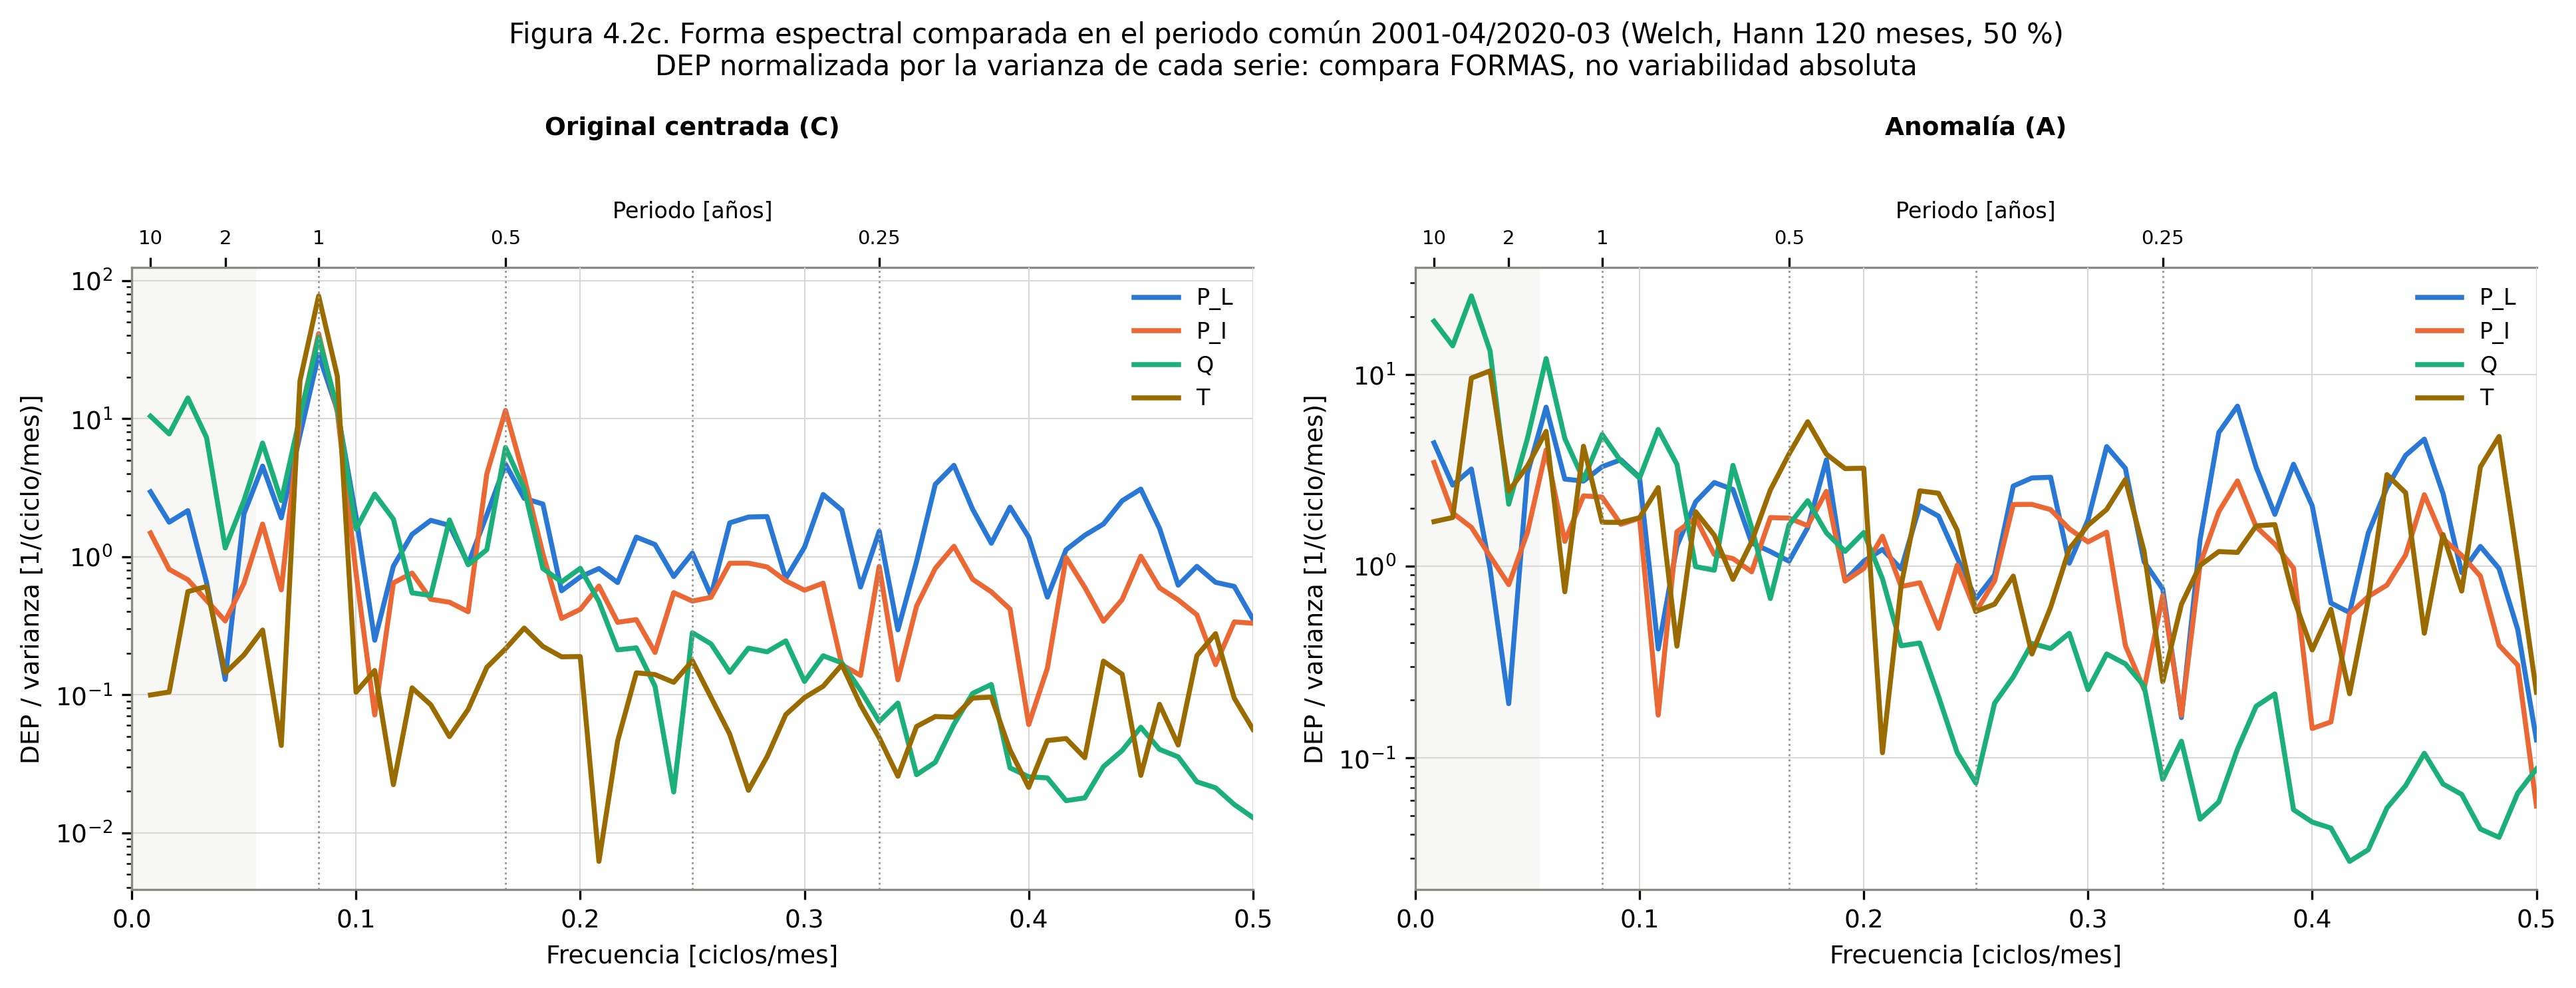
\includegraphics[width=0.95\textwidth]{figura_4_2c_espectros_normalizados.png}
\caption{Forma espectral comparada en el periodo común (Welch). Densidad normalizada por la varianza de cada serie: se comparan formas, no variabilidad absoluta.}
\label{fig:espnorm}
\end{figure}

\paragraph{Almacenamiento y persistencia.} El contraste entre la lluvia, con anomalías casi blancas, y el caudal, con un espectro rojo, es la evidencia espectral más clara del punto 4 y confirma la hipótesis H-c. La cuenca actúa como un filtro pasa-bajos: atenúa las variaciones de uno a pocos meses y traslada la varianza a escalas interanuales. Es lo esperable en un sistema que integra la lluvia de varios meses en la nieve, los glaciares y el agua subterránea y la libera de forma suavizada \citep{AlvarezGarreton2021,Ayala2020}. La regulación del embalse El Yeso también suaviza el caudal; sin datos de operación no podemos separar ambos efectos, aunque la magnitud del enrojecimiento (de $r_1=0.15$ a 0.83) y un índice de flujo base de 0.81 sugieren un control natural dominante. Un espectro de potencia no contiene la fase entre dos series, así que el desfase lluvia--caudal no se infiere de estas figuras: proviene de la climatología (punto 1) y de los rezagos (punto 2).

\begin{table}[H]
\centering\small
\caption{Sensibilidad del periodo interanual dominante y de la fracción interanual de las anomalías (\archivo{figuras/tabla_4_2_estabilidad_picos.csv}).}
\label{tab:estab4}
\resizebox{\textwidth}{!}{\begin{tabular}{llrr}
\toprule
Variable & Configuración & Periodo dominante [años] & Fracción interanual \\
\midrule
$\PL$ & Hann / boxcar / Welch, 1980--2020 & 2.7 / 20.0 / 1.7 & 0.15 / 0.18 / 0.14 \\
$\PL$ & 1980--2000 / 2000--2020 & 1.7 / 1.5 & 0.14 / 0.13 \\
$\PL$ & sin tendencia / winsorizada & 2.7 / 2.7 & 0.16 / 0.16 \\
$\Qm$ & Hann con relleno / continua 1993-06--2007-09 / Lomb--Scargle & 2.7 / 2.4 / 20.0 & 0.62 / 0.60 / 0.61 \\
$\Qm$ & Welch, 120 meses & 3.3 & 0.55 \\
$\Qm$ & 1980--2000 / 2000--2020 & 5.0 / 20.0 & 0.56 / 0.59 \\
$\Qm$ & sin tendencia / winsorizada & 2.7 / 2.7 & 0.64 / 0.63 \\
$T$ & Hann / boxcar / Welch, 1980--2020 & 2.5 / 2.5 / 2.5 & 0.17 / 0.17 / 0.16 \\
$T$ & 1980--2000 / 2000--2020 & 1.8 / 2.9 & 0.12 / 0.21 \\
\bottomrule
\end{tabular}}
\end{table}

\paragraph{Estabilidad y significancia.} Lo robusto es la \emph{forma} del espectro, no la ubicación de un pico interanual (Tabla~\ref{tab:estab4}). El periodo dominante salta de 2.7 años (Hann) a 20 años (boxcar, dominado por la fuga desde la frecuencia más baja) y a 1.7--3.3 años (Welch), y cambia entre las dos mitades del registro. Retirar la tendencia casi no cambia el registro completo, pero en el periodo común reduce la fracción interanual del caudal de 0.57 a 0.48: en 19 años, la caída de la megasequía aparece como potencia de muy baja frecuencia. Winsorizar los extremos, lo que incluye el mayo de 1993, no altera las fracciones, y el relleno de vacíos tampoco. \textbf{Ningún pico interanual supera el umbral global del AR(1)}. Los que superan el umbral puntual (32 meses en $\PL$ y $\Qm$, 19 meses en $\Qm$, 30 meses en $T$ y 38 y 17.5 meses en $T$ en el periodo común) son los esperables por azar al examinar cientos de frecuencias, tienen pocos ciclos y no se mantienen entre estimadores ni entre tramos. El único pico que supera el umbral global es de 2.1 meses en la temperatura del periodo común, junto a la frecuencia de Nyquist. No aparece en el registro de 40 años ni con Welch, y una alternancia de un mes a otro no tiene un mecanismo físico plausible; lo atribuimos al muestreo o al procesamiento del producto y no lo interpretamos. No afirmamos ninguna periodicidad interanual.

\begin{purplebox}[title={Conclusión del punto 4}]
La variabilidad mensual se concentra en dos escalas. (1) El \textbf{ciclo anual}, única periodicidad significativa y estable. Domina $T$ (94\,\%) por el forzamiento radiativo; en $\PL$ (32\,\%) refleja la estación de los sistemas frontales, ligada a la migración del anticiclón del Pacífico Sur \citep{Garreaud2009}; en $\Qm$ (47\,\%) es la respuesta nival desfasada. Su armónico de 6 meses describe la forma del ciclo, no un proceso independiente. (2) Una \textbf{banda interanual amplia, sin picos}, que en el caudal reúne el 62\,\% de la varianza de las anomalías por el filtrado del almacenamiento y que en la lluvia es débil (11--15\,\%). La banda de 2--7 años es compatible con la escala de ENSO \citep{Trenberth1997}, pero un pico interanual no basta para atribuirla a ENSO, y aquí ni siquiera hay un pico robusto: la conexión se evalúa en el punto 5. Los periodos de 20 años o más tienen 1--2 ciclos en el registro y no se distinguen de la tendencia del punto 3.
\end{purplebox}
\subsection{Punto 5. Mapas de correlación con el clima global}
\label{sec:p5}

\subsubsection{Campos climáticos (5.1)}

\begin{table}[H]
\centering\footnotesize
\caption{Campos climáticos utilizados (\archivo{figuras/tabla_5_1_metadatos_campos.csv}). Tipo \emph{monthly averaged reanalysis}; enero de 1979 a diciembre de 2020 (504 meses sin faltantes); malla global de 1$^\circ$ interpolada por el CDS a partir de 0.25$^\circ$. Archivos en \archivo{datos/campos_era5/}.}
\label{tab:campos}
\begin{tabularx}{\textwidth}{l>{\raggedright\arraybackslash}X l l >{\raggedright\arraybackslash}X}
\toprule
Campo & Producto CDS y variable & Unidades & Rango & Máscara \\
\midrule
SST & ERA5 \emph{single levels monthly means} \citep{ERA5single}, \texttt{sea\_surface\_temperature} & K $\rightarrow$ $^\circ$C & $-1.6$ a 36.3~$^\circ$C & Tierra y hielo marino (SST $\leq-1.6$~$^\circ$C); se excluyen celdas con algún año enmascarado \\
PNM & ídem, \texttt{mean\_sea\_level\_pressure} & Pa $\rightarrow$ hPa & 958.8 a 1048.5~hPa & Ninguna \\
Z500 & ERA5 \emph{pressure levels monthly means} \citep{ERA5pressure}, \texttt{geopotential} en 500~hPa & m$^2$\,s$^{-2}$ $\rightarrow$ m ($\Phi/g_0$) & 4655 a 5969~m & Ninguna \\
\bottomrule
\end{tabularx}
\end{table}

Incluimos 1979 para poder usar rezagos (enero de 1980 con $\ell=1$ se empareja con diciembre de 1979). Del lado de la cuenca, $\PL$ y $\Qm$ aportan 37--41 años por mes calendario; IMERG aporta solo 19--20, por lo que se usa como contraste de sensibilidad a la fuente. La SST de ERA5 es un producto de reanálisis forzado por análisis de SST observada; para que los resultados no dependan de ese producto, los contrastamos con NOAA ERSST v5 del catálogo de NOAA PSL sugerido en la guía (Sección~\ref{sec:ersst}). La Figura~\ref{fig:clim5} muestra la climatología invernal y la variabilidad interanual de cada campo: la de la SST es máxima en el Pacífico ecuatorial oriental (ENSO), y la de la PNM y la Z500 en las latitudes altas del Pacífico sur.

\begin{figure}[H]
\centering
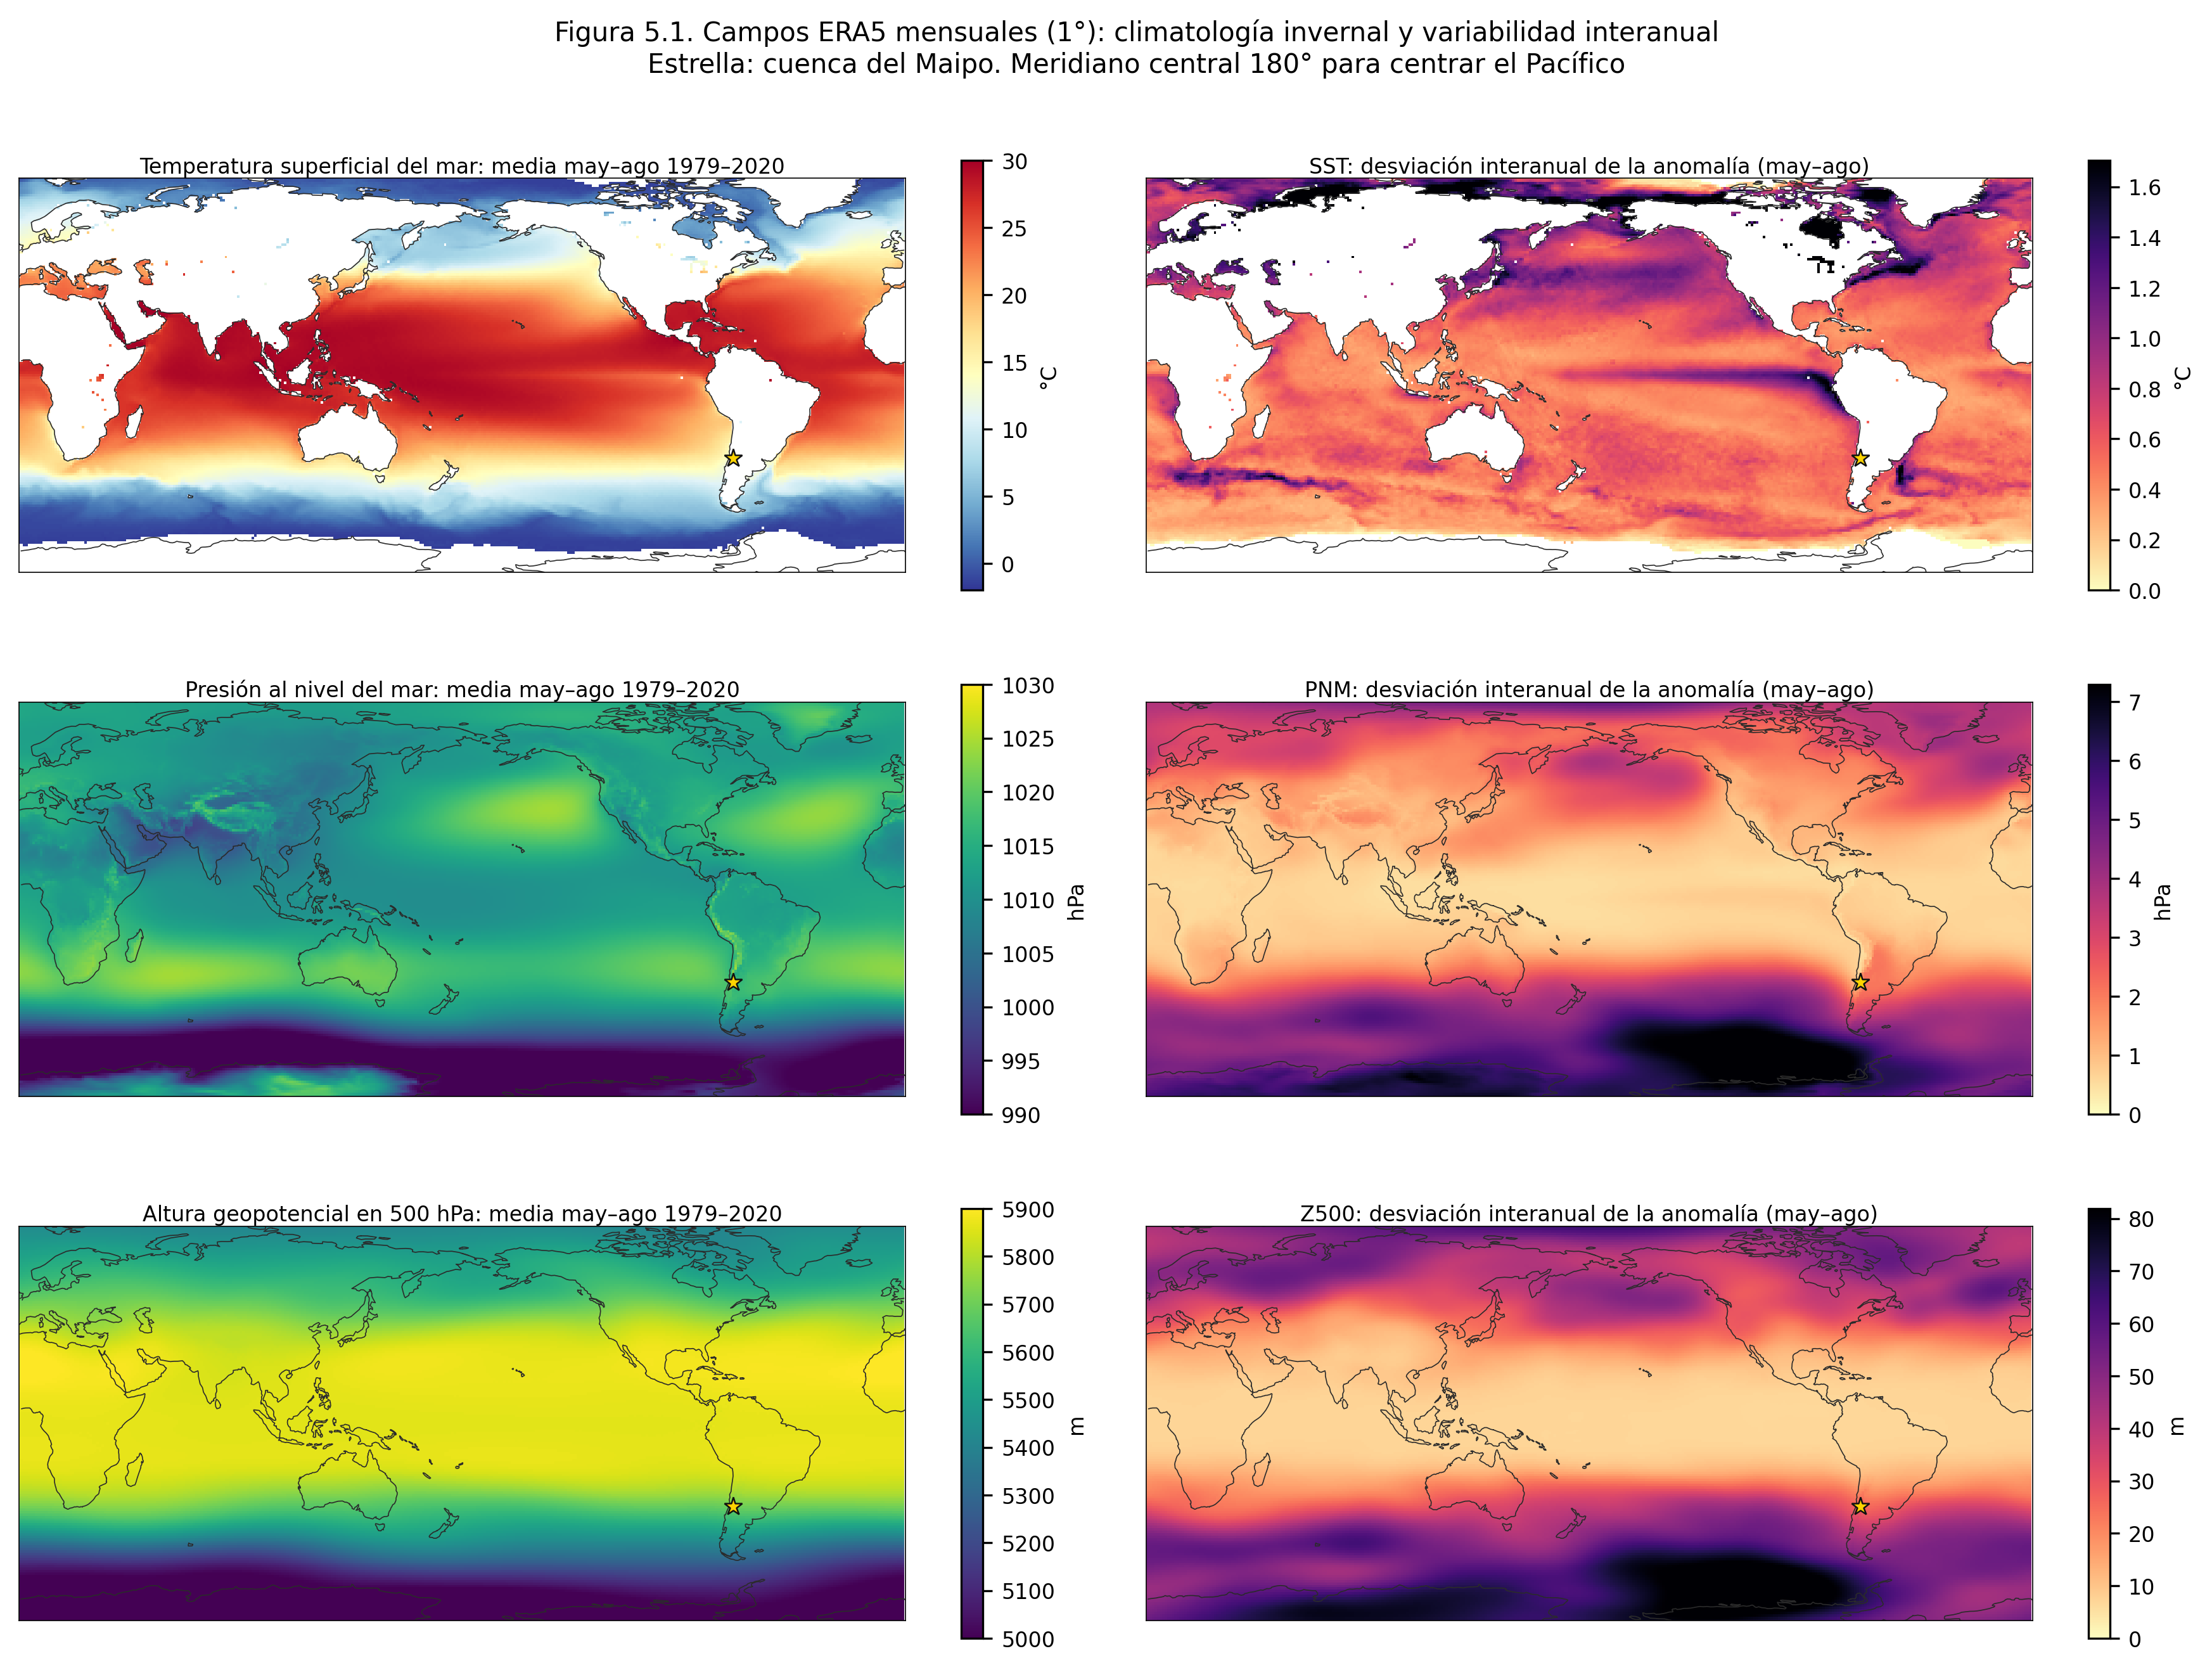
\includegraphics[width=0.92\textwidth]{figura_5_1_climatologia_campos.png}
\caption{Climatología de mayo a agosto (izquierda) y desviación estándar interanual de la anomalía (derecha) de SST, PNM y Z500. Estrella: cuenca. Script \archivo{16_p5_1_campos_climaticos.py}.}
\label{fig:clim5}
\end{figure}

\subsubsection{Mapas mensuales (5.2)}

Para cada combinación de variable de la cuenca y campo construimos doce mapas, uno por mes calendario de la respuesta de la cuenca, con escala divergente común de $-1$ a 1, la cuenca marcada y la significancia FDR punteada (Figuras~\ref{fig:pl_sst} a \ref{fig:lag6}). Como centrar o estandarizar con constantes positivas no cambia Pearson para un mes fijo, los mapas de valores originales y de anomalías son idénticos y mostramos una sola versión. Además del mapa base sin rezago ($\ell=0$) evaluamos un rezago justificado físicamente: el caudal frente a la SST seis meses antes, porque el deshielo depende de la nieve del invierno anterior.

\begin{figure}[H]
\centering
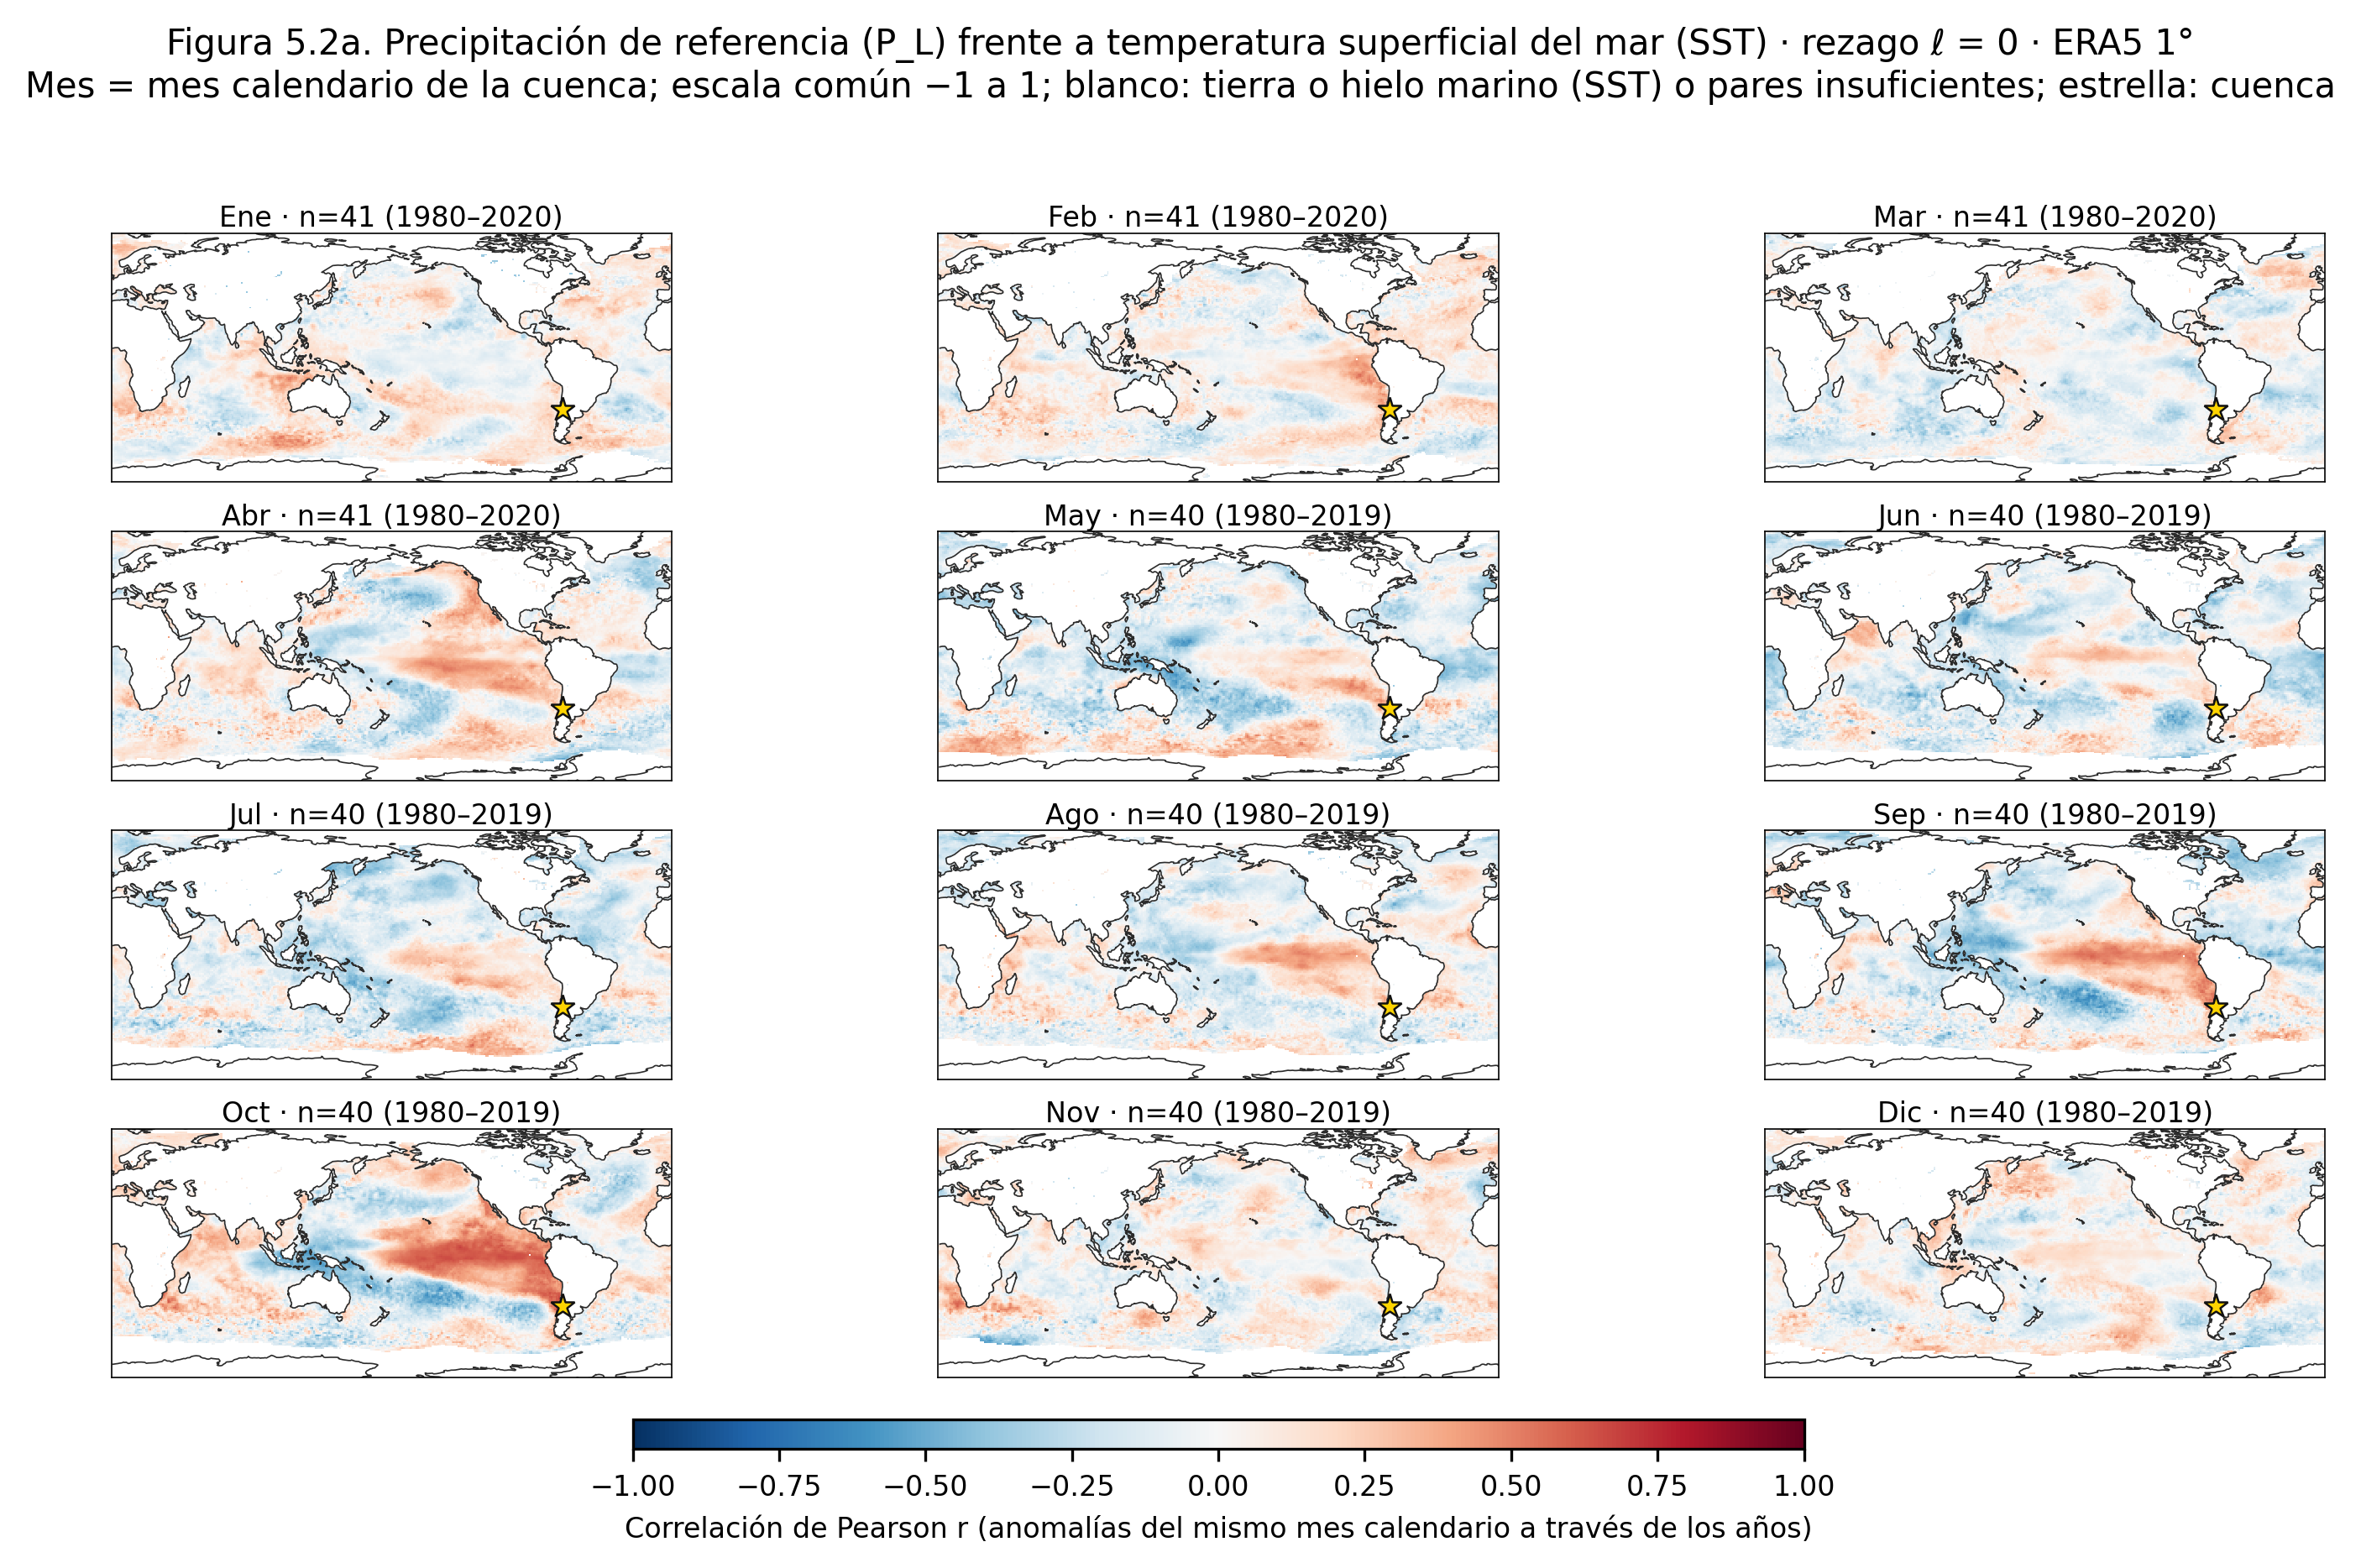
\includegraphics[width=0.88\textwidth]{figura_5_2a_p_l_sst.png}
\caption{$\PL$ frente a SST, $\ell=0$, doce meses. Script \archivo{17_p5_2_mapas_correlacion.py}.}
\label{fig:pl_sst}
\end{figure}

\begin{figure}[H]
\centering
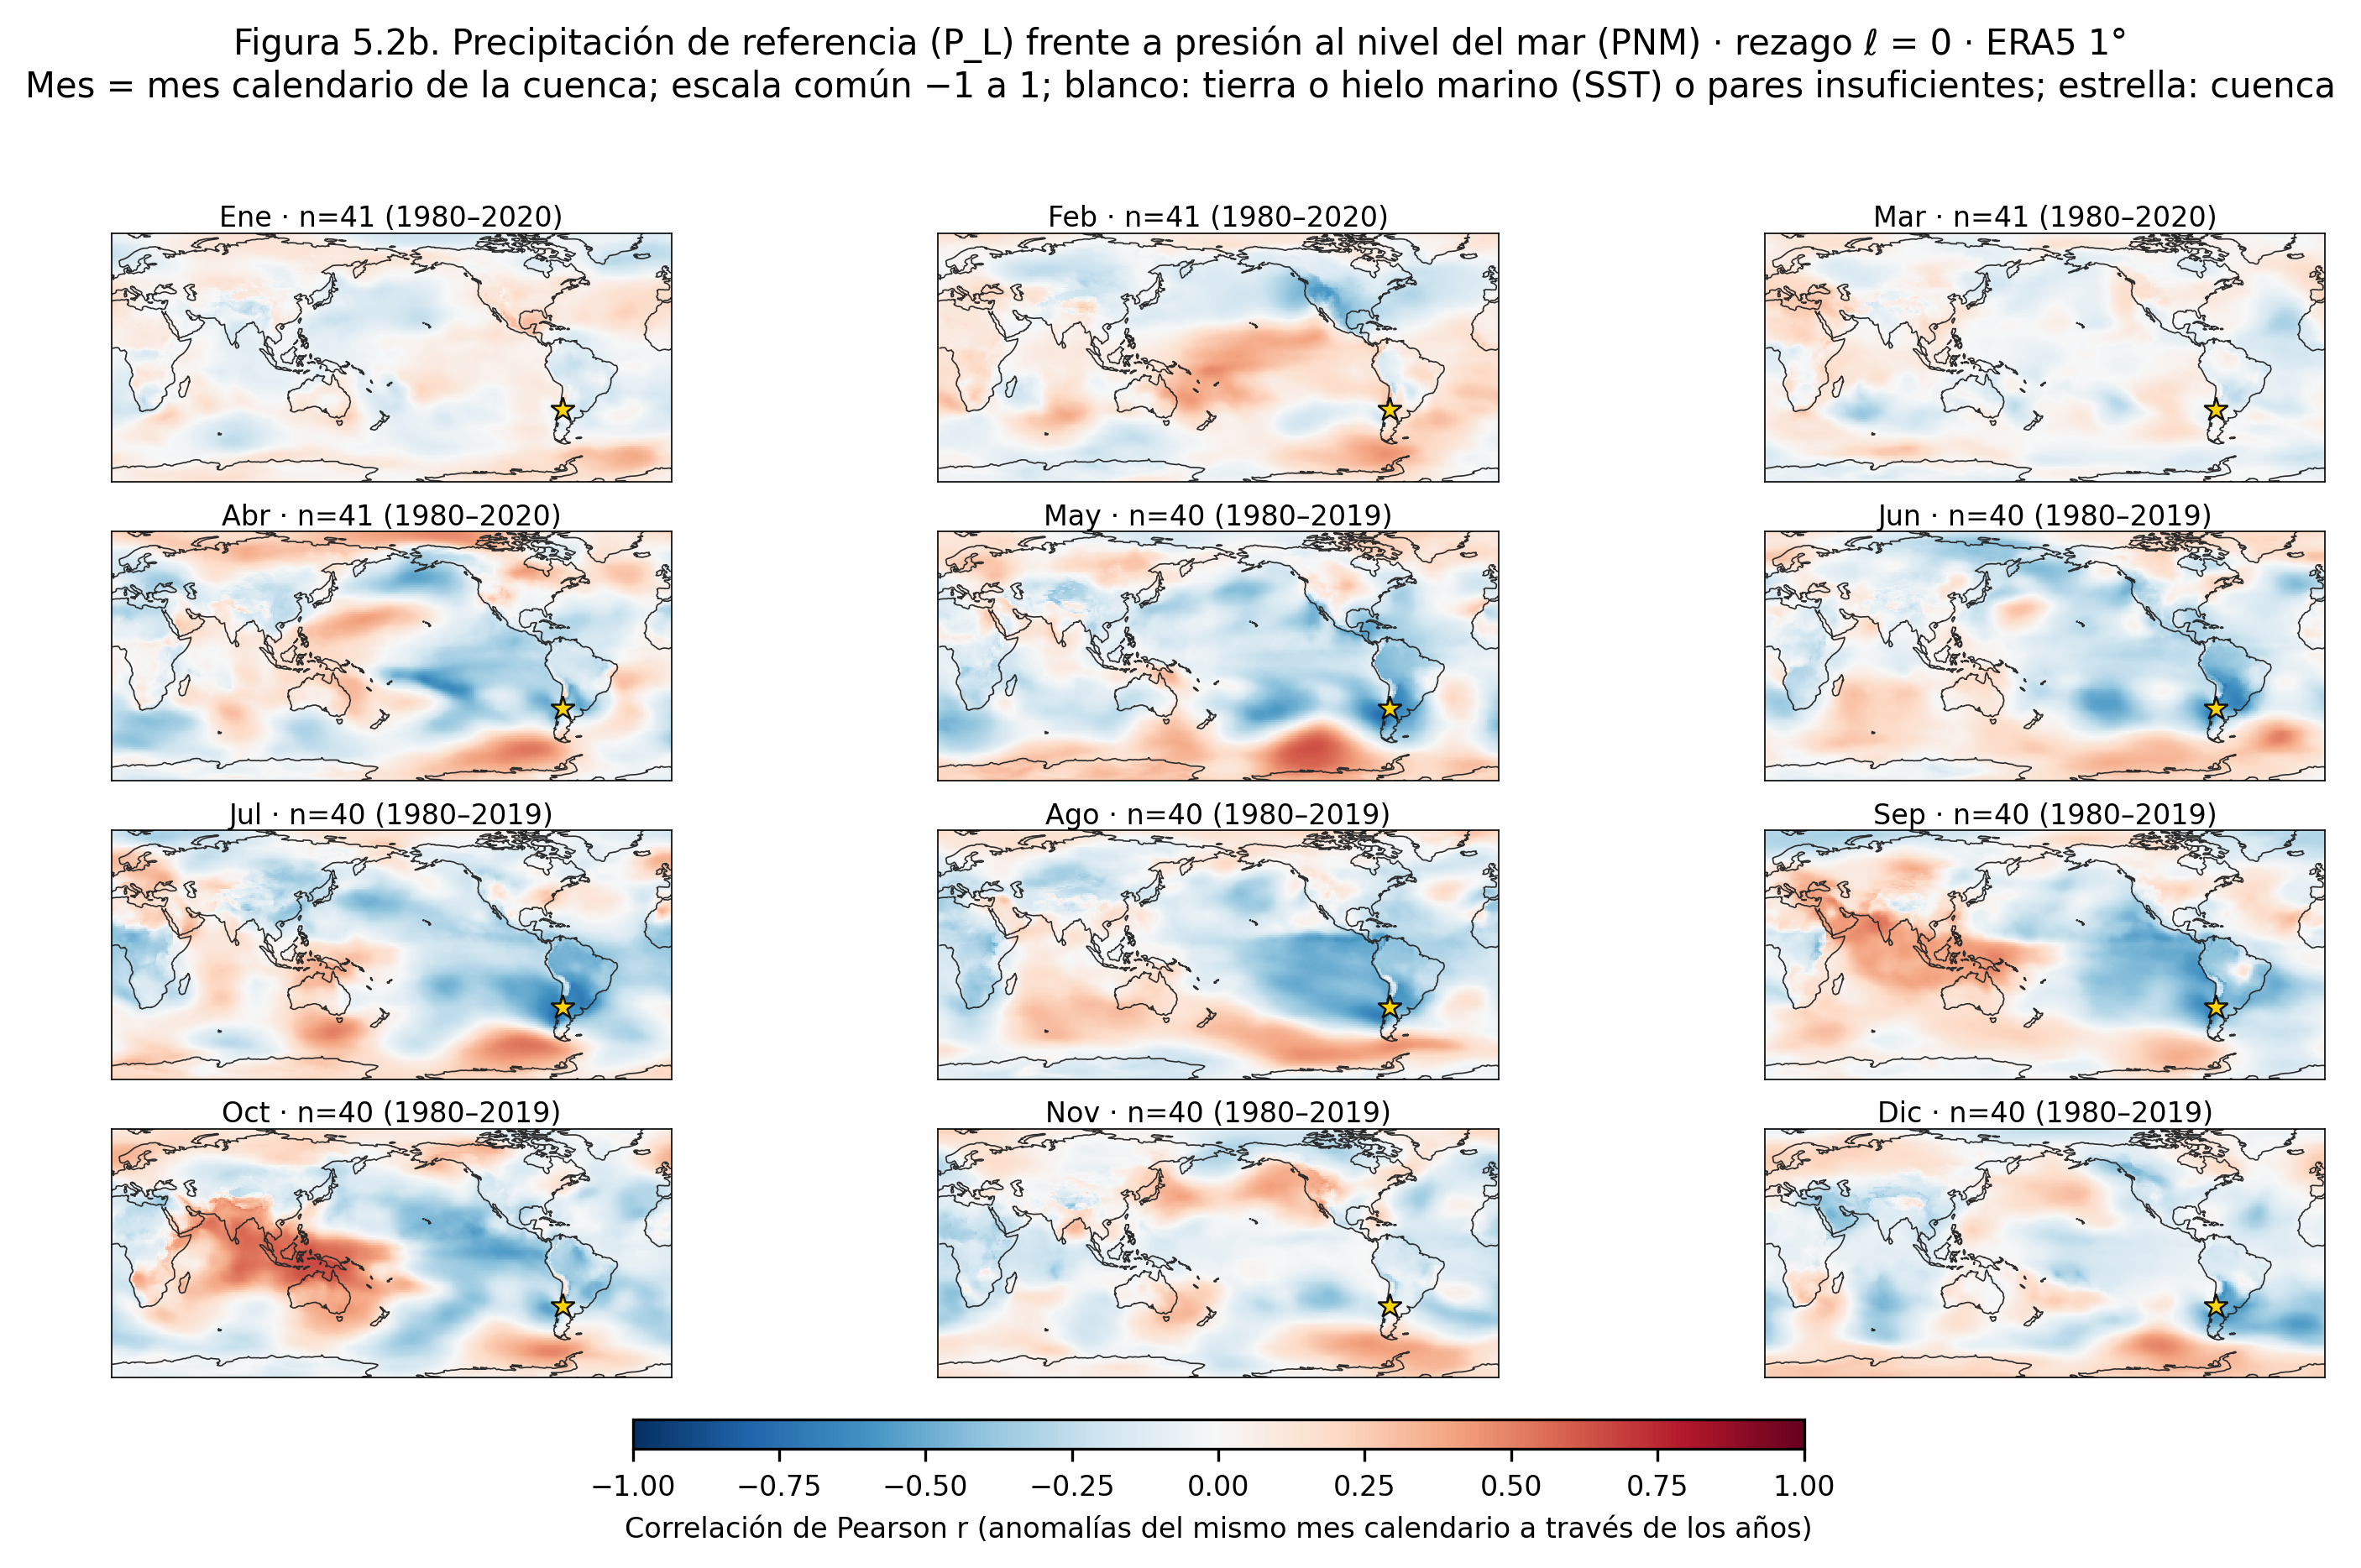
\includegraphics[width=0.88\textwidth]{figura_5_2b_p_l_msl.png}
\caption{$\PL$ frente a PNM, $\ell=0$.}
\label{fig:pl_msl}
\end{figure}

\begin{figure}[H]
\centering
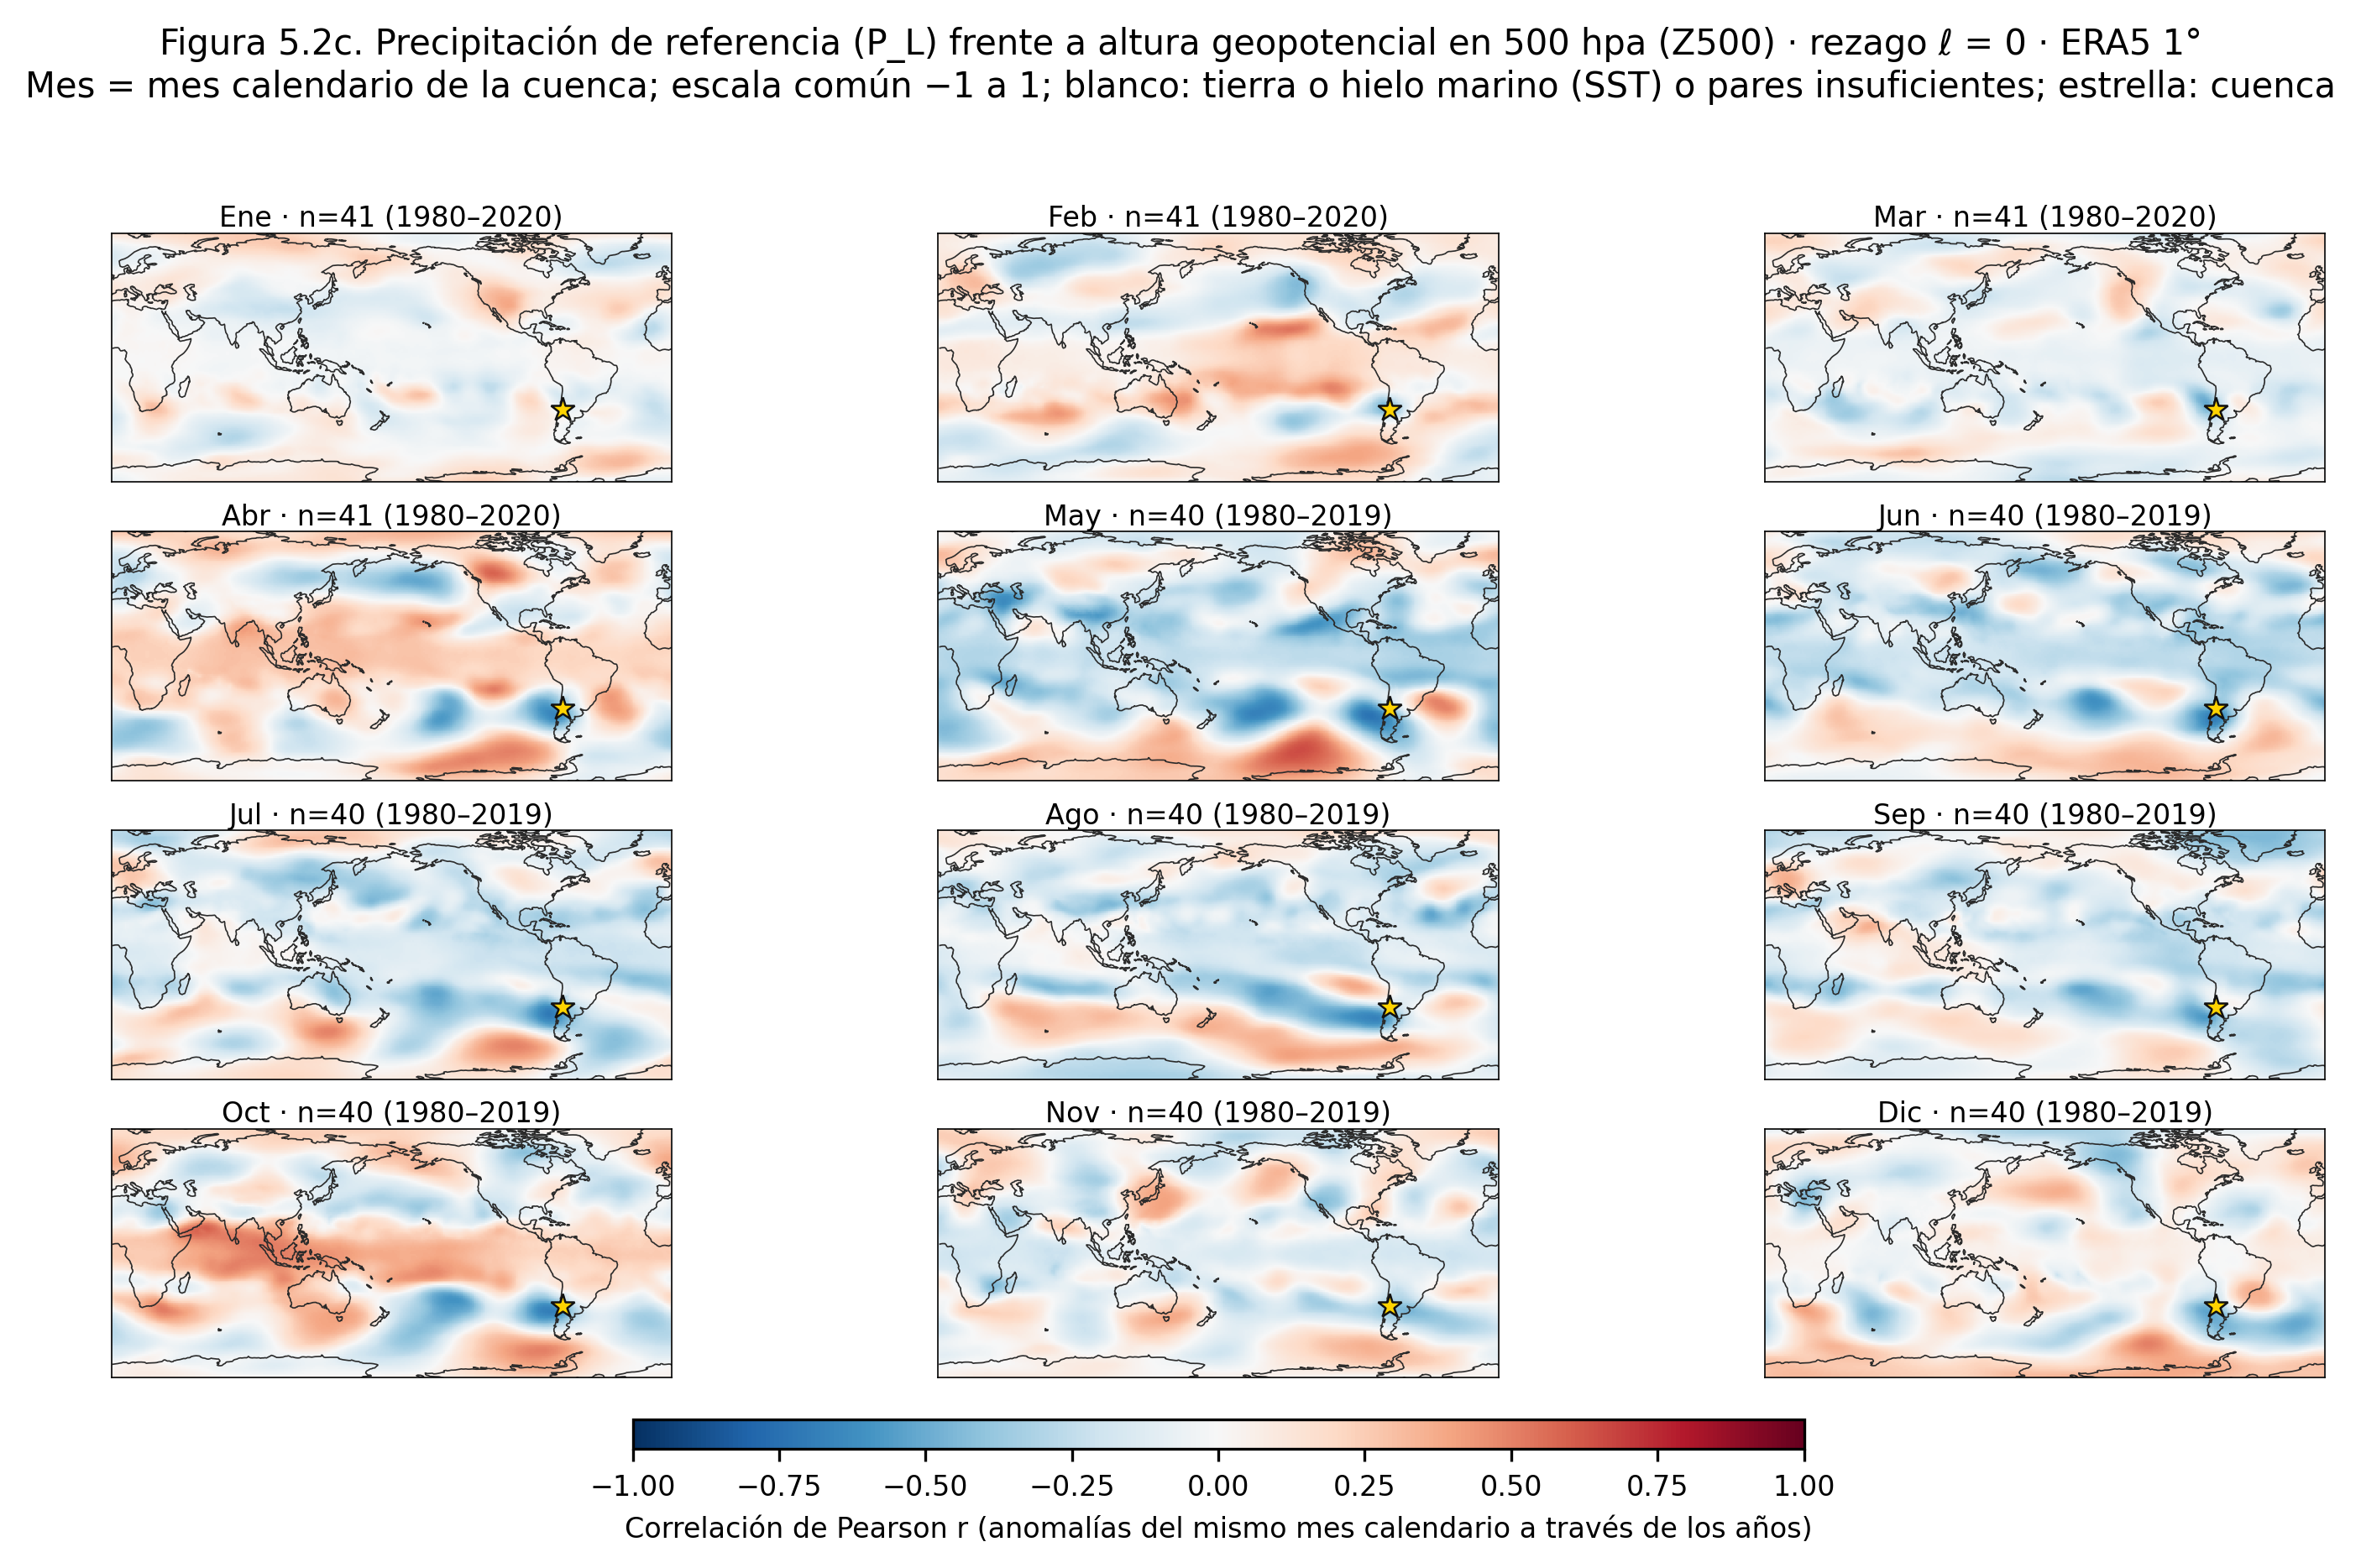
\includegraphics[width=0.88\textwidth]{figura_5_2c_p_l_z500.png}
\caption{$\PL$ frente a Z500, $\ell=0$.}
\label{fig:pl_z500}
\end{figure}

\begin{figure}[H]
\centering
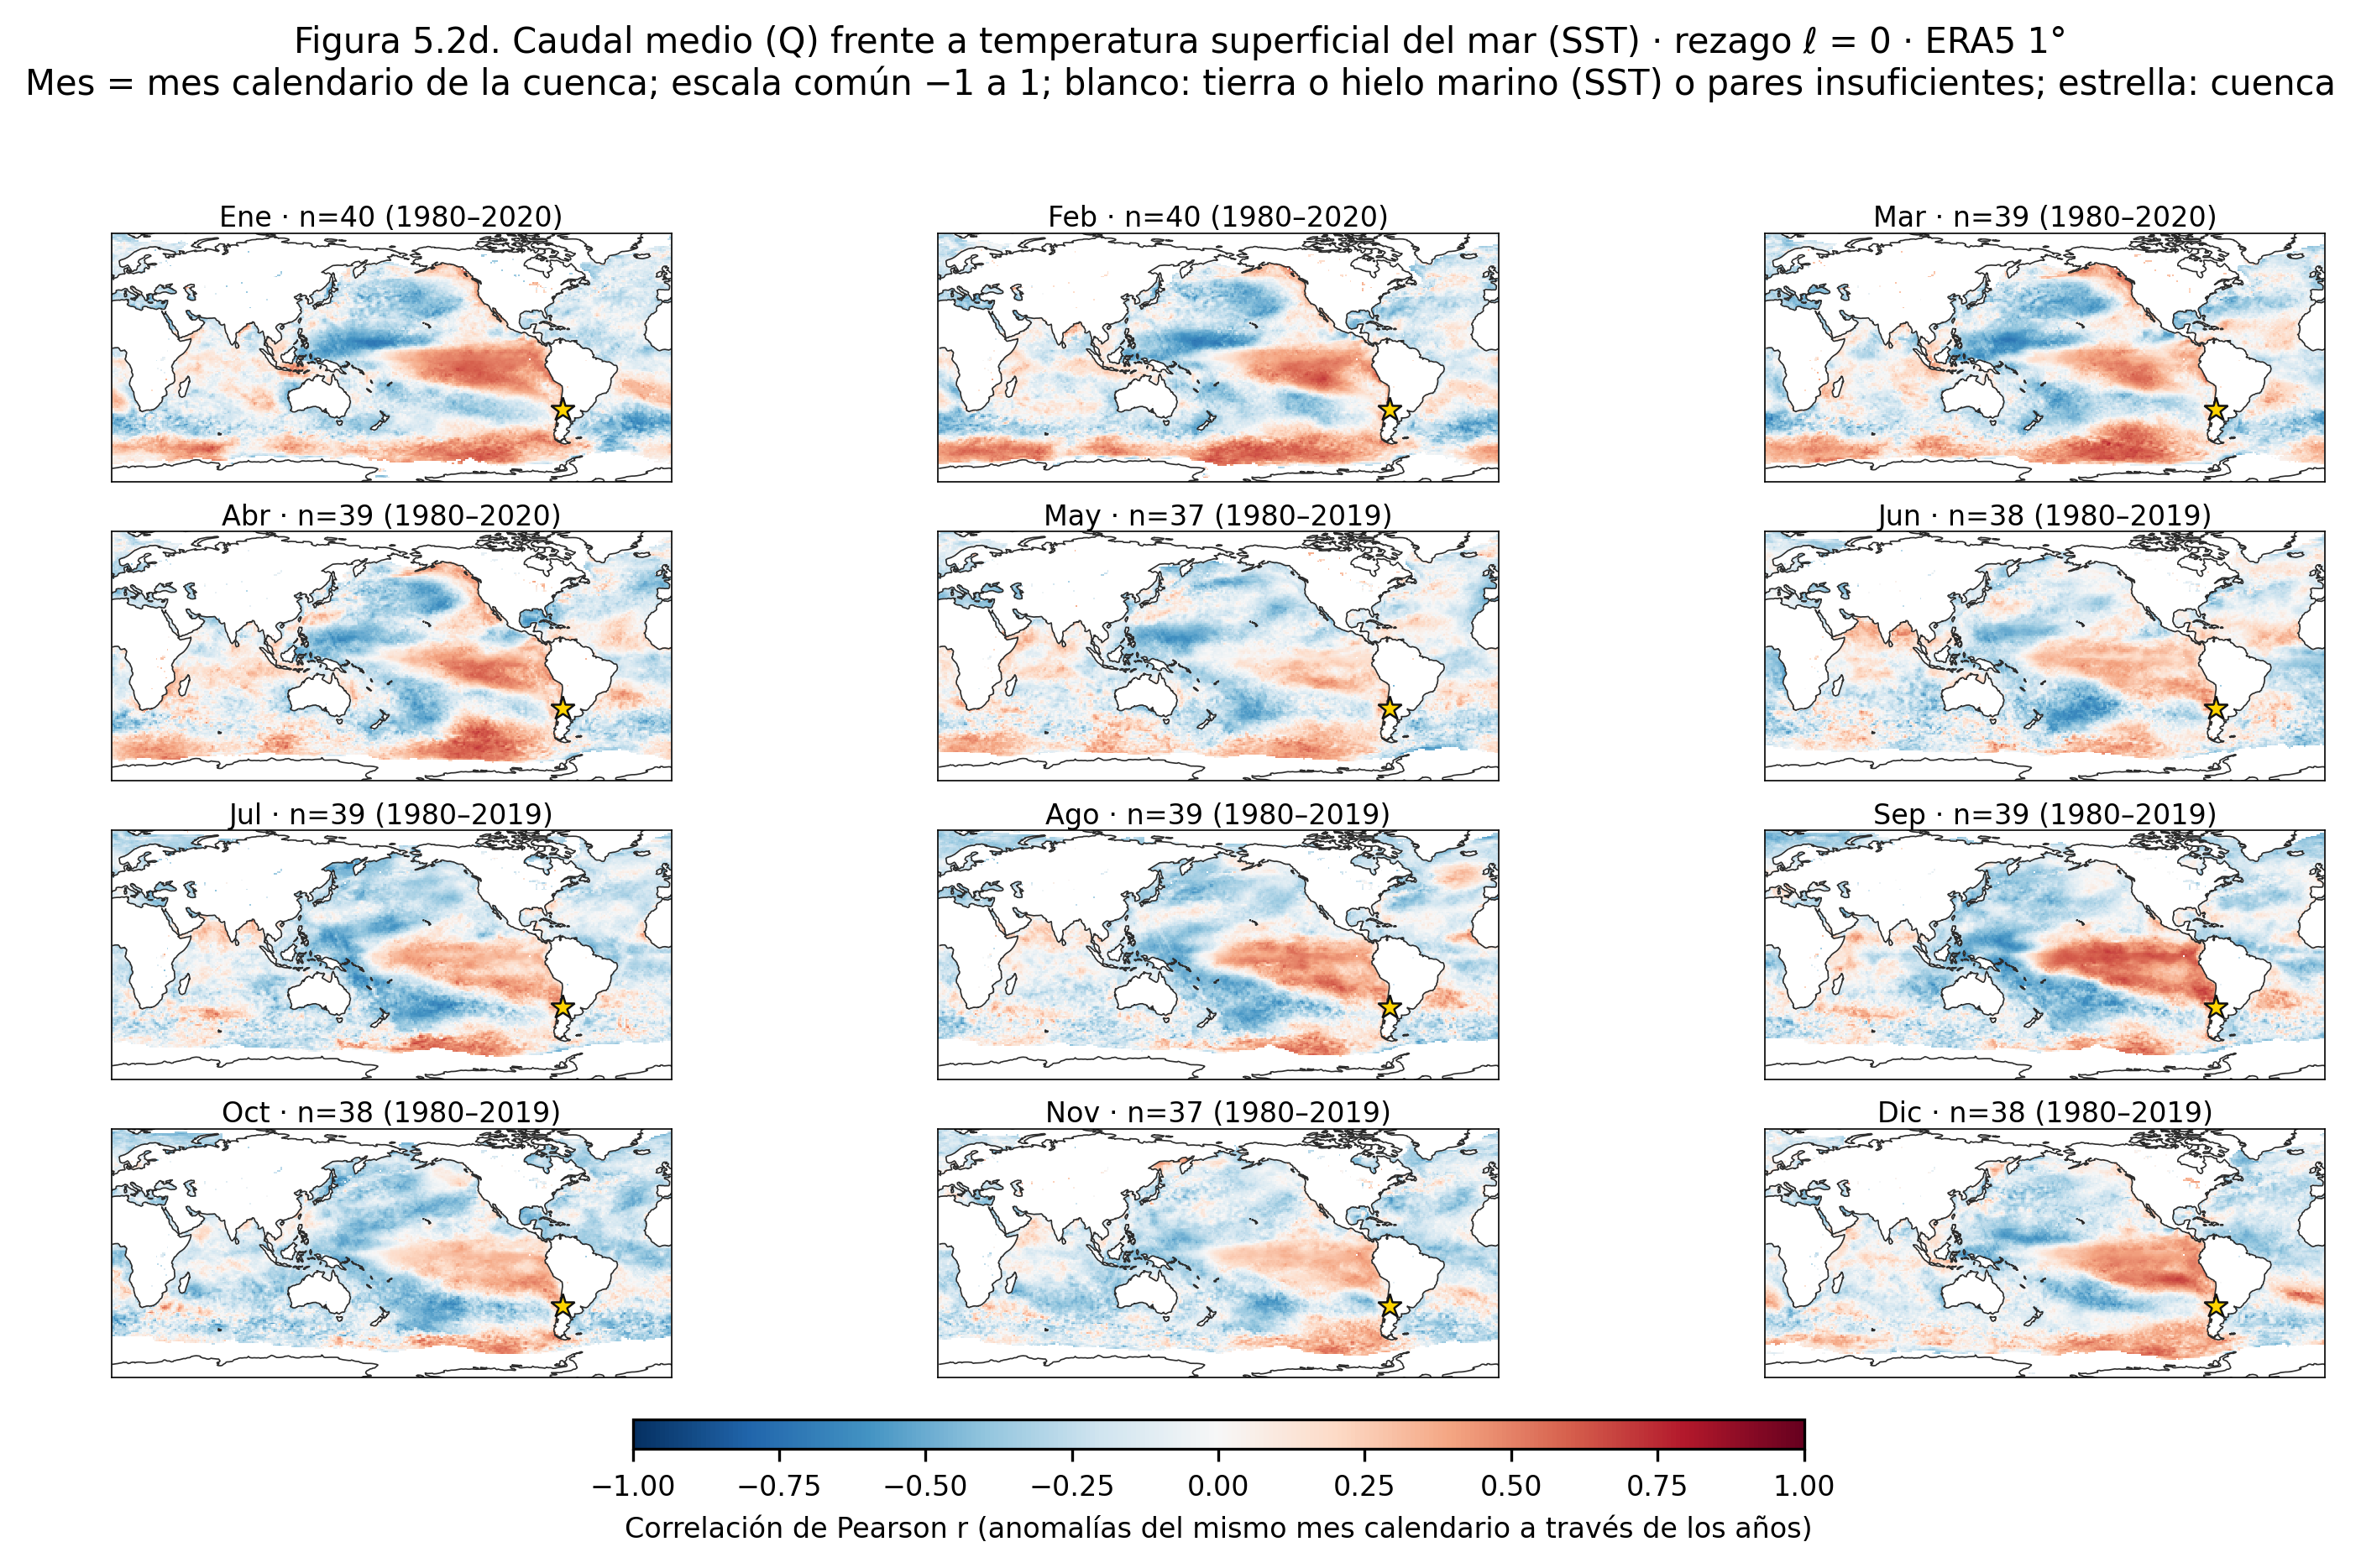
\includegraphics[width=0.88\textwidth]{figura_5_2d_q_sst.png}
\caption{$\Qm$ frente a SST, $\ell=0$.}
\label{fig:q_sst}
\end{figure}

\begin{figure}[H]
\centering
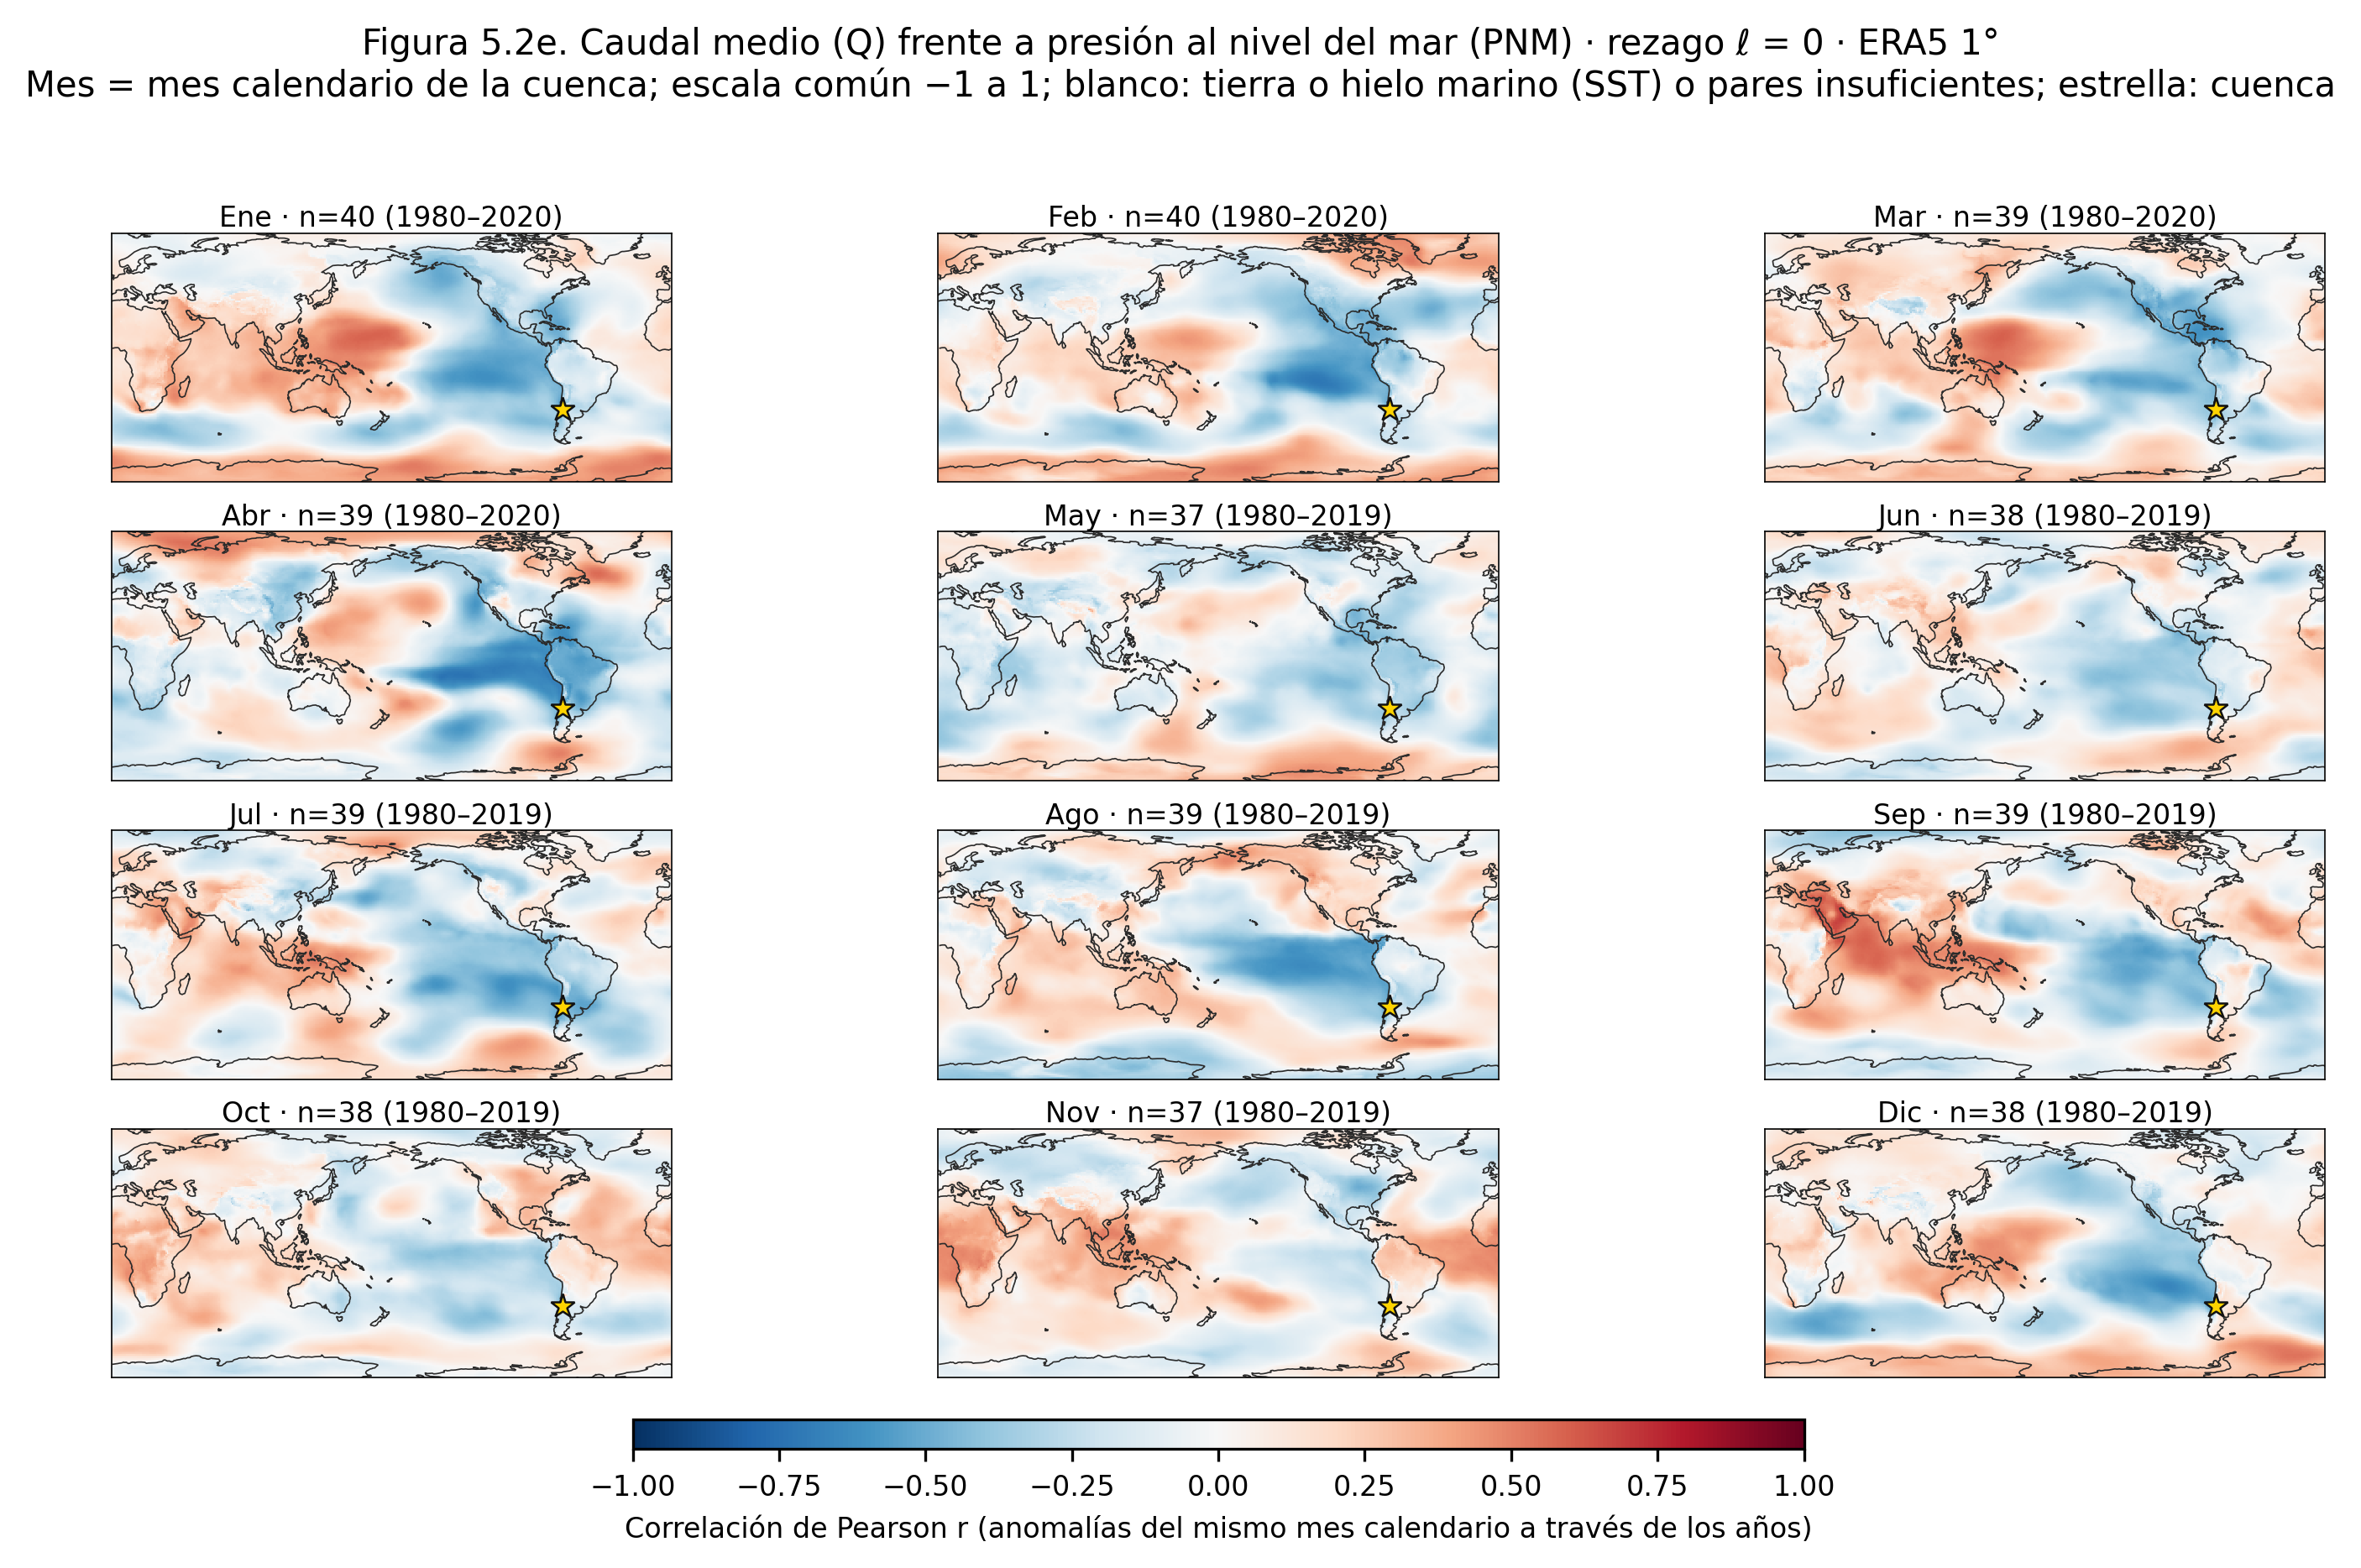
\includegraphics[width=0.88\textwidth]{figura_5_2e_q_msl.png}
\caption{$\Qm$ frente a PNM, $\ell=0$.}
\label{fig:q_msl}
\end{figure}

\begin{figure}[H]
\centering
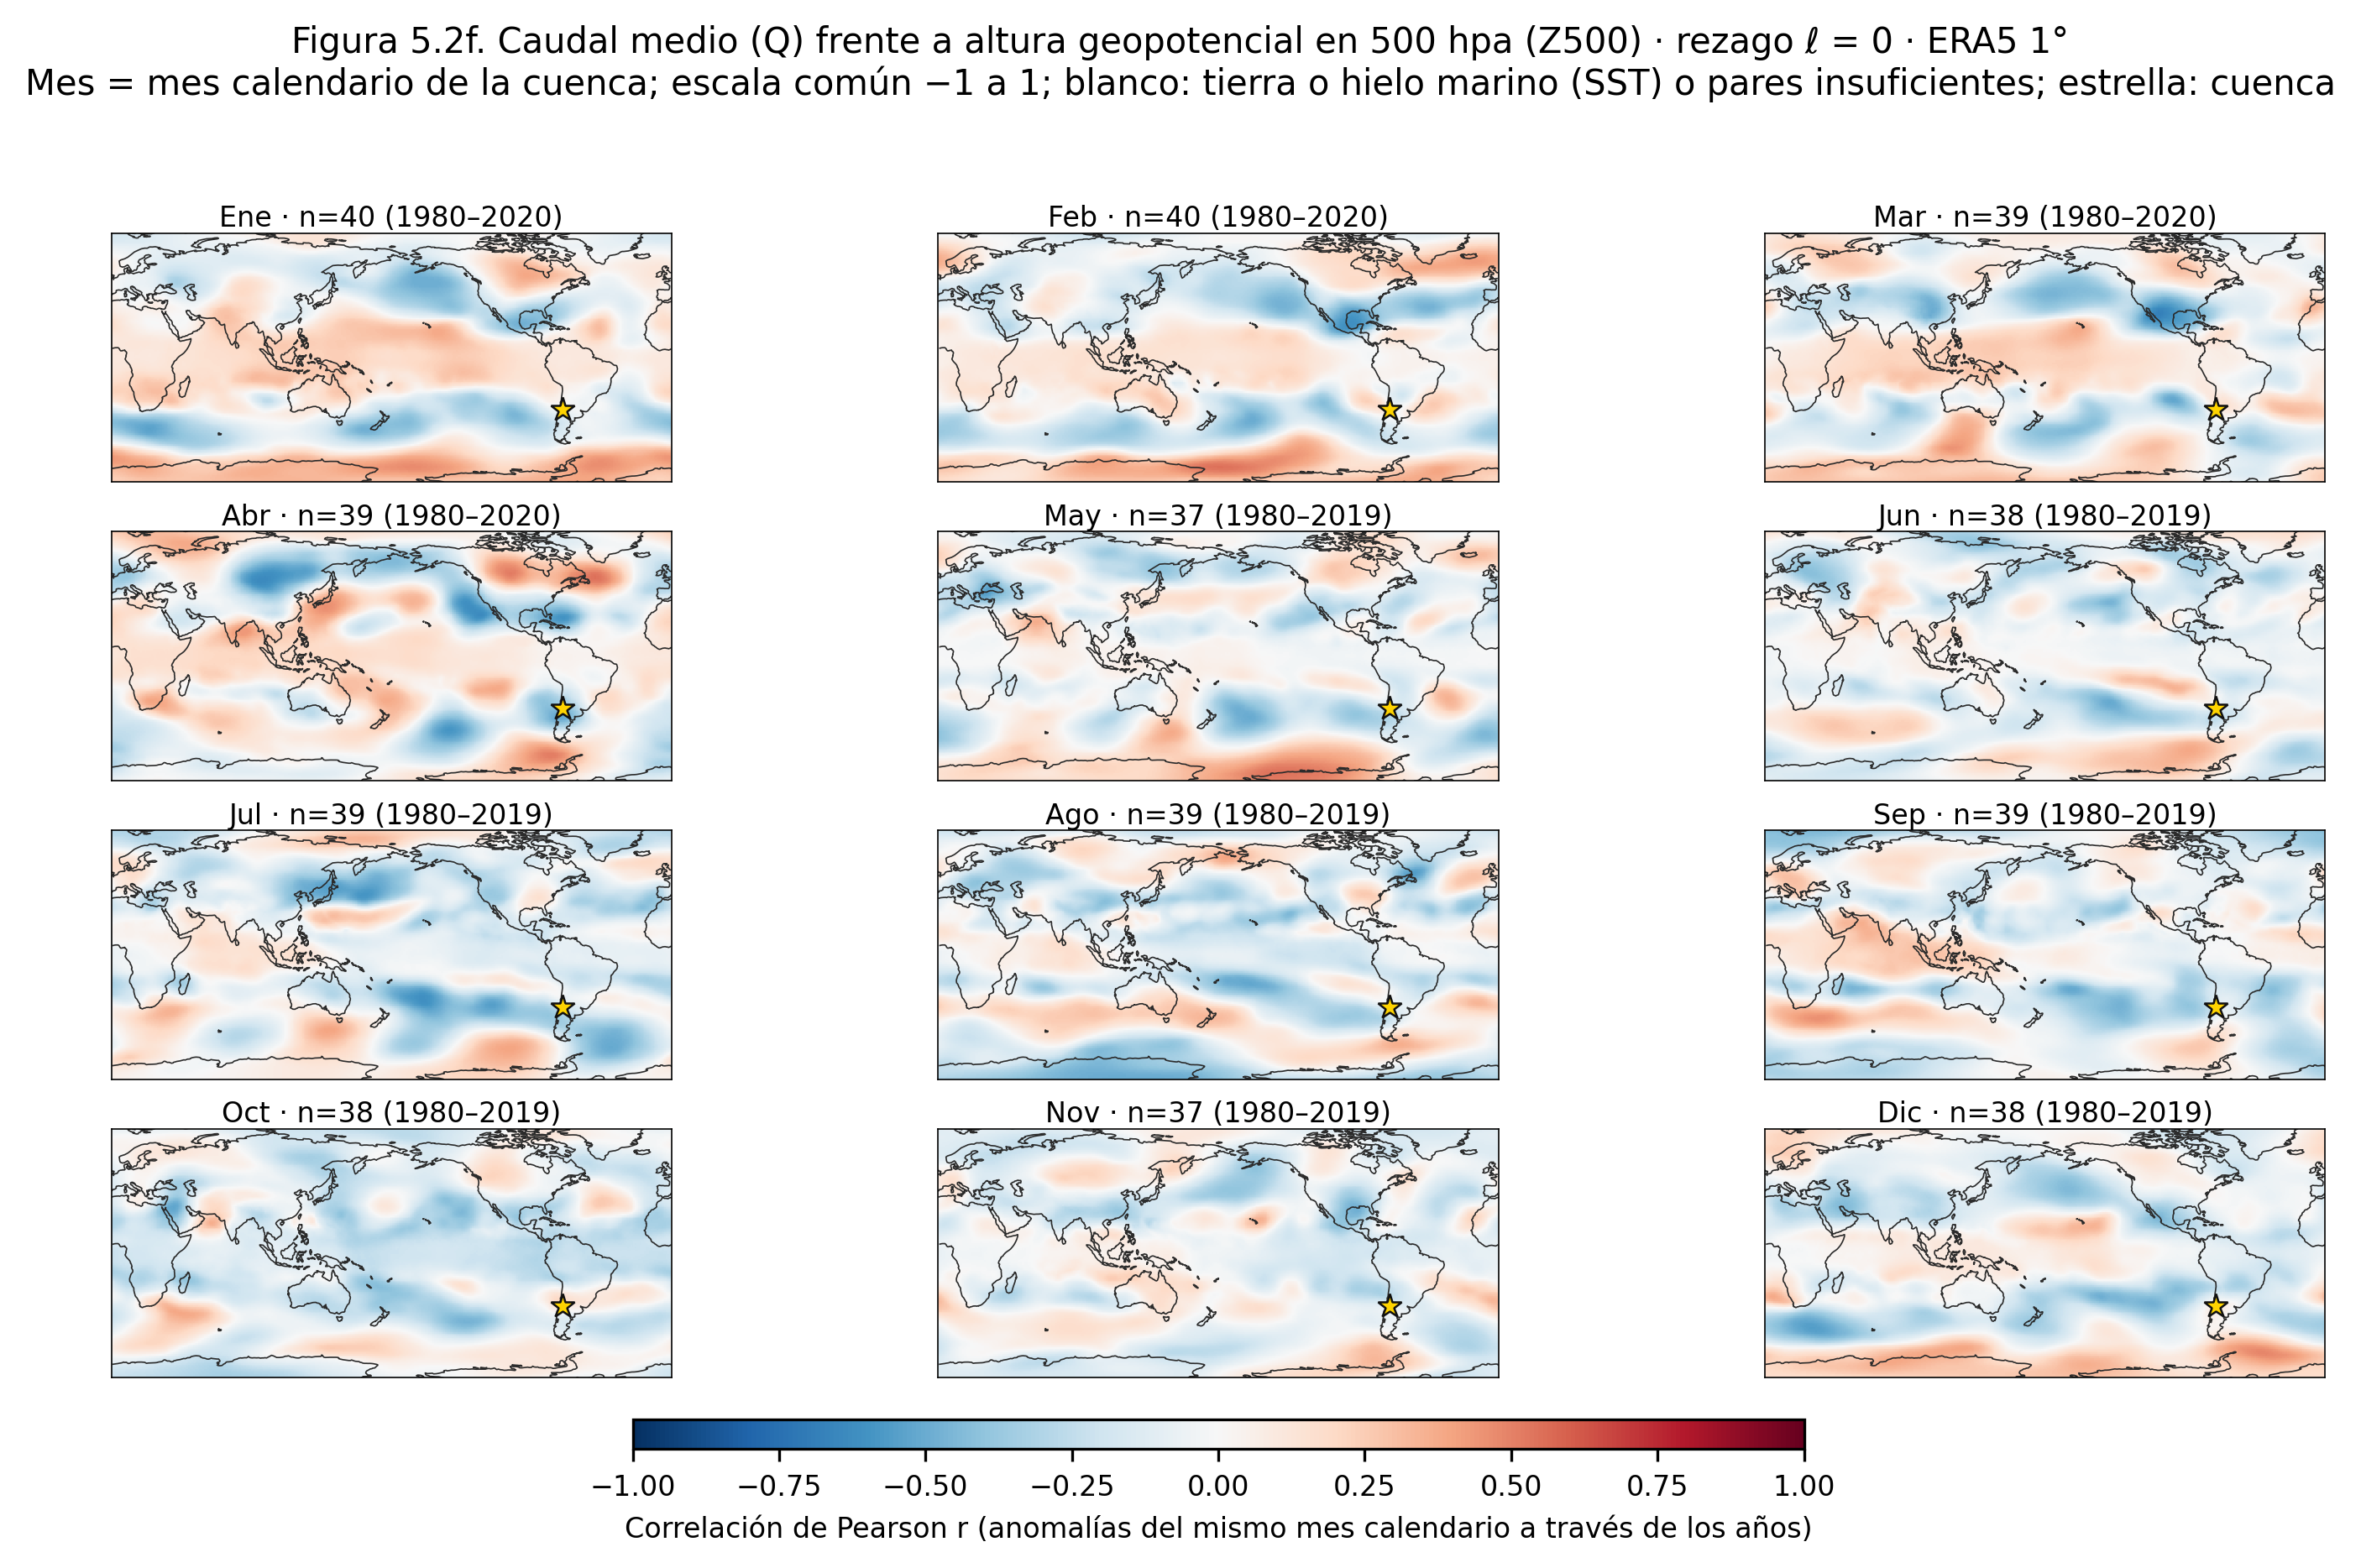
\includegraphics[width=0.88\textwidth]{figura_5_2f_q_z500.png}
\caption{$\Qm$ frente a Z500, $\ell=0$.}
\label{fig:q_z500}
\end{figure}

\begin{figure}[H]
\centering
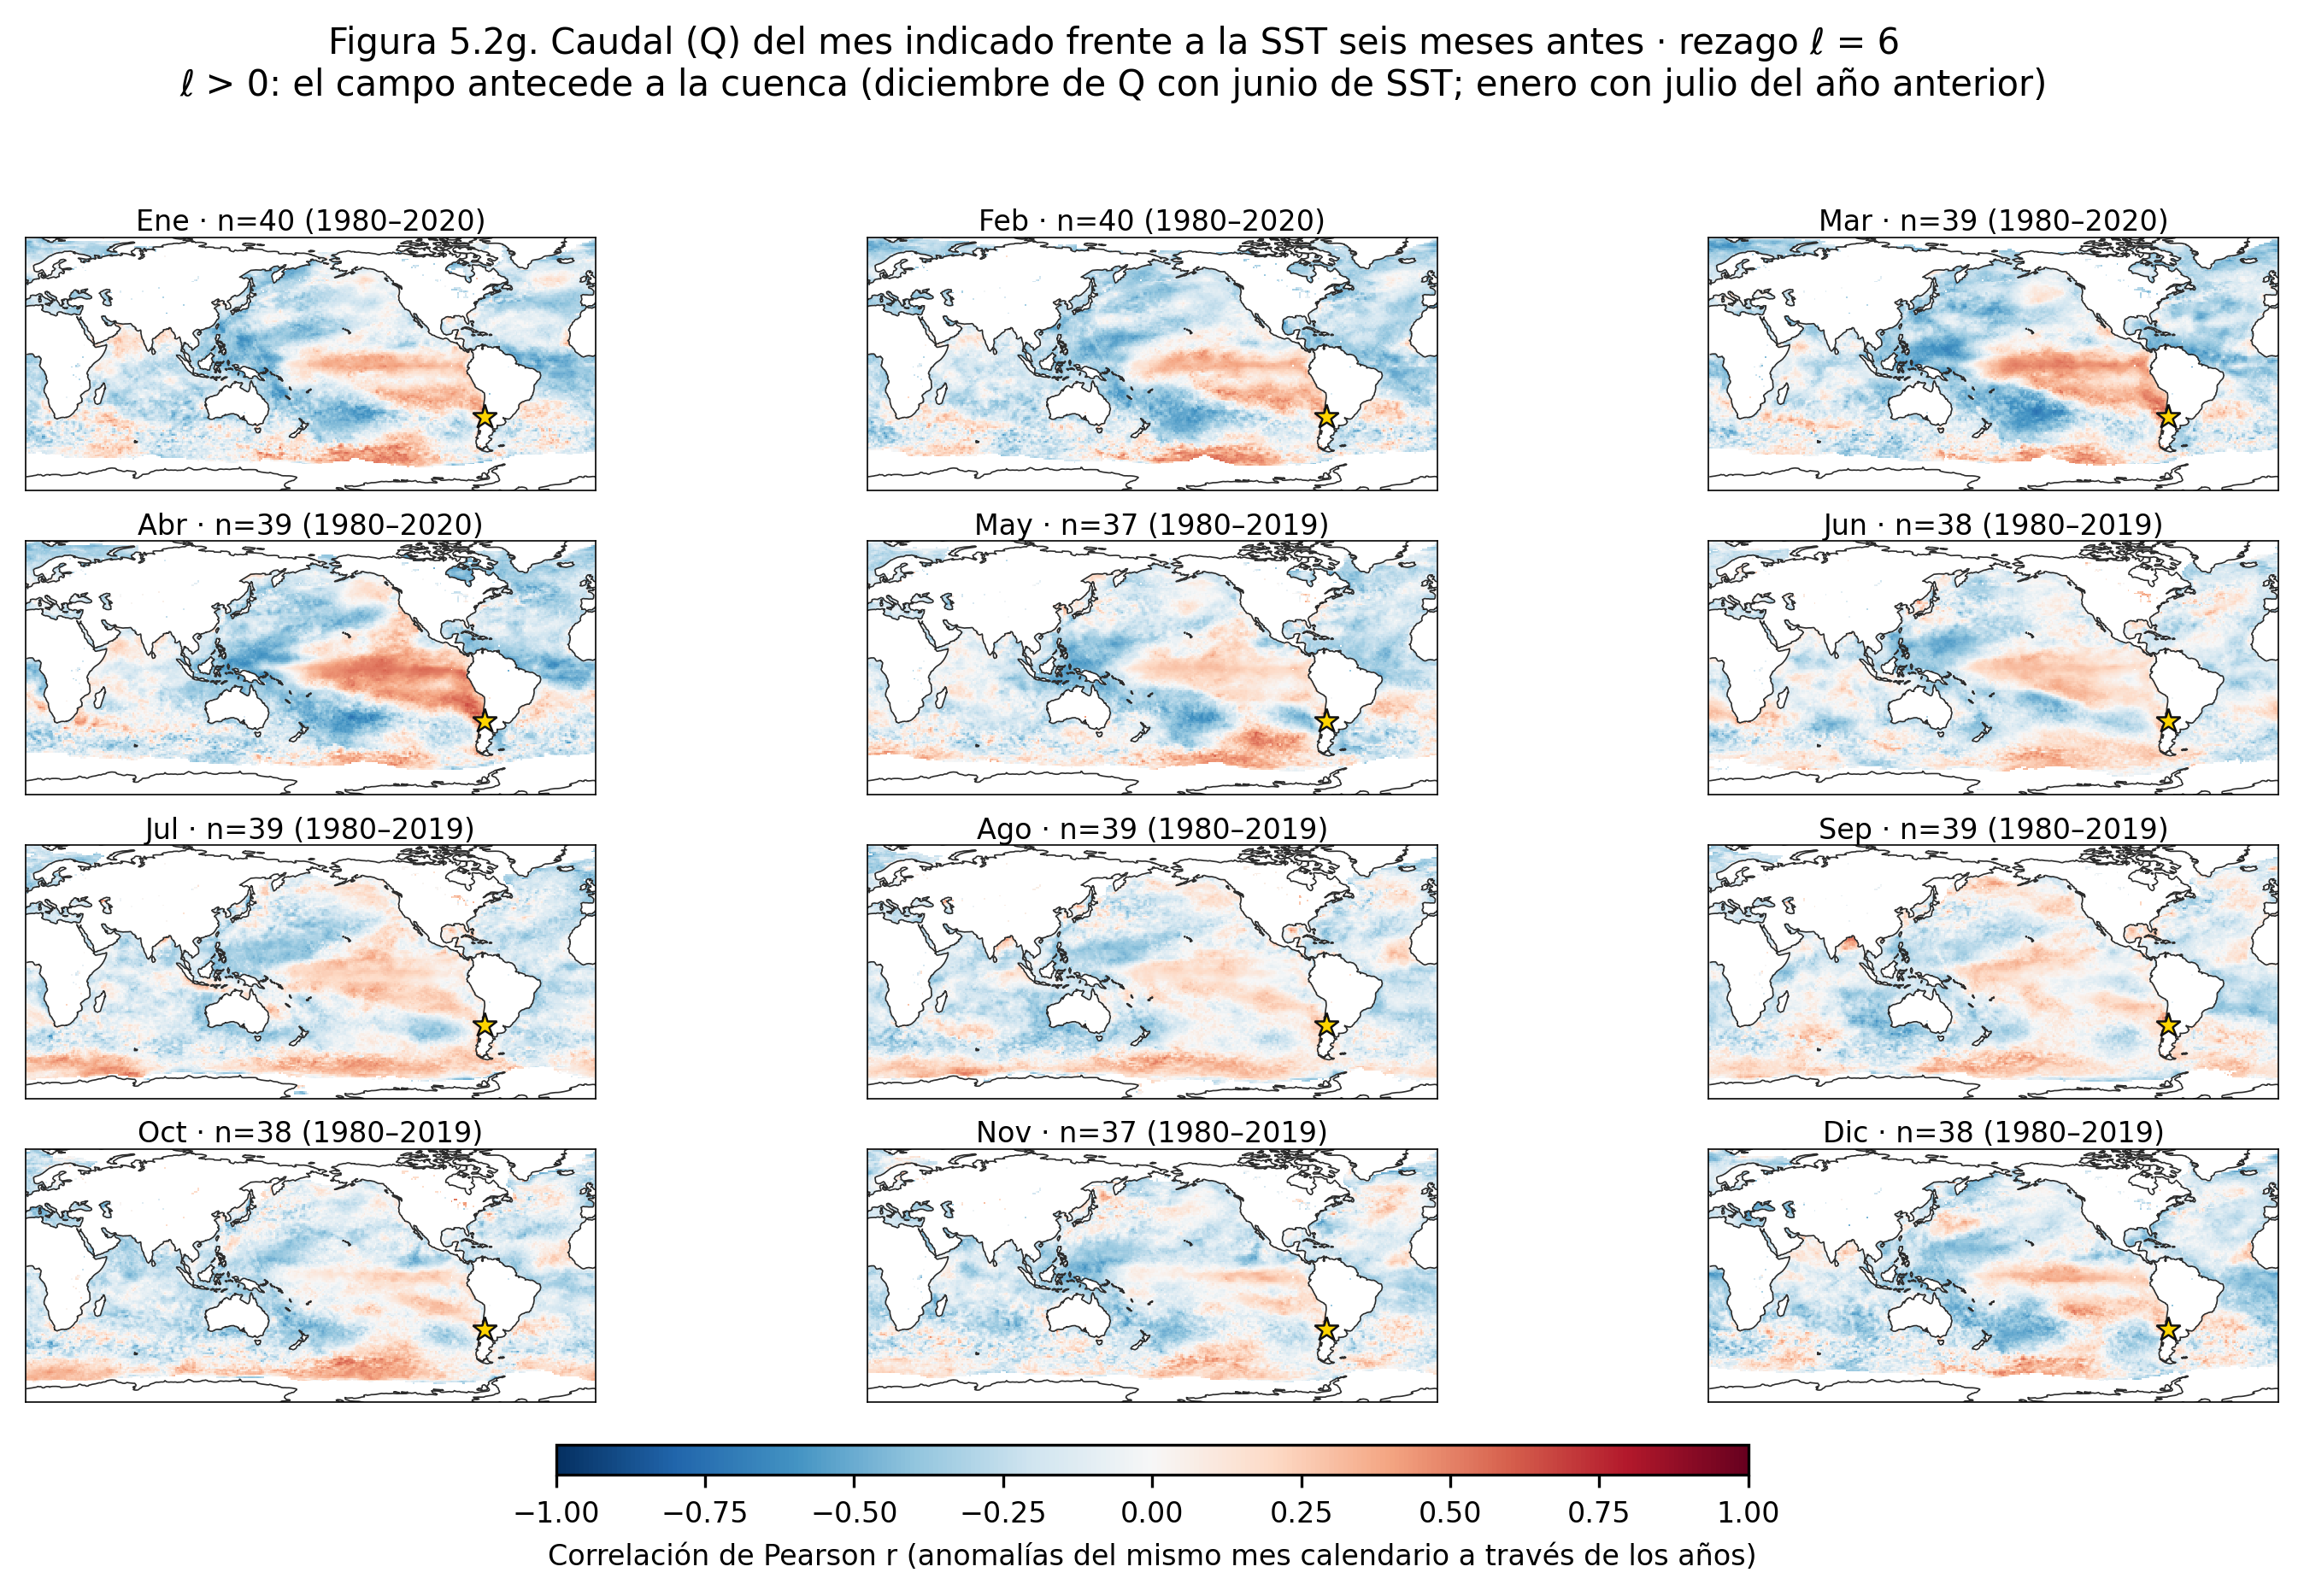
\includegraphics[width=0.88\textwidth]{figura_5_2g_q_sst_rezago6.png}
\caption{$\Qm$ frente a la SST seis meses antes ($\ell=6$).}
\label{fig:lag6}
\end{figure}

\paragraph{Pearson frente a Spearman.} Como la lluvia mensual es muy asimétrica, repetimos los mapas de SST con Spearman (Figura~\ref{fig:spear}). Los patrones casi no cambian: la correlación espacial entre los mapas de Pearson y Spearman va de 0.72 a 0.97 para $\PL$ y de 0.96 a 0.99 para $\Qm$, con diferencias medianas de 0.03 a 0.11 (\archivo{figuras/tabla_5_2_pearson_vs_spearman.csv}). Los resultados no dependen de unos pocos meses extremos. En la versión anterior del CSV, el mayo de 1993 incompleto bajaba esa correlación a 0.85 en mayo: el criterio de completitud también elimina esa sensibilidad.

\subsubsection{Robustez de los patrones (5.3)}

\paragraph{Significancia y comparaciones múltiples.} La dependencia relevante en un mapa de un mes calendario es la que hay entre años de la subserie, y resultó débil: $n_{\mathrm{eff}}$ mediano de 34--41 para $n=37$--41 (\archivo{figuras/tabla_5_3_tamano_muestra.csv}). La familia de pruebas es el conjunto de celdas de \emph{un} mapa, con FDR $\alpha=0.10$, que equivale aproximadamente a un $\alpha_{\mathrm{global}}=0.05$ en campos espacialmente correlacionados \citep{Wilks2016}. El FDR supone dependencia positiva entre pruebas, razonable para campos suaves. Aun así, 12 meses por 6 combinaciones son muchas familias, por lo que exigimos un \emph{patrón espacial coherente} y no interpretamos píxeles aislados (Figura~\ref{fig:fdr5}). La fracción de área significativa es baja para $\PL$ frente a la SST (media de 2\,\%, máxima de 15\,\% en octubre) y mayor para $\PL$ frente a la PNM (máxima de 15\,\%) y para $\Qm$ frente a la SST (media de 10\,\%, máxima de 23\,\%). Con 40 años, una correlación de 0.4 apenas supera el umbral local, de modo que la ausencia de punteado no implica ausencia de asociación. Con las anomalías de todos los meses juntas ($n\approx480$; Figura~\ref{fig:todos}) emergen tres patrones claros: la ``herradura'' de ENSO en la SST para $\Qm$; un patrón de tipo Oscilación del Sur en la PNM para $\Qm$; y, para $\PL$, un dipolo de PNM con un centro negativo frente a Chile central y otro positivo sobre los mares de Amundsen y Bellingshausen.

\begin{figure}[H]
\centering
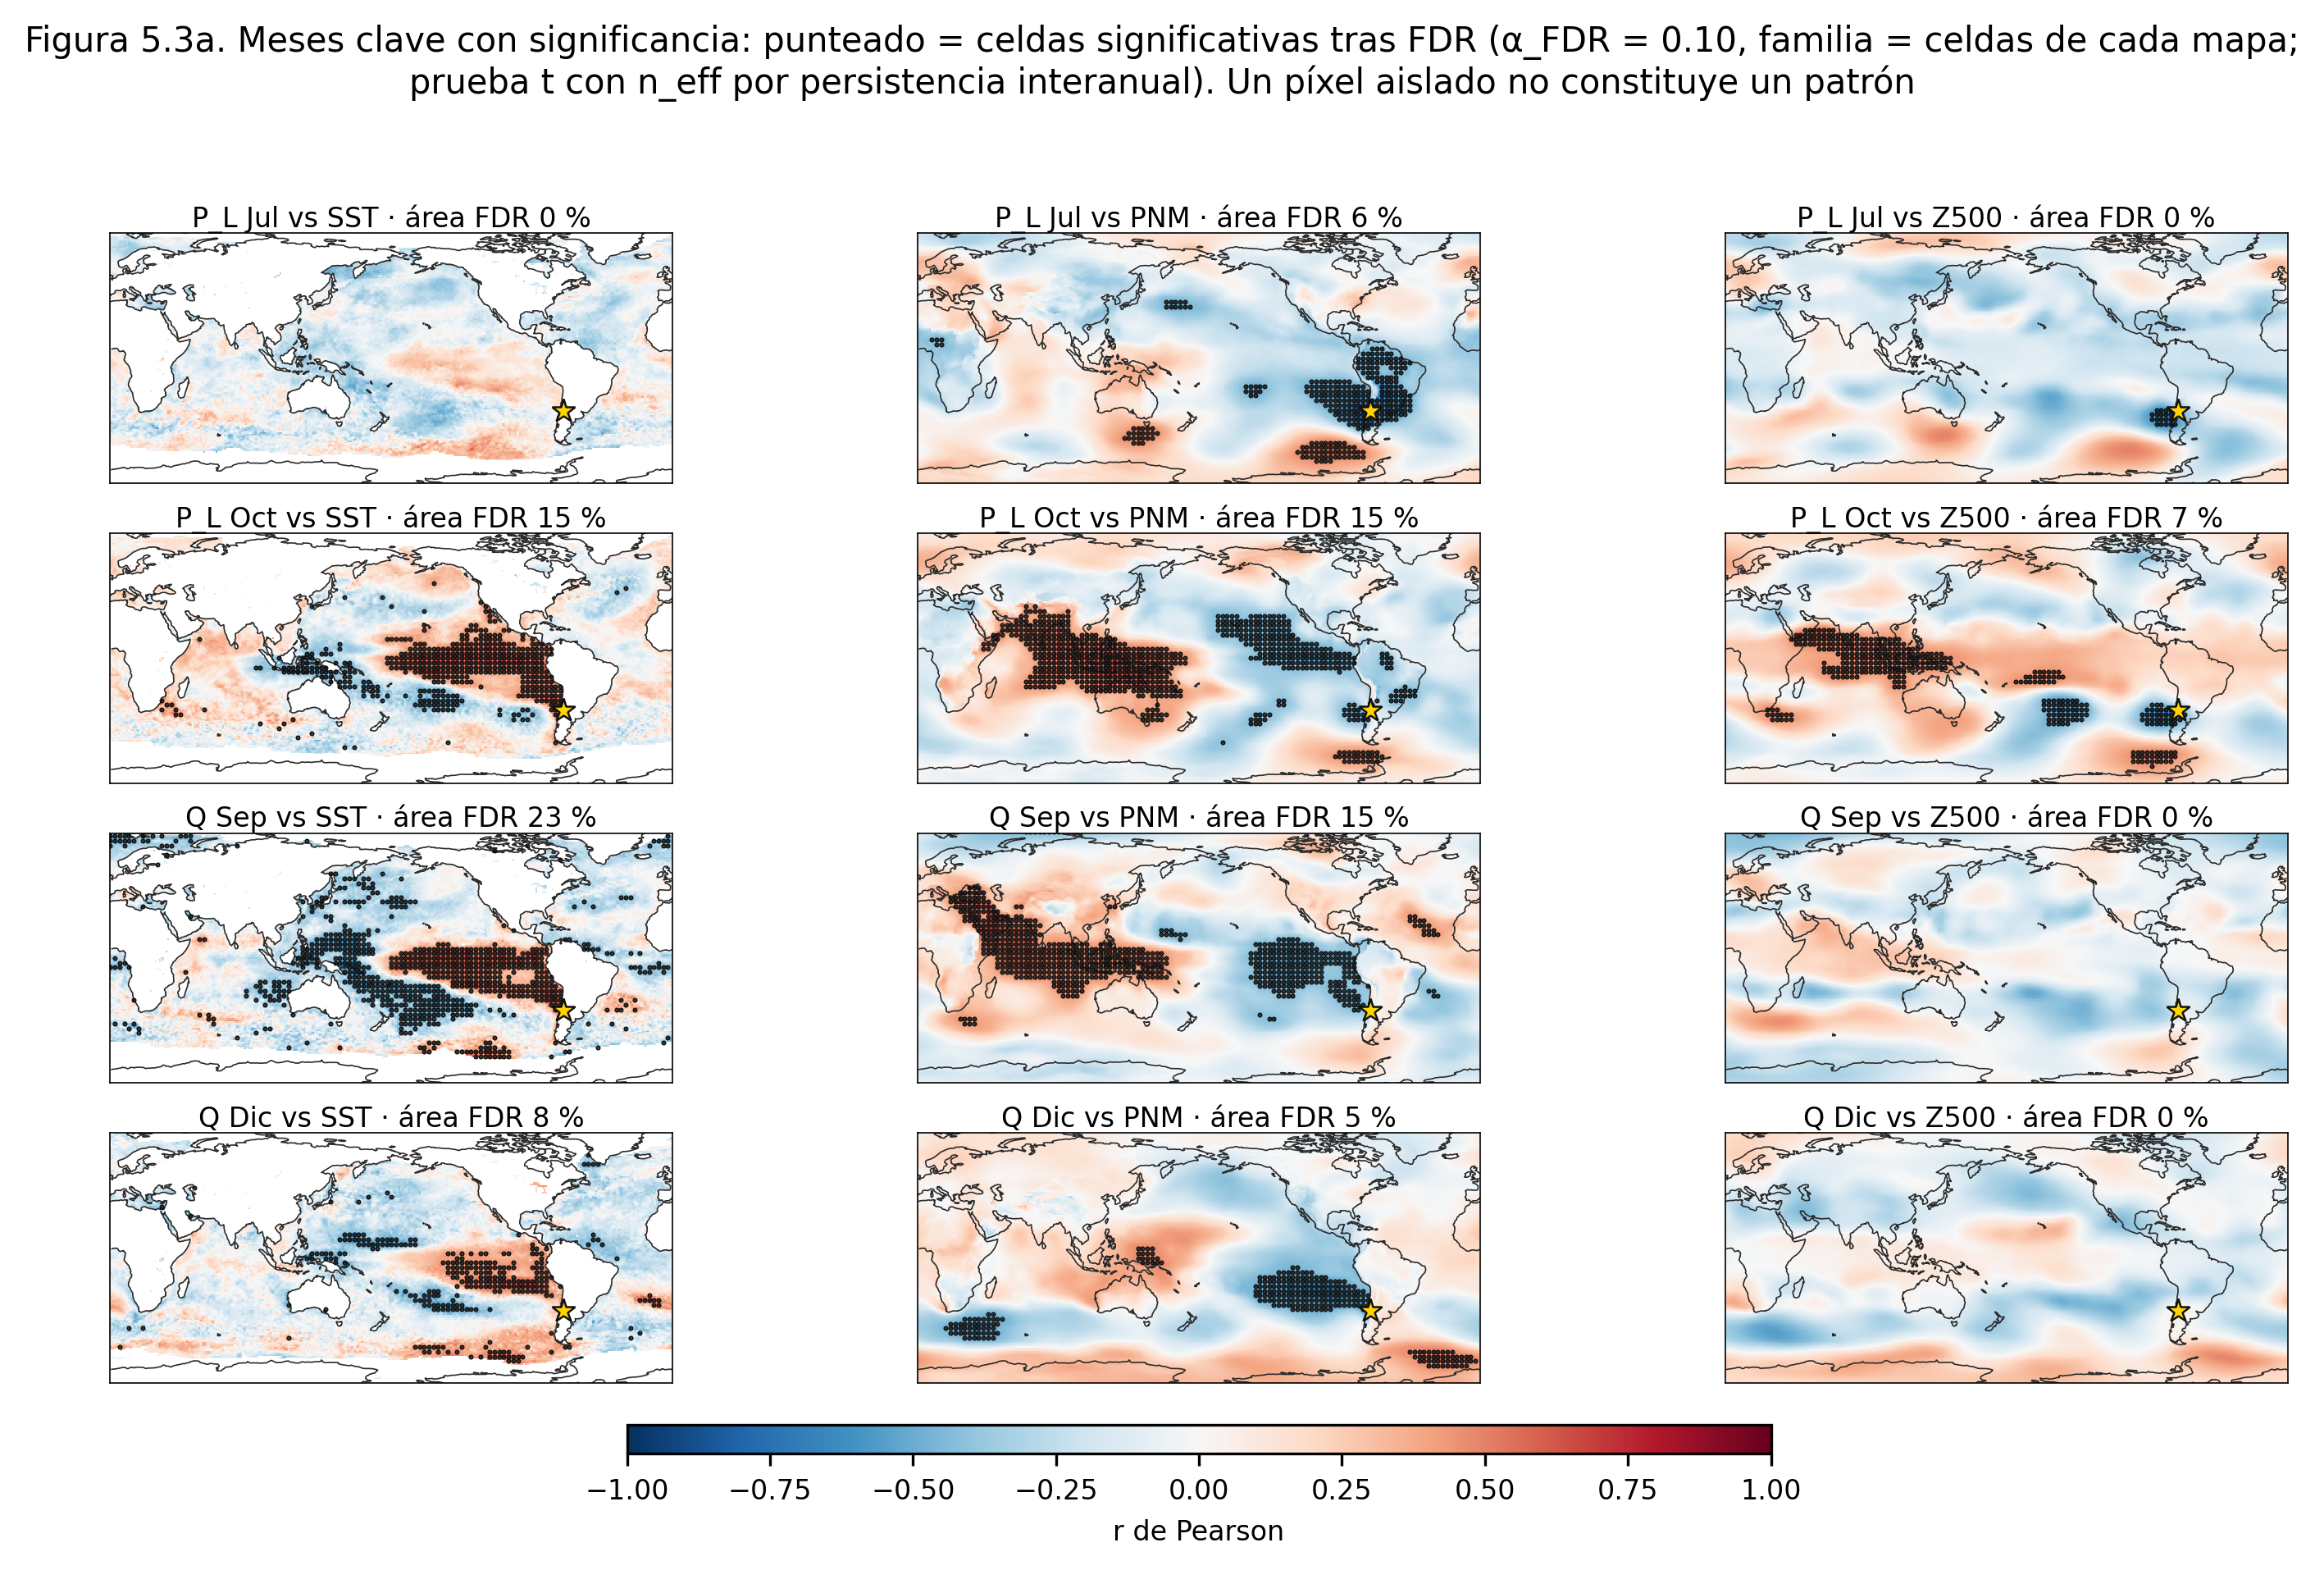
\includegraphics[width=0.85\textwidth]{figura_5_3a_significancia_fdr.png}
\caption{Meses clave con punteado de las celdas significativas tras FDR. Script \archivo{18_p5_3_robustez.py}.}
\label{fig:fdr5}
\end{figure}

\begin{figure}[H]
\centering
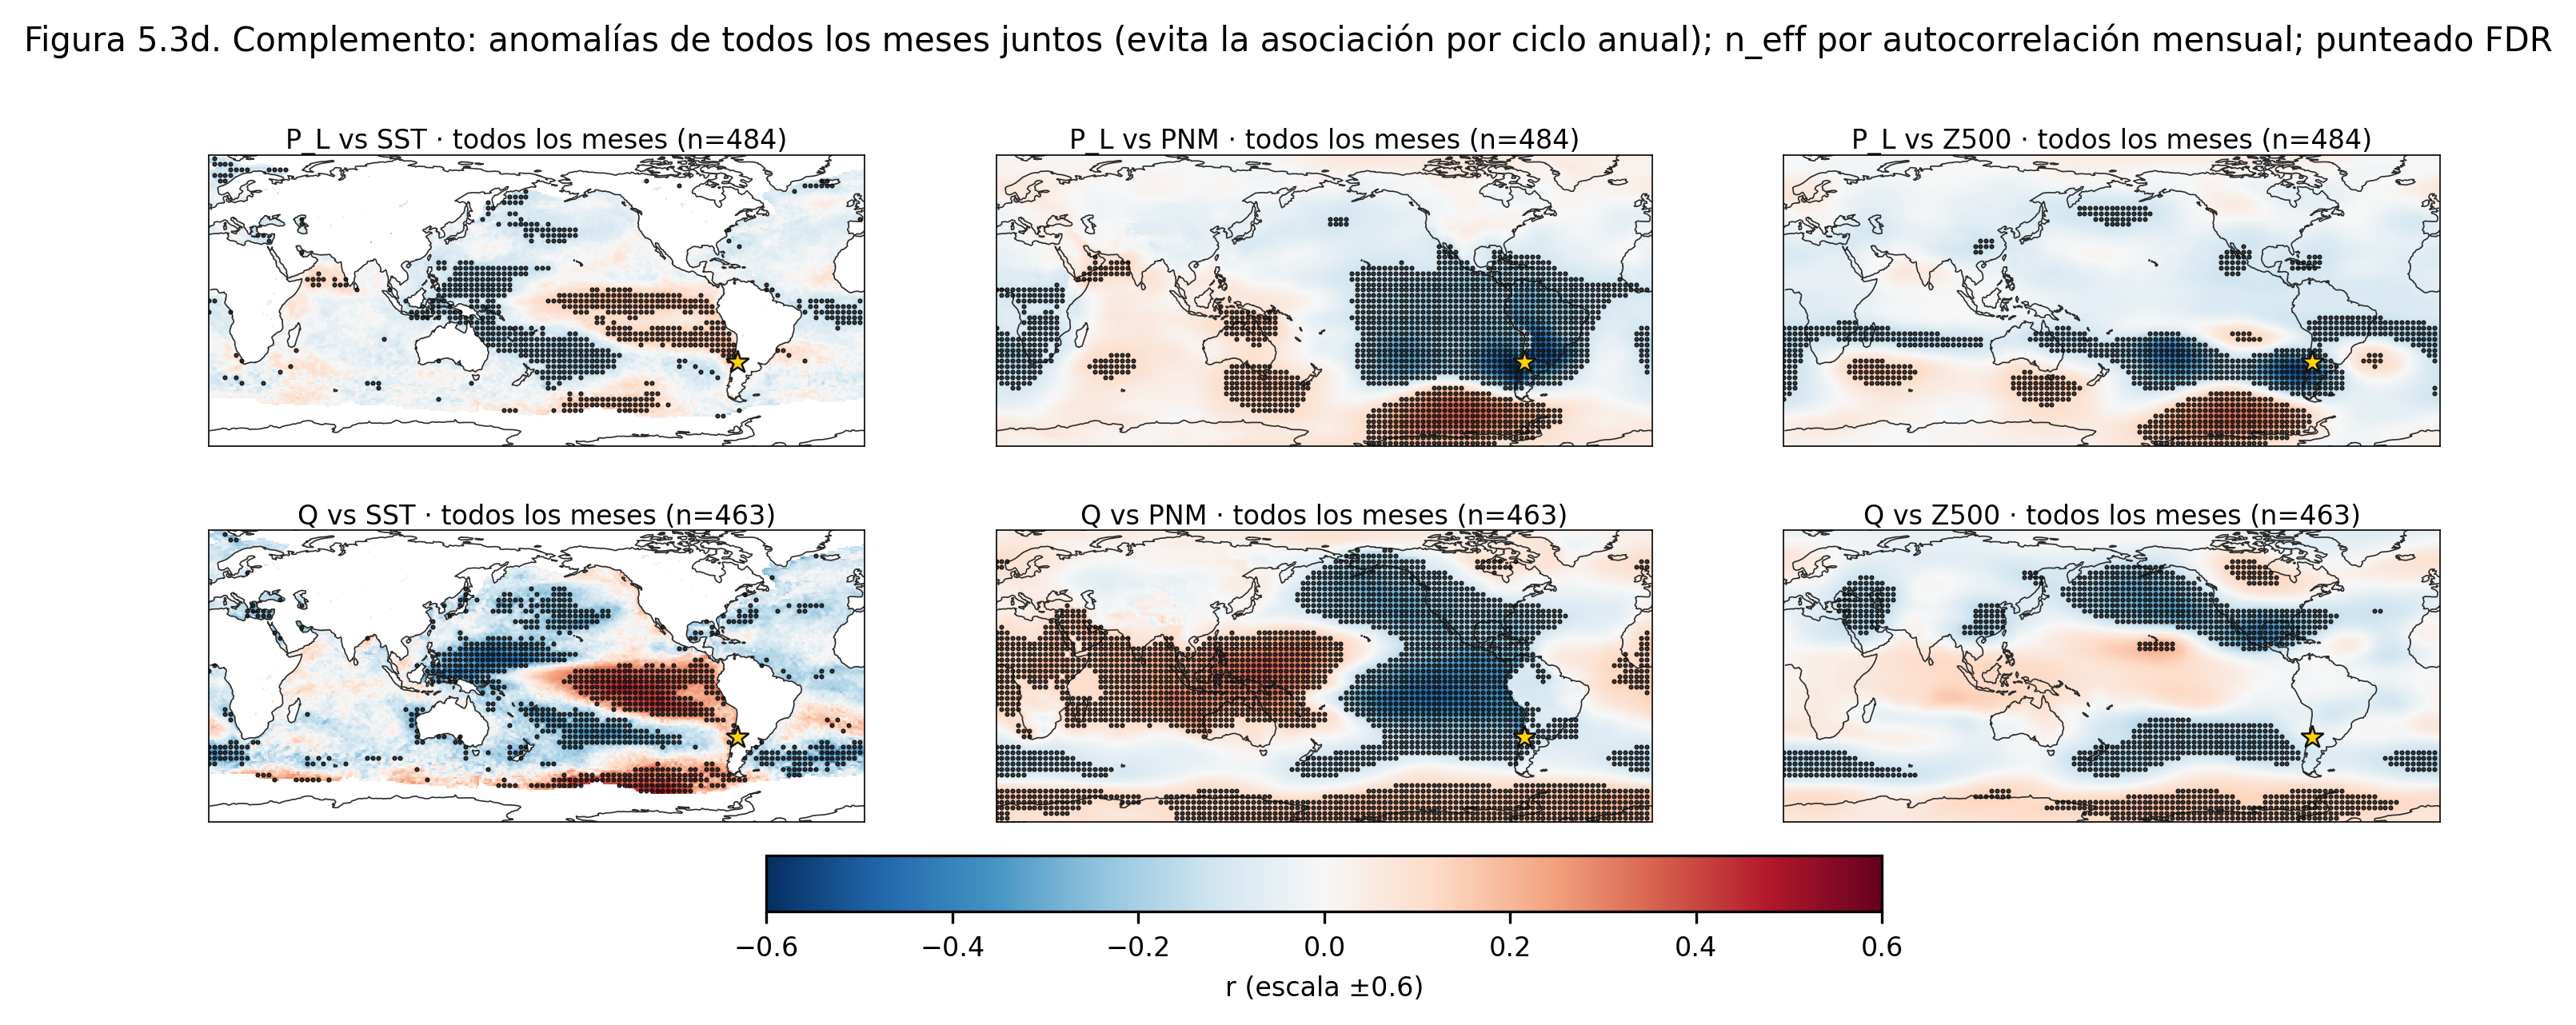
\includegraphics[width=0.92\textwidth]{figura_5_3d_todos_los_meses.png}
\caption{Correlación con las anomalías de todos los meses juntos (sin ciclo anual compartido), con punteado FDR.}
\label{fig:todos}
\end{figure}

\paragraph{Tendencias, extremos, fuente y subperiodos.} Comparamos los patrones mediante su correlación espacial en el Pacífico (60$^\circ$S--60$^\circ$N, 120$^\circ$E--60$^\circ$W; \archivo{figuras/tabla_5_3_robustez.csv}):
\begin{itemize}
\item \textbf{Sin tendencia} (retirada en ambas series, por mes y celda; Figura~\ref{fig:tend5}): mediana de 0.88--0.99. Para $\Qm$, la asociación con Niño 3.4 incluso aumenta (enero: de 0.45 a 0.50). La tendencia del caudal no produce estas correlaciones: enmascara parte de la asociación interanual.
\item \textbf{Sin los tres años de mayor anomalía} de cada mes: mediana de 0.74--0.92.
\item \textbf{IMERG frente a $\PL$}, con los mismos meses de 2000--2020: mediana de 0.82--0.86, salvo en los meses secos de verano. La conclusión no depende de la fuente de precipitación.
\item \textbf{Subperiodos} 1980--1999 frente a 2000--2019 (Figura~\ref{fig:estab5}): en toda la cuenca del Pacífico los patrones \emph{no} se reproducen (mediana de 0.04--0.35). Con 20 años por mapa el ruido muestral es grande, y además hay no estacionariedad real (Sección~\ref{sec:p54}).
\end{itemize}

\begin{figure}[H]
\centering
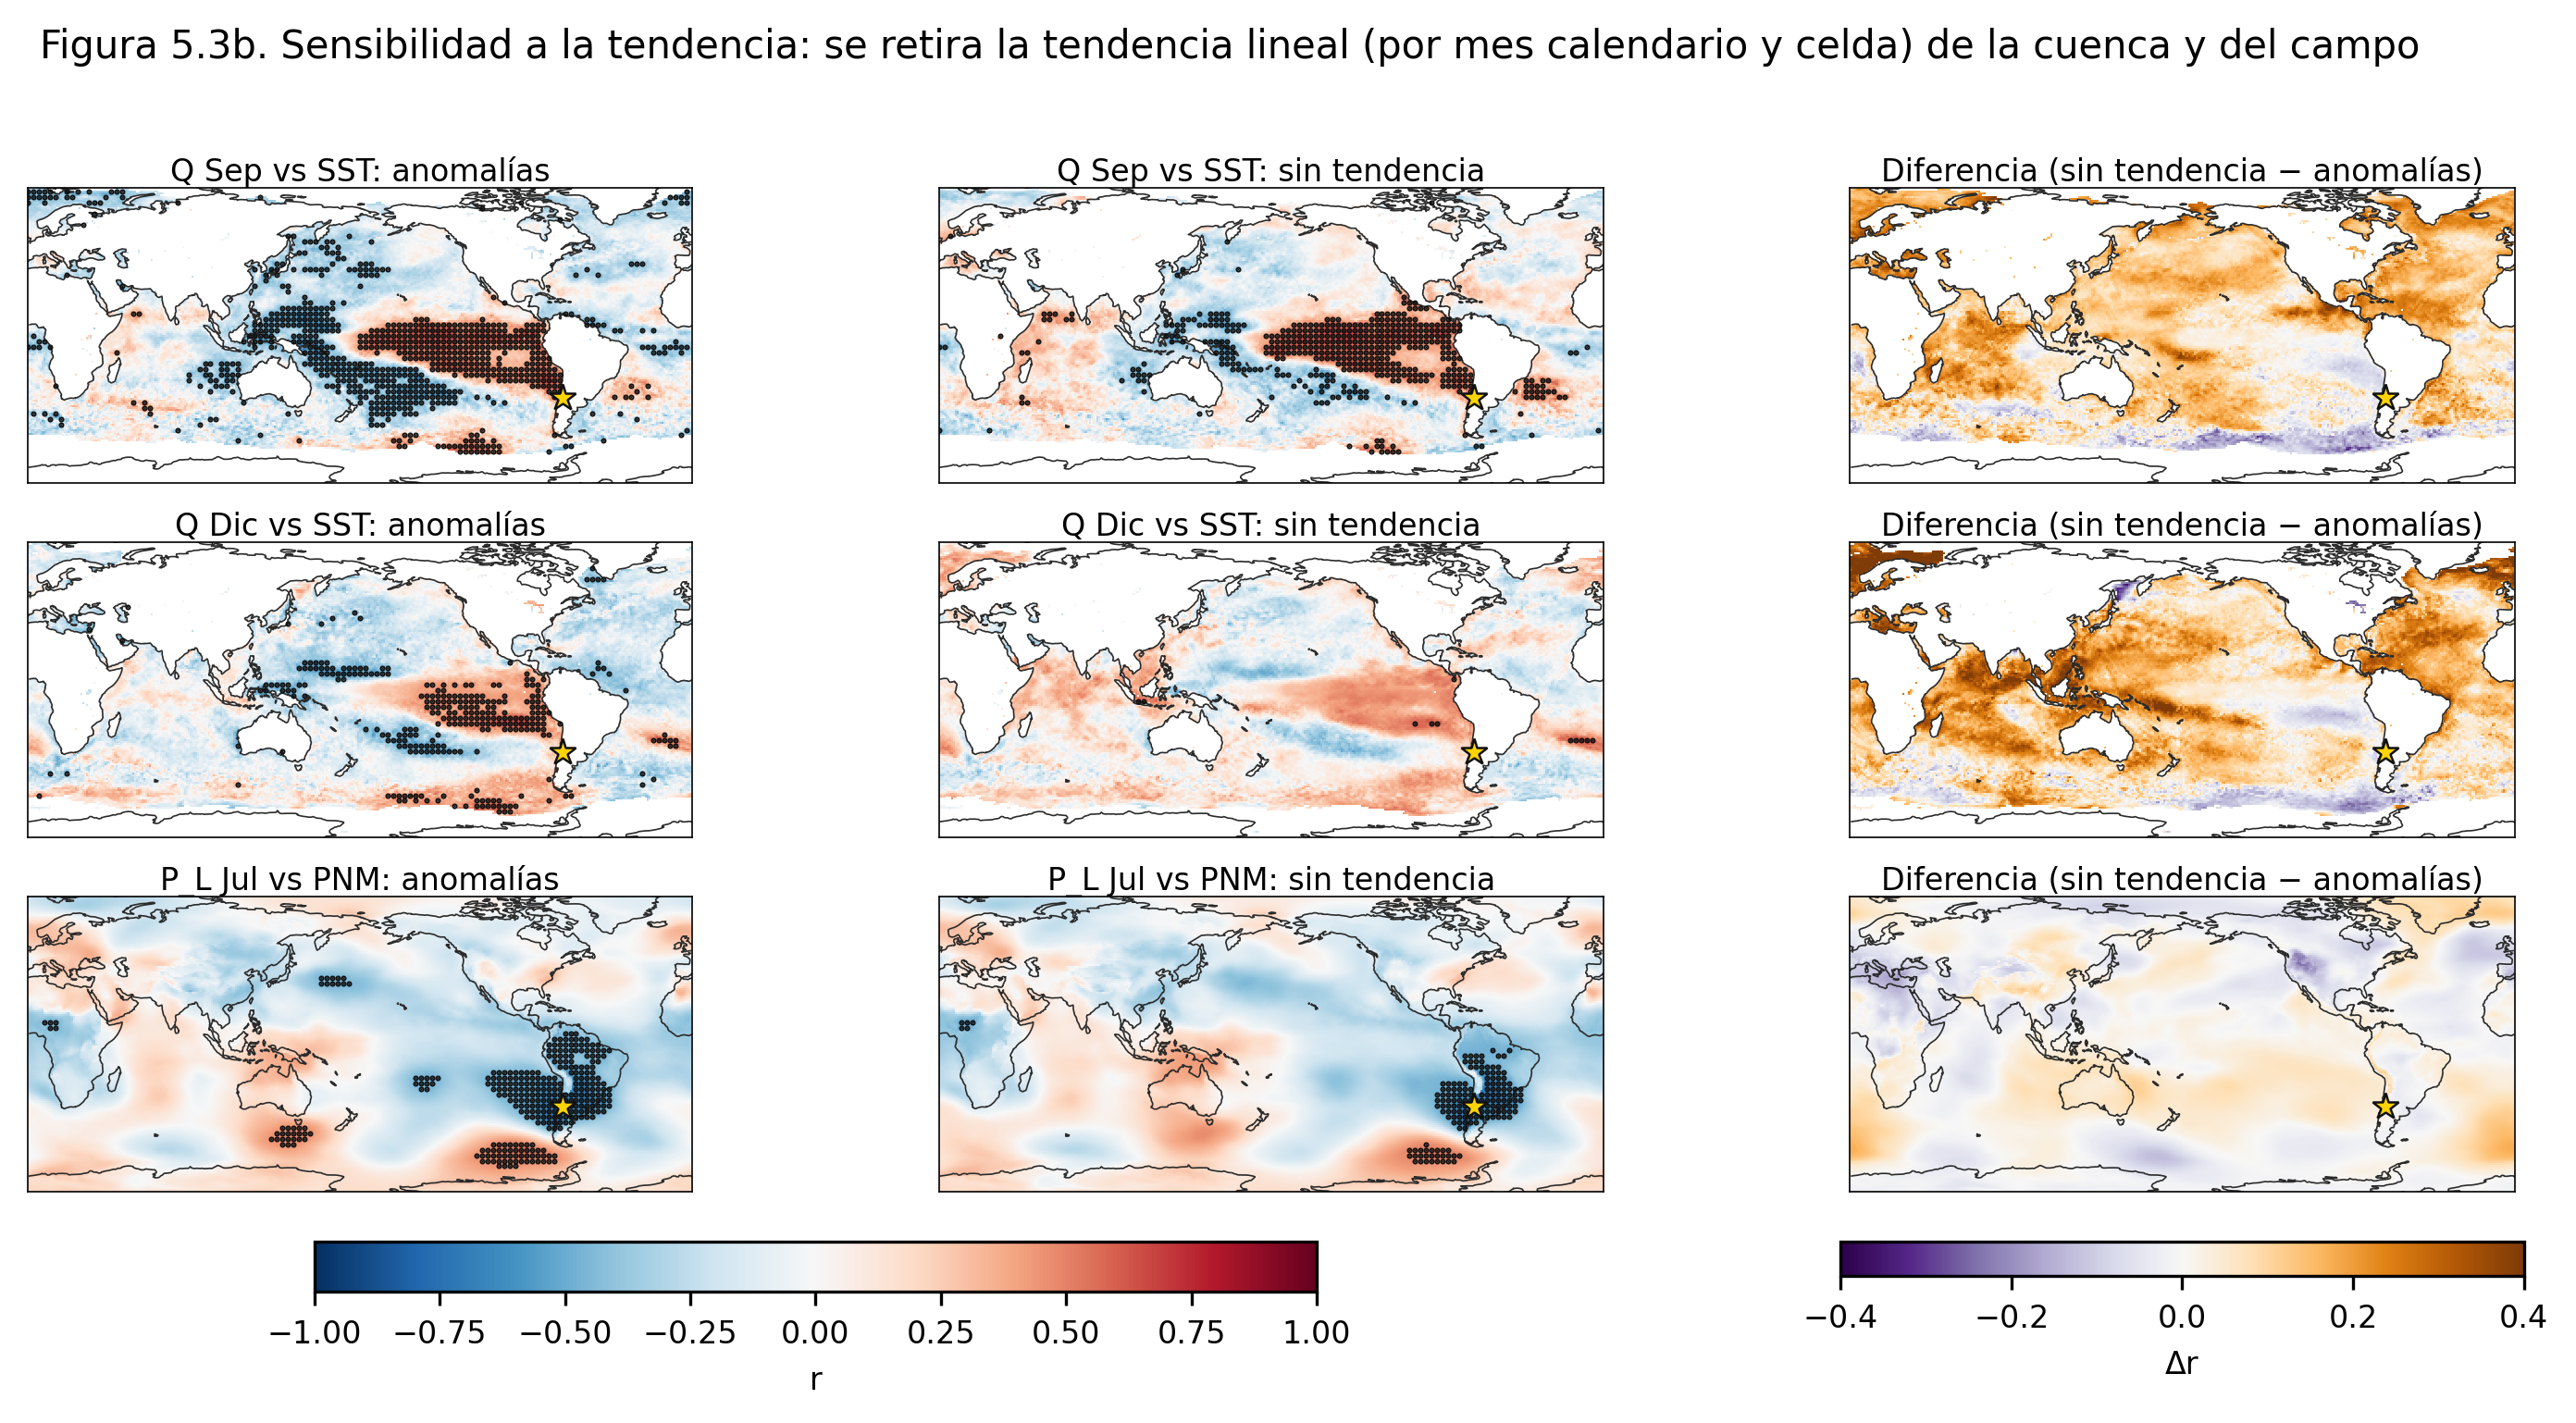
\includegraphics[width=0.85\textwidth]{figura_5_3b_tendencia.png}
\caption{Correlación con anomalías, sin tendencia y su diferencia, para $\Qm$ en septiembre y diciembre frente a la SST y $\PL$ en julio frente a la PNM.}
\label{fig:tend5}
\end{figure}

\paragraph{Producto de SST: ERA5 frente a ERSST v5.}
\label{sec:ersst}
ERSST v5 es una reconstrucción mensual a 2$^\circ$ basada en observaciones in situ \citep{Huang2017}, independiente del sistema de asimilación de ERA5. \archivo{scripts/24_p5_3_contraste_ersst.py} la descarga de NOAA PSL, guarda el subconjunto usado (\archivo{datos/campos_ersst/}) y repite con la misma referencia, años y funciones los cálculos que dependen de la SST (Figura~\ref{fig:ersst}). El índice Niño 3.4 de ambos productos correlaciona $r=0.983$ (diferencia cuadrática media de 0.16~$^\circ$C), y los perfiles mensuales de $\PL$ y $\Qm$ con Niño 3.4 cambian como máximo 0.08 en $r$. La correlación de patrón en el Pacífico entre los mapas de ERA5 (remuestreados a 2$^\circ$) y los de ERSST es de 0.85 a 0.93 para $\Qm$ y de 0.65 a 0.94 para $\PL$, con los valores bajos en los meses secos de verano, cuando la asociación es débil en ambos productos (\archivo{figuras/tabla_5_5_contraste_ersst_patrones.csv}). Las conclusiones del punto 5 sobre la SST no dependen del producto.

\begin{figure}[H]
\centering
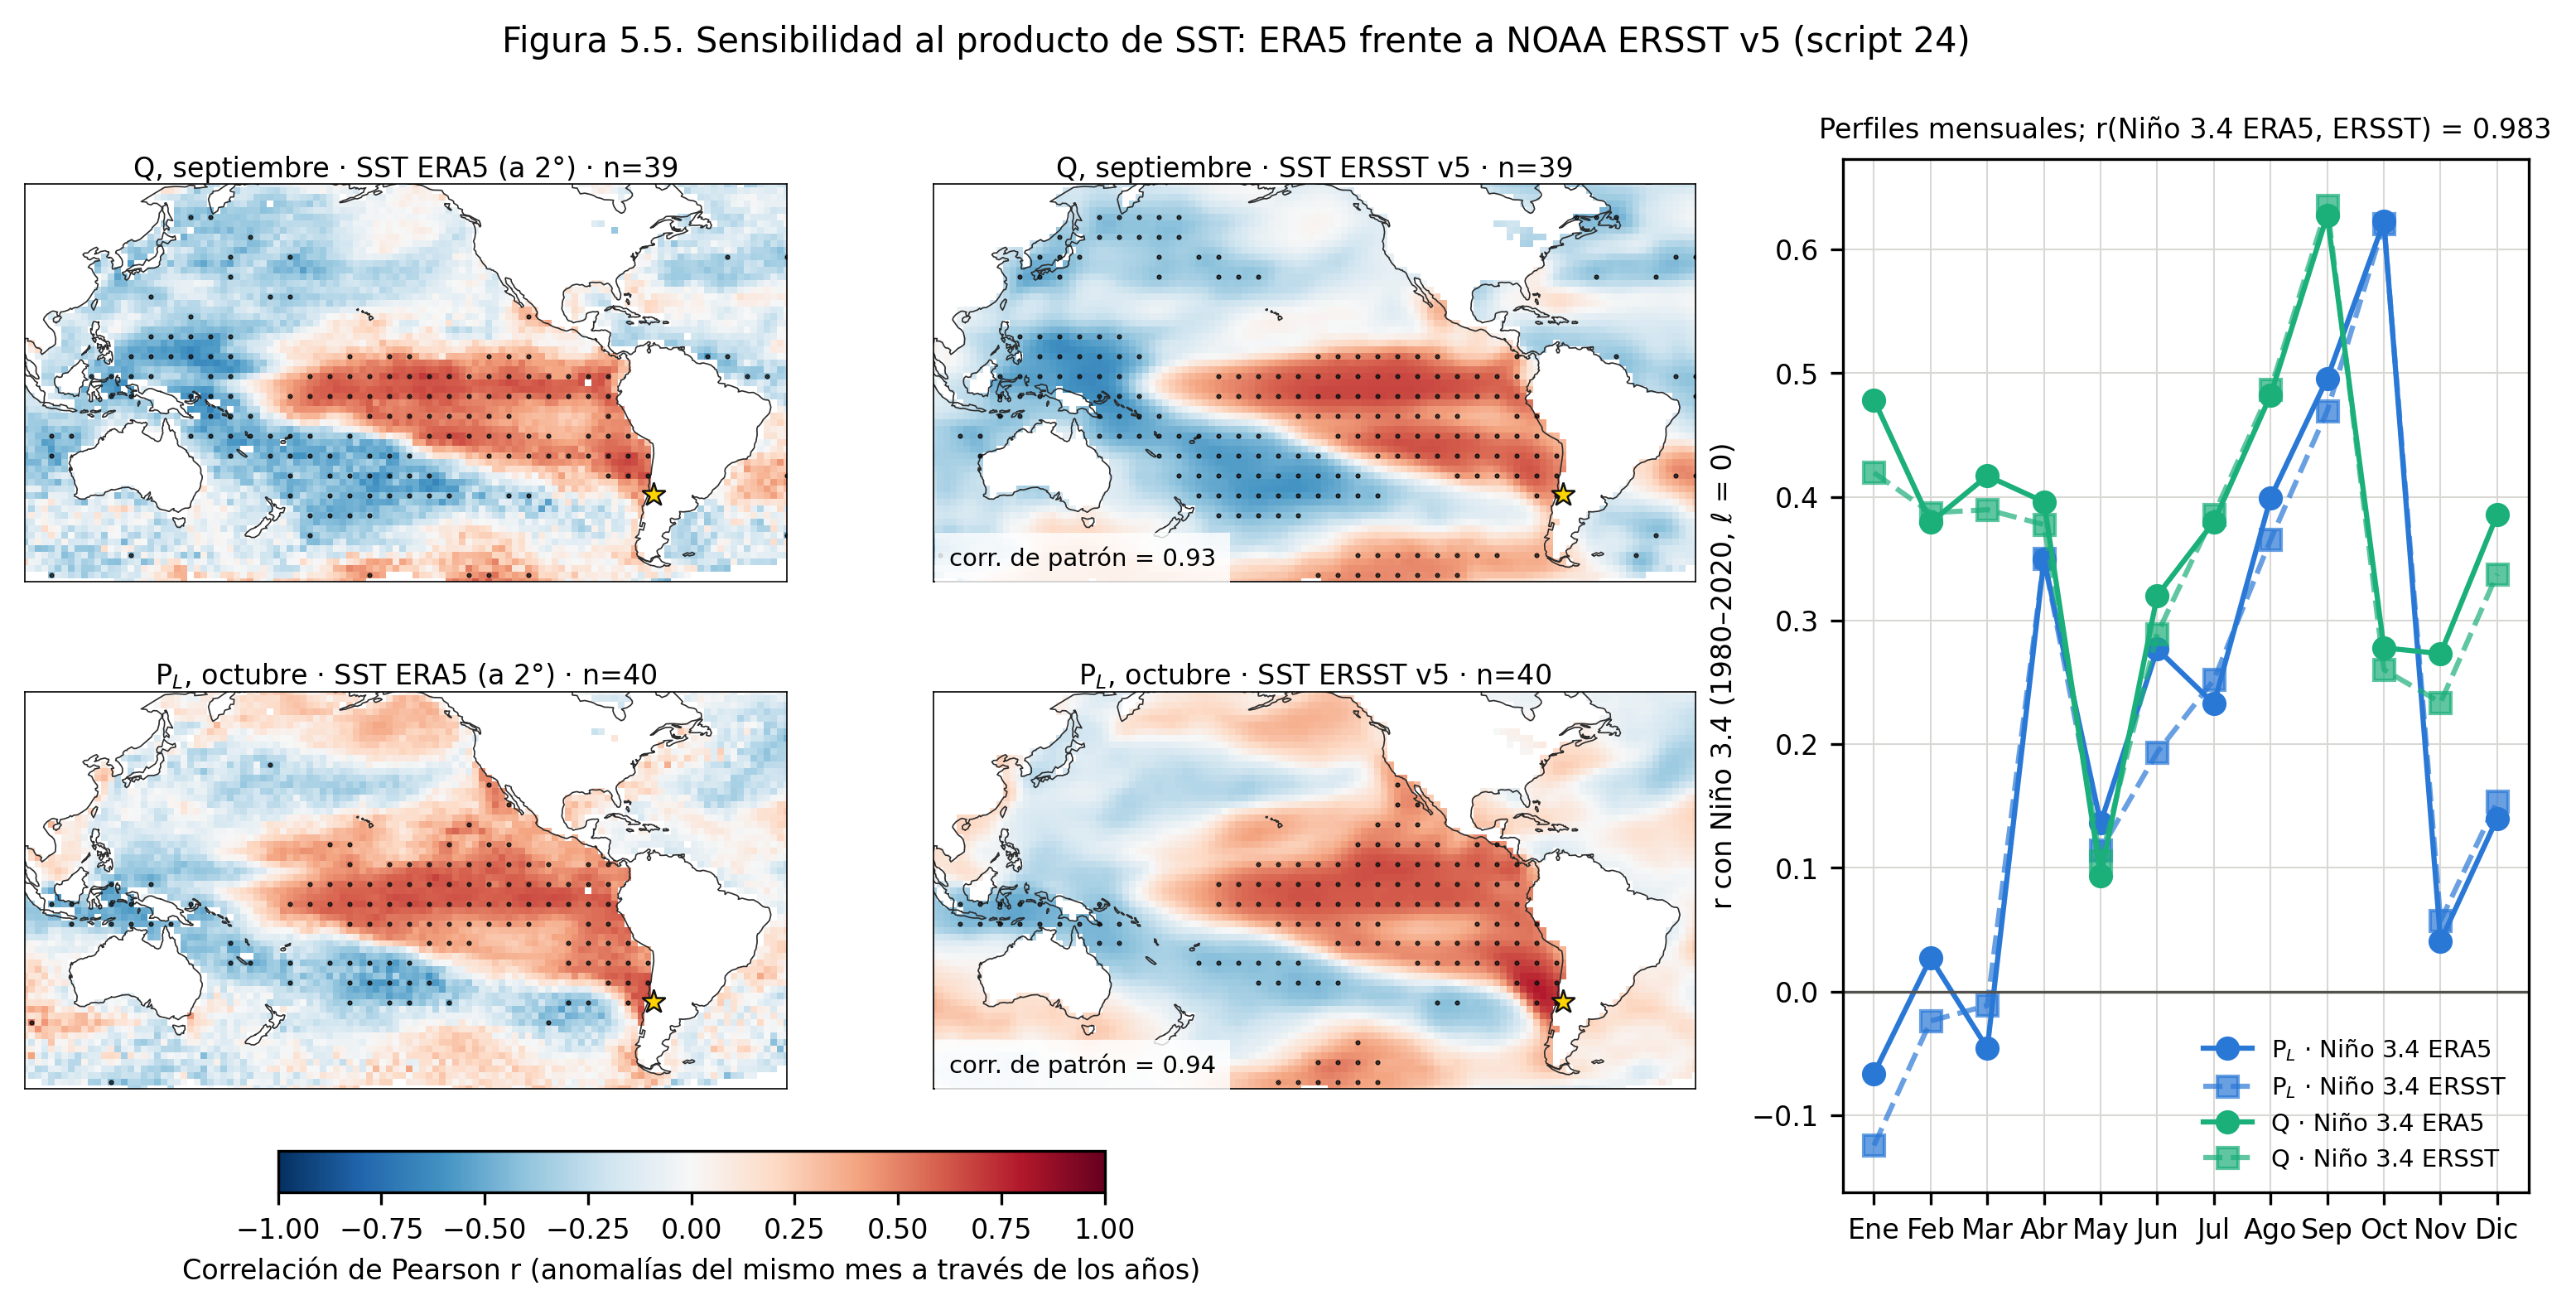
\includegraphics[width=\textwidth]{figura_5_5_contraste_ersst.png}
\caption{Sensibilidad al producto de SST: mapas de correlación de $\Qm$ (septiembre) y $\PL$ (octubre) con ERA5 remuestreado a 2$^\circ$ y con ERSST v5, y perfiles mensuales frente a Niño 3.4 con ambos productos. Script \archivo{24_p5_3_contraste_ersst.py}.}
\label{fig:ersst}
\end{figure}

\subsubsection{Interpretación física e integración (5.4)}
\label{sec:p54}

Para no elegir regiones a partir de los propios mapas, definimos tres índices \emph{a priori} según el mecanismo: Niño 3.4, PNM del Pacífico sureste y Z500 sobre Chile central (Sección~\ref{sec:metodologia}). La Tabla~\ref{tab:indices} y la Figura~\ref{fig:perfiles} resumen sus correlaciones mes a mes.

\begin{table}[H]
\centering\footnotesize\setlength{\tabcolsep}{3.4pt}
\caption{Correlación (1980--2020, $\ell=0$) de $\PL$ y $\Qm$ con los tres índices (\archivo{figuras/tabla_5_4_perfiles_indices.csv}). En negrita: $q_{\mathrm{FDR}}<0.05$ en la familia de 72 pruebas.}
\label{tab:indices}
\begin{tabular}{llrrrrrrrrrrrr}
\toprule
 & Índice & Ene & Feb & Mar & Abr & May & Jun & Jul & Ago & Sep & Oct & Nov & Dic \\
\midrule
$\PL$ & Niño 3.4 & $-$0.07 & 0.03 & $-$0.05 & 0.35 & 0.14 & 0.28 & 0.23 & \textbf{0.40} & \textbf{0.50} & \textbf{0.62} & 0.04 & 0.14 \\
  & PNM SE & 0.04 & $-$0.06 & 0.01 & \textbf{$-$0.38} & \textbf{$-$0.64} & \textbf{$-$0.47} & \textbf{$-$0.63} & \textbf{$-$0.63} & \textbf{$-$0.56} & \textbf{$-$0.46} & $-$0.19 & $-$0.32 \\
  & Z500 Chile & 0.05 & $-$0.34 & \textbf{$-$0.37} & \textbf{$-$0.64} & \textbf{$-$0.65} & \textbf{$-$0.58} & \textbf{$-$0.69} & \textbf{$-$0.46} & \textbf{$-$0.47} & \textbf{$-$0.68} & $-$0.33 & \textbf{$-$0.50} \\
\midrule
 $\Qm$ & Niño 3.4 & \textbf{0.48} & \textbf{0.38} & \textbf{0.42} & \textbf{0.40} & 0.09 & 0.32 & \textbf{0.38} & \textbf{0.48} & \textbf{0.63} & 0.28 & 0.27 & \textbf{0.39} \\
  & PNM SE & \textbf{$-$0.41} & $-$0.19 & $-$0.33 & $-$0.30 & $-$0.35 & $-$0.28 & \textbf{$-$0.43} & \textbf{$-$0.39} & $-$0.35 & $-$0.18 & $-$0.15 & $-$0.33 \\
  & Z500 Chile & $-$0.16 & 0.05 & $-$0.17 & \textbf{$-$0.48} & $-$0.30 & $-$0.15 & $-$0.36 & $-$0.24 & $-$0.33 & 0.03 & $-$0.11 & $-$0.03 \\
\bottomrule
\end{tabular}
\end{table}

\begin{figure}[H]
\centering
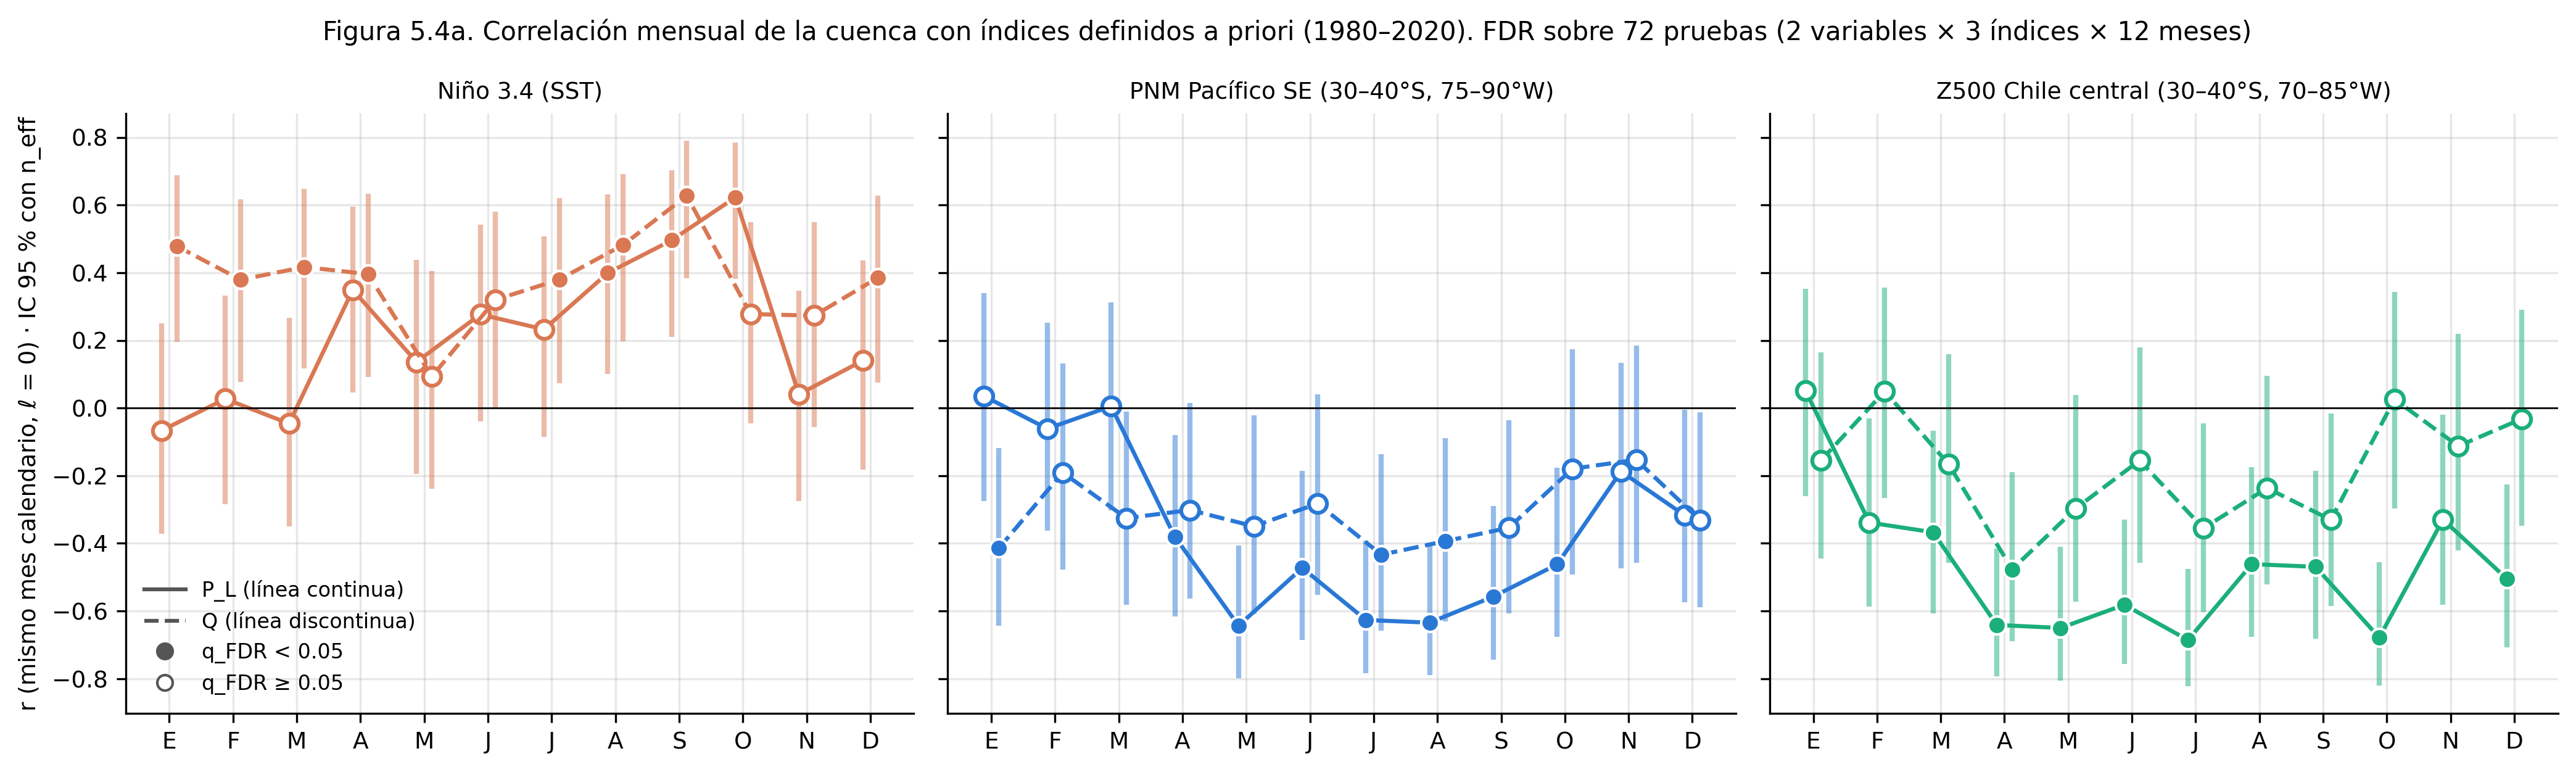
\includegraphics[width=\textwidth]{figura_5_4a_perfiles_indices.png}
\caption{Correlación mensual de $\PL$ (continua) y $\Qm$ (discontinua) con los tres índices; IC del 95\,\% con $n_{\mathrm{eff}}$; relleno si $q_{\mathrm{FDR}}<0.05$ (72 pruebas). Script \archivo{19_p5_4_interpretacion.py}.}
\label{fig:perfiles}
\end{figure}

\paragraph{Regiones, signos y estaciones.} El resultado más sólido es \emph{local y atmosférico}. Entre abril y octubre, $\PL$ se asocia con baja presión frente a Chile central ($r$ de $-0.38$ a $-0.64$) y con baja Z500 sobre la región ($r$ de $-0.46$ a $-0.69$); 16 de las 24 pruebas de PNM y Z500 con $\PL$ son significativas tras el FDR, incluidas las 14 de abril a octubre. Proponemos este mecanismo: cuando el anticiclón subtropical se debilita o se desplaza al norte y una vaguada se instala frente a la costa, los sistemas frontales y las bajas segregadas alcanzan los 33--34$^\circ$S y descargan precipitación reforzada por la orografía \citep{FalveyGarreaud2007,Garreaud2009}. El centro de signo opuesto en altas latitudes (Figura~\ref{fig:todos}) sugiere un patrón de tipo Modo Anular del Sur, cuya fase positiva desplaza los oestes hacia el sur y seca Chile central \citep{Gillett2006}. Es una hipótesis compatible con los mapas, pero no la probamos con un índice SAM. La asociación con la SST tropical es \emph{más débil y tardía}: $\PL$ con Niño 3.4 solo es significativa en agosto--octubre ($r=0.40$, 0.50 y 0.62), coherente con la estacionalidad documentada de la señal de ENSO en Chile central, más fuerte hacia fines del invierno y en primavera \citep{Montecinos2003,Rutllant1991}.

\paragraph{¿Apoyan los patrones atmosféricos la explicación de la SST?} Parcialmente, y los campos no son independientes. Niño 3.4 y la PNM local covarían ($r$ de $-0.28$ a $-0.49$ entre julio y diciembre). Al controlar por la PNM, la correlación parcial de $\PL$ con Niño 3.4 baja (agosto: de 0.40 a 0.20; octubre: de 0.62 a 0.52). La de $\PL$ con la PNM, en cambio, casi no cambia al controlar por Niño 3.4 (julio: de $-0.63$ a $-0.60$). La lectura es que ENSO actúa en buena parte \emph{a través} de la circulación local: El Niño debilita el anticiclón y favorece bloqueos en el Pacífico sureste \citep{Rutllant1991,Montecinos2003}. Esa circulación también varía por causas ajenas a ENSO, y las correlaciones separadas no son influencias independientes.

\paragraph{¿Coinciden los meses de mayor asociación para lluvia y caudal? ¿Es compatible el rezago?} No coinciden, y la diferencia es informativa. $\Qm$ se asocia positivamente con Niño 3.4 \emph{casi todo el año} ($r$ de 0.27 a 0.63 en 11 meses; 8 meses significativos tras el FDR), incluso en verano, cuando casi no llueve. La excepción es mayo ($r=0.09$), el mes de caudal mínimo y más alejado del deshielo. La Figura~\ref{fig:rezagos5} explica la asociación de verano: el caudal de octubre a marzo se correlaciona fuertemente con la lluvia de mayo--agosto previa ($r=0.83$--0.92, $n=37$--39) y más débilmente con el Niño 3.4 de ese invierno ($r=0.29$--0.42; \archivo{figuras/tabla_5_4_memoria_nival.csv}). Esto respalda la cadena \emph{ENSO $\rightarrow$ lluvia invernal $\rightarrow$ nieve $\rightarrow$ caudal de deshielo}, y con ella la hipótesis H-d del punto 1. El rezago de 6 meses es físicamente coherente, pero no supera a la correlación simultánea porque Niño 3.4 persiste varios meses. Son asociaciones; no evaluamos capacidad de pronóstico fuera de muestra.

\begin{figure}[H]
\centering
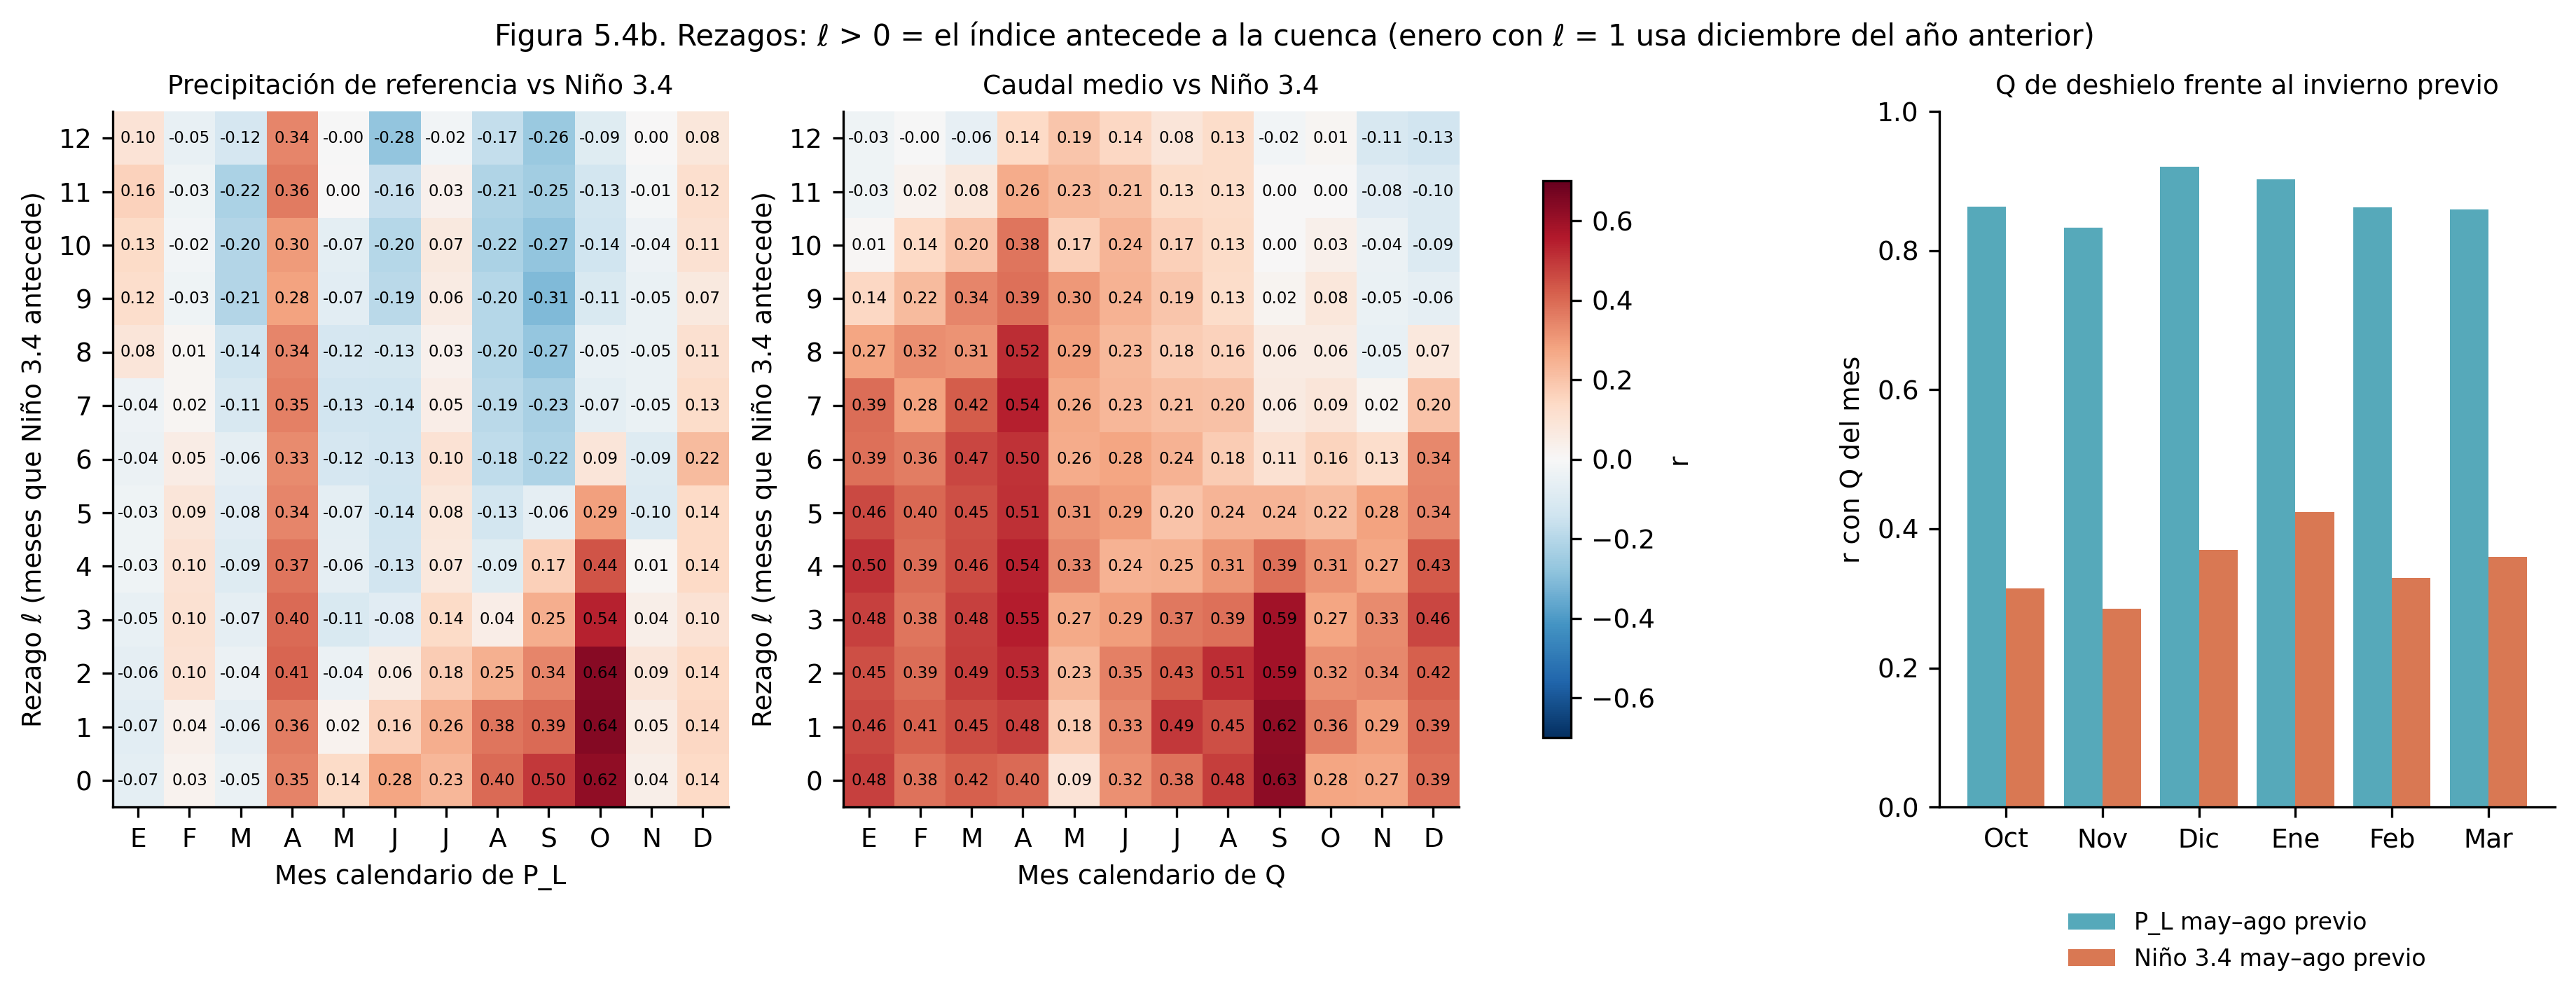
\includegraphics[width=\textwidth]{figura_5_4b_rezagos_nino34.png}
\caption{Correlación de $\PL$ y $\Qm$ con Niño 3.4 por mes y rezago, y caudal de deshielo frente a la lluvia y a Niño 3.4 del invierno previo.}
\label{fig:rezagos5}
\end{figure}

\paragraph{No estacionariedad.} La relación entre la PNM local y $\PL$ es estable en pleno invierno (mayo--agosto: de $-0.41$ a $-0.74$ en 1980--1999 y de $-0.49$ a $-0.59$ en 2000--2019), pero se debilita en septiembre--octubre. La relación entre $\Qm$ y Niño 3.4 \emph{cae} con fuerza después de 2000 (septiembre: de 0.81 a 0.31; enero: de 0.74 a 0.14; Figura~\ref{fig:sub5}). La explicación más plausible es la megasequía: entre 2010 y 2019 la lluvia y el caudal fueron bajos con independencia de la fase de ENSO, y el Niño intenso de 2015 no trajo la lluvia esperada \citep{Garreaud2017,Garreaud2020}. Un control de baja frecuencia (el Pacífico extratropical o la tendencia del Modo Anular del Sur) pudo superponerse a ENSO, aunque con 20 años por subperiodo no podemos separar ese cambio real del ruido muestral.

\paragraph{Relación con las bandas del punto 4.} El punto 4 no encontró un pico interanual robusto: la varianza interanual del caudal es una banda ancha de ruido rojo. En coherencia, la coherencia espectral entre las anomalías de la cuenca y Niño 3.4 es moderada: media de 0.30 ($\PL$) y 0.23 ($\Qm$) en la banda de 2--7 años, con máximos de 0.44--0.46 cerca de 5 años que apenas superan el umbral aproximado del 95\,\% (0.39) (Figura~\ref{fig:coh5}). Compartir la banda de ENSO no demuestra una conexión causal. La sustentan la combinación de un mecanismo conocido, los patrones espaciales coherentes y la cadena de rezagos.

\begin{purplebox}[title={Síntesis de los puntos 4 y 5}]
\textbf{Resultados sólidos.} (1) La escala dominante es el ciclo anual. La variabilidad interanual del caudal es una banda ancha y roja, filtrada por el almacenamiento. (2) La lluvia de abril a octubre se asocia con baja presión y vaguada frente a Chile central (PNM y Z500; $|r|\approx0.5$--0.7, significativa tras el FDR y estable en pleno invierno en ambos subperiodos). (3) Las asociaciones con la SST no dependen del producto (ERA5 frente a ERSST v5).\\[2pt]
\textbf{Asociaciones exploratorias.} (4) ENSO se asocia con la lluvia de agosto a octubre y con el caudal de casi todo el año, transmitido por la nieve; actúa en parte a través de la circulación local y su señal se debilitó después de 2000. (5) Un dipolo de PNM en altas latitudes, compatible con el Modo Anular del Sur.\\[2pt]
\textbf{No comprobado o ausente.} El papel causal del Modo Anular del Sur o del Pacífico extratropical en la megasequía, y cualquier capacidad de pronóstico. No hubo patrones claros de la Z500 con el caudal ni de la SST con la lluvia de verano.
\end{purplebox}
\subsection{Síntesis física de la caracterización}
\label{sec:sintesis}

La Figura~\ref{fig:esquema} es nuestro esquema conceptual de la cuenca. Conecta la circulación regional, la entrada de precipitación, los almacenamientos, las pérdidas y el caudal, e indica las escalas temporales y las cifras que sustentan cada enlace. La Tabla~\ref{tab:evidencias} resume cada resultado principal con su mecanismo propuesto, la evidencia propia, la fuente consultada y su limitación o explicación alternativa.

\begin{figure}[H]
\centering
\begin{tikzpicture}[
  font=\footnotesize,
  caja/.style={draw=mainpurple, rounded corners=3pt, line width=0.8pt, align=center, inner sep=4pt, text width=#1},
  caja/.default=3.0cm,
  flecha/.style={-{Stealth[length=2.6mm]}, line width=0.9pt, mainpurple},
  flechad/.style={-{Stealth[length=2.6mm]}, line width=0.9pt, mainpurple, dashed},
  et/.style={font=\scriptsize, align=center, fill=white, inner sep=1pt, text=darktext}
]
% Fila 1: forzantes, circulación, entrada y pérdidas
\node[caja, fill=bgpurple] (enso) at (1.6,0) {\textbf{Pacífico tropical}\\ENSO (Niño 3.4): El Niño debilita el anticiclón\\\emph{2--7 años}};
\node[caja, fill=bgpurple] (sam) at (1.6,-2.4) {\textbf{Latitudes altas}\\dipolo de PNM tipo SAM\\\emph{hipótesis no probada}};
\node[caja, fill=bgpurple] (circ) at (5.7,-1.2) {\textbf{Circulación regional}\\anticiclón débil o al norte; vaguada en 500~hPa\\$r(\PL,\mathrm{PNM})$: $-0.38$ a $-0.64$};
\node[caja, fill=snowblue] (prec) at (9.8,-1.2) {\textbf{Precipitación invernal}\\frentes + orografía\\may--ago: 70\,\% del total\\$SI_P=0.75$; $r_1=0.15$};
\node[caja, fill=white] (et) at (13.9,-1.2) {\textbf{Pérdidas}\\ET y sublimación bajas (asincronía lluvia--energía)\\$R/P\approx0.88$};
% Fila 2: temperatura y almacenamientos
\node[caja, fill=white] (tem) at (1.6,-5.2) {\textbf{Temperatura}\\isoterma de 0~$^\circ$C: 2900~m (jul) a 4900~m (ene)\\CR2MET: $+0.18$~$^\circ$C/déc.};
\node[caja, fill=snowblue] (nieve) at (5.7,-5.2) {\textbf{Manto nival}\\46--78\,\% de P sobre área $<0$~$^\circ$C\\60\,\% del área $>3000$~m\\\emph{4--7 meses}};
\node[caja, fill=snowblue] (glaciar) at (9.8,-5.2) {\textbf{Glaciares}\\7.2\,\% del área\\verano y años secos ($R/P>1$)};
\node[caja, fill=soilbrown] (subt) at (13.9,-5.2) {\textbf{Agua subterránea}\\BFI $=0.81$\\estiaje $\geq25$~m$^3$/s\\\emph{interanual}};
% Fila 3: salida, intervención y escalas
\node[caja=3.6cm, fill=riverteal] (q) at (9.8,-9.0) {\textbf{Caudal en El Manzano}\\máx. nov--ene (32 de 32 años)\\desfase $\approx6$ meses; $r_1=0.83$\\$-18$~m$^3$/s por década};
\node[caja, fill=white] (reg) at (13.9,-9.0) {\textbf{Intervención}\\El Yeso, centrales, derechos del 20\,\% de $\bar Q$\\\emph{no cuantificada}};
\node[caja=5.6cm, fill=bgpurple, align=left] (esc) at (3.2,-9.0) {\textbf{Escalas temporales}\\[1pt]
\textbullet~días--semanas: sistemas frontales\\
\textbullet~4--7 meses: nieve $\rightarrow$ deshielo\\
\textbullet~1--5 años: ENSO, agua subterránea, glaciares\\
\textbullet~décadas: megasequía y tendencia (2007--2010)};
% Flechas
\draw[flecha] (enso) -- (circ);
\draw[flechad] (sam) -- (circ);
\draw[flecha] (circ) -- (prec);
\draw[flecha] (prec) -- (et);
\draw[flecha] (prec) -- node[et, pos=0.45] {acumulación\\may--sep} (nieve);
\draw[flecha] (prec) -- (glaciar);
\draw[flecha] (prec) -- node[et, pos=0.45] {infiltración} (subt);
\draw[flecha] (tem) -- node[et, above] {deshielo} (nieve);
\draw[flecha] (nieve) -- node[et, pos=0.5] {memoria nival\\$r=0.84$--$0.92$} (q);
\draw[flecha] (glaciar) -- node[et] {fusión} (q);
\draw[flecha] (subt) -- node[et] {flujo base} (q);
\draw[flechad] (reg) -- (q);
\end{tikzpicture}
\caption{Esquema conceptual de la cuenca del Río Maipo en El Manzano. Línea continua: enlaces sustentados por datos propios; discontinua: asociaciones exploratorias o hipótesis no cuantificadas. Las cifras provienen de las Secciones~\ref{sec:p1}--\ref{sec:p5}.}
\label{fig:esquema}
\end{figure}

\begin{table}[H]
\centering\scriptsize
\caption{Tabla de evidencias: resultado principal, mecanismo propuesto, evidencia propia, fuente consultada y limitación o alternativa.}
\label{tab:evidencias}
\begin{tabularx}{\textwidth}{>{\raggedright\arraybackslash}p{2.6cm}>{\raggedright\arraybackslash}X>{\raggedright\arraybackslash}X>{\raggedright\arraybackslash}p{2.0cm}>{\raggedright\arraybackslash}X}
\toprule
Resultado & Mecanismo propuesto & Evidencia propia & Fuente & Limitación o alternativa \\
\midrule
Lluvia unimodal invernal (may--ago, 70\,\%) & Migración estacional del anticiclón subtropical; frentes con realce orográfico & Climatología 2000--2020; máximo may--ago en el 78\,\% de los años; $SI_P=0.75$ & \citep{FalveyGarreaud2007,Viale2011,Garreaud2009} & $\PL$ es un producto grillado; posible subestimación en altura \\
Caudal máximo en dic--ene, desfase de 6 meses & Acumulación nival bajo la isoterma de 0~$^\circ$C y deshielo cuando sube & Máximo de $\Qm$ en nov--ene en 32 de 32 años; 54--64\,\% del área bajo cero en jun--ago; rezago óptimo de 6--7 meses & \citep{Masiokas2006,AlvarezGarreton2018} & Gradiente vertical supuesto; el rezago óptimo surge de una búsqueda entre 13 rezagos \\
$R/P\approx0.88$; $R/P>1$ en años secos & ET baja por asincronía lluvia--energía; liberación de almacenamiento (nieve, glaciar, agua subterránea) & Balance anual por año hidrológico; BFI de 0.81; estiaje $\geq25$~m$^3$/s & \citep{Ayala2020,AlvarezGarreton2021} & $\PL$ podría subestimar la lluvia de altura \\
IMERG atenúa los extremos (Q4: $-52$~mm/mes) & Dificultad para estimar precipitación sólida y orográfica; ajuste con red escasa & 238 pares; error por estación y por cuartil & \citep{Rojas2021,Zambrano2017,Tian2018} & CR2MET también es una estimación; las fuentes comparten pluviómetros \\
Anomalía de lluvia rezagada mejora la predicción del caudal & Memoria nival e hídrica & Menor MAE y RMSE en 3 de 3 bloques externos con ambas fuentes & \citep{Klemes1986,AlvarezGarreton2021} & Sesgo positivo; los bloques no son réplicas independientes \\
Caudal $-18$~m$^3$/s por década en los 12 meses; lluvia invernal en descenso & Megasequía: menos nieve y menos deshielo & OLS-HAC, MK de Hamed--Rao y FDR; elasticidad $\approx1.1$; cambio 2007--2010 & \citep{Garreaud2017,Garreaud2020,Amirthanathan2023} & Sin 2010--2019 no hay tendencia; variabilidad decadal; extracciones \\
Déficit adicional de caudal después de 2010 & Agotamiento de almacenamientos y posible calentamiento de verano y otoño & Residuo de $-30$~mm/año; $T$ CR2MET $+0.18$~$^\circ$C por década, nulo en invierno & \citep{AlvarezGarreton2021,Falvey2009} & Ocho años; temperaturas de producto, no de estación \\
Caudal con espectro rojo; lluvia casi blanca & Filtro pasa-bajos del almacenamiento & $r_1$ de 0.15 frente a 0.83; 62\,\% de varianza interanual en $\Qm$ & \citep{Gilman1963,Torrence1998} & La regulación también suaviza; sin datos de operación \\
Sin periodicidades interanuales significativas & Variabilidad de banda ancha; ENSO no es periódico & Ningún pico supera el umbral global del AR(1) & \citep{Trenberth1997} & Registro de 40 años; pocos ciclos por periodo \\
Lluvia invernal ligada a la circulación local (PNM y Z500) & Bloqueo o paso de los frentes; vaguadas y bajas segregadas & 16 de 24 pruebas significativas tras FDR; estable en pleno invierno & \citep{Garreaud2009,Montecinos2003} & Correlación, no causalidad; posible influencia del SAM \\
Caudal ligado a ENSO casi todo el año & ENSO $\rightarrow$ lluvia invernal $\rightarrow$ nieve $\rightarrow$ deshielo & 8 meses significativos; memoria nival $r=0.83$--0.92; igual con ERSST & \citep{Montecinos2003,Rutllant1991,Cortes2017} & Señal debilitada después de 2000; sin evaluación de pronóstico \\
\bottomrule
\end{tabularx}
\end{table}

% =============================================================================
\section{Conclusiones}
\label{sec:conclusiones}
% =============================================================================

\begin{enumerate}
\item \textbf{Clasificación.} El Río Maipo en El Manzano tiene un \emph{régimen nival de montaña mediterránea con almacenamiento estacional e interanual}. La lluvia llega en invierno (may--ago, 70\,\% del total) con los sistemas frontales que el anticiclón subtropical deja pasar. Se almacena sobre todo como nieve: de junio a agosto la isoterma de 0~$^\circ$C baja a 2900--3100~m y deja bajo cero más de la mitad de una cuenca cuyo 60\,\% está sobre 3000~m. Sale como caudal en primavera--verano, con el máximo en diciembre--enero y seis meses de desfase. La clasificación es estable en los dos subperiodos y en casi todos los años.
\item \textbf{Relaciones.} IMERG reproduce la variabilidad de la referencia, pero subestima los inviernos intensos; corregirlo estadísticamente no mejora la estimación fuera del ajuste. La relación aprovechable entre lluvia y caudal es retardada: la anomalía de lluvia de 6--7 meses antes mejora la estimación del caudal frente a la climatología.
\item \textbf{Cambios.} El caudal disminuye en los doce meses ($-18$~m$^3$/s por década), con mayor magnitud en el deshielo, en proporción al descenso de la lluvia invernal de la megasequía. El cambio se concentra después de 2007--2010 y no se distingue de un salto de nivel. La explicación mejor sustentada es el déficit de precipitación invernal transmitido por la nieve, con un posible déficit adicional por agotamiento de almacenamientos. La temperatura de la base aumenta 0.18~$^\circ$C por década, pero casi nada en invierno, por lo que el calentamiento es un candidato para el déficit residual y no la causa principal; la regulación queda como hipótesis abierta.
\item \textbf{Escalas.} El ciclo anual es la única periodicidad robusta. La cuenca convierte una lluvia mensual casi sin memoria en un caudal con fuerte persistencia interanual, la huella espectral de su almacenamiento.
\item \textbf{Clima global.} La lluvia invernal depende sobre todo de la circulación regional frente a Chile central. ENSO la modula a fines del invierno, en parte a través de esa circulación, y su señal pasa al caudal de casi todo el año por la memoria nival, con el mismo resultado usando ERA5 o ERSST. Esa conexión no fue estacionaria: se debilitó durante la megasequía.
\end{enumerate}

\paragraph{Revisión de la hipótesis inicial.} \emph{Se mantuvo} el núcleo nival: el desfase, el almacenamiento, el espectro rojo del caudal y la transmisión de la señal invernal al verano se confirmaron con evidencia independiente en los cinco puntos. \emph{Cambió} el papel de ENSO: no es el control principal de la lluvia mensual, sino un modulador tardío y no estacionario, mientras que la circulación regional explica más varianza y de forma más estable. También \emph{se añadió} un componente que la hipótesis no contemplaba: un descenso de largo plazo del agua disponible, concentrado después de 2007--2010, cuya atribución a una causa específica no es posible con estos datos. Las principales incertidumbres son la representatividad de la precipitación y la temperatura en alta montaña (productos grillados y de reanálisis), la ausencia de datos de nieve, de operación del embalse y de extracciones, y la longitud del registro frente a la variabilidad decadal.

\subsection{Limitaciones y mejoras pendientes}
\label{sec:limitaciones}
\begin{itemize}
\item Las dos temperaturas difieren 5.6~$^\circ$C en su nivel medio y no hay estaciones de altura para decidir cuál es correcta; la fracción de precipitación sobre área bajo cero queda acotada entre 46 y 78\,\%. ERA5-Land se extrajo solo para 2000--2020, aunque existe desde 1950; extenderlo permitiría comparar las tendencias térmicas en 40 años.
\item La isoterma de 0~$^\circ$C supone un gradiente vertical uniforme, sin inversiones térmicas ni efectos de orientación, y una precipitación uniforme en la cuenca.
\item No se conservó el manifiesto de la exportación de IMERG; la versión se documenta como V06 según la configuración del script, y los valores usados se entregan en \archivo{datos/datos_satelitales_imerg_era5.csv}.
\item No se evaluó la persistencia de largo plazo (MK4) ni la significancia regional de las tendencias.
\item Las asociaciones del punto 5 son simultáneas; ninguna afirmación es predictiva.
\end{itemize}

% =============================================================================
\section{Uso de inteligencia artificial}
\label{sec:ia}
% =============================================================================

Aplicamos el Nivel A (abierto) de la política de IA del curso. Todas las sesiones con IA quedaron registradas en \archivo{BITACORA_AGENTES.md} con fecha, integrante, herramienta, tareas, validaciones y próximos pasos, siguiendo el protocolo de \archivo{AGENTS.md}.

\paragraph{1. Herramientas y versiones.} GitHub Copilot en VS Code (Santiago Ortega Ruiz; Bryan Alexander Salazar Castañeda, para preparar la descarga ERA5; tareas del dashboard); Antigravity de Google DeepMind (Mateo Arango Cortés; revisiones cruzadas y corrección del dashboard, registrada con el modelo Gemini 3.8 Flash); y Claude Code con el modelo Claude Opus 5.5, en la extensión de VS Code (Tomás Gómez Zuleta: puntos 3 y 4, apoyo al punto 5 y ensamblaje de este informe; Santiago Ortega Ruiz: versión final del paquete, verificación de referencias, criterio de completitud, temperatura de la base, isoterma de 0~$^\circ$C, contraste con ERSST y reproducción completa). La versión exacta del modelo de Copilot no quedó registrada.

\paragraph{2. Tareas en las que intervino la IA.} Programación y depuración de los scripts de análisis y de figuras; propuestas de métodos (errores HAC, corrección de Hamed--Rao, FDR, umbrales AR(1) por Monte Carlo, $n_{\mathrm{eff}}$ de Bretherton); configuración de la descarga del CDS; construcción del dashboard; búsqueda orientativa de bibliografía; y redacción y edición de los documentos \LaTeX{} y de este informe.

\paragraph{3. Resultados verificados y cómo.} (i) Conversión de caudal a lámina comprobada a mano (mayo de 1980). (ii) Invarianza de la pendiente OLS frente a la anomalización y la estandarización, verificada numéricamente (diferencia $<10^{-13}$). (iii) Parseval verificado en todos los espectros (cociente 1.00). (iv) Media 0 y desviación 1 de $a$ y $z$ en la referencia, para los 48 pares variable--mes. (v) Campos ERA5 revisados en dimensiones, fechas, unidades y rangos físicos (\texttt{--verify} del script 15). (vi) Completitud diaria recalculada desde los archivos originales de CAMELS-CL. (vii) DOI de las referencias comprobados uno a uno contra Crossref, DataCite y \texttt{doi.org}, comparando autor, título, año, volumen y páginas; también se verificó que cada referencia se cita en el texto. (viii) La temperatura mensual del CSV maestro coincide con CR2MET recalculado desde los archivos diarios (script 21). (ix) Reproducción completa: el paquete entregado se descomprimió en una carpeta aparte y los scripts se ejecutaron en un entorno virtual limpio con \archivo{requirements.txt}; las tablas coinciden con las entregadas salvo diferencias de redondeo menores que $10^{-9}$.

\paragraph{4. Propuestas corregidas o rechazadas.} (a) La etiqueta ``IMERG V07'' de un registro inicial se corrigió a V06, conforme al script. (b) El factor de Hamed--Rao producía factores menores que 1, lo que \emph{reduciría} la varianza; se acotó a $\geq1$. (c) Un promedio en precisión simple (\texttt{float32}) de \texttt{xarray} sesgaba las anomalías de los campos; se forzó \texttt{float64}. (d) La SST bajo hielo marino generaba artefactos; se enmascaró. (e) Se resolvieron conflictos de \texttt{git} que rompían el dashboard. (f) Al ensamblar este informe, la verificación contra Crossref detectó DOI que la propia IA había escrito mal: cuatro en las notas de las tablas de extremos y de síntesis del punto 1 (por ejemplo, el atribuido a Garreaud et al. 2017 correspondía a otro artículo) y el de Gilman et al. en el documento del punto 4. Se corrigieron en \archivo{scripts/07_rol_a_explorador.py}, en las tablas regeneradas y en el borrador del punto 4. (g) Se descartó la afirmación de que el caudal de mayo de 1993 era un valor mensual representativo, al comprobar que promedia solo tres días. (h) Se descartó afirmar ``seis meses bajo cero'' como criterio de clasificación, porque depende del producto de temperatura; se reemplazó por la isoterma de 0~$^\circ$C con los dos productos. (i) El archivo de dependencias propuesto inicialmente fijaba \texttt{pandas} 3.0, incompatible con \texttt{statsmodels} 0.14.5; la prueba en un entorno limpio lo detectó y se fijó \texttt{pandas} 2.3.3. (j) Al aplicar el criterio de completitud, la coherencia con Niño 3.4 dejó de calcularse porque la interpolación tenía un límite de 8 meses y el vacío de 2015 es de 10; se igualó al tratamiento del punto 4. (k) El balance anual del punto 3.6 se había calculado fuera de los scripts; se escribió \archivo{scripts/25_p3_6_balance_anual.py} para que sea reproducible.

\paragraph{5. Contribuciones de los integrantes.} \emph{Mateo Arango Cortés}: datos de la fase 1, punto 1 (exploración, control de calidad, climatología y clasificación) y su documento. \emph{Santiago Ortega Ruiz}: punto 2 (relaciones, rezagos y validación cronológica), auditorías de IMERG y su documento; versión final del paquete de entrega (criterio de completitud, temperatura CR2MET, isoterma de 0~$^\circ$C, contraste con ERSST, balance anual y verificación de la reproducibilidad). \emph{Tomás Gómez Zuleta}: puntos 3 y 4 (tendencias, robustez, causas y Fourier), apoyo al punto 5 (descarga ERA5, mapas, robustez e interpretación), mapas de la cuenca, auditoría diaria y ensamblaje de este informe. \emph{Bryan Alexander Salazar Castañeda}: planteamiento del punto 5, preparación de la descarga ERA5 y edición. Los cuatro integrantes revisaron los resultados de los demás puntos mediante la bitácora.
% =============================================================================
% REFERENCIAS — DOI comprobados contra Crossref, DataCite y doi.org (octubre de 2026)
% =============================================================================
\renewcommand{\refname}{Referencias}
\begin{thebibliography}{99}\small
\setlength{\itemsep}{1pt}

\bibitem{AlvarezGarreton2018} Alvarez-Garreton, C., Mendoza, P. A., Boisier, J. P., Addor, N., Galleguillos, M., Zambrano-Bigiarini, M., et al. (2018). The CAMELS-CL dataset: catchment attributes and meteorology for large sample studies -- Chile dataset. \emph{Hydrology and Earth System Sciences}, 22, 5817--5846. \url{https://doi.org/10.5194/hess-22-5817-2018}

\bibitem{AlvarezGarreton2021} Alvarez-Garreton, C., Boisier, J. P., Garreaud, R., Seibert, J., y Vis, M. (2021). Progressive water deficits during multiyear droughts in basins with long hydrological memory in Chile. \emph{Hydrology and Earth System Sciences}, 25, 429--446. \url{https://doi.org/10.5194/hess-25-429-2021}

\bibitem{Amirthanathan2023} Amirthanathan, G. E., Bari, M. A., Woldemeskel, F. M., Tuteja, N. K., y Feikema, P. M. (2023). Regional significance of historical trends and step changes in Australian streamflow. \emph{Hydrology and Earth System Sciences}, 27, 229--254. \url{https://doi.org/10.5194/hess-27-229-2023}

\bibitem{ASTERGDEM} NASA/METI/AIST/Japan Spacesystems y U.S./Japan ASTER Science Team (2019). ASTER Global Digital Elevation Model V003. NASA Land Processes Distributed Active Archive Center. \url{https://doi.org/10.5067/ASTER/ASTGTM.003}

\bibitem{Ayala2020} Ayala, A., Farías-Barahona, D., Huss, M., Pellicciotti, F., McPhee, J., y Farinotti, D. (2020). Glacier runoff variations since 1955 in the Maipo River basin, in the semiarid Andes of central Chile. \emph{The Cryosphere}, 14, 2005--2027. \url{https://doi.org/10.5194/tc-14-2005-2020}

\bibitem{BH1995} Benjamini, Y., y Hochberg, Y. (1995). Controlling the false discovery rate: a practical and powerful approach to multiple testing. \emph{Journal of the Royal Statistical Society: Series B}, 57, 289--300. \url{https://doi.org/10.1111/j.2517-6161.1995.tb02031.x}

\bibitem{Bergmeir2018} Bergmeir, C., Hyndman, R. J., y Koo, B. (2018). A note on the validity of cross-validation for evaluating autoregressive time series prediction. \emph{Computational Statistics \& Data Analysis}, 120, 70--83. \url{https://doi.org/10.1016/j.csda.2017.11.003}

\bibitem{Boisier2016} Boisier, J. P., Rondanelli, R., Garreaud, R. D., y Muñoz, F. (2016). Anthropogenic and natural contributions to the Southeast Pacific precipitation decline and recent megadrought in central Chile. \emph{Geophysical Research Letters}, 43, 413--421. \url{https://doi.org/10.1002/2015GL067265}

\bibitem{Bretherton1999} Bretherton, C. S., Widmann, M., Dymnikov, V. P., Wallace, J. M., y Bladé, I. (1999). The effective number of spatial degrees of freedom of a time-varying field. \emph{Journal of Climate}, 12, 1990--2009. \url{https://doi.org/10.1175/1520-0442(1999)012<1990:TENOSD>2.0.CO;2}

\bibitem{Cleveland1979} Cleveland, W. S. (1979). Robust locally weighted regression and smoothing scatterplots. \emph{Journal of the American Statistical Association}, 74, 829--836. \url{https://doi.org/10.1080/01621459.1979.10481038}

\bibitem{Cortes2017} Cortés, G., y Margulis, S. (2017). Impacts of El Niño and La Niña on interannual snow accumulation in the Andes: Results from a high-resolution 31 year reanalysis. \emph{Geophysical Research Letters}, 44, 6859--6867. \url{https://doi.org/10.1002/2017GL073826}

\bibitem{ERA5single} Hersbach, H., Bell, B., Berrisford, P., et al. (2019). ERA5 monthly averaged data on single levels from 1940 to present. Copernicus Climate Change Service (C3S) Climate Data Store. \url{https://doi.org/10.24381/cds.f17050d7} (consultado en octubre de 2026).

\bibitem{ERA5pressure} Hersbach, H., Bell, B., Berrisford, P., et al. (2019). ERA5 monthly averaged data on pressure levels from 1940 to present. Copernicus Climate Change Service (C3S) Climate Data Store. \url{https://doi.org/10.24381/cds.6860a573} (consultado en octubre de 2026).

\bibitem{Falvey2009} Falvey, M., y Garreaud, R. D. (2009). Regional cooling in a warming world: Recent temperature trends in the southeast Pacific and along the west coast of subtropical South America (1979--2006). \emph{Journal of Geophysical Research: Atmospheres}, 114, D04102. \url{https://doi.org/10.1029/2008JD010519}

\bibitem{FalveyGarreaud2007} Falvey, M., y Garreaud, R. (2007). Wintertime precipitation episodes in central Chile: Associated meteorological conditions and orographic influences. \emph{Journal of Hydrometeorology}, 8, 171--193. \url{https://doi.org/10.1175/JHM562.1}

\bibitem{Garreaud2009} Garreaud, R. D., Vuille, M., Compagnucci, R., y Marengo, J. (2009). Present-day South American climate. \emph{Palaeogeography, Palaeoclimatology, Palaeoecology}, 281, 180--195. \url{https://doi.org/10.1016/j.palaeo.2007.10.032}

\bibitem{Garreaud2017} Garreaud, R. D., Alvarez-Garreton, C., Barichivich, J., Boisier, J. P., Christie, D., Galleguillos, M., et al. (2017). The 2010--2015 megadrought in central Chile: impacts on regional hydroclimate and vegetation. \emph{Hydrology and Earth System Sciences}, 21, 6307--6327. \url{https://doi.org/10.5194/hess-21-6307-2017}

\bibitem{Garreaud2020} Garreaud, R. D., Boisier, J. P., Rondanelli, R., Montecinos, A., Sepúlveda, H. H., y Veloso-Aguila, D. (2020). The Central Chile Mega Drought (2010--2018): A climate dynamics perspective. \emph{International Journal of Climatology}, 40, 421--439. \url{https://doi.org/10.1002/joc.6219}

\bibitem{Gillett2006} Gillett, N. P., Kell, T. D., y Jones, P. D. (2006). Regional climate impacts of the Southern Annular Mode. \emph{Geophysical Research Letters}, 33, L23704. \url{https://doi.org/10.1029/2006GL027721}

\bibitem{Gilman1963} Gilman, D. L., Fuglister, F. J., y Mitchell, J. M. (1963). On the power spectrum of ``red noise''. \emph{Journal of the Atmospheric Sciences}, 20, 182--184. \url{https://doi.org/10.1175/1520-0469(1963)020<0182:OTPSON>2.0.CO;2}

\bibitem{Gupta2009} Gupta, H. V., Kling, H., Yilmaz, K. K., y Martinez, G. F. (2009). Decomposition of the mean squared error and NSE performance criteria: Implications for improving hydrological modelling. \emph{Journal of Hydrology}, 377, 80--91. \url{https://doi.org/10.1016/j.jhydrol.2009.08.003}

\bibitem{HamedRao1998} Hamed, K. H., y Rao, A. R. (1998). A modified Mann--Kendall trend test for autocorrelated data. \emph{Journal of Hydrology}, 204, 182--196. \url{https://doi.org/10.1016/S0022-1694(97)00125-X}

\bibitem{Harris1978} Harris, F. J. (1978). On the use of windows for harmonic analysis with the discrete Fourier transform. \emph{Proceedings of the IEEE}, 66, 51--83. \url{https://doi.org/10.1109/PROC.1978.10837}

\bibitem{Hersbach2020} Hersbach, H., Bell, B., Berrisford, P., et al. (2020). The ERA5 global reanalysis. \emph{Quarterly Journal of the Royal Meteorological Society}, 146, 1999--2049. \url{https://doi.org/10.1002/qj.3803}

\bibitem{Hirsch1982} Hirsch, R. M., Slack, J. R., y Smith, R. A. (1982). Techniques of trend analysis for monthly water quality data. \emph{Water Resources Research}, 18, 107--121. \url{https://doi.org/10.1029/WR018i001p00107}

\bibitem{HossainHuffman2008} Hossain, F., y Huffman, G. J. (2008). Investigating error metrics for satellite rainfall data at hydrologically relevant scales. \emph{Journal of Hydrometeorology}, 9, 563--575. \url{https://doi.org/10.1175/2007JHM925.1}

\bibitem{Huang2017} Huang, B., Thorne, P. W., Banzon, V. F., Boyer, T., Chepurin, G., Lawrimore, J. H., Menne, M. J., Smith, T. M., Vose, R. S., y Zhang, H.-M. (2017). Extended Reconstructed Sea Surface Temperature, Version 5 (ERSSTv5): upgrades, validations, and intercomparisons. \emph{Journal of Climate}, 30, 8179--8205. \url{https://doi.org/10.1175/JCLI-D-16-0836.1}. Datos: NOAA NCEI, \url{https://doi.org/10.7289/V5T72FNM}

\bibitem{Huffman2020} Huffman, G. J., Bolvin, D. T., Braithwaite, D., Hsu, K.-L., Joyce, R. J., Kidd, C., Nelkin, E. J., Sorooshian, S., et al. (2020). Integrated Multi-satellite Retrievals for the Global Precipitation Measurement (GPM) Mission (IMERG). En V. Levizzani et al. (Eds.), \emph{Satellite Precipitation Measurement}, Advances in Global Change Research, 67, 343--353. Springer. \url{https://doi.org/10.1007/978-3-030-24568-9_19}

\bibitem{IMERGV06} Huffman, G. J., Stocker, E. F., Bolvin, D. T., Nelkin, E. J., y Tan, J. (2019). GPM IMERG Final Precipitation L3 1 month 0.1 degree x 0.1 degree V06. Goddard Earth Sciences Data and Information Services Center (GES DISC). \url{https://doi.org/10.5067/GPM/IMERG/3B-MONTH/06}. Accedido mediante Google Earth Engine, colección \texttt{NASA/GPM\_L3/IMERG\_MONTHLY\_V06}.

\bibitem{Kendall1975} Kendall, M. G. (1975). \emph{Rank Correlation Methods} (4.ª ed.). Londres: Charles Griffin.

\bibitem{Klemes1986} Klemeš, V. (1986). Operational testing of hydrological simulation models. \emph{Hydrological Sciences Journal}, 31, 13--24. \url{https://doi.org/10.1080/02626668609491024}

\bibitem{Lomb1976} Lomb, N. R. (1976). Least-squares frequency analysis of unequally spaced data. \emph{Astrophysics and Space Science}, 39, 447--462. \url{https://doi.org/10.1007/BF00648343}

\bibitem{Mann1945} Mann, H. B. (1945). Nonparametric tests against trend. \emph{Econometrica}, 13, 245--259. \url{https://doi.org/10.2307/1907187}

\bibitem{Masiokas2006} Masiokas, M. H., Villalba, R., Luckman, B. H., Le Quesne, C., y Aravena, J. C. (2006). Snowpack variations in the central Andes of Argentina and Chile, 1951--2005: large-scale atmospheric influences and implications for water resources in the region. \emph{Journal of Climate}, 19, 6334--6352. \url{https://doi.org/10.1175/JCLI3969.1}

\bibitem{Montecinos2003} Montecinos, A., y Aceituno, P. (2003). Seasonality of the ENSO-related rainfall variability in central Chile and associated circulation anomalies. \emph{Journal of Climate}, 16, 281--296. \url{https://doi.org/10.1175/1520-0442(2003)016<0281:SOTERR>2.0.CO;2}

\bibitem{MunozSabater2021} Muñoz-Sabater, J., Dutra, E., Agustí-Panareda, A., et al. (2021). ERA5-Land: a state-of-the-art global reanalysis dataset for land applications. \emph{Earth System Science Data}, 13, 4349--4383. \url{https://doi.org/10.5194/essd-13-4349-2021}

\bibitem{NeweyWest1987} Newey, W. K., y West, K. D. (1987). A simple, positive semi-definite, heteroskedasticity and autocorrelation consistent covariance matrix. \emph{Econometrica}, 55, 703--708. \url{https://doi.org/10.2307/1913610}

\bibitem{Pettitt1979} Pettitt, A. N. (1979). A non-parametric approach to the change-point problem. \emph{Applied Statistics}, 28, 126--135. \url{https://doi.org/10.2307/2346729}

\bibitem{PyperPeterman1998} Pyper, B. J., y Peterman, R. M. (1998). Comparison of methods to account for autocorrelation in correlation analyses of fish data. \emph{Canadian Journal of Fisheries and Aquatic Sciences}, 55, 2127--2140. \url{https://doi.org/10.1139/f98-104}

\bibitem{Roberts2017} Roberts, D. R., Bahn, V., Ciuti, S., Boyce, M. S., Elith, J., Guillera-Arroita, G., et al. (2017). Cross-validation strategies for data with temporal, spatial, hierarchical, or phylogenetic structure. \emph{Ecography}, 40, 913--929. \url{https://doi.org/10.1111/ecog.02881}

\bibitem{Rojas2021} Rojas, Y., Minder, J. R., Campbell, L. S., Massmann, A., y Garreaud, R. (2021). Assessment of GPM IMERG satellite precipitation estimation and its dependence on microphysical rain regimes over the mountains of south-central Chile. \emph{Atmospheric Research}, 253, 105454. \url{https://doi.org/10.1016/j.atmosres.2021.105454}

\bibitem{Rutllant1991} Rutllant, J., y Fuenzalida, H. (1991). Synoptic aspects of the central Chile rainfall variability associated with the Southern Oscillation. \emph{International Journal of Climatology}, 11, 63--76. \url{https://doi.org/10.1002/joc.3370110105}

\bibitem{Scargle1982} Scargle, J. D. (1982). Studies in astronomical time series analysis. II. Statistical aspects of spectral analysis of unevenly spaced data. \emph{The Astrophysical Journal}, 263, 835--853. \url{https://doi.org/10.1086/160554}

\bibitem{Sen1968} Sen, P. K. (1968). Estimates of the regression coefficient based on Kendall's tau. \emph{Journal of the American Statistical Association}, 63, 1379--1389. \url{https://doi.org/10.1080/01621459.1968.10480934}

\bibitem{SotoAlvarez2020} Soto-Alvarez, M., Alcayaga, H., Alarcón, V., Caamaño, D., Palma, S., y Escanilla, R. (2020). Evaluation of products 3B42 V7 and 3IMERG for the hydroclimatic regions of Chile. \emph{Journal of South American Earth Sciences}, 104, 102870. \url{https://doi.org/10.1016/j.jsames.2020.102870}

\bibitem{Tian2018} Tian, F., Hou, S., Yang, L., Hu, H., y Hou, A. (2018). How does the evaluation of the GPM IMERG rainfall product depend on gauge density and rainfall intensity? \emph{Journal of Hydrometeorology}, 19, 339--349. \url{https://doi.org/10.1175/JHM-D-17-0161.1}

\bibitem{Torrence1998} Torrence, C., y Compo, G. P. (1998). A practical guide to wavelet analysis. \emph{Bulletin of the American Meteorological Society}, 79, 61--78. \url{https://doi.org/10.1175/1520-0477(1998)079<0061:APGTWA>2.0.CO;2}

\bibitem{Trenberth1997} Trenberth, K. E. (1997). The definition of El Niño. \emph{Bulletin of the American Meteorological Society}, 78, 2771--2777. \url{https://doi.org/10.1175/1520-0477(1997)078<2771:TDOENO>2.0.CO;2}

\bibitem{Viale2011} Viale, M., y Nuñez, M. N. (2011). Climatology of winter orographic precipitation over the subtropical central Andes and associated synoptic and regional characteristics. \emph{Journal of Hydrometeorology}, 12, 481--507. \url{https://doi.org/10.1175/2010JHM1284.1}

\bibitem{WalshLawler1981} Walsh, R. P. D., y Lawler, D. M. (1981). Rainfall seasonality: description, spatial patterns and change through time. \emph{Weather}, 36, 201--208. \url{https://doi.org/10.1002/j.1477-8696.1981.tb05400.x}

\bibitem{Welch1967} Welch, P. D. (1967). The use of fast Fourier transform for the estimation of power spectra: A method based on time averaging over short, modified periodograms. \emph{IEEE Transactions on Audio and Electroacoustics}, 15, 70--73. \url{https://doi.org/10.1109/TAU.1967.1161901}

\bibitem{Wilks2016} Wilks, D. S. (2016). ``The stippling shows statistically significant grid points'': How research results are routinely overstated and overinterpreted, and what to do about it. \emph{Bulletin of the American Meteorological Society}, 97, 2263--2273. \url{https://doi.org/10.1175/BAMS-D-15-00267.1}

\bibitem{Willmott1981} Willmott, C. J. (1981). On the validation of models. \emph{Physical Geography}, 2, 184--194. \url{https://doi.org/10.1080/02723646.1981.10642213}

\bibitem{Zambrano2017} Zambrano-Bigiarini, M., Nauditt, A., Birkel, C., Verbist, K., y Ribbe, L. (2017). Temporal and spatial evaluation of satellite-based rainfall estimates across the complex topographical and climatic gradients of Chile. \emph{Hydrology and Earth System Sciences}, 21, 1295--1320. \url{https://doi.org/10.5194/hess-21-1295-2017}

\end{thebibliography}

% =============================================================================
\appendix
\section{Trazabilidad y reproducción}
\label{sec:anexoA}
% =============================================================================

\paragraph{Orden de ejecución.} Desde la raíz del paquete, con Python 3.13 y las versiones de \archivo{requirements.txt} (numpy 2.3.4, pandas 2.3.3, scipy 1.16.3, statsmodels 0.14.5, matplotlib 3.10.6, xarray 2025.10.1, netCDF4 1.7.3, Pillow 12.0.0), con las que se reprodujo el análisis completo en un entorno limpio; \texttt{cdsapi}, \texttt{earthengine-api} y \texttt{geopandas} solo para volver a descargar datos. Orden: 01, 03 (02 y 15 solo para volver a descargar), 22, 23, 07, 20, 04--06, 09--12, 21, 25, 13, 14, 16--19, 24 y, al final, 08 (dashboard). El \archivo{README.md} del paquete detalla los comandos.

\begin{table}[H]
\centering\footnotesize
\caption{Scripts, entradas y productos. Todas las rutas son relativas a la raíz del paquete.}
\label{tab:trazabilidad}
\begin{tabularx}{\textwidth}{>{\raggedright\arraybackslash}p{4.9cm}>{\raggedright\arraybackslash}X>{\raggedright\arraybackslash}p{2.3cm}}
\toprule
Script & Función y productos principales & Sección \\
\midrule
\archivo{01_preparar_datos.py} & Agrega CAMELS-CL diario a mensual ($\PL$, $\Qm$, $R$, $T$) con el criterio de completitud & \ref{sec:qc} \\
\archivo{02_descargar_satelite.py} & IMERG V06 y ERA5-Land mensuales en Earth Engine (requiere autenticación); salida \archivo{datos/datos_satelitales_imerg_era5.csv} & \ref{sec:datos} \\
\archivo{03_integrar_datos.py} & Unión externa y CSV maestro \archivo{datos/datos_mensuales_maipo.csv} & \ref{sec:datos} \\
\archivo{07_rol_a_explorador.py} & Figuras 1.1--1.7; tablas 1.1--1.6 & \ref{sec:p1} \\
\archivo{22_p1_0_topografia_cuenca.py} & Mapa topográfico, curva hipsométrica y tabla 1.12 (ASTER GDEM v3) & \ref{sec:ficha} \\
\archivo{20_p1_4_auditoria_diaria.py} & Completitud diaria, sensibilidad, ficha y picos por año; figura 1.8; tablas 1.7--1.11 & \ref{sec:ficha}, \ref{sec:qc}, \ref{sec:clim} \\
\archivo{23_p1_5_isoterma_cero.py} & Isoterma de 0~$^\circ$C y área bajo cero (figura 1.9; tablas 1.13--1.14) & \ref{sec:isoterma} \\
\archivo{04_analisis_precipitacion.py} & Dispersión y métricas (figura 2.1; tablas 2.1) & \ref{sec:p2} \\
\archivo{05_anomalias_rezagos.py} & Anomalías y rezagos (figura 2.2; tablas 2.2) & \ref{sec:p2} \\
\archivo{06_modelos_validacion_temporal.py} & Modelos y validación por bloques (figuras 2.3--2.4; tablas 2.3) & \ref{sec:p2} \\
\archivo{09_p3_2_anomalias.py}, \archivo{10_p3_3_escalas_temporales.py} & Anomalías y dos escalas (figuras 3.2 y 3.3) & \ref{sec:p3} \\
\archivo{11_p3_4_metodos_tendencia.py}, \archivo{12_p3_5_incertidumbre_robustez.py} & Métodos, FDR, sensibilidad y salto (figuras 3.4--3.5) & \ref{sec:p3} \\
\archivo{21_p3_1_temperatura_cr2met.py} & Temperatura CR2MET frente a ERA5-Land & \ref{sec:temp}, \ref{sec:p3} \\
\archivo{25_p3_6_balance_anual.py} & Balance por año hidrológico, elasticidad y regresión anual (tablas 3.6) & \ref{sec:p36} \\
\archivo{13_p4_1_preparacion_espectral.py}, \archivo{14_p4_2_espectros_interpretacion.py} & Series espectrales, espectros, AR(1) y estabilidad (figuras 4.1--4.2) & \ref{sec:p4} \\
\archivo{15_p5_1_descargar_campos_era5.py} & Descarga ERA5 del CDS (requiere \archivo{~/.cdsapirc}, que no se entrega) & \ref{sec:p5} \\
\archivo{16_p5_1_campos_climaticos.py} a \archivo{19_p5_4_interpretacion.py} & Climatología de campos, mapas, robustez, índices, rezagos y coherencia (figuras 5.1--5.4) & \ref{sec:p5} \\
\archivo{24_p5_3_contraste_ersst.py} & Contraste ERA5 frente a ERSST v5 (figura 5.5; tablas 5.5) & \ref{sec:ersst} \\
\archivo{08_build_dashboard_data.py} & Dashboard interactivo de apoyo a la exposición (\archivo{dashboard/dashboard_autocontenido.html}) & -- \\
\bottomrule
\end{tabularx}
\end{table}

\paragraph{Datos entregados.} \archivo{datos/datos_mensuales_maipo.csv} (serie maestra mensual), construida a partir de \archivo{datos/datos_mensuales_procesados.csv} (agregación de CAMELS-CL con los días válidos de cada mes) y \archivo{datos/datos_satelitales_imerg_era5.csv} (IMERG y ERA5-Land extraídos de Earth Engine); \archivo{datos/campos_ersst/} (SST ERSST v5 de 2$^\circ$, 1979--2020); \archivo{datos/camels_cl_5710001/} (caudal diario, precipitación y temperaturas diarias CR2MET, atributos y polígono de la cuenca, subconjunto CAMELS-CL usado); \archivo{datos/ASTGTM_003-20261004_142607/} (cuatro teselas ASTER GDEM v3 de 1$^\circ$, S34--S35 y W070--W071, descargadas de NASA Earthdata); \archivo{datos/campos_era5/} (SST, PNM y Z500 mensuales de ERA5, 1979--2020, y línea de costa de Natural Earth para los mapas). Las series procesadas, anomalías y tablas están en \archivo{figuras/} (\texttt{serie\_*.csv} y \texttt{tabla\_*.csv}).

\paragraph{Figuras de la cuenca.} El mapa topográfico y la curva hipsométrica (Figuras~\ref{fig:mapas}b y~\ref{fig:hipso}) los genera \archivo{scripts/22_p1_0_topografia_cuenca.py} con ASTER GDEM v3 (30~m) y el polígono CAMELS-CL; las áreas usan el tamaño real de cada píxel. El mapa de ubicación (Figura~\ref{fig:mapas}a) es una captura del visor de NASA Earthdata Search tomada durante la descarga de las teselas, y no se genera con código.

% =============================================================================
\section{Figuras complementarias}
\label{sec:anexoB}
% =============================================================================
\setcounter{figure}{0}
\renewcommand{\thefigure}{B.\arabic{figure}}

Este anexo reúne diagnósticos, sensibilidades y pruebas de estabilidad que respaldan los resultados del texto principal, donde se citan como Figura~B.$n$.

\begin{figure}[H]
\centering
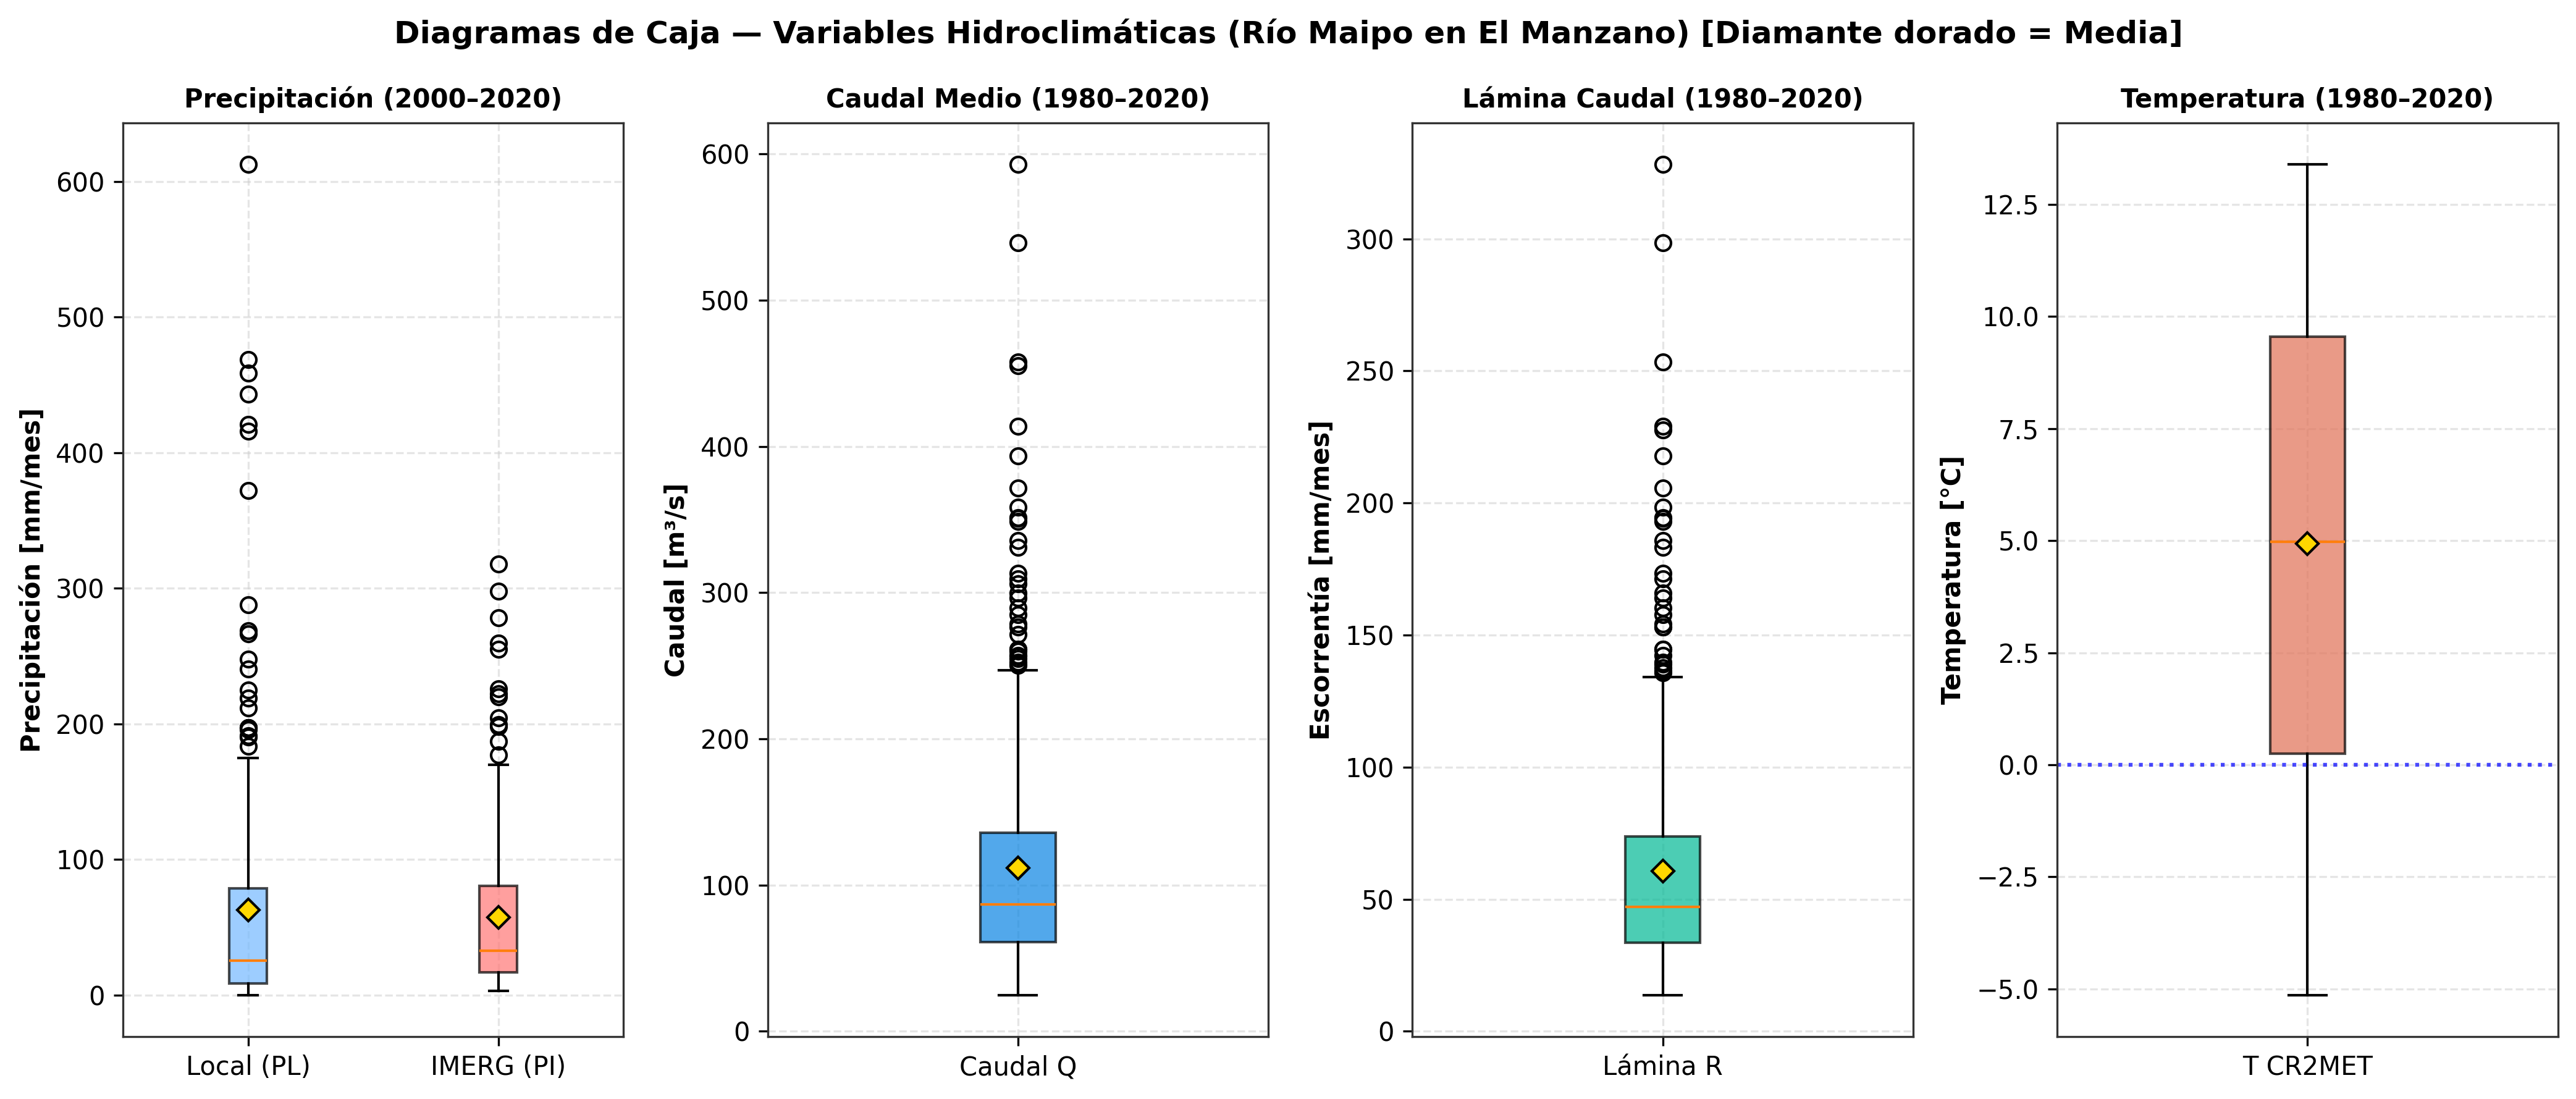
\includegraphics[width=0.95\textwidth]{figura_1_3_diagramas_caja.png}
\caption{Diagramas de caja de las variables mensuales (bigotes a 1.5 veces el rango intercuartílico; rombo: media). Los puntos fuera de los bigotes se revisaron contra el contexto y no se eliminaron.}
\label{fig:cajas}
\end{figure}

\begin{figure}[H]
\centering
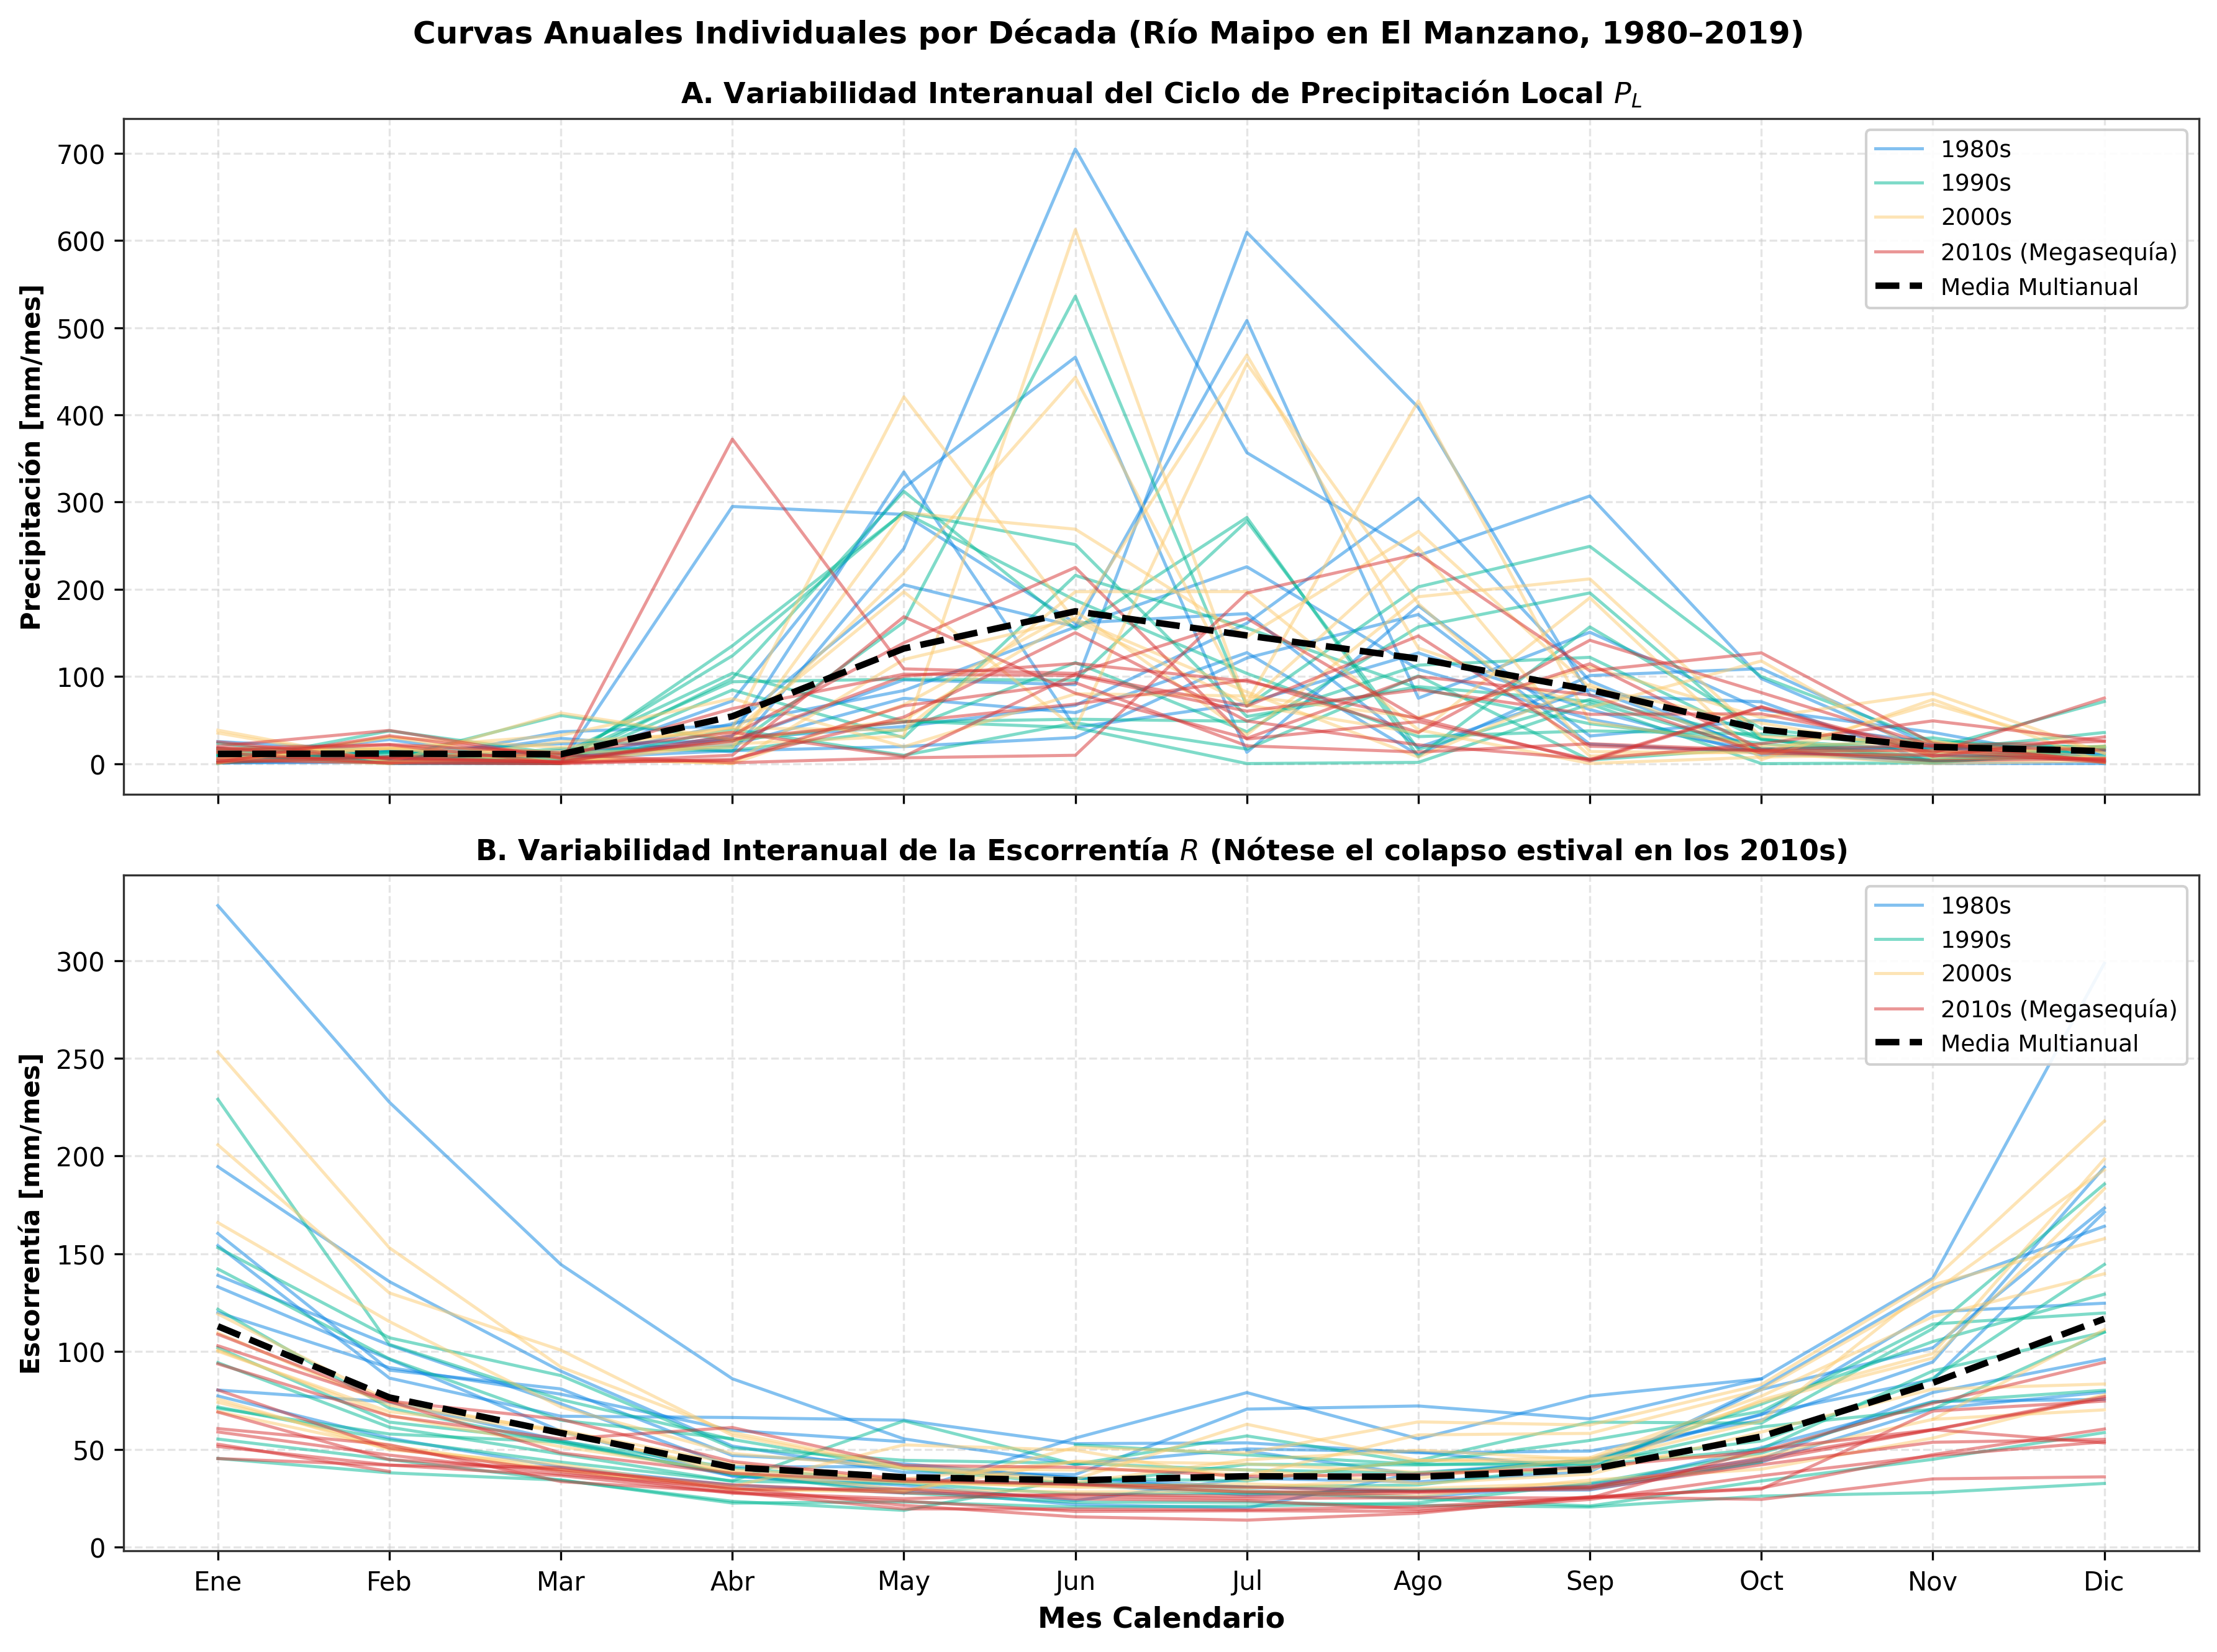
\includegraphics[width=0.9\textwidth]{figura_1_6_curvas_anuales_individuales.png}
\caption{Curvas anuales individuales, que conservan la información de cada año. Script \archivo{07_rol_a_explorador.py}.}
\label{fig:curvas}
\end{figure}

\begin{figure}[H]
\centering
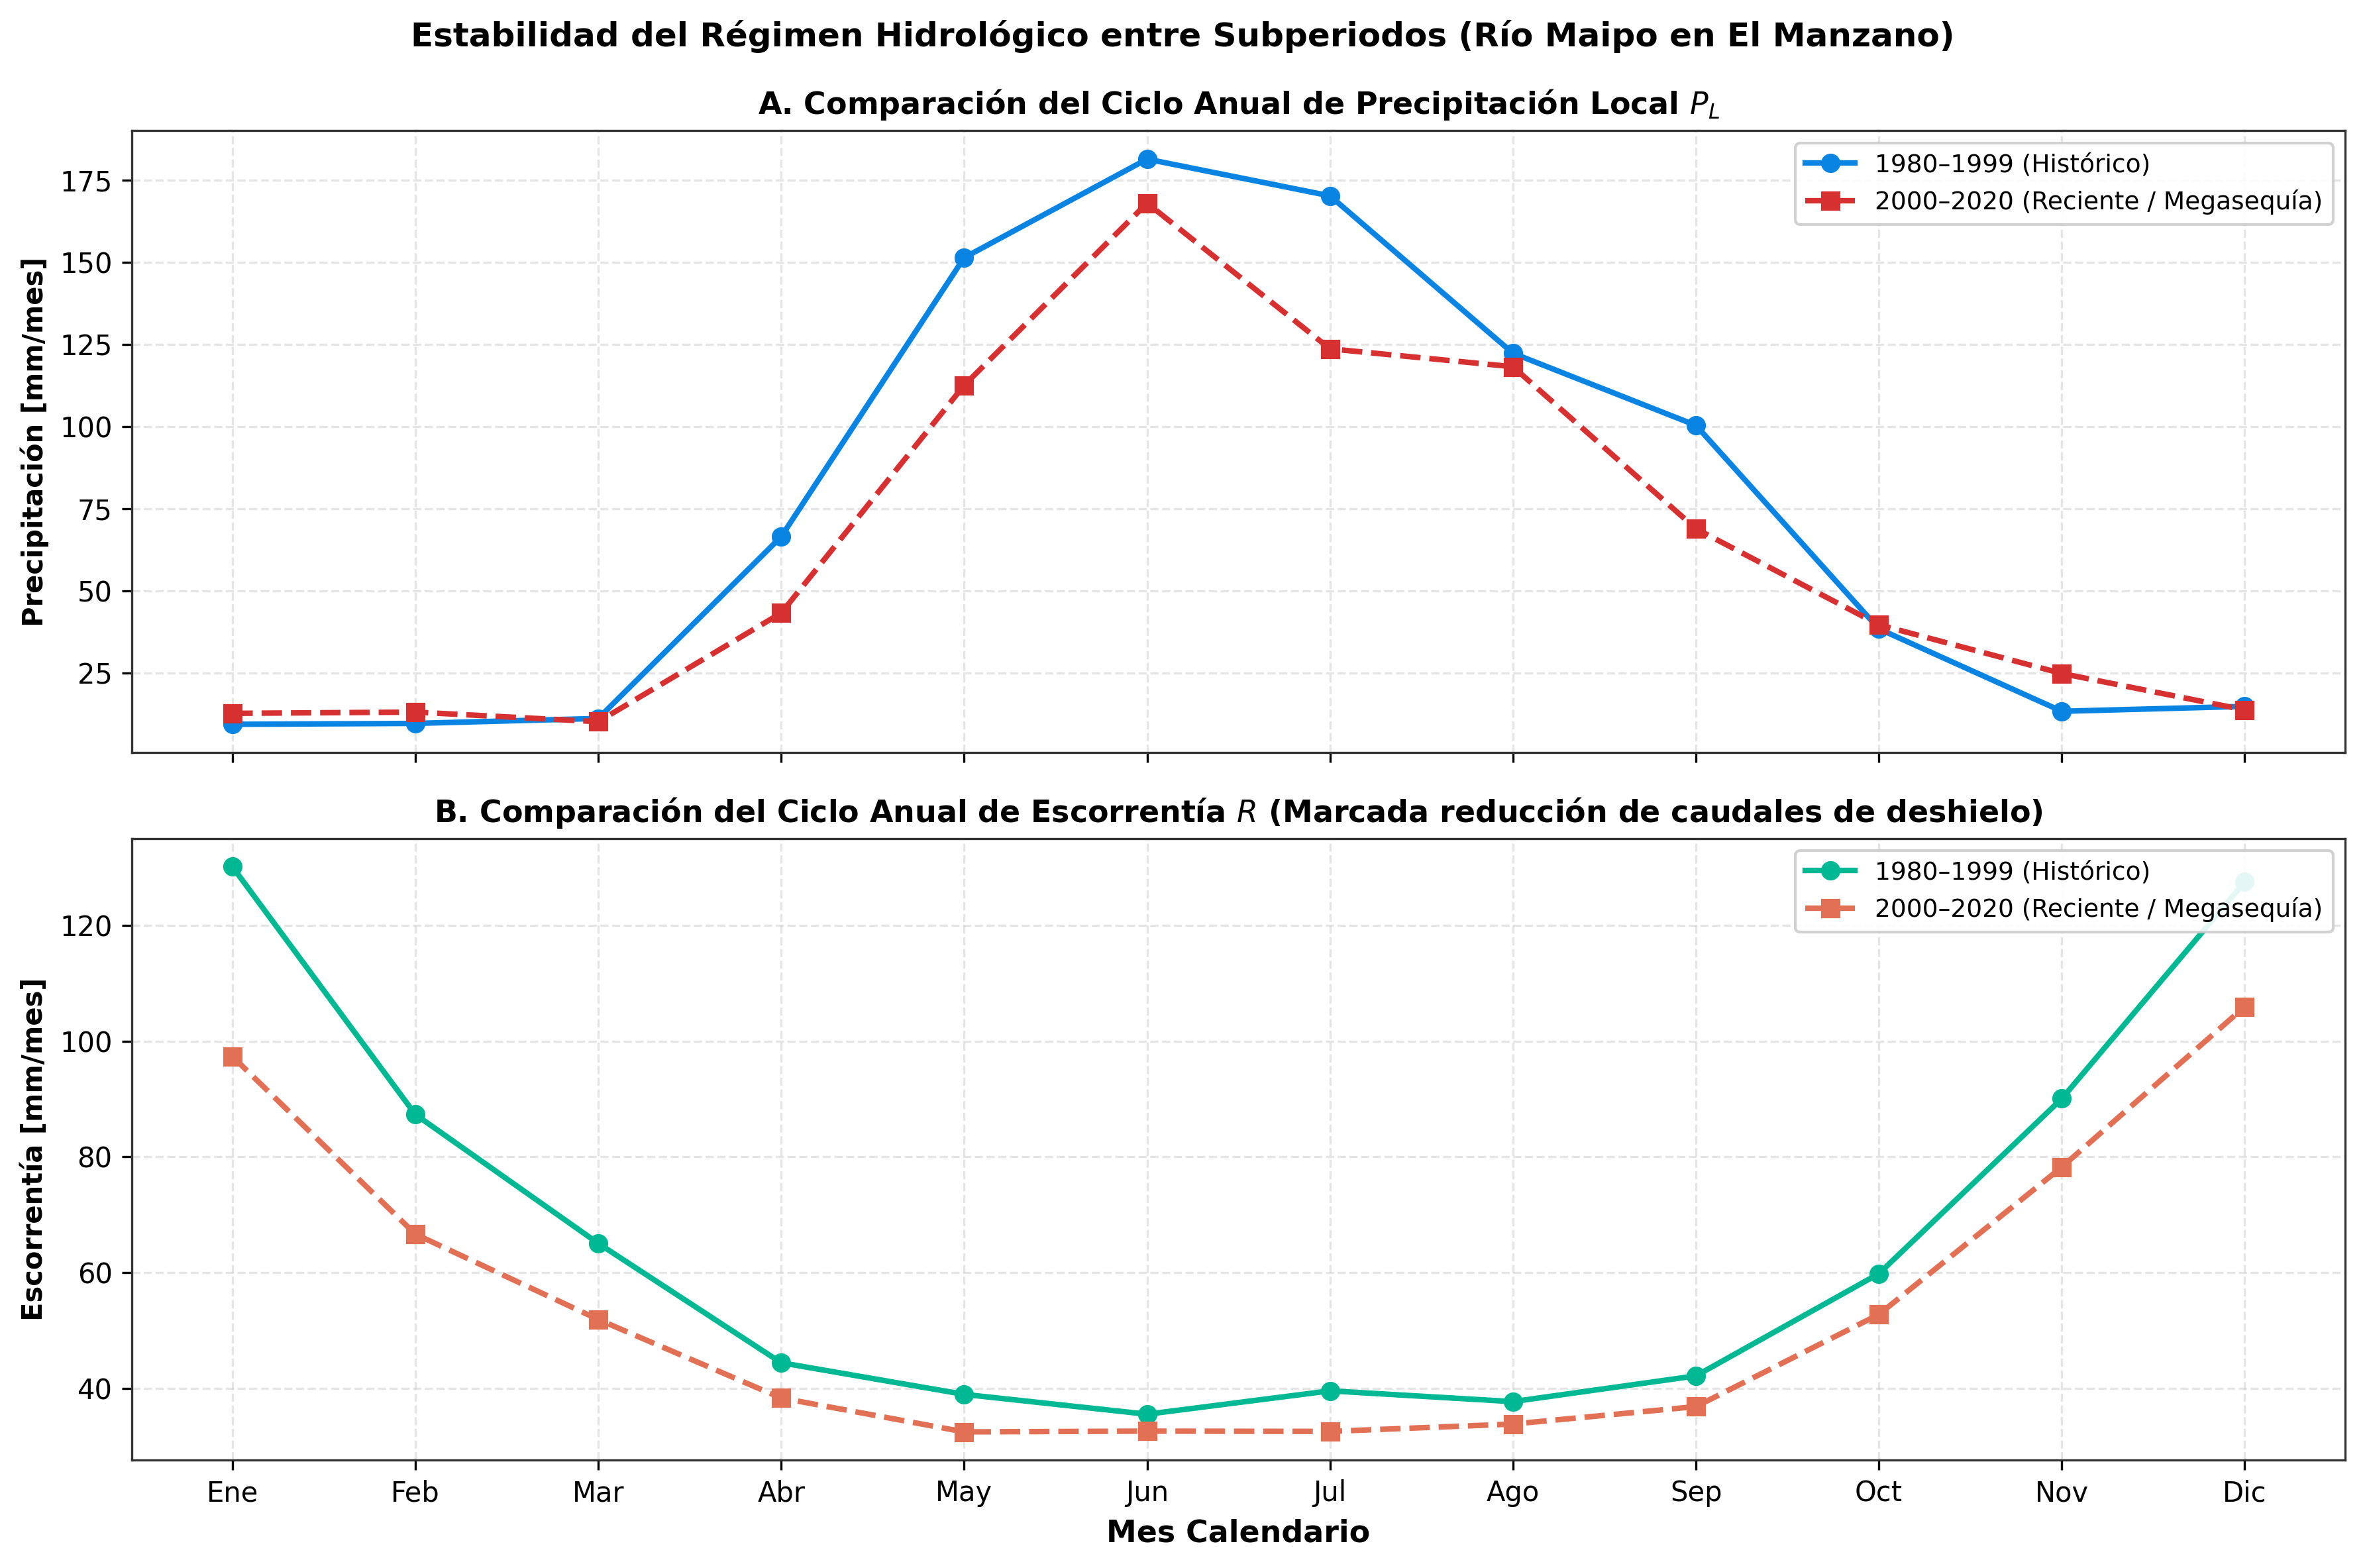
\includegraphics[width=0.9\textwidth]{figura_1_7_estabilidad_subperiodos.png}
\caption{Ciclo anual de $\PL$ y $R$ en dos subperiodos, 1980--1999 y 2000--2020 (\archivo{figuras/tabla_1_5_subperiodos_estabilidad.csv}).}
\label{fig:subper}
\end{figure}

\begin{figure}[H]
\centering
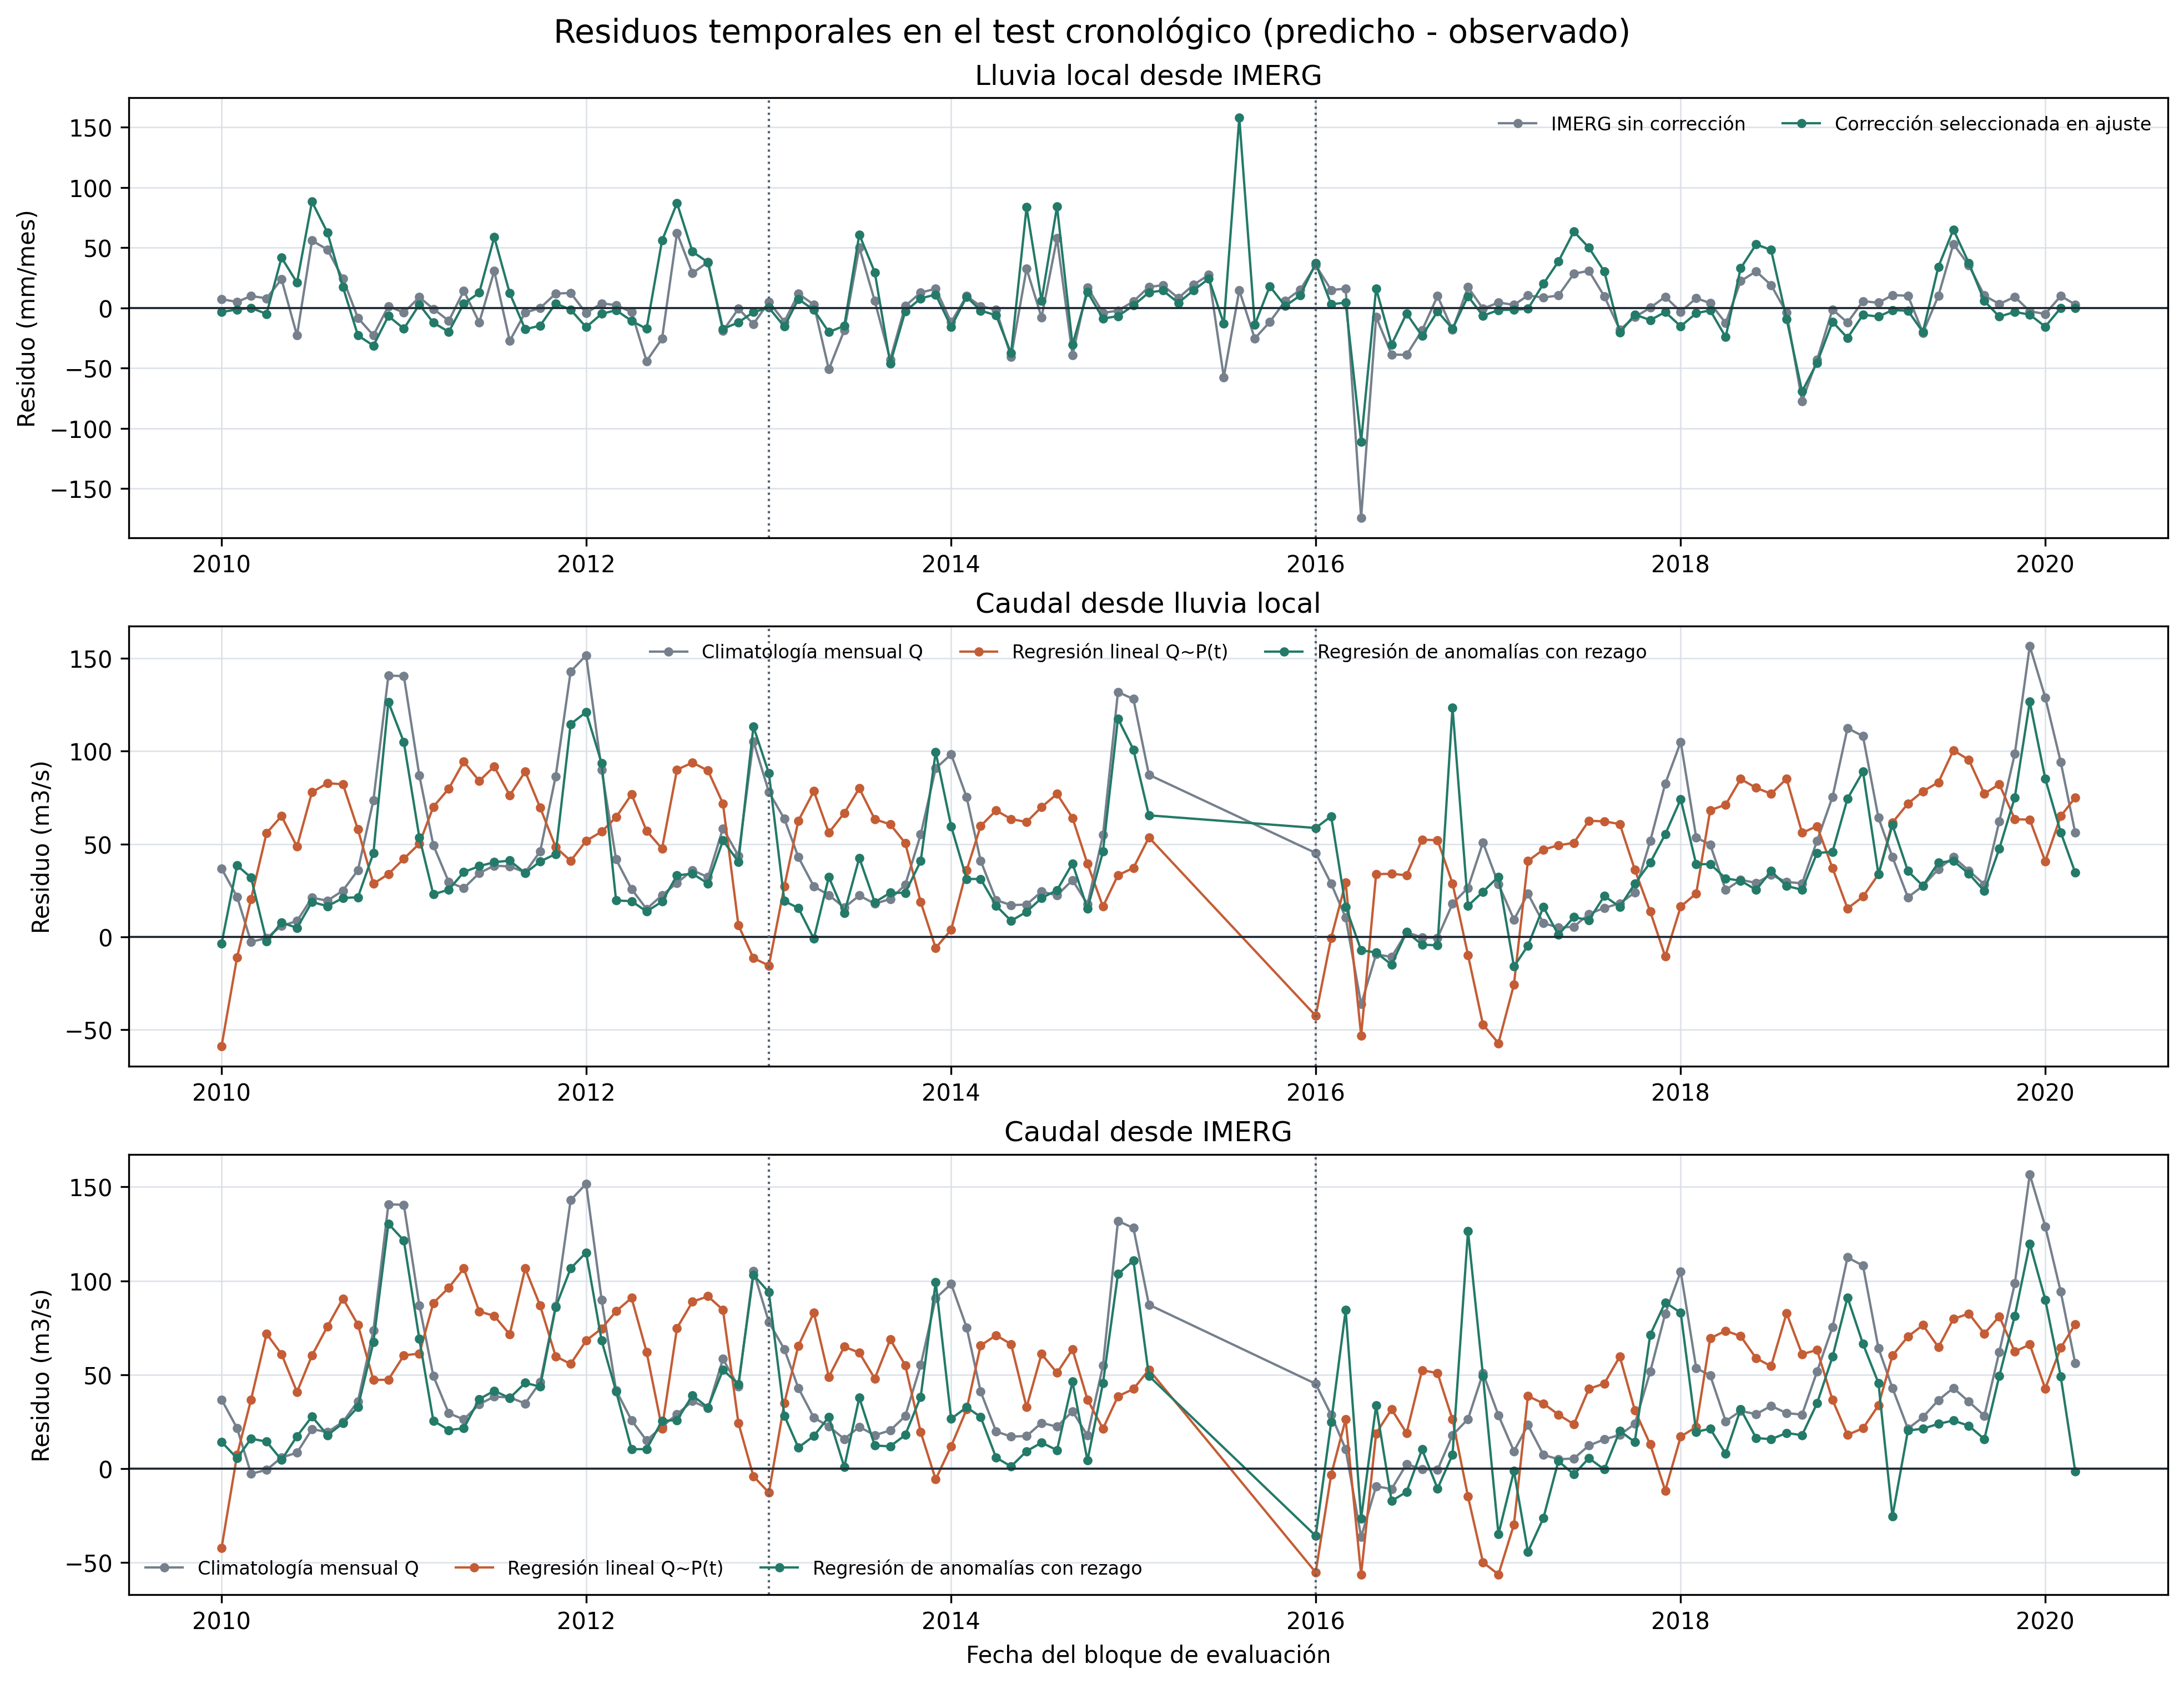
\includegraphics[width=0.92\textwidth]{figura_2_4_residuos_en_tiempo.png}
\caption{Residuos (predicción $-$ observado) en el tiempo durante la evaluación cronológica. Los residuos por mes calendario, año y estación están en \archivo{figuras/tabla_2_3_residuos_por_mes.csv}, \archivo{tabla_2_3_metricas_por_anio.csv} y \archivo{tabla_2_3_metricas_por_estacion.csv}.}
\label{fig:residuos2}
\end{figure}

\begin{figure}[H]
\centering
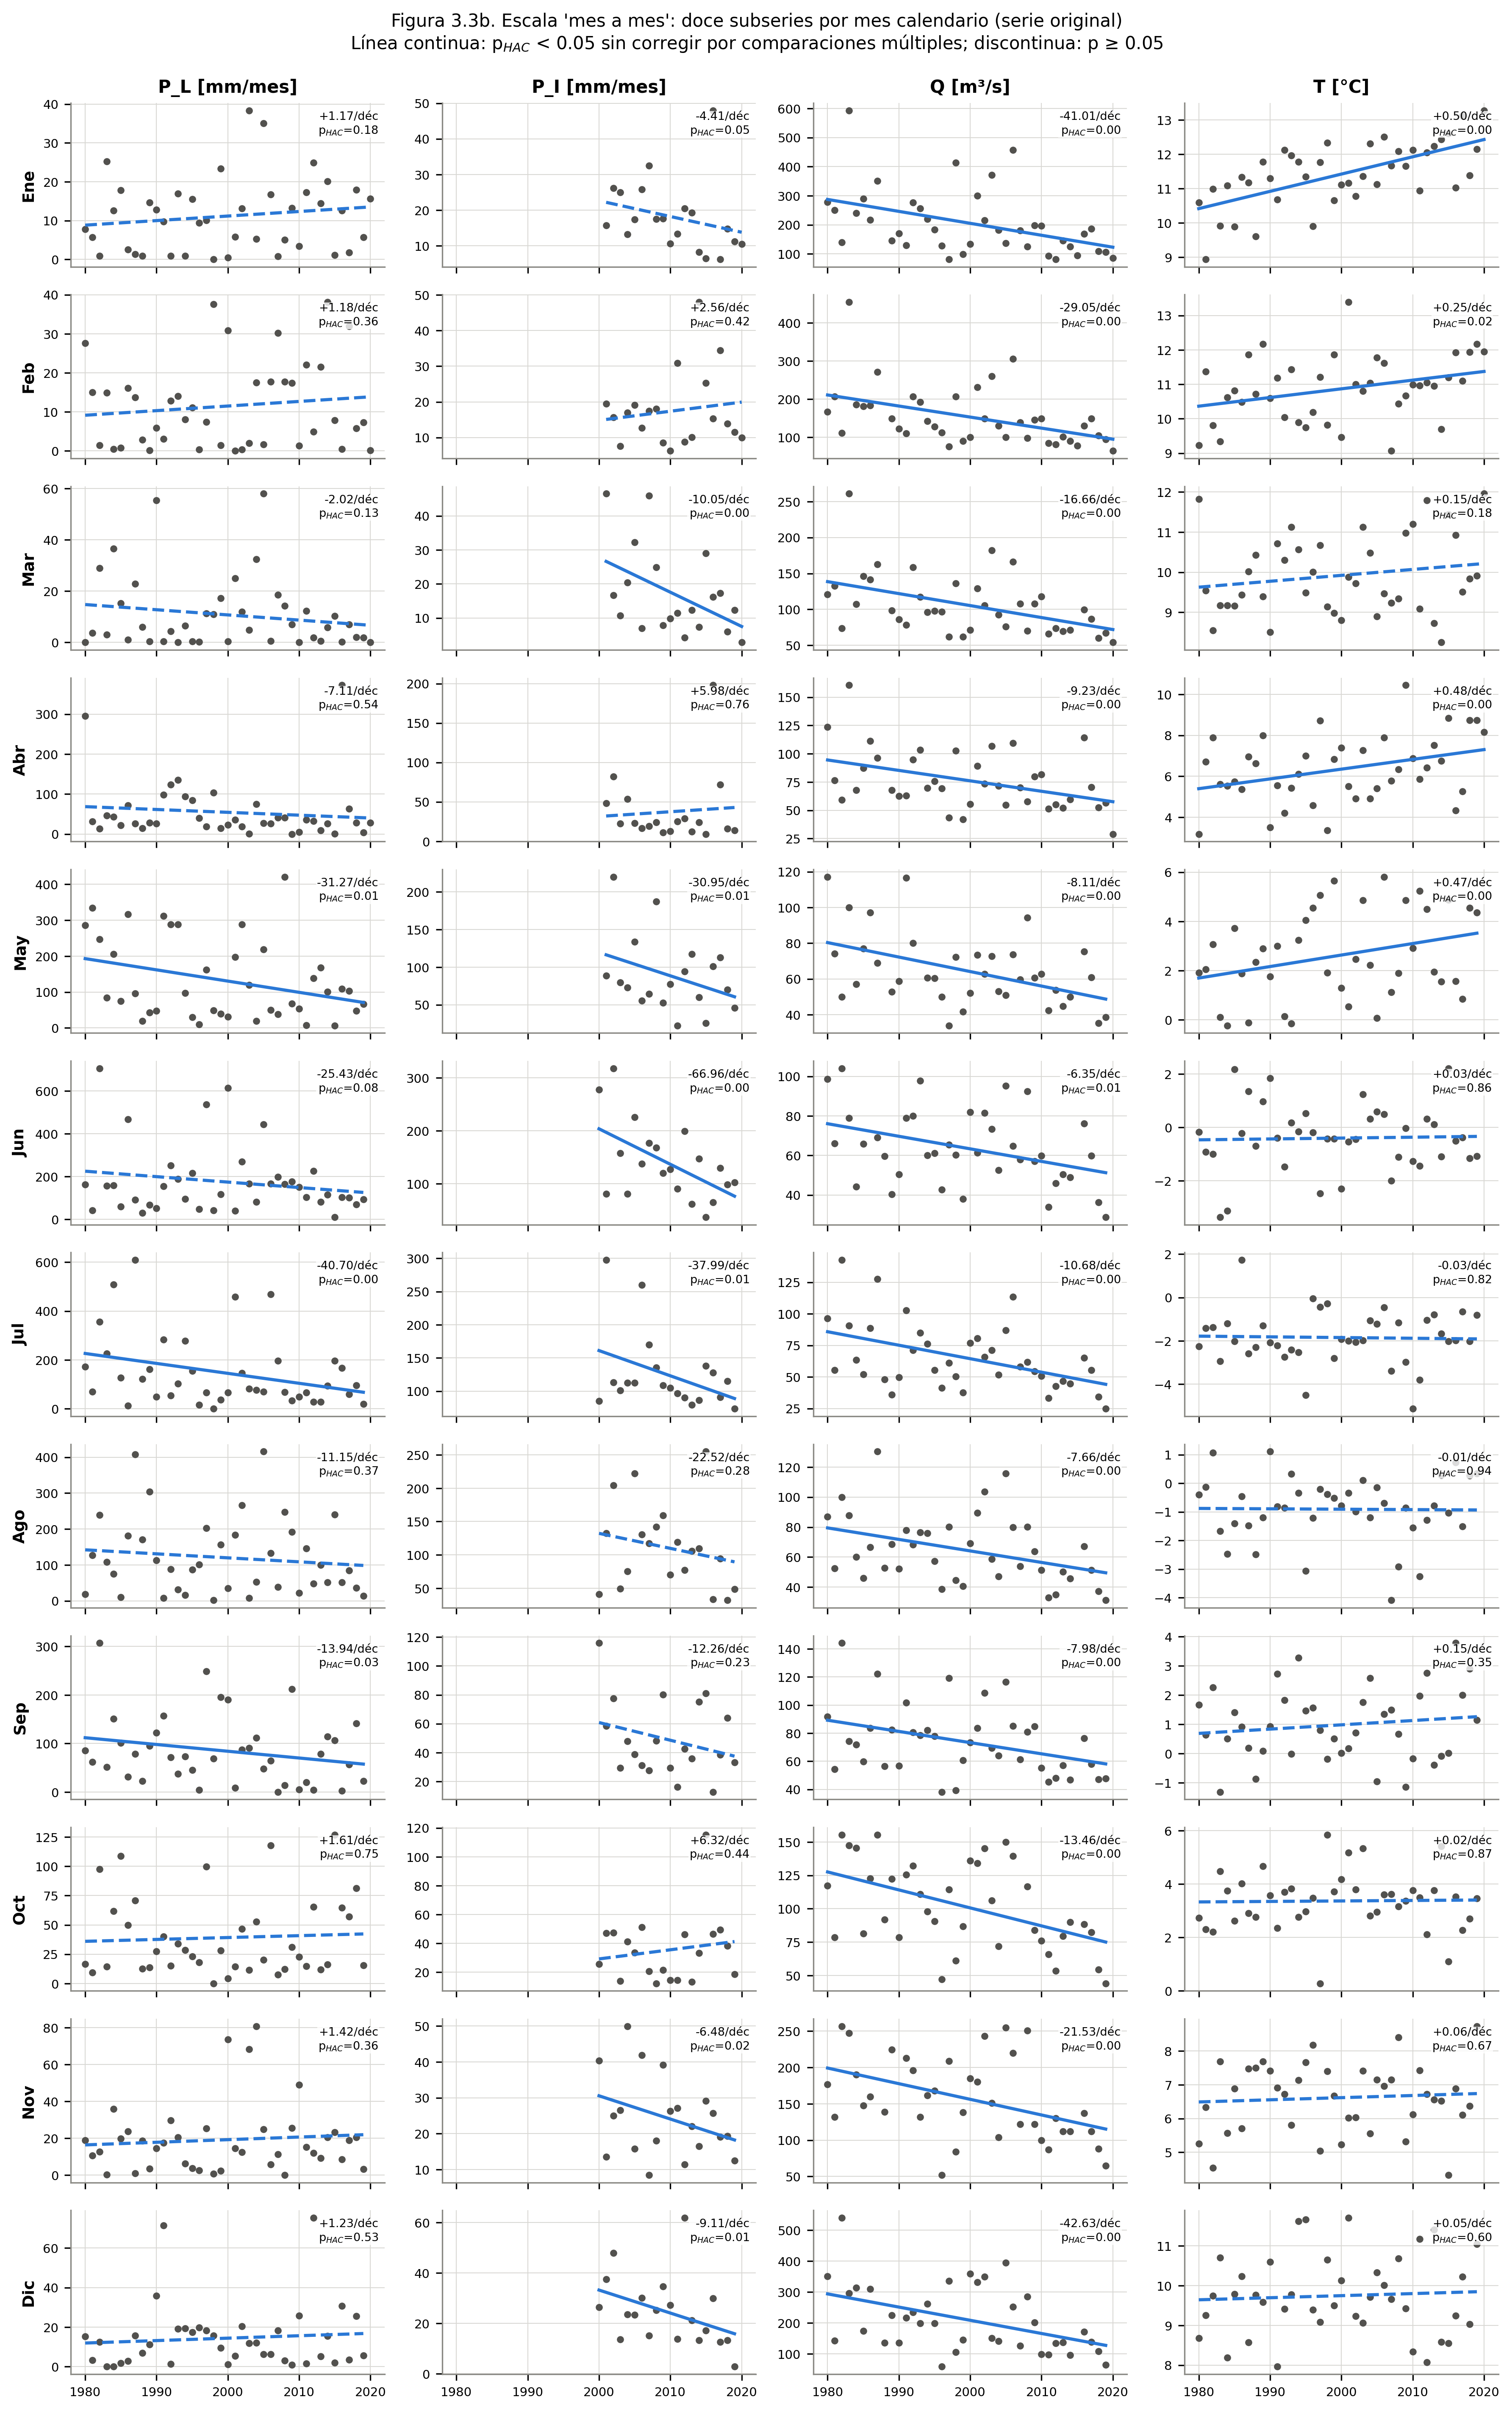
\includegraphics[height=0.70\textheight,keepaspectratio]{figura_3_3b_subseries_mensuales.png}
\caption{Escala ``mes a mes'': doce subseries por mes calendario (serie original) con su recta OLS. Línea continua: $p_{\mathrm{HAC}}<0.05$ antes de corregir por comparaciones múltiples.}
\label{fig:mensual}
\end{figure}

\begin{figure}[H]
\centering
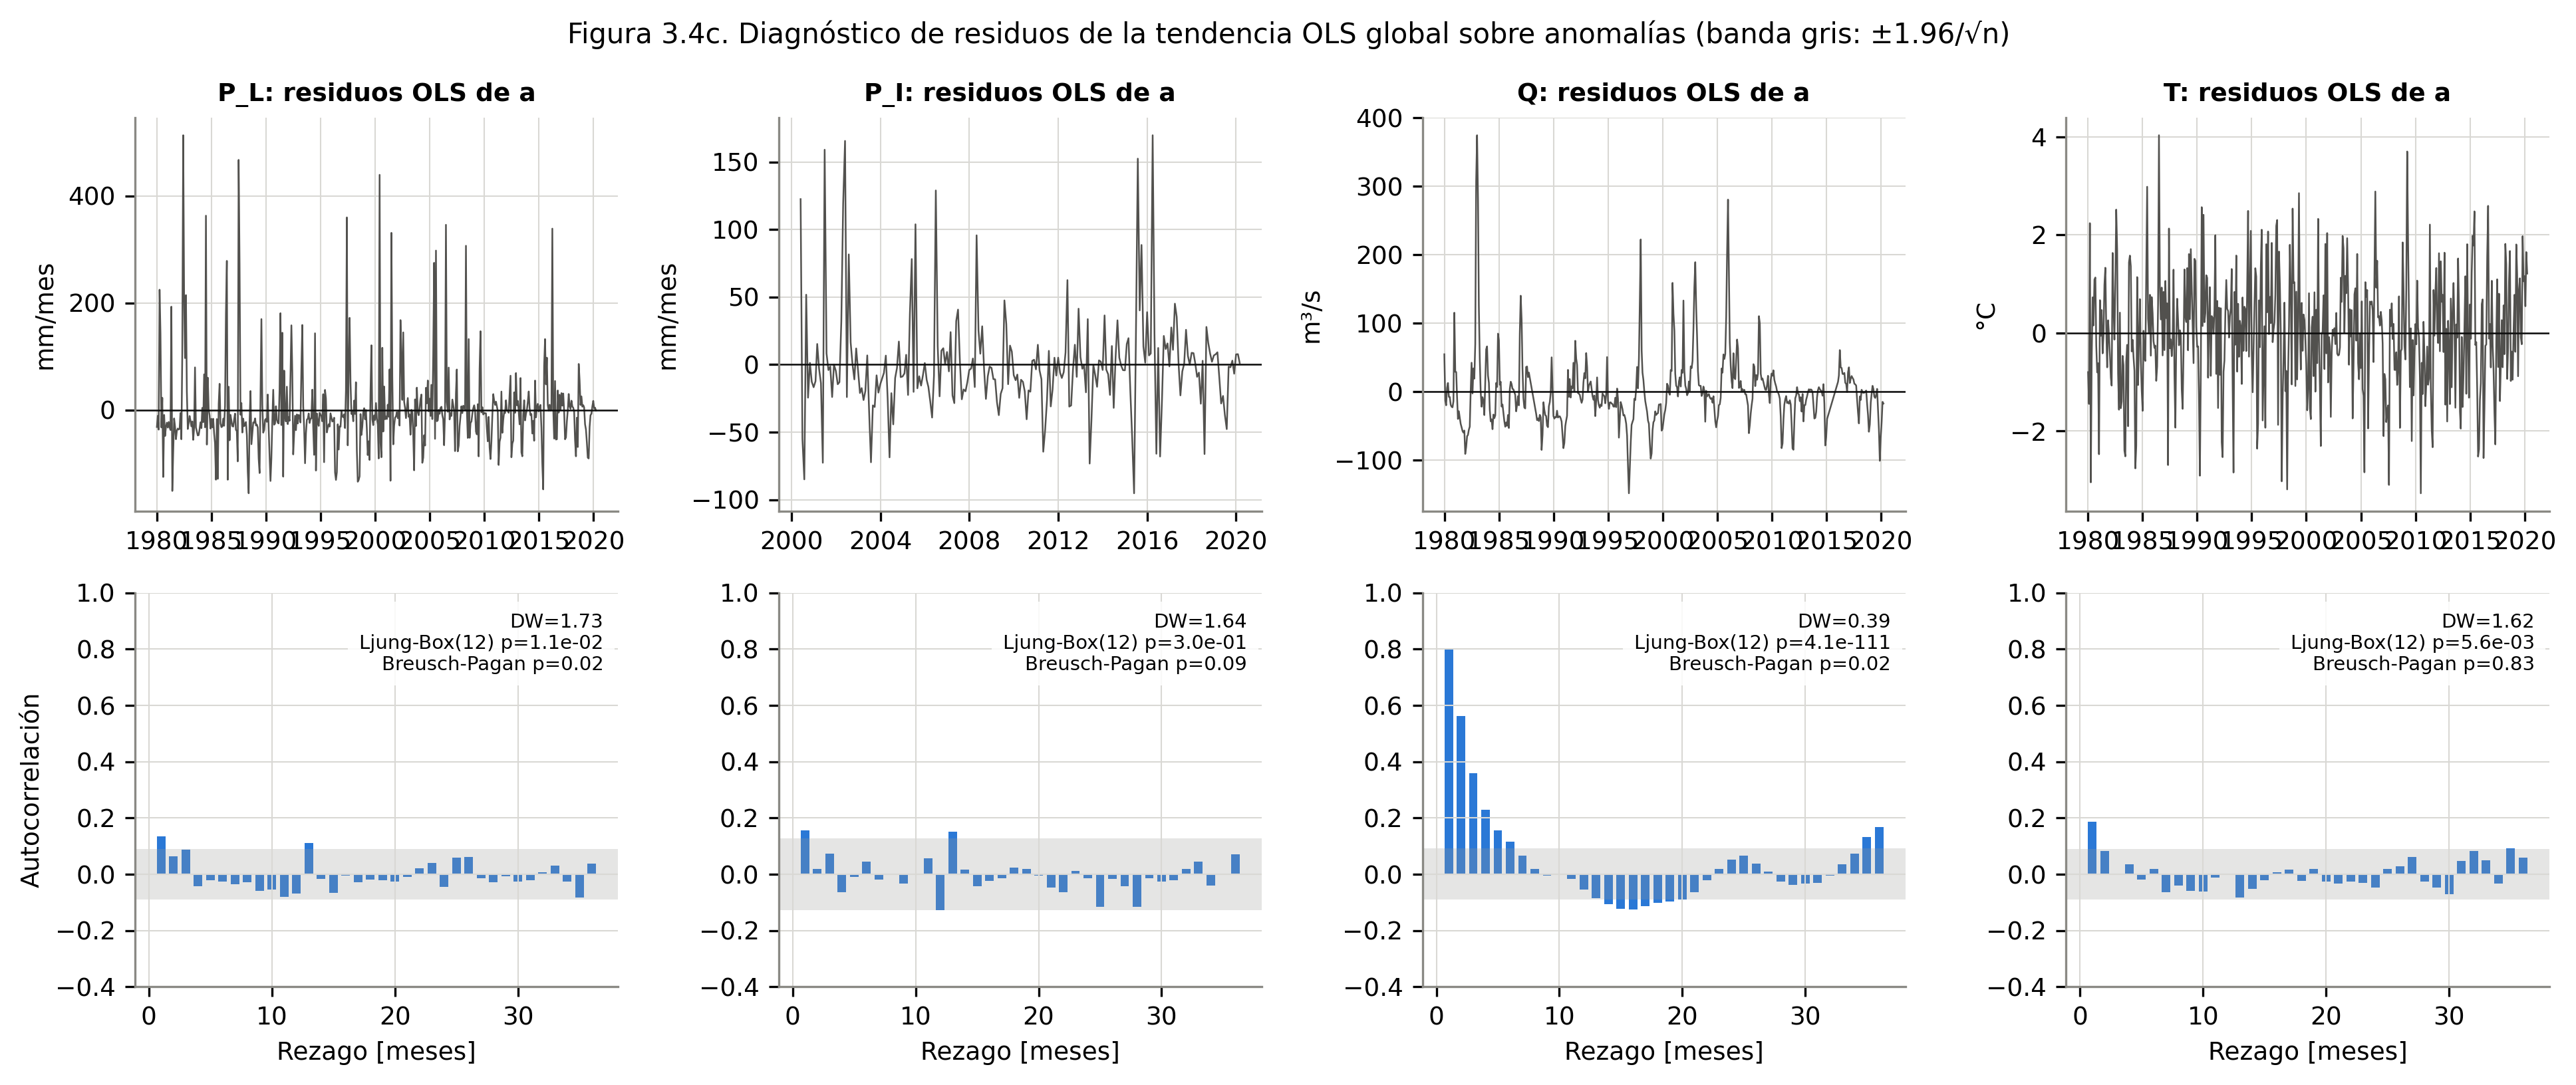
\includegraphics[width=0.95\textwidth]{figura_3_4c_diagnostico_residuos.png}
\caption{Diagnóstico de residuos de la OLS global sobre anomalías: residuos en el tiempo y autocorrelación (banda: $\pm1.96/\sqrt n$).}
\label{fig:resid}
\end{figure}

\begin{figure}[H]
\centering
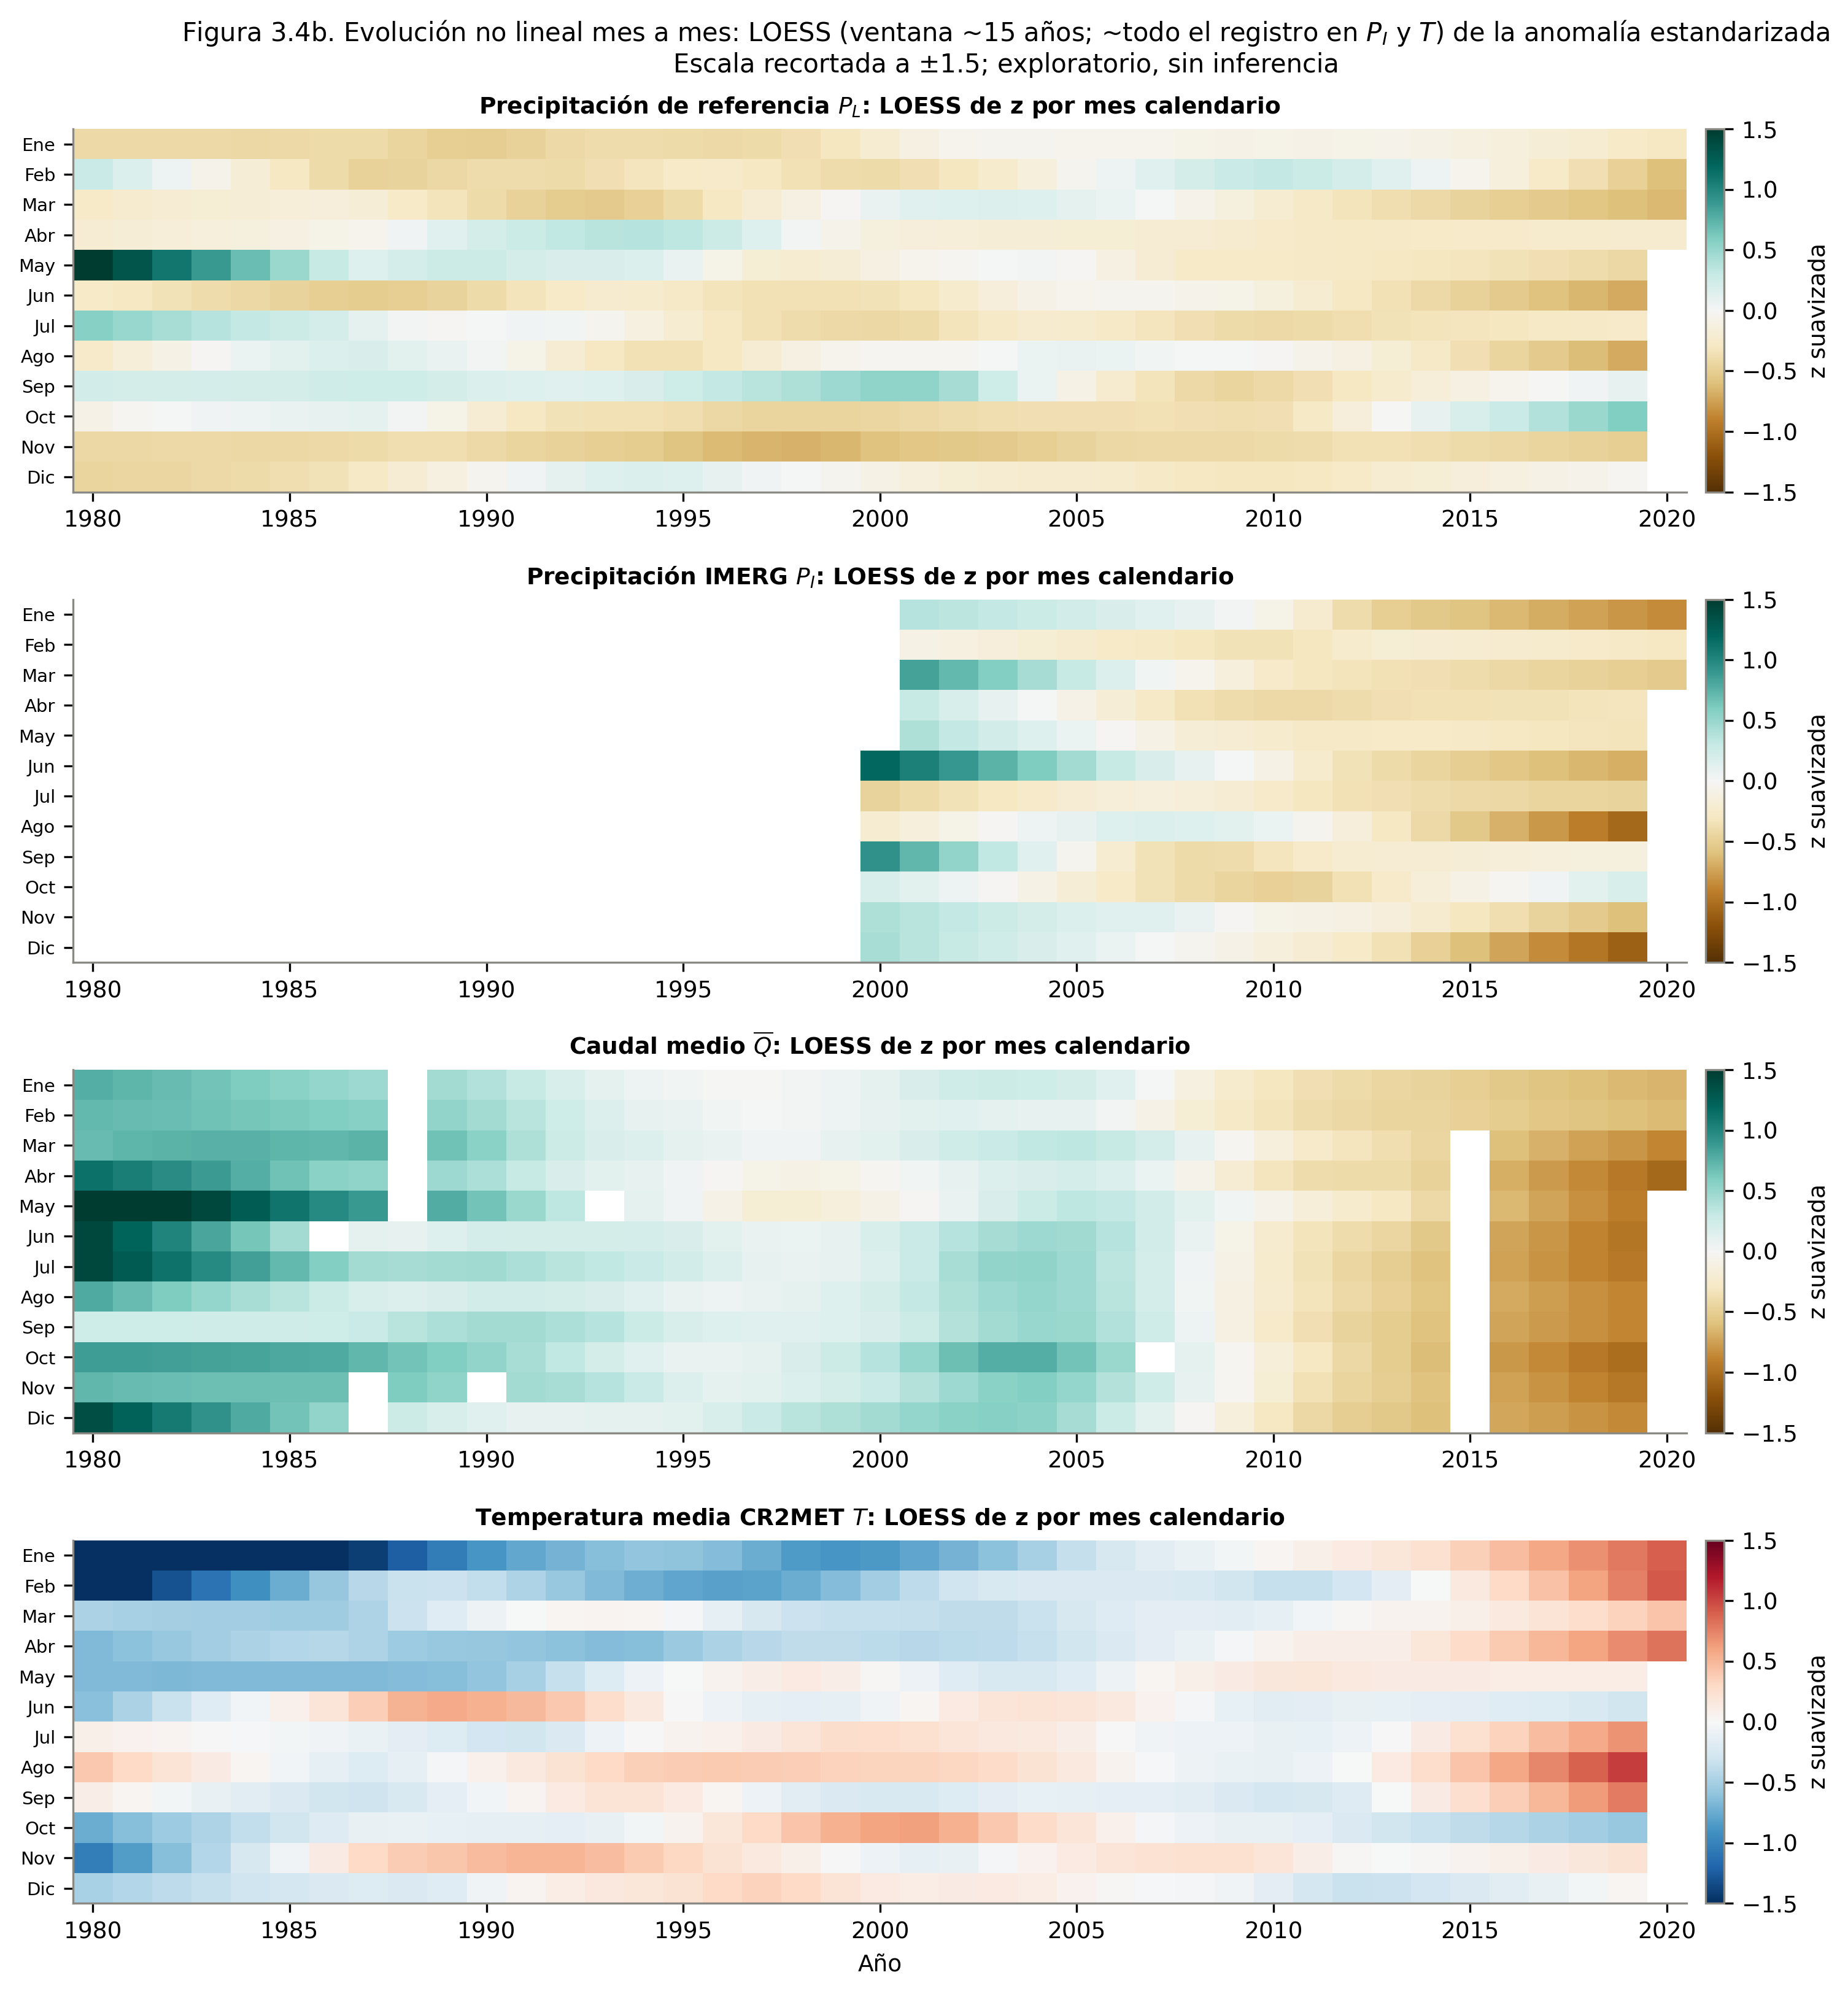
\includegraphics[width=0.75\textwidth]{figura_3_4b_loess_mes_anio.png}
\caption{LOESS de la anomalía estandarizada de cada mes calendario (mapa año--mes). Exploratorio; en $\PI$ y $T$ la ventana cubre casi todo el registro.}
\label{fig:loessmes}
\end{figure}

\begin{figure}[H]
\centering
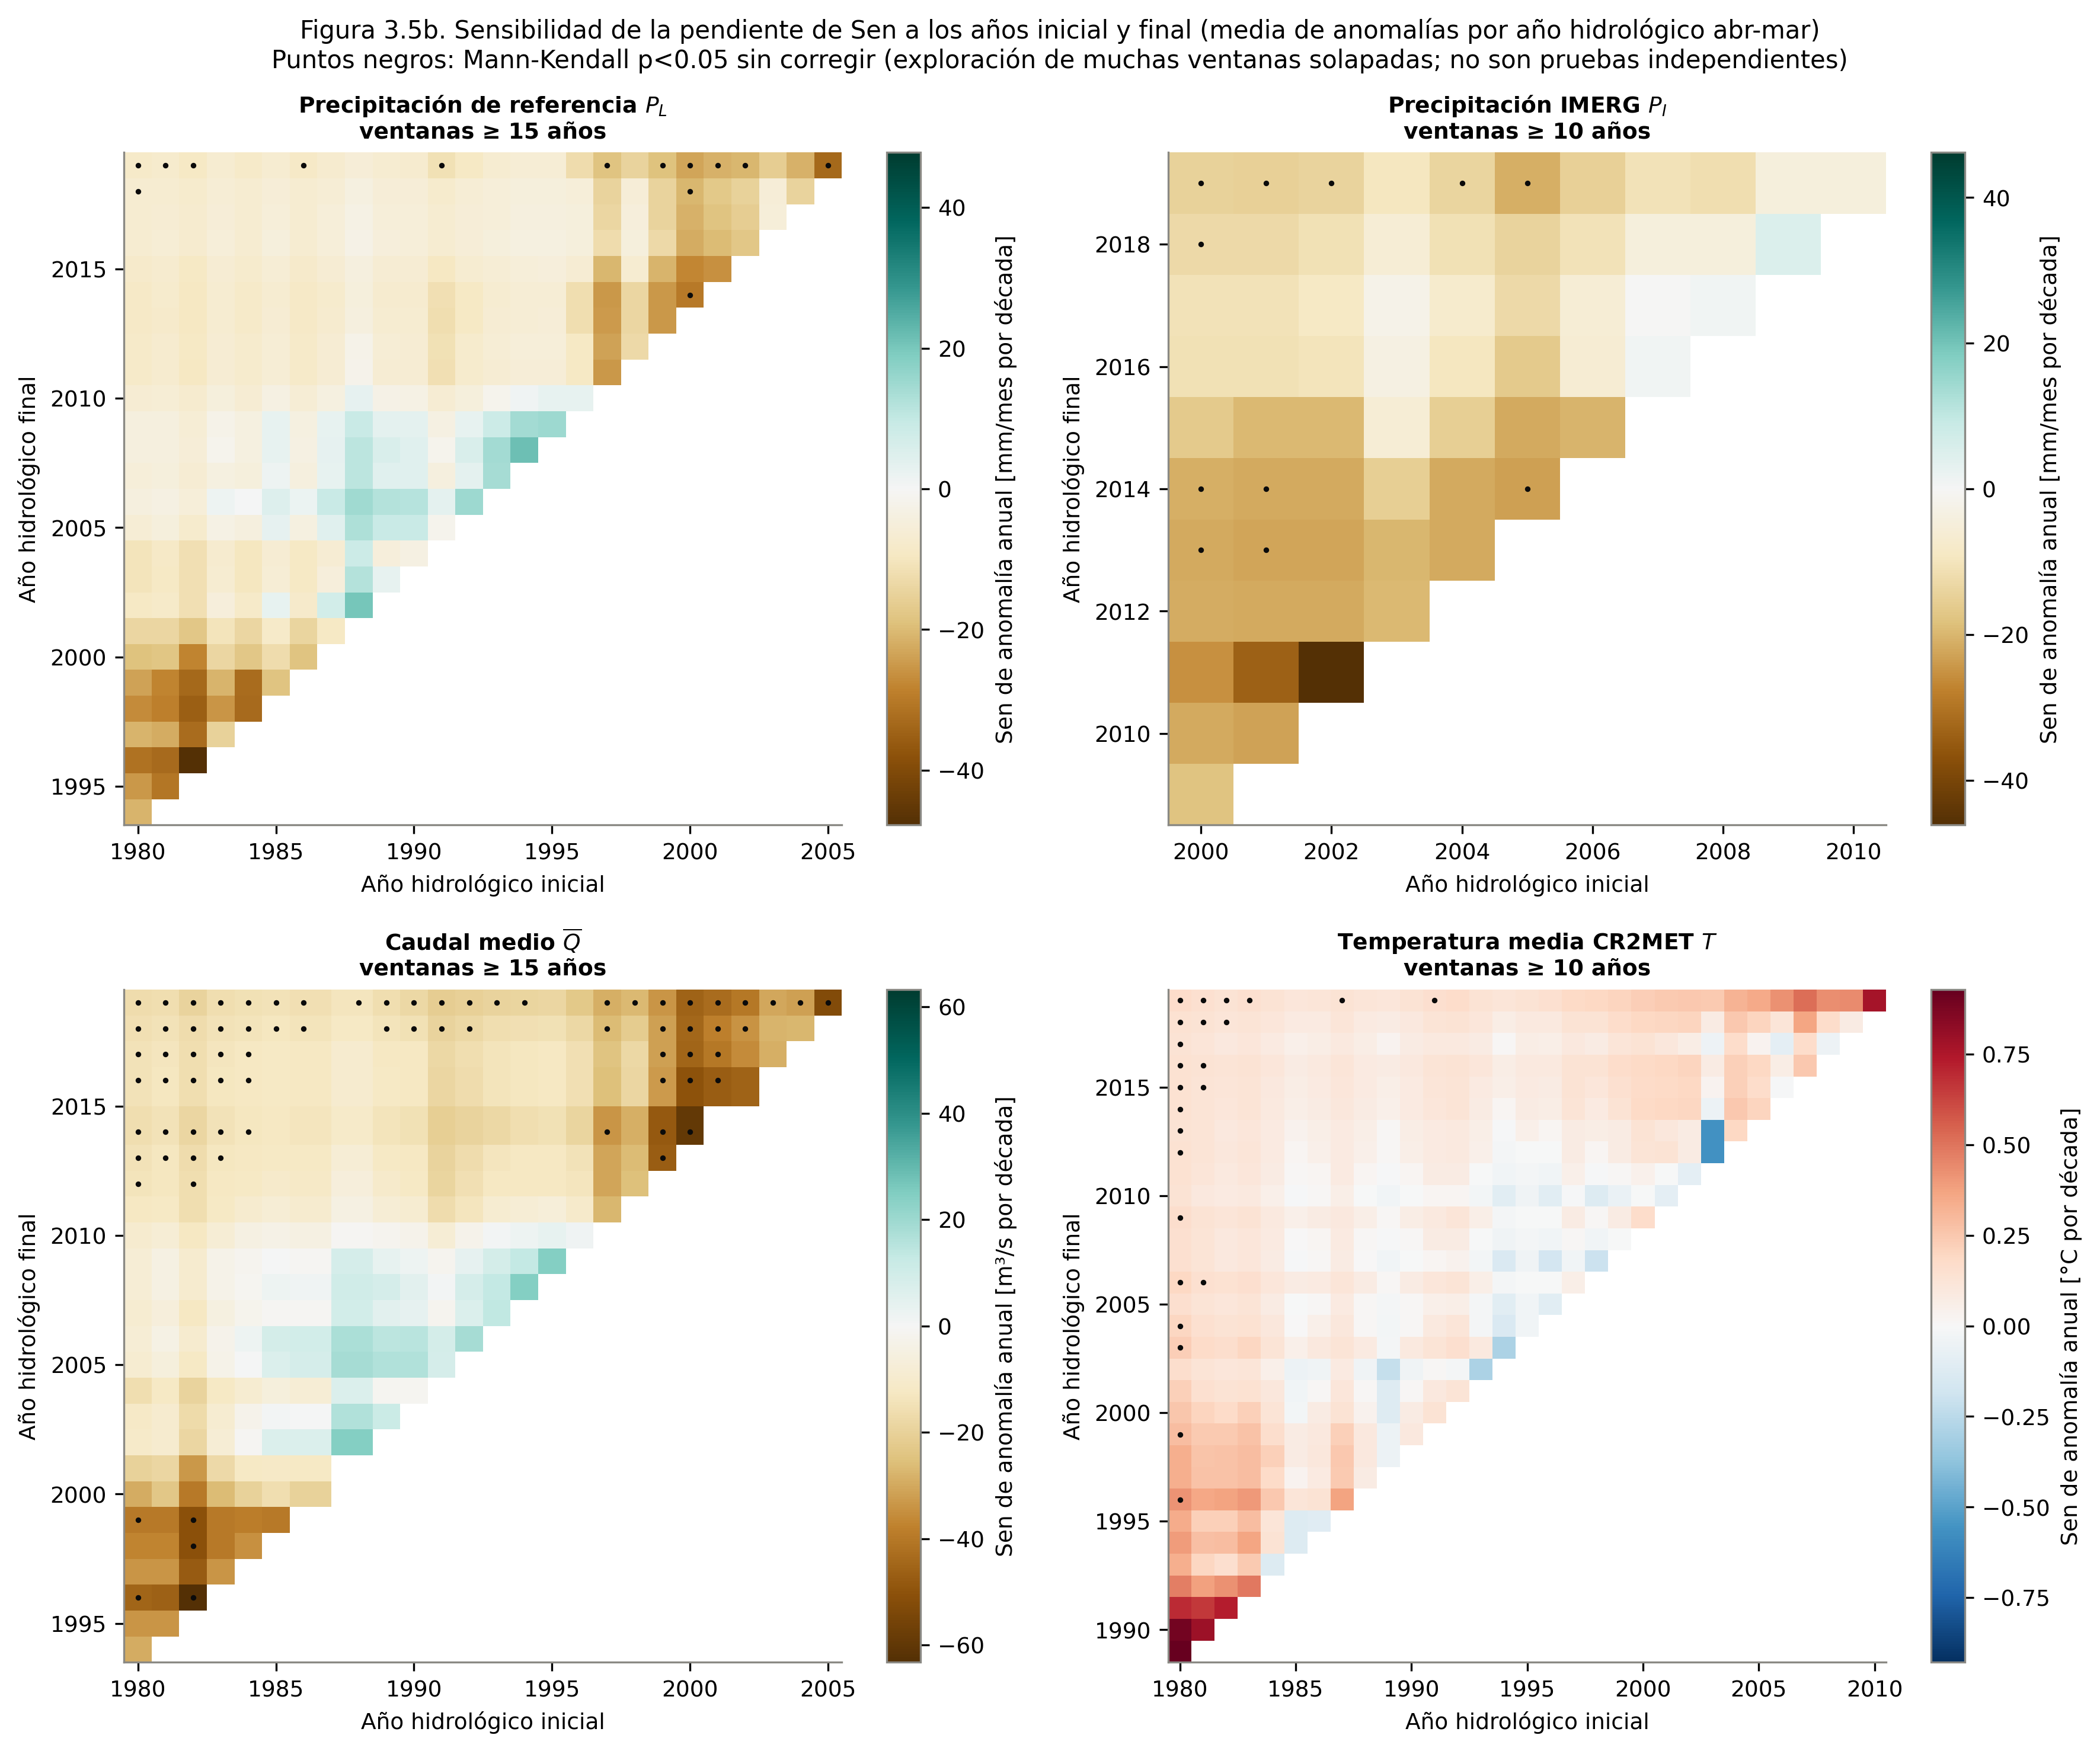
\includegraphics[width=0.9\textwidth]{figura_3_5b_sensibilidad_inicio_fin.png}
\caption{Pendiente de Sen de la anomalía media por año hidrológico (abril--marzo) para todas las ventanas de al menos 15 años ($\PL$, $\Qm$) o 10 años ($\PI$, $T$). Puntos: Mann--Kendall $p<0.05$ sin corregir; son ventanas solapadas, no pruebas independientes.}
\label{fig:inifin}
\end{figure}

\begin{figure}[H]
\centering
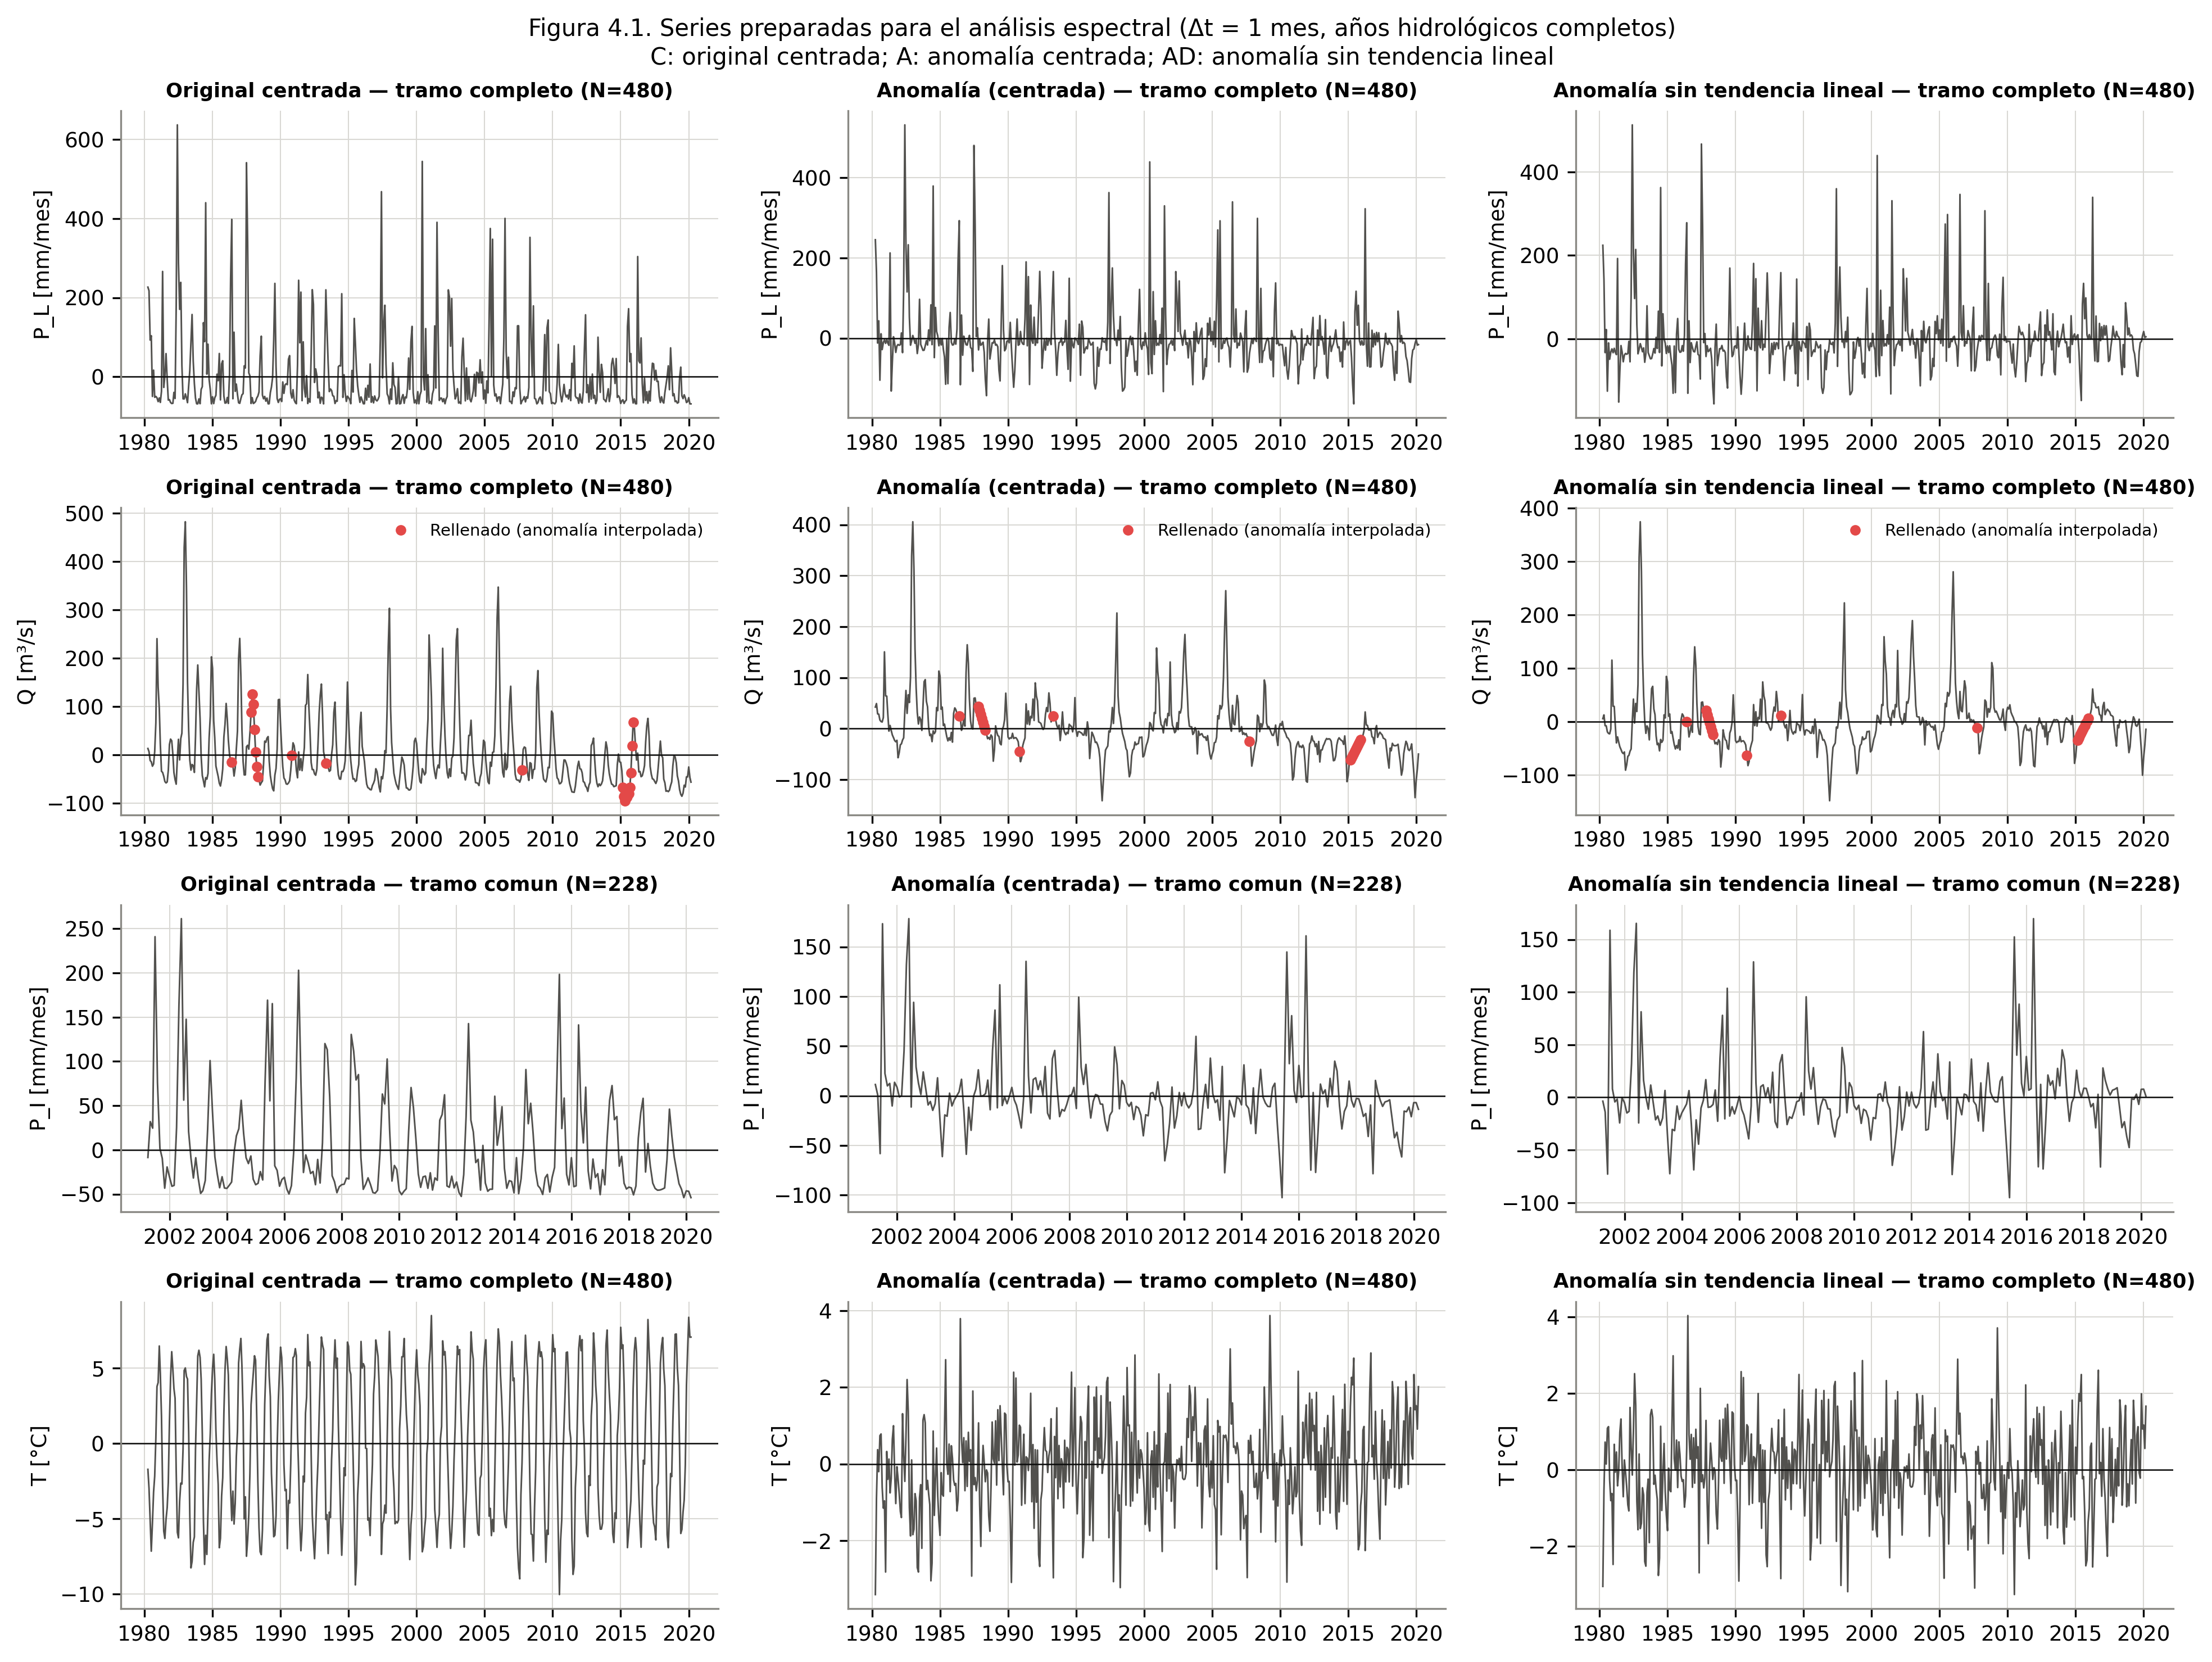
\includegraphics[width=0.9\textwidth]{figura_4_1_series_preparadas.png}
\caption{Series preparadas para el análisis espectral: serie centrada (C), anomalía (A) y anomalía sin tendencia (AD). Puntos rojos: meses de caudal rellenados interpolando la anomalía. Script \archivo{13_p4_1_preparacion_espectral.py}.}
\label{fig:prep}
\end{figure}

\begin{figure}[H]
\centering
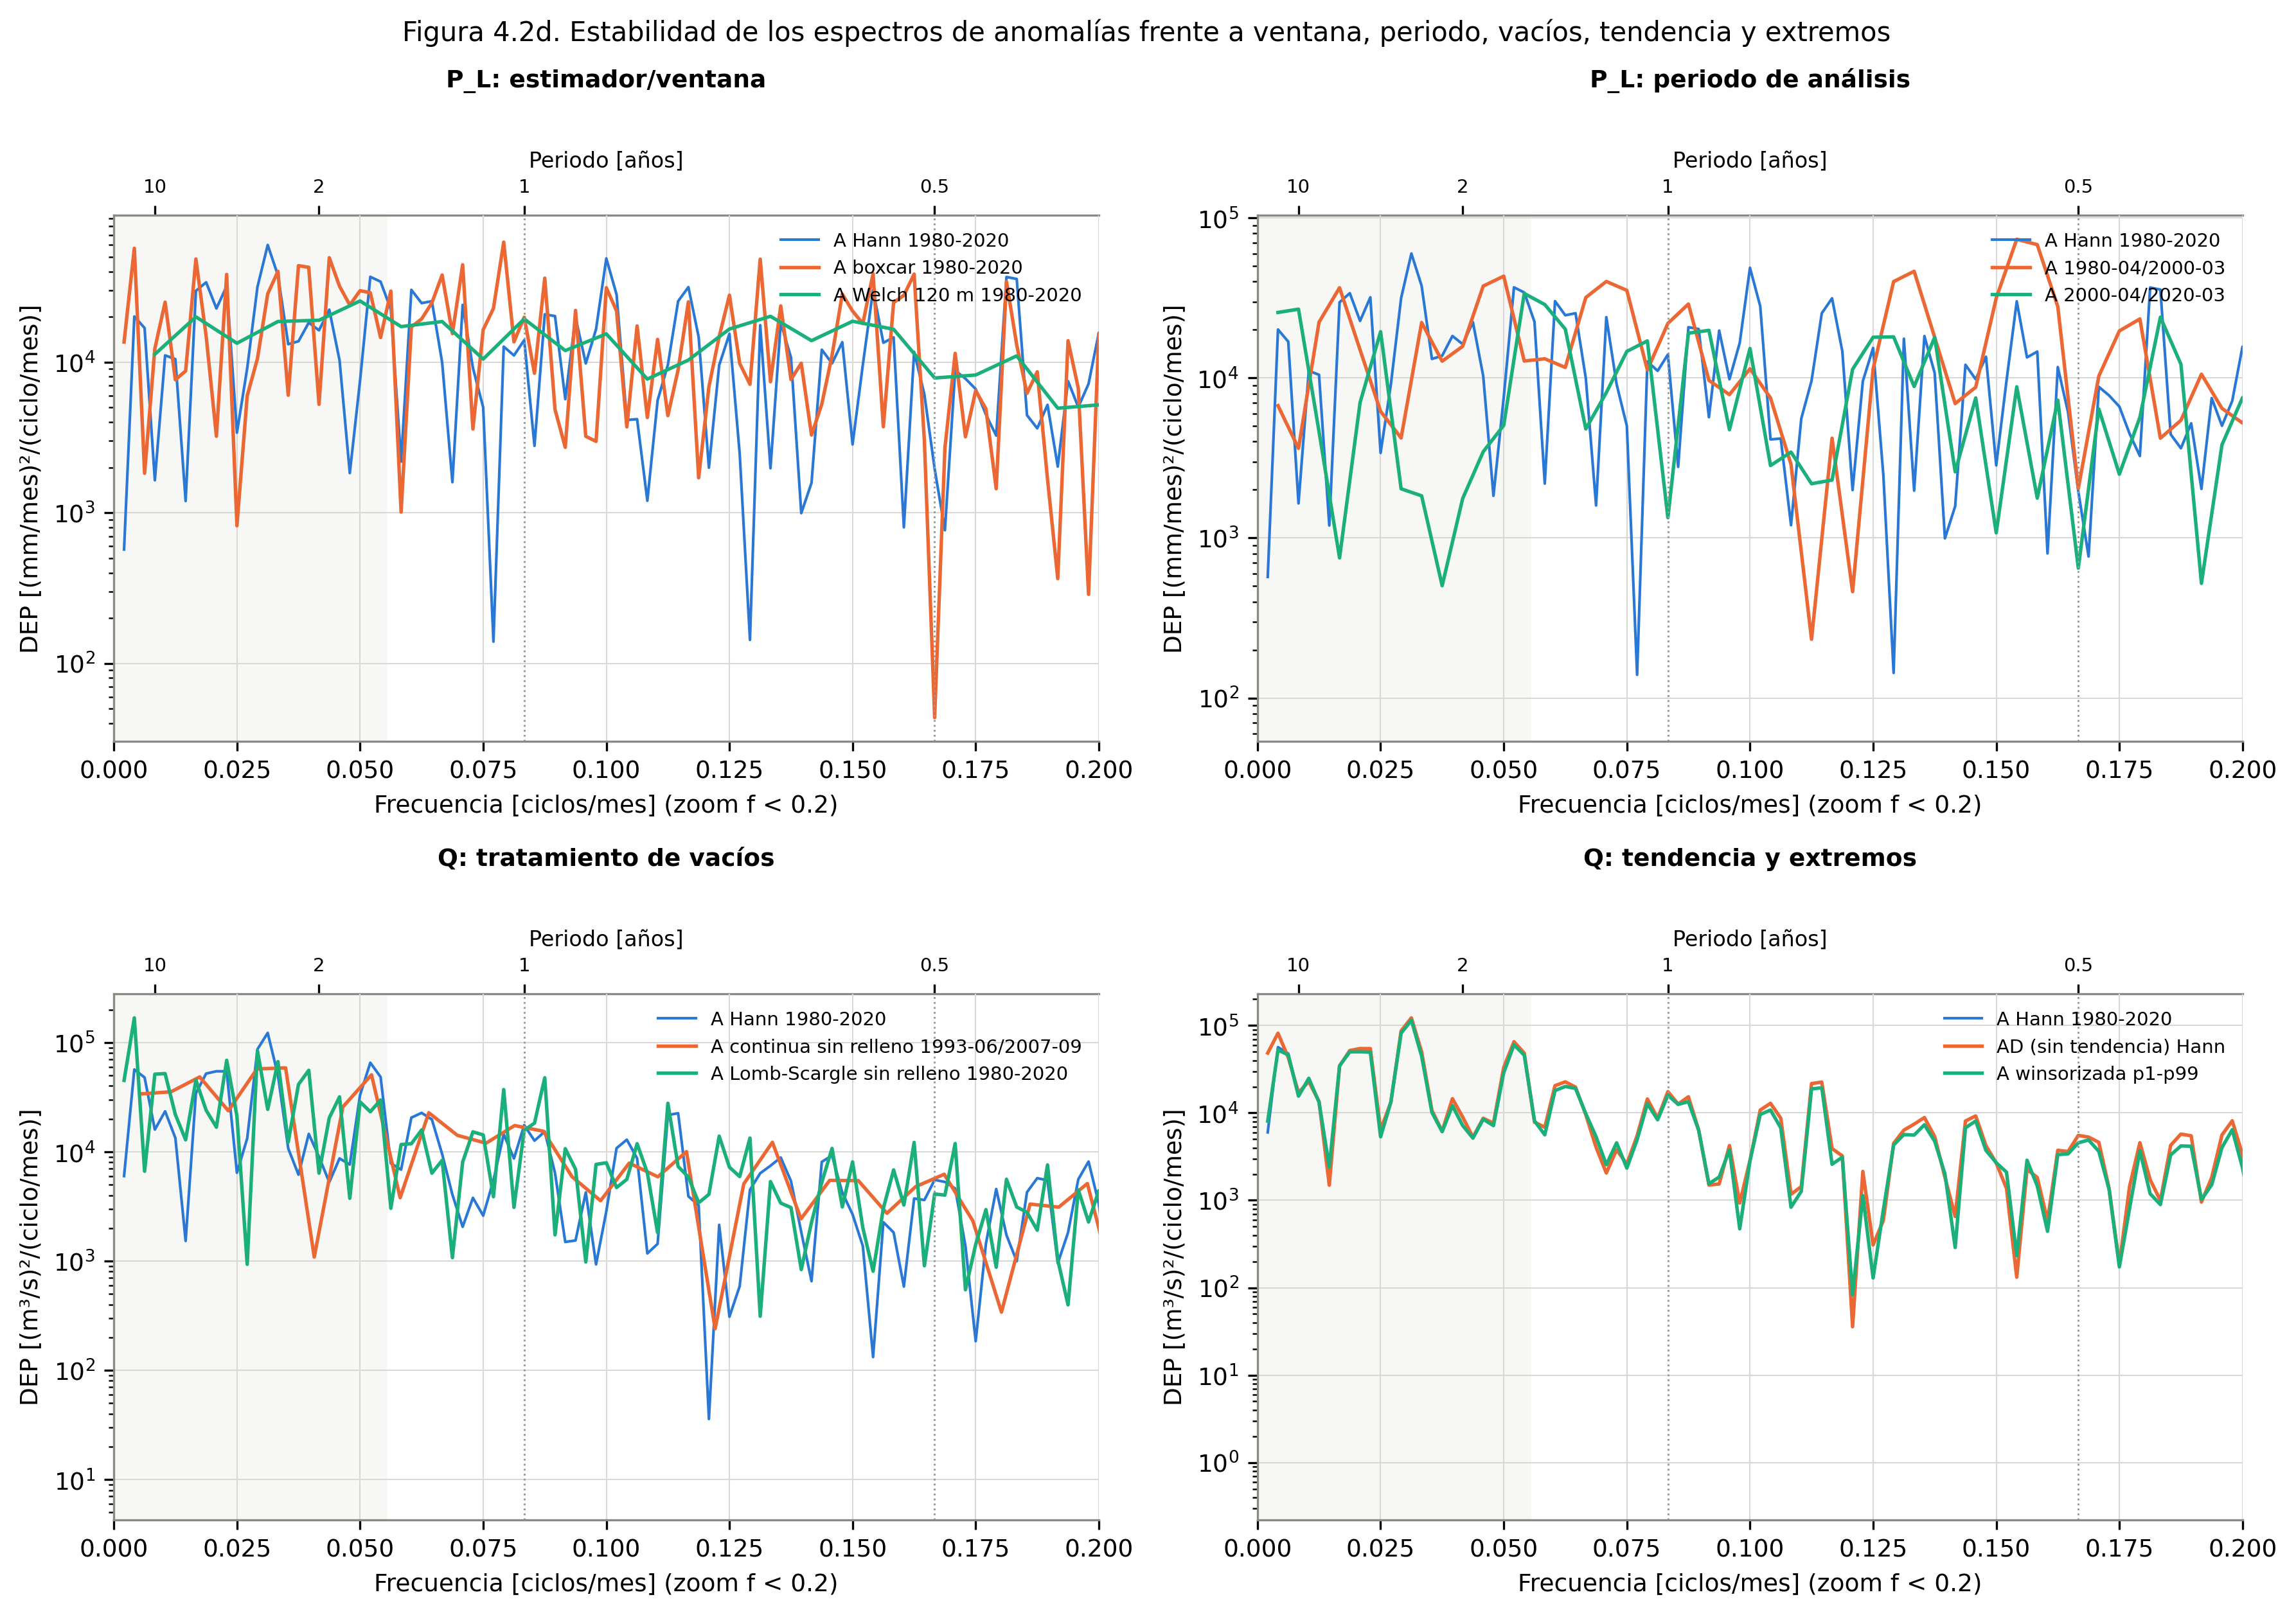
\includegraphics[width=0.92\textwidth]{figura_4_2d_estabilidad.png}
\caption{Estabilidad de los espectros de anomalías frente al estimador, el periodo, el tratamiento de vacíos, la tendencia y los extremos (detalle de $f<0.2$ ciclos/mes).}
\label{fig:estab4}
\end{figure}

\begin{figure}[H]
\centering
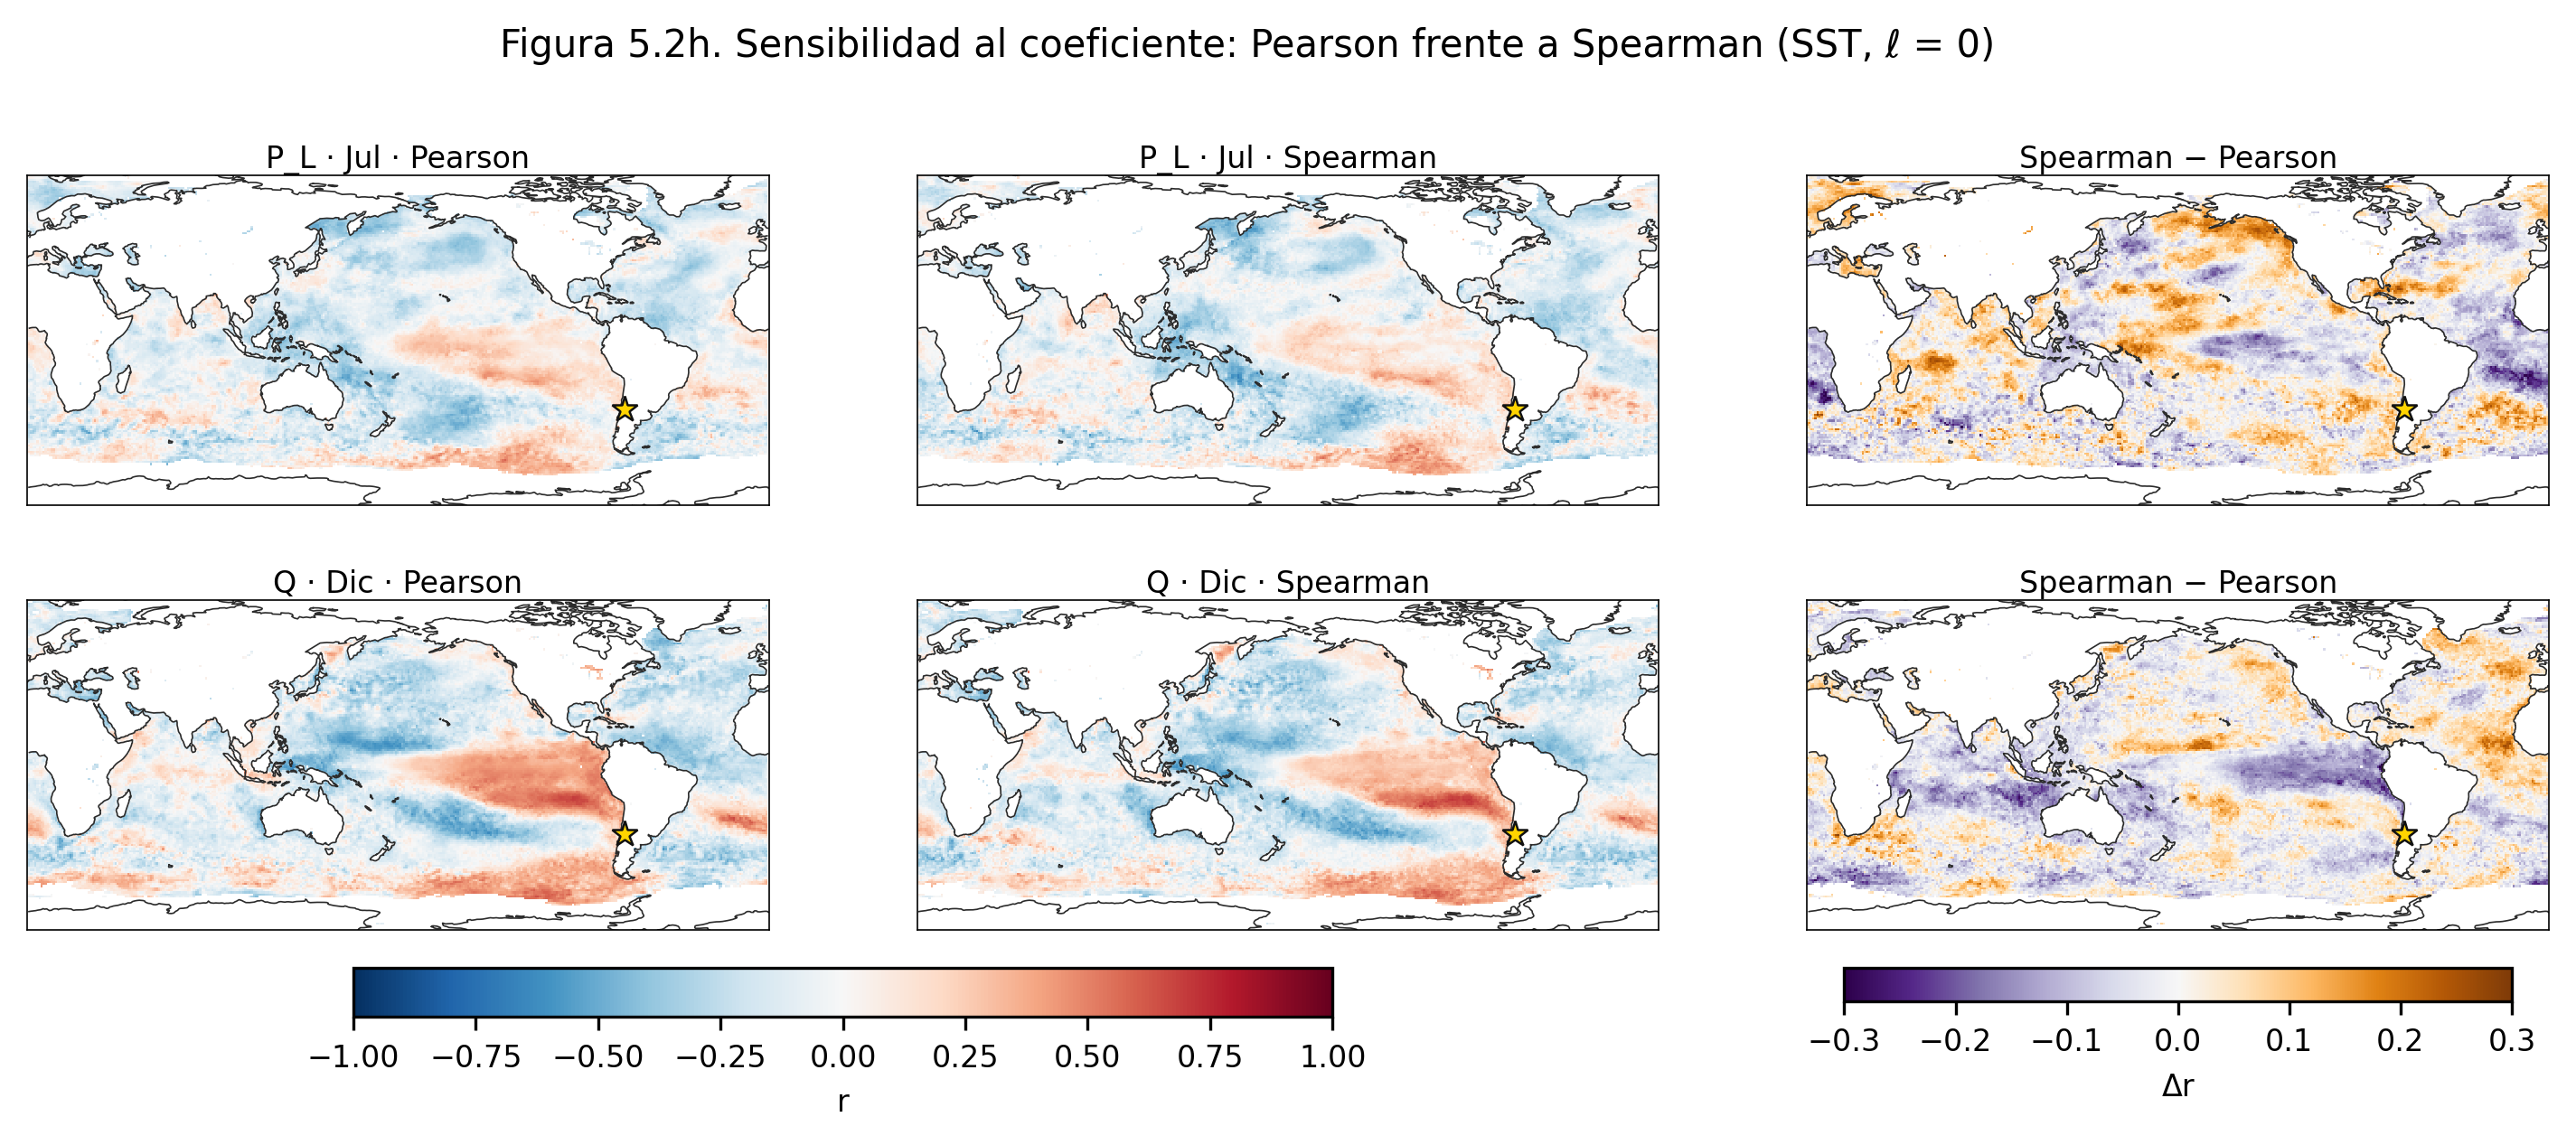
\includegraphics[width=0.85\textwidth]{figura_5_2h_pearson_vs_spearman.png}
\caption{Pearson, Spearman y su diferencia para $\PL$ en julio y $\Qm$ en diciembre frente a la SST.}
\label{fig:spear}
\end{figure}

\begin{figure}[H]
\centering
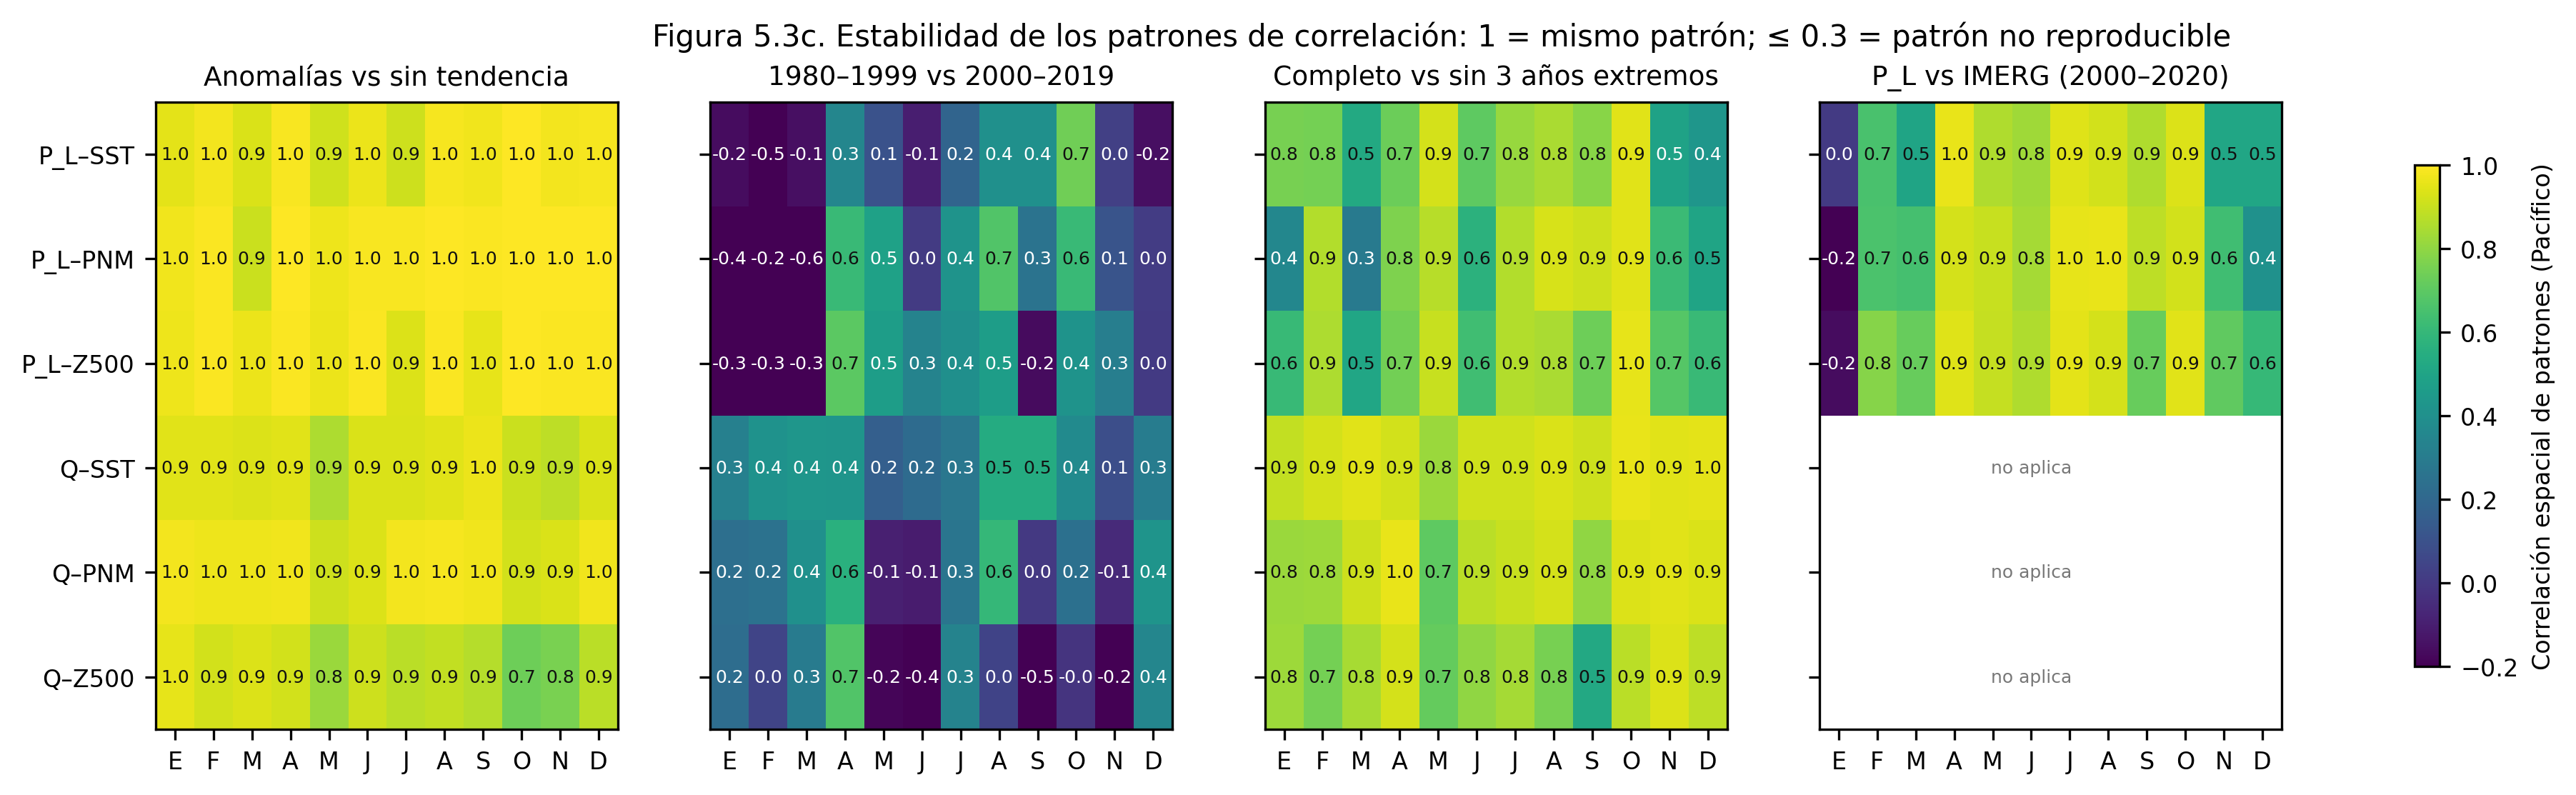
\includegraphics[width=0.95\textwidth]{figura_5_3c_estabilidad.png}
\caption{Correlación espacial de patrones entre configuraciones, por combinación y mes.}
\label{fig:estab5}
\end{figure}

\begin{figure}[H]
\centering
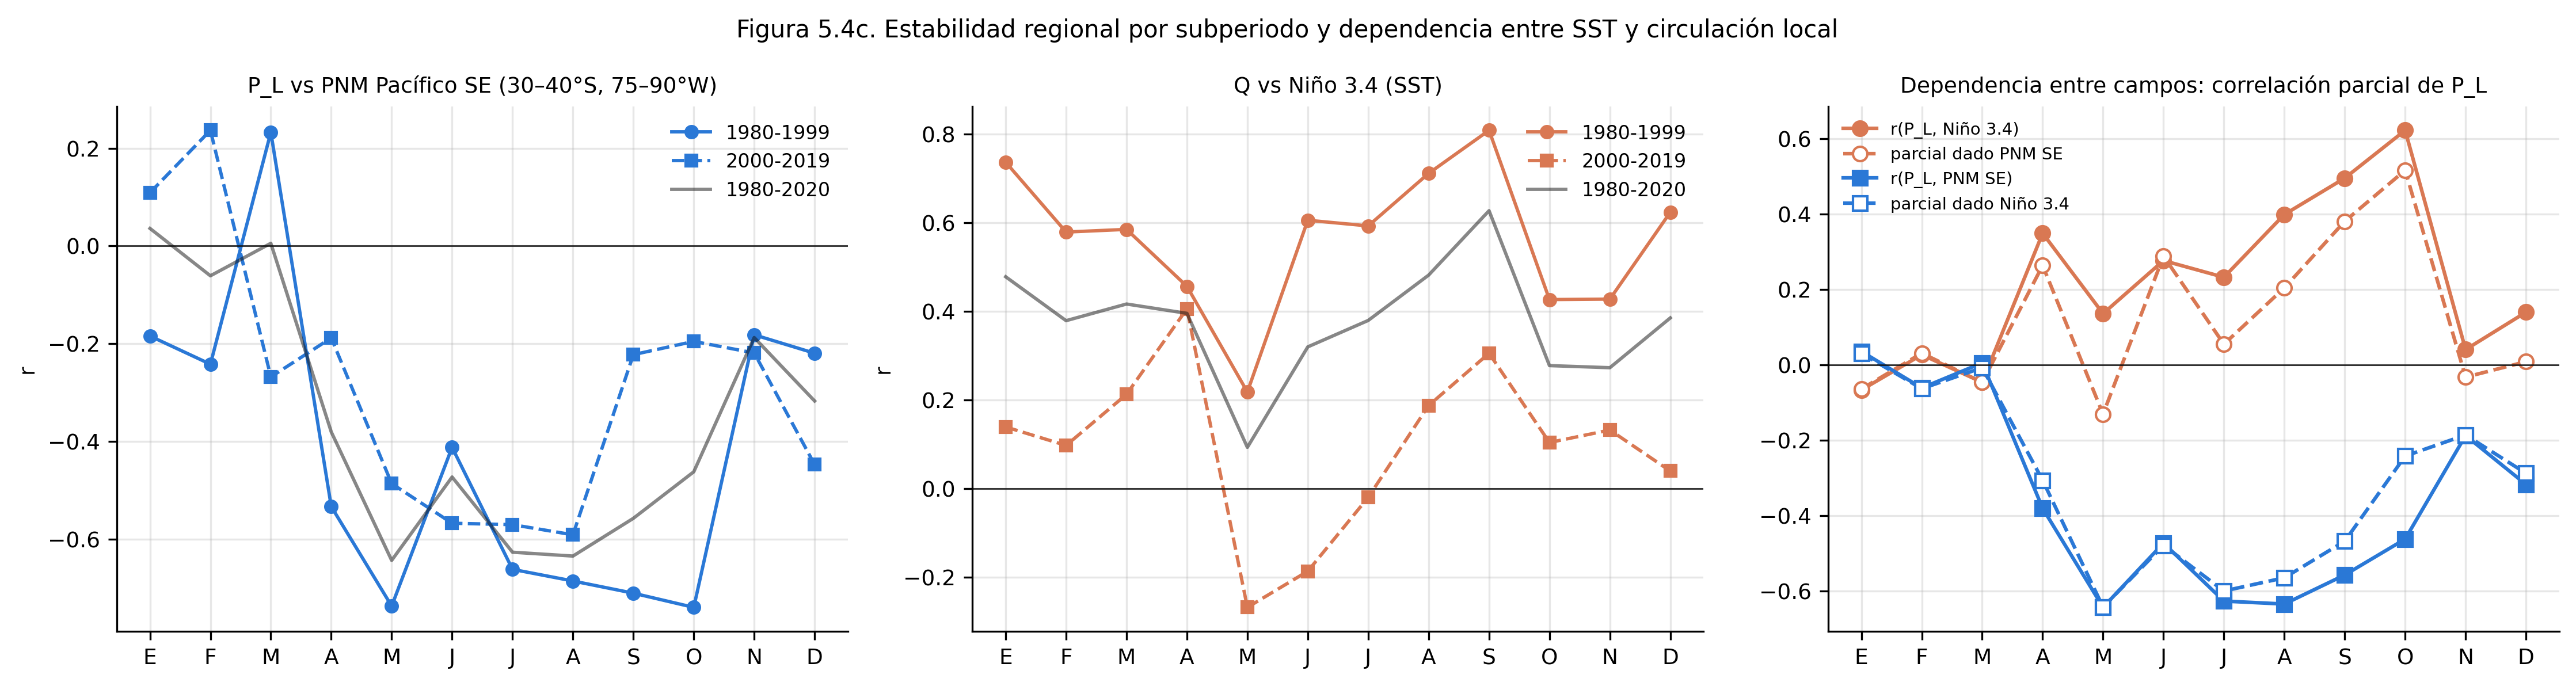
\includegraphics[width=\textwidth]{figura_5_4c_subperiodos_parcial.png}
\caption{Correlación por subperiodo ($\PL$--PNM y $\Qm$--Niño 3.4) y correlación parcial de $\PL$ con Niño 3.4 y con la PNM local.}
\label{fig:sub5}
\end{figure}

\begin{figure}[H]
\centering
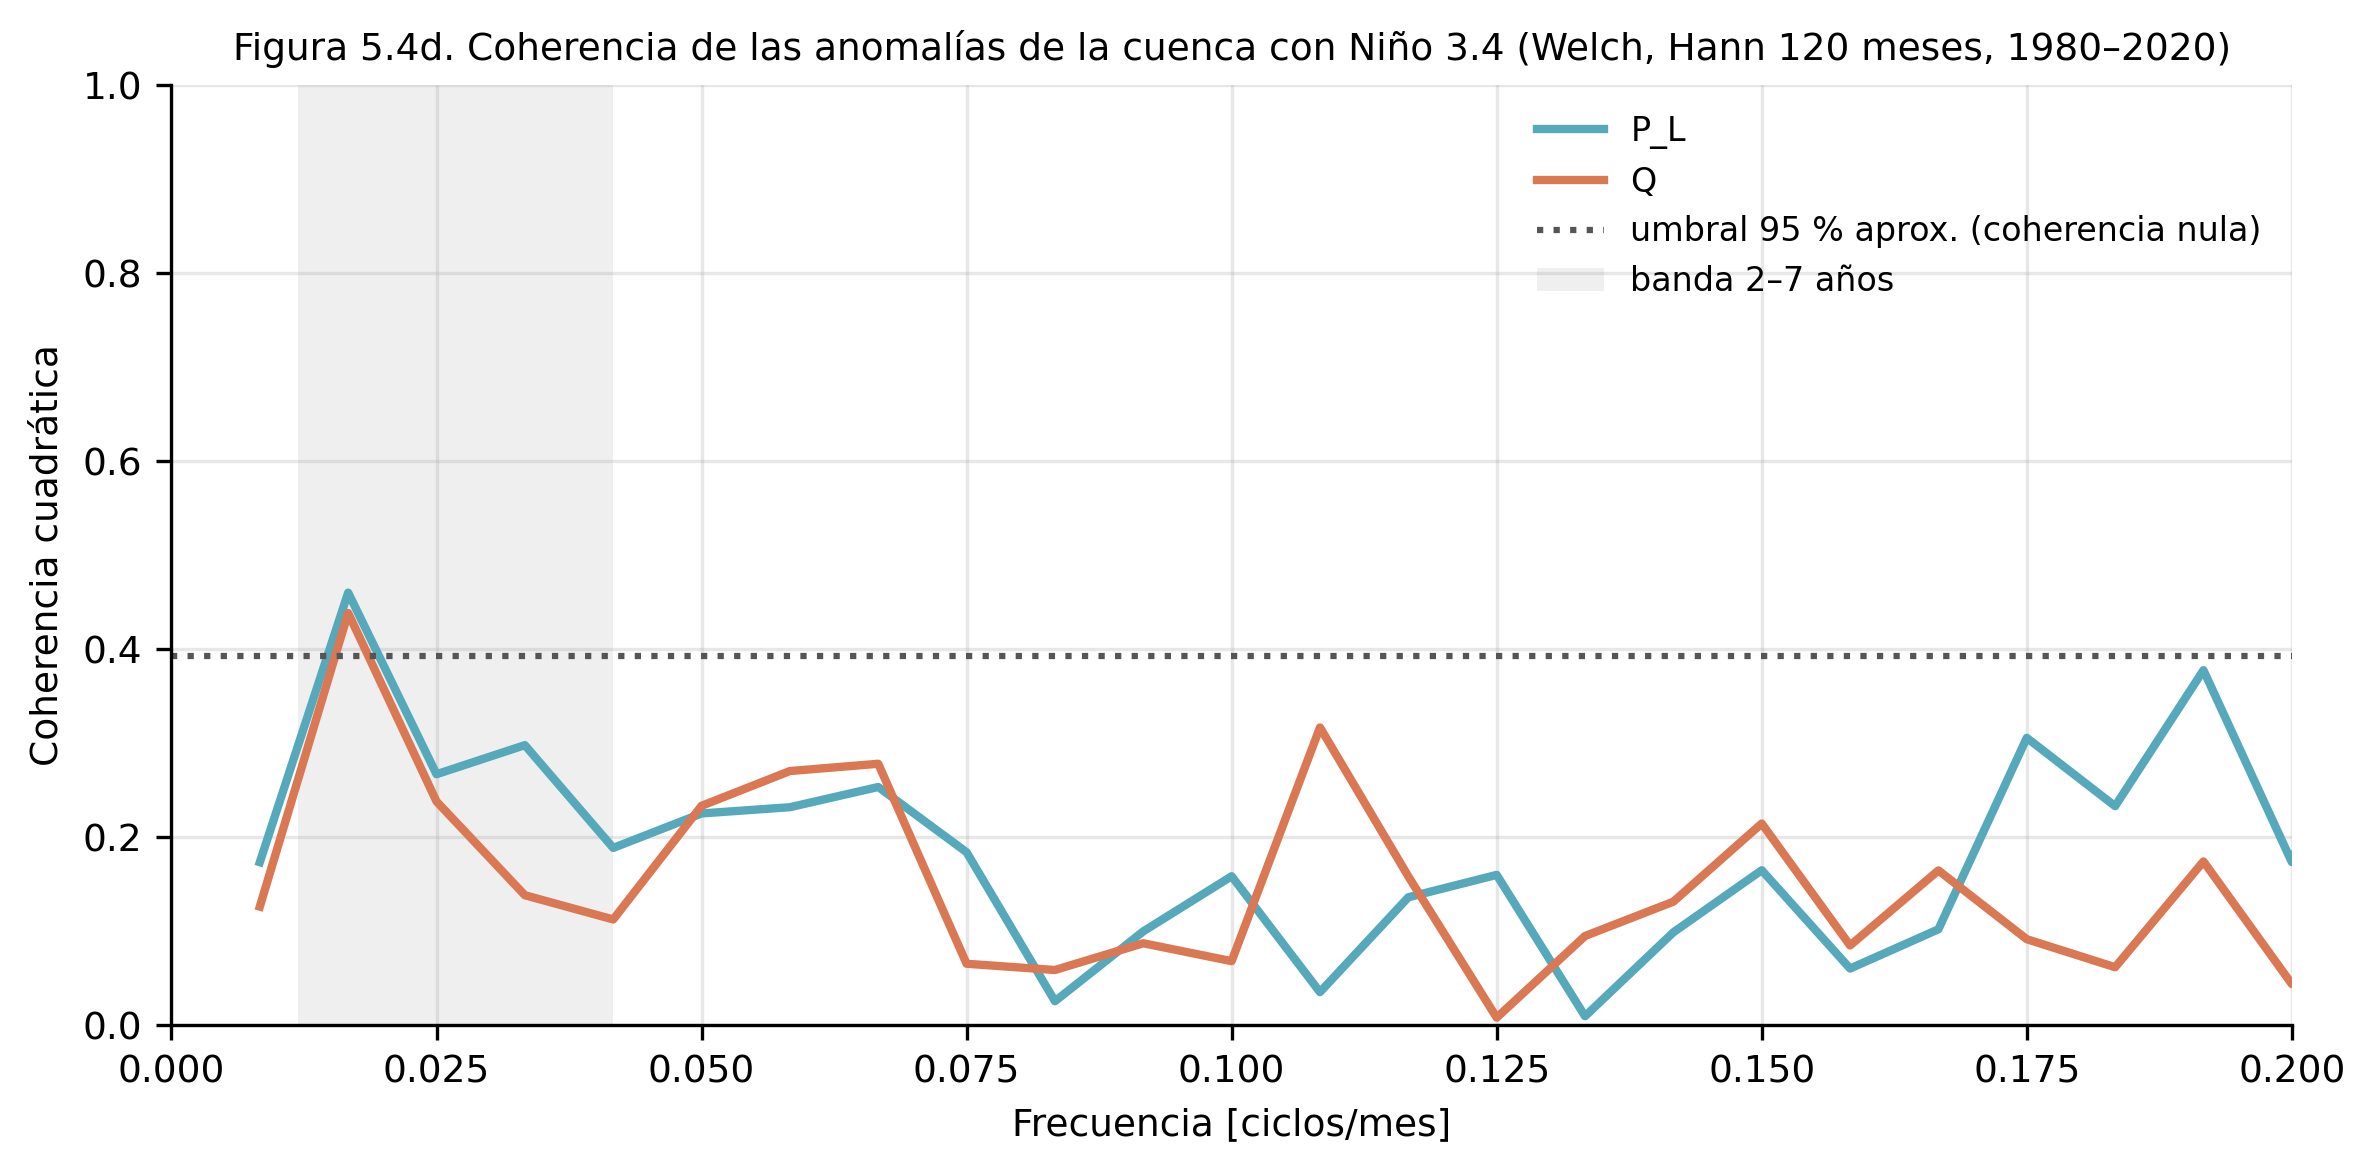
\includegraphics[width=0.62\textwidth]{figura_5_4d_coherencia.png}
\caption{Coherencia cuadrática entre las anomalías de $\PL$ o $\Qm$ y Niño 3.4 (Welch con ventanas Hann de 120 meses, 1980--2020).}
\label{fig:coh5}
\end{figure}
\end{document}
